\documentclass{article}

% if you need to pass options to natbib, use, e.g.:
%     \PassOptionsToPackage{numbers, compress}{natbib}
% before loading neurips_2021

% ready for submission
\usepackage{neurips_2022}

% to compile a preprint version, e.g., for submission to arXiv, add add the
% [preprint] option:
%     \usepackage[preprint]{neurips_2021}

% to compile a camera-ready version, add the [final] option, e.g.:
%     \usepackage[final]{neurips_2021}

% to avoid loading the natbib package, add option nonatbib:
%    \usepackage[nonatbib]{neurips_2021}

\usepackage[utf8]{inputenc} % allow utf-8 input
\usepackage[T1]{fontenc}    % use 8-bit T1 fonts
\usepackage{hyperref}       % hyperlinks
\usepackage{url}            % simple URL typesetting
\usepackage{booktabs}       % professional-quality tables
\usepackage{amsfonts}       % blackboard math symbols
\usepackage{nicefrac}       % compact symbols for 1/2, etc.
\usepackage{microtype}      % microtypography
\usepackage{xcolor}         % colors
\usepackage{enumitem}


%\usepackage{charter}
%\usepackage{calc}

\usepackage{multirow}
% \usepackage[cp1250]{inputenc}
% \usepackage[T1]{fontenc}
% \usepackage{calligra}
\usepackage{layout}

% AMS
\usepackage{amsmath}
\usepackage{amsthm}
\usepackage{amssymb}
\usepackage{amsfonts}
\usepackage{mathtools}
\usepackage{siunitx}

\usepackage{bbm}

\usepackage{url}
\usepackage{color}
\usepackage{graphicx}
\usepackage{algorithmic}
\usepackage{algorithm}
\usepackage{verbatim}

\usepackage{apptools}
\usepackage{thmtools}
% \usepackage{algpseudocode}

% paper specific macros
\newcommand{\g}{{\color{red}g}}
\newcommand{\h}{{\color{blue}h}}

% general macros

\newcommand{\norm}[1]{\left\| #1 \right\|}
\newcommand{\sqnorm}[1]{\left\| #1 \right\|^2}
\newcommand{\lin}[1]{\left\langle #1\right\rangle} % inner product
\newcommand{\inp}[2]{\left\langle#1,#2\right\rangle} % inner product

% caligraphic
\newcommand{\cA}{\mathcal{A}}
\newcommand{\cB}{\mathcal{B}}
\newcommand{\cC}{\mathcal{C}}
\newcommand{\cD}{\mathcal{D}}
\newcommand{\cH}{\mathcal{H}}
\newcommand{\cL}{\mathcal{L}}
\newcommand{\cO}{\mathcal{O}}
\newcommand{\cQ}{\mathcal{Q}}
\newcommand{\cS}{\mathcal{S}}
\newcommand{\cW}{\mathcal{W}}
\newcommand{\cY}{\mathcal{Y}}
\newcommand{\cZ}{\mathcal{Z}}

% bold matrices
\newcommand{\mM}{\mathbf{M}}
\newcommand{\mN}{\mathbf{N}}
\newcommand{\mI}{\mathbf{I}}
\newcommand{\mJ}{\mathbf{J}}
\newcommand{\mL}{\mathbf{L}}
\newcommand{\mD}{\mathbf{D}}
\newcommand{\mO}{\mathbf{O}}


% strange stuff
\newcommand{\hotidea}{{\color{red}\bf HOT IDEA: }}
\newcommand{\done}{{\color{blue}\bf DONE: }}
\newcommand{\del}[1]{}
\let\la=\langle
\let\ra=\rangle

% basic macros
\newcommand{\R}{\mathbb{R}} % reals
\newcommand{\U}{\mathbb{U}} % reals
\newcommand{\PermComp}{\U\mathbb{P}} % reals

\newcommand{\st}{\;:\;} % such that
%\newcommand{\eqdef}{\stackrel{\text{def}}{=}}
\newcommand{\eqdef}{:=} %\vcentcolon

\newcommand{\Prob}{\mathbf{Prob}} % probability
\newcommand{\ProbCond}[2]{\Prob\left(\left.#1\right\vert#2\right)}

\newcommand{\nnz}[1]{{\color{red}\|#1\|_0}}

% sets
\DeclareMathOperator{\card}{card}         % cardinality of a set
\DeclareMathOperator{\diam}{diam}        % diameter of a set
\DeclareMathOperator{\vol}{vol}               % volume of a set

% statistics
\newcommand{\Exp}[1]{{\rm E}\left[#1\right]}
\newcommand{\ExpCond}[2]{{\rm E}\left[\left.#1\right\vert#2\right]}
\newcommand{\ExpSub}[2]{{\rm E}_{#1}\left[#2\right]}
\DeclareMathOperator{\Cov}{Cov}         % covariance
\DeclareMathOperator{\Var}{Var}         % variance
\DeclareMathOperator{\Corr}{Corr}       % correlation

% functions and operators
\DeclareMathOperator{\signum}{sign}     % signum/sign of a scalar
\DeclareMathOperator{\dom}{dom}         % domain
\DeclareMathOperator{\epi}{epi}         % epigraph
\DeclareMathOperator{\Ker}{null}        % nullspace/kernel
\DeclareMathOperator{\nullspace}{null}  % nullpsace
\DeclareMathOperator{\range}{range}     % range
\DeclareMathOperator{\Image}{Im}        % image

% topology
\DeclareMathOperator{\interior}{int}    % interior
\DeclareMathOperator{\ri}{rint}         % relative interior
\DeclareMathOperator{\rint}{rint}       % relative interior
\DeclareMathOperator{\bdry}{bdry}       % boundary
\DeclareMathOperator{\cl}{cl}           % closure

% vectors, matrices
\DeclareMathOperator{\linspan}{span}
\DeclareMathOperator{\linspace}{linspace}
\DeclareMathOperator{\cone}{cone}

\DeclareMathOperator{\tr}{tr}           % trace
\DeclareMathOperator{\rank}{rank}       % rank
\DeclareMathOperator{\conv}{conv}       % convex hull
\DeclareMathOperator{\Diag}{Diag}       % Diag(v) = diagonal matrix with v_i on the diagonal
\DeclareMathOperator{\diag}{diag}       % diag(D) = the diagonal vector of matrix D
\DeclareMathOperator{\Arg}{Arg}         % Argument

%\renewcommand{\qedsymbol}{\ding{114}}




%%%%%%%%

% TODO: Fix here fonts
\newcommand{\Sample}{\mathcal{S}}
%\newcommand{\E}{\mathbb{E}}
%\newcommand{\norm}[1]{\left\lVert#1\right\rVert_2}
\newcommand{\B}{\mathbb{B}}


\usepackage{tcolorbox}
\usepackage{pifont}
\definecolor{mydarkgreen}{RGB}{39,130,67}
\definecolor{mydarkred}{RGB}{192,47,25}
\newcommand{\green}{\color{mydarkgreen}}
\newcommand{\red}{\color{mydarkred}}
\newcommand{\cmark}{\green\ding{51}}%
\newcommand{\xmark}{\red\ding{55}}%

\newcommand{\algname}[1]{{\green\small \sf #1}}
\newcommand{\algnamesmall}[1]{{\green\scriptsize \sf #1}}

\newcommand{\tablescriptsize}[1]{{\scriptsize #1}}
\newcommand{\tablesmall}[1]{{\small #1}}



%%%%%%%%

\newtheorem{assumption}{Assumption}
\newtheorem{lemma}{Lemma}
\newtheorem{algorithms}{Algorithm}
\newtheorem{theorem}{Theorem}
\newtheorem{proposition}{Proposition}
\newtheorem{example}{Example}
\newtheorem{corollary}{Corollary}

\theoremstyle{plain}

\newtheorem{prop}[theorem]{Proposition}
\newtheorem{cor}[theorem]{Corollary}
\newtheorem{lem}[theorem]{Lemma}
\newtheorem{claim}[theorem]{Claim}
\newtheorem{remark}[theorem]{Remark}

\theoremstyle{definition}

\newtheorem{exercise}[theorem]{Exercise}

\newtheorem{rem}[theorem]{Remark}
\newtheorem{que}[theorem]{Question}
\newtheorem{definition}[theorem]{Definition}

% Hack that enables labeling of lines in algorithms
\newcommand{\alglinelabel}{%
  \addtocounter{ALC@line}{-1}% Reduce line counter by 1
  \refstepcounter{ALC@line}% Increment line counter with reference capability
  \label% Regular \label
}
\usepackage[textsize=tiny]{todonotes}
\usepackage{footnote}
\usepackage{mathtools}
\usepackage[flushleft]{threeparttable}

\newcommand{\alexander}[1]{\todo[inline]{\textbf{Alexander: }#1}}

\newcommand{\algorithmname}{DASHA-PP}

\newcommand*{\probavailable}{\ensuremath{p_{\textnormal{a}}}}
\newcommand*{\probpairaa}{\ensuremath{p_{\textnormal{aa}}}}
\newcommand*{\probpairan}{\ensuremath{p_{\textnormal{an}}}}
\newcommand*{\probpairnn}{\ensuremath{p_{\textnormal{nn}}}}

\newcommand*{\probpage}{\ensuremath{p_{\text{page}}}}
\newcommand*{\probmega}{\ensuremath{p_{\text{mega}}}}

\allowdisplaybreaks
\makeatletter
\newcommand{\vast}{\bBigg@{4}}
\newcommand{\Vast}{\bBigg@{5}}
\makeatother

\newcommand{\improvement}[1]{{\color{orange}#1}}
\newcommand{\degeneration}[1]{{\color{red}#1}}

\title{A Computation and Communication Efficient Method for Distributed Nonconvex Problems in the Partial Participation Setting}

% The \author macro works with any number of authors. There are two commands
% used to separate the names and addresses of multiple authors: \And and \AND.
%
% Using \And between authors leaves it to LaTeX to determine where to break the
% lines. Using \AND forces a line break at that point. So, if LaTeX puts 3 of 4
% authors names on the first line, and the last on the second line, try using
% \AND instead of \And before the third author name.

\author{%
  Alexander Tyurin\\
  KAUST\\
  Saudi Arabia\\
  \texttt{alexandertiurin@gmail.com} \\
  \And
  Peter Richt\'{a}rik \\
  KAUST\\
  Saudi Arabia\\
  \texttt{richtarik@gmail.com} \\
}

\begin{document}

\maketitle

\begin{abstract}
  We present a new method that includes three key components of distributed optimization and federated learning: the variance reduction of stochastic gradients, compressed communication, and partial participation. We prove that the new methods have the optimal oracle complexity and the state-of-the-art communication complexity in the partial participation setting. Moreover, we observe that "1 + 1 + 1 is not 3": by mixing the variance reduction of stochastic gradients with compressed communication and partial participation, we catch side effects in theory. We explain their nature and possible workarounds.
\end{abstract}

\section{Introduction}
Federated and distributed learning have become very popular in recent years \citep{konevcny2016federated, mcmahan2017communication}. 
The current optimization tasks require much computational resources and machines. Such requirements emerge in machine learning, where massive datasets and computations are distributed between cluster nodes \citep{lin2017deep, ramesh2021zero}. In federated learning, nodes, represented by mobile phones, laptops, and desktops, do not send their data to a server due to privacy and their huge number \citep{ramaswamy2019federated}, and the server remotely orchestrates the nodes and communicates with them to solve an optimization problem.

As in classical optimization tasks, one of the main current challenges is to find \textbf{computationally efficient} optimization algorithms. However, the nature of distributed problems induces many other \citep{kairouz2021advances}, including i) \textbf{partial participation} of nodes in algorithm steps: due to stragglers \citep{li2020federated} or communication delays \citep{vogels2021relaysum}, ii) \textbf{communication bottleneck}: even if a node participates, it can be costly to transmit information to a server or other nodes \citep{alistarh2017qsgd, ramesh2021zero,kairouz2021advances, sapio2019scaling, narayanan2019pipedream}. It is necessary to develop a method that considers these problems.

% \begin{enumerate}
%   \item Partial Participation (No Synchronization)
%   \item Variance Reduction
%   \item Compression
% \end{enumerate}

\section{Optimization Problem}
Let us consider the nonconvex distributed optimization problem
\begin{align}
    \label{eq:main_problem} 
    \min \limits_{x \in \R^d}\left\{f(x) \eqdef \frac{1}{n}\sum \limits_{i=1}^n f_i(x)\right\},
\end{align}
where $f_i\,:\,\R^d \rightarrow \R$ is a smooth nonconvex function for all $i \in [n] \eqdef \{1, \dots, n\}.$ The full information about function $f_i$ is stored on $i$\textsuperscript{th} node. The communication between nodes is maintained in the parameters server fashion \citep{kairouz2021advances}: we have a server that receives compressed information from nodes, updates a state, and broadcasts an updated model.\footnote{Note that this strategy can be used in peer-to-peer communication, assuming that the server is an abstraction and all its algorithmic steps are performed on each node.} Since we work in the nonconvex world, our goal is to find an $\varepsilon$-solution ($\varepsilon$-stationary point) of \eqref{eq:main_problem}: a (possibly random) point $\widehat{x}\in \R^d$, such that ${\rm E}\big[\norm{\nabla f(\widehat{x})}^2\big] \leq \varepsilon.$

We consider three settings:
\begin{enumerate}[leftmargin=0.75cm]
\item \textbf{Gradient Setting.}
The $i$\textsuperscript{th} node has only access to the gradient $\nabla f_i \,:\,\R^d \rightarrow \R^d$ of function $f_i$. Moreover, the following assumptions for the functions $f_i$ hold.
\begin{assumption}
    \label{ass:lower_bound}
    There exists $f^* \in \R$ such that $f(x) \geq f^*$ for all $x \in \R$.
\end{assumption}
\begin{assumption}
    \label{ass:lipschitz_constant}
    The function $f$ is $L$--smooth for all $i \in [n]$, i.e., $\norm{\nabla f(x) - \nabla f(y)} \leq L \norm{x - y}$ for all $x, y \in \R^d.$
\end{assumption}
\begin{assumption} \leavevmode
    \label{ass:nodes_lipschitz_constant}
    The functions $f_i$ are $L_i$--smooth. Let us define $\widehat{L}^2 \eqdef \frac{1}{n} \sum_{i=1}^{n} L_i^2.$\footnote{Note that $L \leq \widehat{L},$ $\widehat{L} \leq L_{\max},$ and $\widehat{L} \leq L_{\sigma}.$}
\end{assumption}

\item \textbf{Finite-Sum Setting.}
The functions $\{f_i\}_{i=1}^n$ have the finite-sum form
\begin{align}
    \label{eq:task_minibatch} f_i(x) = \frac{1}{n}\sum \limits_{j=1}^m f_{ij}(x), \qquad \forall i \in [n],
\end{align}
where $f_{ij} :\R^d  \rightarrow \R$ is a smooth nonconvex  function for all $j \in [m].$
We assume that Assumptions~\ref{ass:lower_bound}, \ref{ass:lipschitz_constant} and \ref{ass:nodes_lipschitz_constant} hold and the following assumption.
\begin{assumption}
  \label{ass:max_lipschitz_constant}
  The function $f_{ij}$ is $L_{ij}$-smooth for all $i \in [n], j \in [m].$ Let $L_{\max} \eqdef \max_{i \in [n], j \in [m]} L_{ij}.$
\end{assumption}
\item \textbf{Stochastic Setting.}
The function $f_i$ is an expectation of a stochastic function, 
\begin{align}
    \label{eq:task_staochastic}
    f_i(x) = \ExpSub{\xi}{f_i(x;\xi)}, \qquad \forall i \in [n],
\end{align}
where $f_i :\R^d \times \Omega_{\xi} \rightarrow \R.$ For a fixed $x \in \R,$ $f_i(x;\xi)$ is a random variable over some distribution $\mathcal{D}_i$,
and, for a fixed $\xi \in \Omega_{\xi},$ $f_i(x;\xi)$ is a smooth nonconvex function.
The $i$\textsuperscript{th} node has only access to a stochastic gradients $\nabla f_i(\cdot; \xi_{ij})$ 
of the function $f_i$ through the distribution $\mathcal{D}_i,$ where $\xi_{ij}$ is a sample from $\mathcal{D}_i.$
We assume that Assumptions~\ref{ass:lower_bound}, \ref{ass:lipschitz_constant} and \ref{ass:nodes_lipschitz_constant} hold and the following assumptions.
\begin{assumption}
  \label{ass:stochastic_unbiased_and_variance_bounded}
  For all $i \in [n]$ and for all $x \in \R^d,$ the stochastic gradient $\nabla f_i(x;\xi)$ is unbiased and has bounded variance, i.e., $\ExpSub{\xi}{\nabla f_i(x;\xi)} = \nabla f_i(x),$ and $\ExpSub{\xi}{\norm{\nabla f_i(x;\xi) - \nabla f_i(x)}^2} \leq \sigma^2,$ where $\sigma^2 \geq 0.$
\end{assumption}
\begin{assumption}
  \label{ass:mean_square_smoothness}
  For all $i \in [n]$ and for all $x, y \in \R,$ the stochastic gradient $\nabla f_i(x;\xi)$ satisfies the mean-squared smoothness property, i.e., $\ExpSub{\xi}{\norm{\nabla f_i(x;\xi) - \nabla f_i(y;\xi)}^2} \leq L_{\sigma}^2 \norm{x - y}^2.$
\end{assumption}
\end{enumerate}
We compare algorithms using \textit{the oracle complexity}, i.e., the number of (stochastic) gradients that each node has to calculate to get $\varepsilon$-solution, and \textit{the communication complexity}, i.e., the number of bits that each node has to send to the server to get $\varepsilon$-solution.

\subsection{Unbiased Compressors}
We use the concept of unbiased compressors to alleviate the communication bottleneck. The unbiased compressors quantize and/or sparsify vectors that the nodes send to the server.
\begin{definition}
    \label{def:unbiased_compression}
    A stochastic mapping $\cC\,:\,\R^d \rightarrow \R^d$ is an \textit{unbiased compressor} if
    there exists $\omega \in \R$ such that
    \begin{align}
        \label{eq:compressor}
        \hspace{-0.2cm}\Exp{\cC(x)} = x, \qquad \Exp{\norm{\cC(x) - x}^2} \leq \omega \norm{x}^2, \qquad \forall x \in \R^d.
    \end{align}
\end{definition}
We denote a set of stochastic mappings that satisfy Definition~\ref{def:unbiased_compression} as $\mathbb{U}(\omega).$
In our methods, the nodes make use of unbiased compressors $\{\cC_i\}_{i=1}^n.$ 
The community developed a large number of unbiassed compressors, including Rand$K$ (see Definition~\ref{def:rand_k}) \citep{beznosikov2020biased, stich2018sparsified}, Adaptive sparsification \citep{wangni2018gradient} and Natural compression and dithering \citep{horvath2019natural}. We are aware of correlated compressors by \cite{szlendak2021permutation} and quantizers by \cite{suresh2022correlated} that help in the homogeneous regimes, but in this work, we are mainly concentrated on generic heterogeneous regimes, though, for simplicity, assume the independence of the compressors.
\begin{assumption}
\label{ass:compressors}
 $\cC_i \in \mathbb{U}(\omega)$ for all $i\in [n]$, and the compressors are  \textit{independent}.
\end{assumption}

\subsection{Nodes Partial Participation Assumptions}
\label{sec:partial_participation}

\newcommand\Item[1][]{%
  \ifx\relax#1\relax  \item \else \item[#1] \fi
  \abovedisplayskip=0pt\abovedisplayshortskip=0pt~\vspace*{-\baselineskip}}

We now try to formalize the notion of partial participation. Let us assume that we have $n$ events $\{i^{\textnormal{th}} \textnormal{ node is \textit{participating}}\}$ with the following properties.
\begin{assumption}
  \label{ass:partial_participation}
  The partial participation of nodes has the following distribution: exists constants $\probavailable \in (0, 1]$ and $\probpairaa \in [0, 1],$ such that
  \begin{enumerate}
    \Item \begin{align*}\Prob\left(i^{\textnormal{th}} \textnormal{ node is \textit{participating}}\right) = \probavailable, \quad \forall i \in [n],\end{align*}
    \Item \begin{align*}\Prob\left(i^{\textnormal{th}} \textnormal{ node is \textit{participating}}, j^{\textnormal{th}} \textnormal{ node is \textit{participating}}\right) = \probpairaa, \quad \forall i \neq j \in [n],\end{align*}
    \Item \begin{align} \label{eq:partial_participation_constraint}
      \probpairaa \leq \probavailable^2,
    \end{align}
  \end{enumerate}
  and these events from different communication rounds are independent.
\end{assumption}

We are not fighting for the full generality and believe that more complex sampling strategies can be considered in the analysis. For simplicity, we settle upon Assumption~\ref{ass:partial_participation}. Standard partial participation strategies, including $s$--nice sampling, where the server chooses uniformly $s$ nodes without replacement ($\probavailable = \nicefrac{s}{n}$ and $\probpairaa~=~\nicefrac{s(s-1)}{n(n-1)}$),
and independent participation, where each node independently participates with probability $\probavailable$ (due to independence, we have $\probpairaa = \probavailable^2$), satisfy Assumption~\ref{ass:partial_participation}. In the literature, $s$--nice sampling is one of the most popular strategies \citep{zhao2021faster, fatkhullin2021ef21, reddi2020adaptive, konevcny2016federated}. 

\section{Motivation and Related Work}
The main goal of our paper is to develop a method for the nonconvex distributed optimization that will include three key features: variance reduction of stochastic gradients, compressed communication, and partial participation.

\textbf{1. Variance reduction of stochastic gradients}\\
It is important to consider finite-sum \eqref{eq:task_minibatch} and stochastic \eqref{eq:task_staochastic} settings because, in machine learning tasks, either the number of local functions $m$ is huge or the functions $f_i$ is an expectation of a stochastic function due to the batch normalization \citep{ioffe2015batch} or random augmentation \citep{goodfellow2016deep}, and it is infeasible to calculate the full gradients analytically. Let us recall the results from the nondistributed optimization. In the gradient setting, the optimal oracle complexity is $\cO\left(\nicefrac{1}{\varepsilon}\right)$, achieved by the vanilla gradient descent (\algname{GD}) \citep{carmon2020lower, nesterov2018lectures}. In the finite-sum setting and stochastic settings, the optimal oracle complexities are $\cO\left(m + \frac{\sqrt{m}}{\varepsilon}\right)$ and $\cO\left(\frac{\sigma^2}{\varepsilon} + \frac{\sigma}{\varepsilon^{\nicefrac{3}{2}}}\right)$ \citep{SPIDER, PAGE, arjevani2019lower}, accordingly, achieved by methods from \citep{SPIDER,SARAH,PAGE}. 
% In our distributed method, we want to maintain the optimal oracle complexities.

\textbf{2. Compressed communication} \\
In distributed optimization \citep{ramesh2021zero, xu2021grace}, lossy communication compression can be a powerful tool to increase the communication speed between the nodes and the server. Different types of compressors are considered in the literature, including unbiased compressors \citep{alistarh2017qsgd,beznosikov2020biased,szlendak2021permutation}, contractive (biased) compressors \citep{EF21}, 3PC compressors \citep{richtarik20223pc}. We will focus on unbiased compressors because methods \citep{tyurin2022dasha, szlendak2021permutation, MARINA} that employ unbiased compressors provide the current theoretical state-of-the-art (SOTA) communication complexities.

Many methods analyzed optimization methods with the unbiased compressors \citep{alistarh2017qsgd, DIANA, horvath2019stochastic, gorbunov2021marina, tyurin2022dasha}. In the gradient setting, the methods by \cite{MARINA} and \cite{tyurin2022dasha} establish the current SOTA communication complexity, each method needs $\frac{1 + \nicefrac{\omega}{n}}{\varepsilon}$ communication rounds to get an $\varepsilon$--solution. In the finite-sum and stochastic settings, the current SOTA communication complexity is attained by methods from \citep{tyurin2022dasha}, while maintaining the optimal oracle complexities $\cO\left(m + \frac{\sqrt{m}}{\varepsilon \sqrt{n}}\right)$ and $\cO\left(\frac{\sigma^2}{\varepsilon n} + \frac{\sigma}{\varepsilon^{\nicefrac{3}{2}} n}\right)$ per node.

\textbf{3. Partial participation} \\
From the beginning of federated learning era, the partial participation has been considered to be the essential feature of distributed optimization methods \citep{mcmahan2017communication, konevcny2016federated, kairouz2021advances}. 
However, previously proposed methods have limitations: i) methods from \citep{gorbunov2021marina, zhao2021fedpage} still require synchronization of all nodes with a small probability, ii) in the stochastic settings, proposed methods with the partial participation mechanism \citep{tyurin2022dasha, zhao2021faster} provide results without variance reduction techniques from \citep{SPIDER, PAGE, cutkosky2019momentum} and, therefore, get suboptimal oracle complexities, iii) in the finite-sum setting, the work by \cite{li2021zerosarah} focuses on the homogeneous regime only (the functions $f_i$ are equal).

\section{Contributions}
We propose a \textit{new family of methods} \algname{\algorithmname} for the nonconvex distributed optimization. As far as we know, this is the first method that includes three key ingredients of federated learning methods: \textit{variance reduction of stochastic gradients, compressed communication, and partial participation}. We prove convergence rates and show that these methods have \textit{the optimal oracle complexity and the state-of-the-art communication complexity in the partial participation setting.} Moreover, in our work, we observe a nontrivial side-effect from mixing the variance reduction of stochastic gradients and partial participation. It is a general problem not related to our methods or analysis that we discuss in Section~\ref{sec:partial_participation_sampling}.

\section{Algorithm Description}

We now present \algname{\algorithmname} (see Algorithm~\ref{alg:main_algorithm}), a family of methods to solve the optimization problem \eqref{eq:main_problem}. \algname{\algorithmname} is based on \algname{DASHA} by \cite{tyurin2022dasha}. One can easily show that \algname{\algorithmname} reduces to \algname{DASHA} when $\probavailable = 1.$
The refinement of \algname{DASHA} is not an exercise, let us point out the main differences: 

i) The theoretical analysis of \algname{\algorithmname} is more complicated: while in \algname{DASHA}, the randomness from compressors is independent of the randomness from stochastic gradients, in \algname{\algorithmname}, these two randomnesses are coupled by the randomness from the partial participation. Moreover, the new methods have to reduce the variance from partial participation. 
% The theoretical analysis of \algname{\algorithmname} is more complicated: while in \algname{DASHA}, the randomness from compressors is conditionally independent from the randomness from stochastic gradients 
% ii) if some node participates, then it does \algname{DASHA}-like steps; otherwise, it does nothing. 
% iii) some steps are scaled by \nicefrac{1}{\probavailable} to preserve ``unbiasedness''. 

ii) In the gradient setting, comparing the structure of algorithms \algname{\algorithmname} and \algname{DASHA}, one can see that in \algname{\algorithmname} we added at least two crucial things: the momentum $b$, which helps to reduce the variance of partial participation randomness, and the proper scaling by $\nicefrac{1}{\probavailable}$. Note that in finite-sum and stochastic settings, in \algname{\algorithmname-FINITE-MVR} and \algname{\algorithmname-MVR}, accordingly, the momentum $b$ plays the dual role; it also helps to reduce the variance of stochastic gradients.
% ii) In \algname{DASHA}, the momentum $b$ is used only to reduce the variance of stochastic gradients. In \algname{\algorithmname}, the momentum $b$ plays the second role. It also helps to reduce the variance of partial participation randomness. That is why it also appears in the gradient and finite-sum settings. 

iii) In the finite-sum setting, we present two methods: \algname{\algorithmname-PAGE} and \algname{\algorithmname-FINITE-MVR}. The former is based on \algname{PAGE} \citep{PAGE} and with small probability $\probpage$ calculates the full gradients of the functions $f_i$. The latter always calculates mini-batches, but it needs extra memory $\cO\left(d m\right)$ per node to store vectors $h^{t}_{ij}$.

% \setlength{\floatsep}{0pt}% Remove \textfloatsep
% \begin{minipage}{\textwidth}
\begin{algorithm}
  \caption{\algname{\algorithmname}}
  \label{alg:main_algorithm}
  \begin{algorithmic}[1]
  \STATE \textbf{Input:} starting point $x^0 \in \R^d$, stepsize $\gamma > 0$, momentum $a \in (0, 1]$, 
  momentum $b \in (0, 1]$, 
  probability $\probpage \in (0, 1]$ (only in \algname{\algorithmname-PAGE}),
  batch size $B$ (only in \algname{\algorithmname-PAGE}, \algname{\algorithmname-FINITE-MVR} and \algname{\algorithmname-MVR}),
  probability $\probavailable \in (0, 1]$ that a node is \textit{participating}\textsuperscript{\red (a)},
  number of iterations~$T \geq 1$
  \STATE Initialize $g^0_i\in \R^d$, $h^0_i\in \R^d$ on the nodes and  $g^0 = \frac{1}{n}\sum_{i=1}^n g^0_i$ on the server
  \STATE Initialize $h^0_{ij}\in \R^d$ on the nodes and take $h^0_i = \frac{1}{m}\sum_{j=1}^m h^0_{ij}$ (only in \algname{\algorithmname-FINITE-MVR})
  \FOR{$t = 0, 1, \dots, T - 1$}
  \STATE $x^{t+1} = x^t - \gamma g^t$ \alglinelabel{alg:main_algorithm:x_update} 
  \STATE Broadcast $x^{t+1}, x^{t}$ to all \textit{participating}\textsuperscript{\red (a)} nodes
  \FOR{$i = 1, \dots, n$ in parallel}
  \IF{$i^{\textnormal{th}} \textnormal{ node is \textit{participating}}$\textsuperscript{\red (a)}}
      \STATE Calculate $k^{t+1}_i$ \alglinelabel{alg:calculate_k} using Algorithm~\ref{alg:main_algorithm:dasha_pp}, \ref{alg:main_algorithm:dasha_pp_page}, \ref{alg:main_algorithm:dasha_pp_finite_mvr} or \ref{alg:main_algorithm:dasha_pp_mvr}
      \STATE $h^{t+1}_i = h^t_i + \frac{1}{\probavailable}k^{t+1}_i$ 
      \STATE $m^{t+1}_i = \cC_i\Bigg(\frac{1}{\probavailable}k^{t+1}_i - \frac{a}{\probavailable} \left(g^{t}_i - h^{t}_i\right)\Bigg)$
      \STATE $g^{t+1}_i = g^{t}_i + m^{t+1}_i$
      \STATE Send $m^{t+1}_i$ to the server
  \ELSE
      \STATE $h^{t+1}_{ij} = h^{t}_{ij}$ (only in \algname{\algorithmname-FINITE-MVR})
      \STATE $h^{t+1}_i = h^{t}_i, \quad g^{t+1}_i = g^{t}_i, \quad m^{t+1}_i = 0$
      % \STATE $$
      % \STATE $g^{t+1}_i = g^{t}_i$
  \ENDIF
  \ENDFOR
  \STATE $g^{t+1} = g^t + \frac{1}{n} \sum_{i=1}^n m^{t+1}_i$
  \ENDFOR
  \STATE \textbf{Output:} $\hat{x}^T$ chosen uniformly at random from $\{x^t\}_{k=0}^{T-1}$ 

  {\red (a)}: For the formal description see Section~\ref{sec:partial_participation}.
  % (or $x^T$ under the P\L-condition)
  \end{algorithmic}
\end{algorithm}
\begin{algorithm}
  \caption{Calculate $k^{t+1}_i$ for \algname{\algorithmname} in the gradient setting. See line~\ref{alg:calculate_k} in Alg.~\ref{alg:main_algorithm}}
  \label{alg:main_algorithm:dasha_pp}
  \begin{algorithmic}[1]
    \STATE $k^{t+1}_i = \nabla f_i(x^{t+1}) - \nabla f_i(x^{t}) - b \left(h^t_i - \nabla f_i(x^{t})\right)$ 
  \end{algorithmic}
\end{algorithm}
\begin{algorithm}
  \caption{Calculate $k^{t+1}_i$ for \algname{\algorithmname-PAGE} in the finite-sum setting. See line~\ref{alg:calculate_k} in Alg.~\ref{alg:main_algorithm}}
  \label{alg:main_algorithm:dasha_pp_page}
  \begin{algorithmic}[1]
    \STATE Generate a random set $I^t_i$ of size $B$ from $[m]$ \textit{with replacement}
    \STATE $k^{t+1}_i = 
        \begin{cases}
          \nabla f_i(x^{t+1}) - \nabla f_i(x^{t}) - \frac{b}{\probpage} \left(h^t_i - \nabla f_i(x^{t})\right),& \\ \qquad \textnormal{with probability $\probpage$ on all \textit{participating} nodes,} \\
          \frac{1}{B}\sum_{j \in I^t_i}\left(\nabla f_{ij}(x^{t+1}) - \nabla f_{ij}(x^{t})\right), & \\
          \qquad \textnormal{with probability $1 - \probpage$ on all \textit{participating} nodes} \end{cases}$
  \end{algorithmic}
\end{algorithm}
\begin{algorithm}
  \caption{Calculate $k^{t+1}_i$ for \algname{\algorithmname-FINITE-MVR} in the finite-sum setting. See line~\ref{alg:calculate_k} in Alg.~\ref{alg:main_algorithm}}
  \label{alg:main_algorithm:dasha_pp_finite_mvr}
  \begin{algorithmic}[1]
    \STATE Generate a random set $I^t_i$ of size $B$ from $[m]$ \textit{without replacement}
    \STATE $k^{t+1}_{ij} = 
          \begin{cases}
            \frac{m}{B}\left(\nabla f_{ij}(x^{t+1}) - \nabla f_{ij}(x^{t}) - b \left(h^t_{ij} - \nabla f_{ij}(x^{t})\right)\right), & j \in I^t_i,  \\
            0, & j \not\in I^t_i
          \end{cases}$
    \STATE $h^{t+1}_{ij} = h^t_{ij} + \frac{1}{\probavailable} k^{t+1}_{ij}$
    \STATE $k^{t+1}_i = \frac{1}{m}\sum_{j=1}^m k^{t+1}_{ij}$
  \end{algorithmic}
\end{algorithm}
\begin{algorithm}
  \caption{Calculate $k^{t+1}_i$ for \algname{\algorithmname-MVR} in the stochastic setting. See line~\ref{alg:calculate_k} in Alg.~\ref{alg:main_algorithm}}
  \label{alg:main_algorithm:dasha_pp_mvr}
  \begin{algorithmic}[1]
    \STATE Generate i.i.d.\,samples $\{\xi^{t+1}_{ij}\}_{j=1}^B$ of size $B$ from $\mathcal{D}_i.$
    \STATE $k^{t+1}_i = \frac{1}{B}\sum_{j=1}^B \nabla f_i(x^{t+1};\xi^{t+1}_{ij}) - \frac{1}{B}\sum_{j=1}^B \nabla f_i(x^{t};\xi^{t+1}_{ij}) - b \left(h^t_i - \frac{1}{B}\sum_{j=1}^B \nabla f_i(x^{t};\xi^{t+1}_{ij})\right)$
  \end{algorithmic}
\end{algorithm}
% \end{minipage}

\section{Theorems}

\label{sec:theorems}

We now present the convergence rates theorems of \algname{\algorithmname} in different settings. We will compare the theorems with the results of \algname{DASHA}. For any setting, suppose that \algname{DASHA} converges to $\varepsilon$-solution after $T$ communication rounds. Then, ideally, we would expect the convergence of the new algorithms to $\varepsilon$-solution after up to $\nicefrac{T}{\probavailable}$ communication rounds due to the partial participation. The detailed analysis of the algorithms under Polyak-\L ojasiewicz condition we provide in Section~\ref{sec:pl_condition}. Let us define $\Delta_0 \eqdef f(x^0) - f^*.$

\subsection{Gradient Setting}

\label{sec:gradien_setting}

\begin{restatable}{theorem}{CONVERGENCE}
  \label{theorem:gradient_oracle}
  Suppose that Assumptions \ref{ass:lower_bound}, \ref{ass:lipschitz_constant}, \ref{ass:nodes_lipschitz_constant}, \ref{ass:compressors} and \ref{ass:partial_participation} hold. Let us take $a = \frac{\probavailable}{2 \omega + 1} ,$ $b = \frac{\probavailable}{2 - \probavailable},$ $$\gamma \leq \left(L + \sqrt{\frac{48 \omega \left(2 \omega + 1\right)}{n \probavailable^2} + \frac{16}{n \probavailable^2}\left(1 - \frac{\probpairaa}{\probavailable}\right)}\widehat{L}\right)^{-1},$$ and $g^{0}_i = h^{0}_i = \nabla f_i(x^0)$ for all $i \in [n]$
  in Algorithm~\ref{alg:main_algorithm} \algname{(\algorithmname)}, then $\Exp{\norm{\nabla f(\widehat{x}^T)}^2} \leq \frac{2 \Delta_0}{\gamma T}.$
  % \begin{align*}
  %     &\Exp{\norm{\nabla f(\widehat{x}^T)}^2} \leq \frac{1}{T}\Bigg[2 \Delta_0\left(L + \sqrt{\frac{48 \omega \left(2 \omega + 1\right)}{n \probavailable^2} + \frac{16}{n \probavailable^2}\left(1 - \frac{\probpairaa}{\probavailable}\right)} \widehat{L}\right)\Bigg].
  % \end{align*}
\end{restatable}

Let us recall the convergence rate of \algname{DASHA} or \algname{MARINA}, the number of communication rounds to get $\varepsilon$-solution equals
$\cO\left(\frac{\Delta_0}{\varepsilon}\left[L + \frac{\omega}{\sqrt{n}}\widehat{L}\right]\right),$ while the rate of \algname{\algorithmname} equals $\cO\left(\frac{\Delta_0}{\varepsilon}\left[L + \frac{\omega + 1}{\probavailable \sqrt{n}}\widehat{L}\right]\right)$. Up to Lipschitz constants factors, we get the degeneration up to $\nicefrac{1}{\probavailable}$ factor due to the partial participation.

\subsection{Finite-Sum Setting}

\label{sec:finite_sum_setting}

\begin{restatable}{theorem}{CONVERGENCEPAGE}
  \label{theorem:page}
  Suppose that Assumptions \ref{ass:lower_bound}, \ref{ass:lipschitz_constant}, \ref{ass:nodes_lipschitz_constant}, \ref{ass:max_lipschitz_constant}, \ref{ass:compressors}, and \ref{ass:partial_participation} hold. Let us take $a = \frac{\probavailable}{2 \omega + 1} ,$ $b = \frac{\probpage \probavailable}{2 - \probavailable},$ probability $\probpage \in (0, 1]$,
  {\scriptsize $$\gamma \leq \left(L + \sqrt{\frac{48 \omega (2 \omega + 1)}{n \probavailable^2} \left(\widehat{L}^2 + \frac{(1 - \probpage)L_{\max}^2}{B}\right) + \frac{16}{n \probavailable^2 \probpage} \left(\left(1 - \frac{\probpairaa}{\probavailable}\right)\widehat{L}^2 + \frac{(1 - \probpage)L_{\max}^2}{B}\right)}\right)^{-1}$$}
  and $g^{0}_i = h^{0}_i = \nabla f_i(x^0)$ for all $i \in [n]$ in Algorithm~\ref{alg:main_algorithm} \algname{(\algorithmname-PAGE)}
  then $\Exp{\norm{\nabla f(\widehat{x}^T)}^2} \leq \frac{2 \Delta_0}{\gamma T}.$
  % \begin{align*}
  %   &\Exp{\norm{\nabla f(\widehat{x}^T)}^2} \leq \frac{1}{T}\vast[2 \Delta_0 \times \\
  %   & \left(L + \sqrt{\frac{48 \omega (2 \omega + 1)}{n \probavailable^2} \left(\widehat{L}^2 + \frac{(1 - \probpage)L_{\max}^2}{B}\right) + \frac{16}{n \probavailable^2 \probpage} \left(\left(1 - \frac{\probpairaa}{\probavailable}\right)\widehat{L}^2 + \frac{(1 - \probpage)L_{\max}^2}{B}\right)}\right)\vast].
  % \end{align*}
\end{restatable}

% Let us simplify the statement of Theorem~\ref{theorem:page} by choosing particular parameters.
We now choose $\probpage$ to balance heavy full gradient and light mini-batch calculations. Let us define $\mathbbm{1}_{\probavailable} \eqdef \sqrt{1 - \frac{\probpairaa}{\probavailable}} \in [0, 1].$ Note that if $\probavailable = 1$ then $\probpairaa = 1$ and $\mathbbm{1}_{\probavailable} = 0.$
\begin{restatable}{corollary}{COROLLARYPAGE}
    \label{cor:mini_batch_oracle}
Let the assumptions from Theorem~\ref{theorem:page} hold and $\probpage = \nicefrac{B}{(m + B)}.$ 
Then \algname{\algorithmname-PAGE}
    needs 
    \begin{align}
      \label{eq:rate_dasha_pp_page}
      T \eqdef \cO\left(\frac{\Delta_0}{\varepsilon}\left[L + \frac{\omega}{\probavailable\sqrt{n}}\left(\widehat{L} + \frac{L_{\max}}{\sqrt{B}}\right) + \frac{1}{\probavailable}\sqrt{\frac{m}{n}}\left(\frac{\mathbbm{1}_{\probavailable}\widehat{L}}{\sqrt{B}} + \frac{L_{\max}}{B}\right)\right]\right)
    \end{align}
    communication rounds to get an $\varepsilon$-solution and the expected \# of gradient calculations per node equals $\cO\left(m + B T\right).$
\end{restatable}

The convergence rate the rate of the current state-of-the-art method \algname{DASHA-PAGE} without partial participation equals
$\cO\left(\frac{\Delta_0}{\varepsilon}\left[L + \frac{\omega}{\sqrt{n}}\left(\widehat{L} + \frac{L_{\max}}{\sqrt{B}}\right) + \sqrt{\frac{m}{n}}\frac{L_{\max}}{B}\right]\right).$ Let us closer compare it with \eqref{eq:rate_dasha_pp_page}. As expected, we see that the second term w.r.t. $\omega$ degenerates up to $\nicefrac{1}{\probavailable}$. Surprisingly, the third term w.r.t. $\sqrt{\nicefrac{m}{n}}$ can degenerate up to $\nicefrac{\sqrt{B}}{\probavailable}$ when $\widehat{L} \approx L_{\max}.$ Hence, in order to keep degeneration up to $\nicefrac{1}{\probavailable},$ one should take the batch size $B = \cO\left(\nicefrac{L_{\max}^2}{\widehat{L}^2}\right).$ This interesting effect we analyze separately in Section~\ref{sec:partial_participation_sampling}.

In the following corollary, we consider Rand$K$ compressors (see Definition~\ref{def:rand_k}) and show that with the particular choice of parameters, up to the Lipschitz constants and probability $\probavailable$ factor, \algname{\algorithmname-PAGE} gets the optimal oracle complexity and SOTA communication complexity.

\begin{restatable}{corollary}{COROLLARYPAGERANDK}
  Suppose that assumptions of Corollary~\ref{cor:mini_batch_oracle} hold, $B \leq \min\left\{\sqrt{\frac{m}{n}},\frac{L_{\max}^2}{\mathbbm{1}_{\probavailable}^2 \widehat{L}^2}\right\}$\footnote{If $\mathbbm{1}_{\probavailable} = 0,$ then $\frac{L_{\sigma}^2}{\mathbbm{1}_{\probavailable}^2 \widehat{L}^2} = +\infty$}, and we use the unbiased compressor Rand$K$ with $K = \Theta\left(\nicefrac{B d}{\sqrt{m}}\right).$ Then
  the communication complexity of Algorithm~\ref{alg:main_algorithm} is
  \begin{align}
      \label{eq:complexity:mini_batch_oracle:communication}
      \cO\left(d + \frac{L_{\max} \Delta_0 d}{\probavailable \varepsilon \sqrt{n}}\right),
  \end{align}
and the expected \# of gradient calculations per node equals
  \begin{align}
      \label{eq:complexity:mini_batch_oracle}
      \cO\left(m + \frac{L_{\max} \Delta_0 \sqrt{m}}{\probavailable \varepsilon \sqrt{n}} \right).
  \end{align}
\end{restatable}

The convergence rate of \algname{\algorithmname-FINITE-MVR} is provided in Section~\ref{sec:proof_finite_mvr}. The conclusions are the same for the method.

\subsection{Stochastic Setting}

\label{sec:stochastic_setting}

We define $h^t \eqdef \frac{1}{n}\sum_{i=1}^n h^t_i$.

\begin{restatable}{theorem}{CONVERGENCEMVR}
  \label{theorem:stochastic}
  Suppose that Assumptions \ref{ass:lower_bound}, \ref{ass:lipschitz_constant}, \ref{ass:nodes_lipschitz_constant}, \ref{ass:stochastic_unbiased_and_variance_bounded}, \ref{ass:mean_square_smoothness}, \ref{ass:compressors} and \ref{ass:partial_participation} hold. Let us take $a = \frac{\probavailable}{2\omega + 1}$, $b~\in~\left(0, \frac{\probavailable}{2 - \probavailable}\right]$, 
  $$\gamma \leq \left(L + \sqrt{\frac{48 \omega (2 \omega + 1)}{n \probavailable^2} \left(\widehat{L}^2 + \frac{(1 - b)^2 L_{\sigma}^2}{B}\right) + \frac{12}{n \probavailable b}\left(\left(1 - \frac{\probpairaa}{\probavailable}\right) \widehat{L}^2 + \frac{(1 - b)^2 L_{\sigma}^2}{B}\right)}\right)^{-1},$$
  and $g^{0}_i = h^{0}_i$ for all $i \in [n]$
  in Algorithm~\ref{alg:main_algorithm} \algname{(\algorithmname-MVR)}.
  Then 
\begin{align*}
  &\Exp{\norm{\nabla f(\widehat{x}^T)}^2} \leq \frac{1}{T}\vast[\frac{2 \Delta_0}{\gamma} + \frac{2}{b} \norm{h^{0} - \nabla f(x^{0})}^2 \\
  &+ \left(\frac{32 b \omega (2 \omega + 1)}{n \probavailable^2} + \frac{4 \left(1 - \frac{\probpairaa}{\probavailable}\right)}{n \probavailable}\right)\left(\frac{1}{n}\sum_{i=1}^n\norm{h^{0}_i - \nabla f_i(x^{0})}^2\right)\vast] \\
  &+ \left(\frac{48 b^2 \omega (2 \omega + 1)}{\probavailable^2} + \frac{12 b}{\probavailable}\right) \frac{\sigma^2}{n B}.
\end{align*}
\end{restatable}

In the next corollary, we choose momentum $b$ and initialize vectors $h^{0}_i$ to get $\varepsilon$-solution. Let us define $\mathbbm{1}_{\probavailable} \eqdef \sqrt{1 - \frac{\probpairaa}{\probavailable}} \in [0, 1].$

\begin{restatable}{corollary}{COROLLARYSTOCHASTIC}
  \label{cor:stochastic}
  Suppose that assumptions from Theorem~\ref{theorem:stochastic} hold, momentum $b = \Theta\left(\min \left\{\ \frac{\probavailable}{\omega}\sqrt{\frac{n \varepsilon B}{\sigma^2}}, \frac{\probavailable n \varepsilon B}{\sigma^2}\right\}\right),$ $\frac{\sigma^2}{n \varepsilon B} \geq 1,$
  and $h^{0}_i = \frac{1}{B_{\textnormal{init}}} \sum_{k = 1}^{B_{\textnormal{init}}} \nabla f_i(x^0; \xi^0_{ik})$ for all $i \in [n],$ and batch size $B_{\textnormal{init}} = \Theta\left(\frac{\sqrt{\probavailable} B}{b}\right),$ then Algorithm~\ref{alg:main_algorithm} \algname{(\algorithmname-MVR)} needs
  $$T \eqdef \cO\left(\frac{\Delta_0}{\varepsilon}\left[L + \frac{\omega}{\probavailable\sqrt{n}}\left(\widehat{L} + \frac{L_{\sigma}}{\sqrt{B}}\right) + \frac{\sigma}{\probavailable \sqrt{\varepsilon} n}\left(\frac{\mathbbm{1}_{\probavailable}\widehat{L}}{\sqrt{B}} + \frac{L_\sigma}{B}\right)\right] + \frac{\sigma^2}{\sqrt{\probavailable} n \varepsilon B}\right)$$
  communication rounds to get an $\varepsilon$-solution and the number of stochastic gradient calculations per node equals $\cO(B_{\textnormal{init}} + BT).$
\end{restatable}

The convergence rate of the \algname{DASHA-SYNC-MVR}, the state-of-the-art method without partial participation, equals $\cO\left(\frac{\Delta_0}{\varepsilon}\left[L + \frac{\omega}{\sqrt{n}}\left(\widehat{L} + \frac{L_{\sigma}}{\sqrt{B}}\right) + \frac{\sigma}{\sqrt{\varepsilon} n}\frac{L_\sigma}{B}\right] + \frac{\sigma^2}{n \varepsilon B}\right).$ Similar to Section~\ref{sec:finite_sum_setting}, we see that in the regimes when $\widehat{L} \approx L_{\sigma}$ the third term w.r.t. $\nicefrac{1}{\varepsilon^{3/2}}$ can degenerate up to $\nicefrac{\sqrt{B}}{\probavailable}.$ However, if we take $B = \cO\left(\nicefrac{L_{\sigma}^2}{\widehat{L}^2}\right),$ then the degeneration of the third term will be up to $\nicefrac{1}{\probavailable}.$ This effect we analyze in Section~\ref{sec:partial_participation_sampling}.

% Another important difference is batch size $B_{\textnormal{init}}.$ In \algname{DASHA-SYNC-MVR}, batch size $B_{\textnormal{init}} = \Theta\left(\max\left\{\frac{\sigma^2}{n \varepsilon}, B \omega\right\}\right).$ The same as \algname{DASHA-MVR}, method \algname{\algorithmname-MVR} does not send full vectors and gets suboptimal initial batch size $B_{\textnormal{init}} = \Theta\left(\max\left\{\frac{\sigma^2}{\sqrt{\probavailable} n \varepsilon}, \frac{B \omega}{\sqrt{\probavailable}} \sqrt{\frac{\sigma^2}{n \varepsilon B}}\right\}\right).$ In the regimes when $\varepsilon$ is small and the first terms dominate in maximums, the degeneration of the batch size $B_{\textnormal{init}}$ is up to $\nicefrac{1}{\sqrt{\probavailable}}.$ However, the degeneration can be higher in other regimes due to the additional multiplicative term $\sqrt{\frac{\sigma^2}{n \varepsilon B}}.$ In the next corollary, with Rand$K$ compressor (see Definition~\ref{}), we show that we can escape those regimes by choosing the parameter $K$ in a particular way.

% In the following corollary, we consider Rand$K$ compressors and show that with the particular choice of parameters $$
In the following corollary, we consider Rand$K$ compressors (see Definition~\ref{def:rand_k}) and show that with the particular choice of parameters, up to the Lipschitz constants and probability $\probavailable$ factor, \algname{\algorithmname-MVR} gets the optimal oracle complexity and SOTA communication complexity of \algname{DASHA-SYNC-MVR} method.

\begin{restatable}{corollary}{COROLLARYSTOCHASTICRANDK}
  \label{cor:stochastic:randk}
  Suppose that assumptions of Corollary~\ref{cor:stochastic} hold, batch size $B \leq \min\left\{\frac{\sigma}{\sqrt{\varepsilon} n}, \frac{L_{\sigma}^2}{\mathbbm{1}_{\probavailable}^2 \widehat{L}^2}\right\},$ we take Rand$K$ compressors with $K = \Theta\left(\frac{B d \sqrt{\varepsilon n}}{\sigma}\right).$ Then
  the communication complexity equals 
  \begin{align}
      \label{eq:complexity:stochastic:communication}
      \cO\left(\frac{d \sigma}{\sqrt{\probavailable} \sqrt{n \varepsilon}} + \frac{L_{\sigma} \Delta_0 d}{\probavailable \sqrt{n} \varepsilon}\right),
  \end{align}
  and the expected \# of stochastic gradient calculations per node equals
  \begin{align}
      \label{eq:complexity:stochastic_oracle}
      \cO\left(\frac{\sigma^2}{\sqrt{\probavailable} n \varepsilon} + \frac{L_{\sigma} \Delta_0 \sigma}{\probavailable \varepsilon^{\nicefrac{3}{2}} n}\right).
  \end{align}
\end{restatable}

We are aware that the initial batch size $B_{\textnormal{init}}$ can be suboptimal w.r.t.\,$\omega$ in \algname{\algorithmname-MVR} in some regimes (see also \citep{tyurin2022dasha}). This is a side effect of mixing the variance reduction of stochastic gradients and compression. However, Corollary~\ref{cor:stochastic:randk} reveals that we can escape these regimes by choosing the parameter $K$ of Rand$K$ compressors in a particular way. To get the complete picture, we analyze the same phenomenon under P\L\, condition (see Section~\ref{sec:pl_condition}) and provide a new method \algname{\algorithmname-SYNC-MVR} (see Section~\ref{sec:main_algorithm_mvr_sync}).

% We believe that this is the price for not sending the full vectors and no synchronization in the stochastic setting and should be investigated further.

\section{The Problem of Estimating the Mean in the Partial Participation Setting}
\label{sec:partial_participation_sampling}
We now provide the example to explain why the only choice of $B = \cO\left(\min\left\{\sqrt{\frac{m}{n}},\frac{L_{\max}^2}{\widehat{L}^2}\right\}\right)$ and $B = \cO\left(\min\left\{\frac{\sigma}{\sqrt{\varepsilon} n}, \frac{L_{\sigma}^2}{\widehat{L}^2}\right\}\right)$ in \algname{\algorithmname-PAGE} and \algname{\algorithmname-MVR}, accordingly, guarantees the degeneration up to $\nicefrac{1}{\probavailable}.$ This is surprising, because in methods with the variance reduction of stochastic gradients \citep{tyurin2022dasha,PAGE} we can take the size of batch size $B = \cO\left(\sqrt{\frac{m}{n}}\right)$ and $B = \cO\left(\frac{\sigma}{\sqrt{\varepsilon} n}\right)$ and guarantee the optimality.

% In Sections~\ref{sec:finite_sum_setting} and \ref{sec:stochastic_setting}, when we compare 
Let us consider the task of estimating the mean of vectors in the distributed setting. Suppose that we have $n$ nodes, and each of them contains $m$ vectors $\{x_{ij}\}_{j=1}^m$, where $x_{ij} \in \R^d$ for all $i \in [n], j \in [m].$ First, let us consider that each node samples a mini-batch $I^i$ of size $B$ with replacement and sends it to the server. Then the server calculates the mean of the mini-batches from nodes. One can easily show that the variance of the estimator is
\begin{align}
  \label{eq:partial_participation_sampling:all_nodes}
  \Exp{\norm{\frac{1}{n B}\sum_{i=1}^n \sum_{j \in I^i} x_{ij} - \frac{1}{n m}\sum_{i=1}^n \sum_{j=1}^m x_{ij}}^2} = \frac{1}{n B} \frac{1}{n m} \sum_{i=1}^n \sum_{j=1}^m \norm{x_{ij} - \frac{1}{m}\sum_{j=1}^m x_{ij}}^2.
\end{align}
Next, we consider the same task in the partial participation setting with $s$--nice sampling, i.e., we sample a random set $S \subset [n]$ of $s \in [n]$ nodes without replacement and receive the mini-batches only from the sampled nodes. Such sampling of nodes satisfy Assumption~\ref{ass:partial_participation} with $\probavailable = \nicefrac{s}{n}$ and $\probavailable = \nicefrac{s (s-1)}{n (n-1)}$. In this case, the variance of the estimator (See Lemma~\ref{lemma:sampling} with $r_i = 0$ and $s_i = \sum_{j \in I^i} x_{ij}$) is
\begin{align}
  \Exp{\norm{\frac{1}{s B}\sum_{i \in S} \sum_{j \in I^i} x_{ij} - \frac{1}{n m}\sum_{i=1}^n \sum_{j=1}^m x_{ij}}^2} &= \frac{1}{s B}\underbrace{\frac{1}{n m} \sum_{i=1}^n \sum_{j=1}^m \norm{x_{ij} - \frac{1}{m}\sum_{j=1}^m x_{ij}}^2}_{\mathcal{L}_{\max}^2} \label{eq:partial_participation_sampling:s_nodes}\\
  &+\frac{n - s}{s (n - 1)} \underbrace{\frac{1}{n} \sum_{i=1}^n \norm{\frac{1}{m}\sum_{j=1}^m x_{ij} - \frac{1}{n m}\sum_{i=1}^n \sum_{j=1}^m x_{ij}}^2}_{\widehat{\mathcal{L}}^2} \nonumber.
\end{align}
Let us assume that $s \leq \nicefrac{n}{2}.$ Note that \eqref{eq:partial_participation_sampling:all_nodes} scales with any $B \geq 1,$ while \eqref{eq:partial_participation_sampling:s_nodes} only scales when $B = \cO\left(\nicefrac{\mathcal{L}_{\max}^2}{\widehat{\mathcal{L}}^2}\right).$ In other words, for large enough $B,$ the variance in \eqref{eq:partial_participation_sampling:s_nodes} does not significantly improves with the growth of $B$ due to the term $\widehat{\mathcal{L}}^2$. In our proof, due to partial participation, the variance from \eqref{eq:partial_participation_sampling:s_nodes} naturally appears, and we get the same effect. As was mentioned in Sections~\ref{sec:finite_sum_setting} and \ref{sec:stochastic_setting}, it can be seen in our convergence rate bounds.
% And taking batch size $B$ larger than 

\section{Experiments}

In experiments, our main goal is to compare \algname{\algorithmname} with \algname{DASHA}. Clearly, \algname{\algorithmname} can not generally perform better than \algname{DASHA}.
In different settings, we verify that the bigger $\probavailable$, the closer \algname{\algorithmname} is to \algname{DASHA}, i.e., \algname{\algorithmname} converges no slower than $\nicefrac{1}{\probavailable}$ times.
% We verify that the convergence rates of \algname{\algorithmname} no worse than times $\nicefrac{1}{\probavailable}$. 
We use the standard setting in experiments where all parameters except step sizes are taken as suggested in theory. Step sizes are finetuned from a set~$\{2^{i}\,|\,i \in [-10, 10]\}.$ We emulate the partial participation setting using $s$-nice sampling with the number of nodes $n = 100$. We consider the Rand$K$ compressor and take the batch size $B = 1$. All algorithms are tested on machine learning classification tasks with nonconvex loss functions (see details in Section~\ref{sec:experiments_details}). We plot the relation between communication rounds and values of the norm of gradients at each communication round.

In the finite-sum (Figure~\ref{fig:real_sim_finite_sum}) and in the stochastic setting (Figure~\ref{fig:real_sim_stochastic}), 
% we take the number of nodes $n = ?$, $K = ?$ in Rand$K,$ accuracy $\varepsilon$ such that $\nicefrac{\sigma^2}{n \varepsilon B} = ?.$ 
we see that the bigger probability $\probavailable = \nicefrac{s}{n}$ to $1$, the closer \algname{\algorithmname} to \algname{DASHA}. Moreover, \algname{\algorithmname} with $s = 10$ and $s = 1$ converges approximately $\times 10$ ($= \nicefrac{1}{\probavailable}$) and $\times 100$ ($= \nicefrac{1}{\probavailable}$) times slower, accordingly. Our theory predicts such behavior.

\usetikzlibrary{decorations.pathreplacing}
% \begin{figure}[h]
%   \centering
%   % 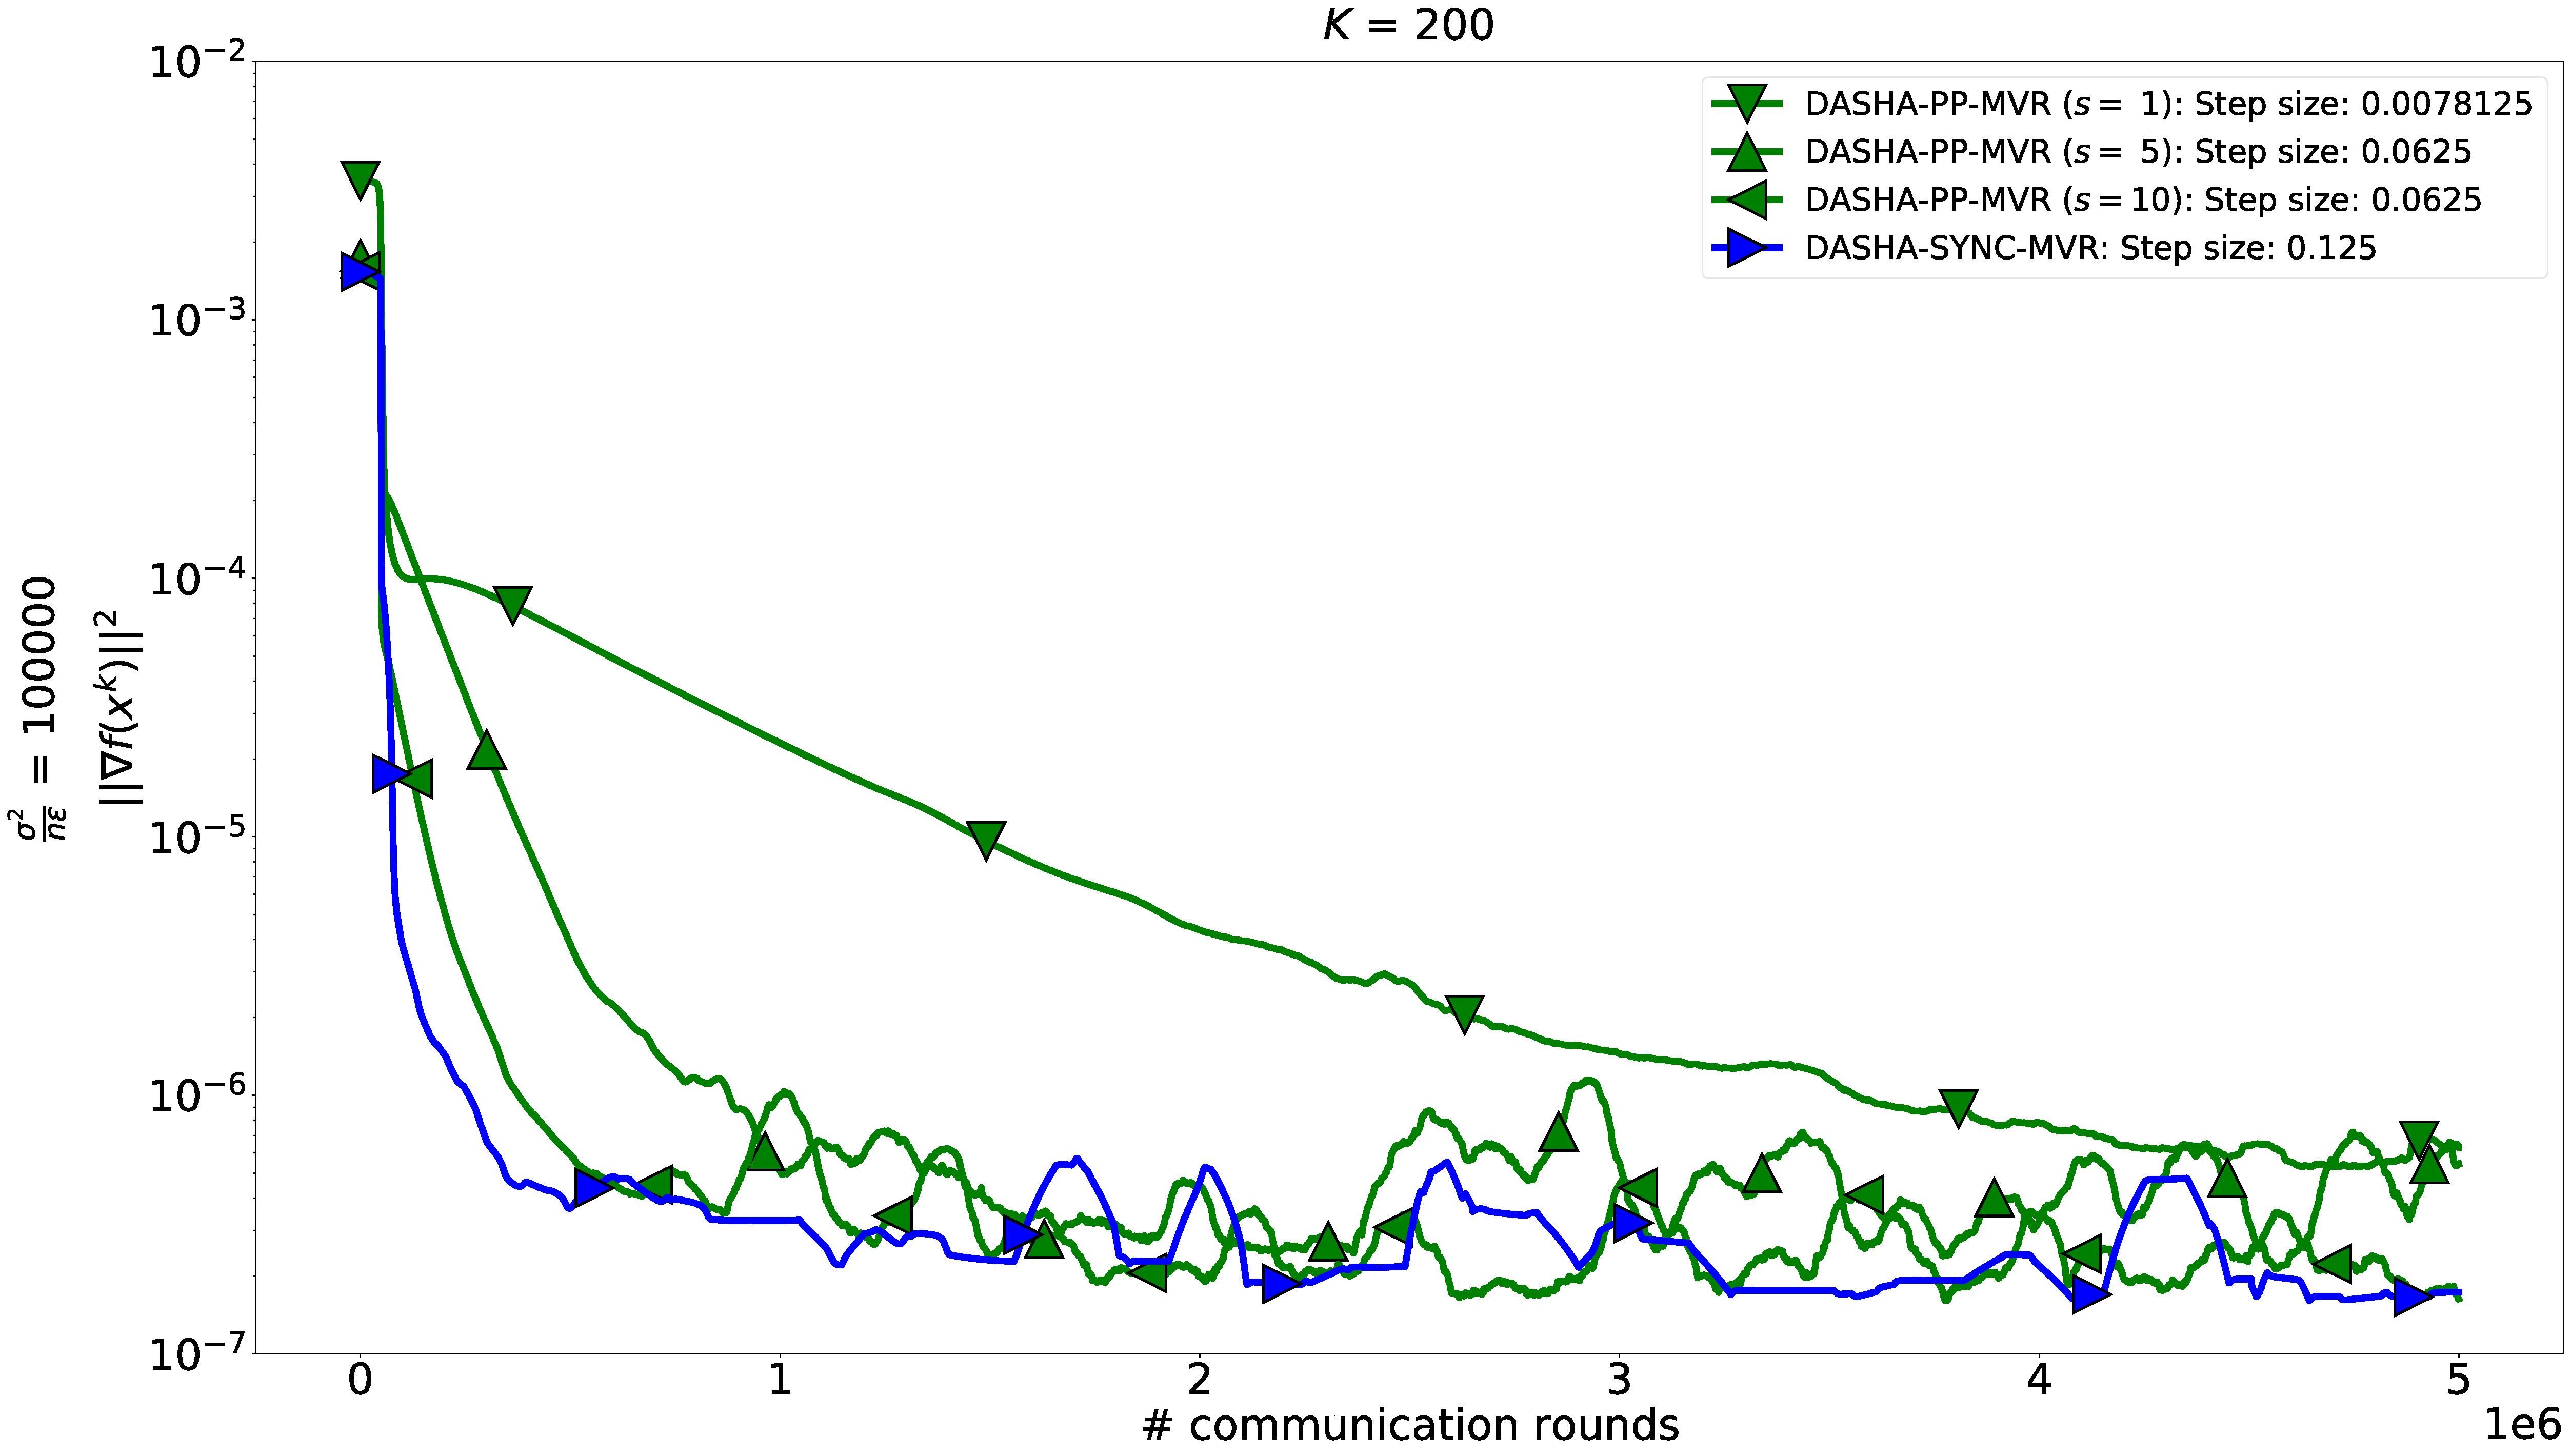
\includegraphics[width=0.75\linewidth]{experiments/neurips_2022_stochastic_real-sim_nof_200_numnodes_10_probs_mega_batch_100000_fix_nm_bug_longer.pdf}
%   \begin{tikzpicture}
%     \node[anchor=south west,inner sep=0] at (0,0) {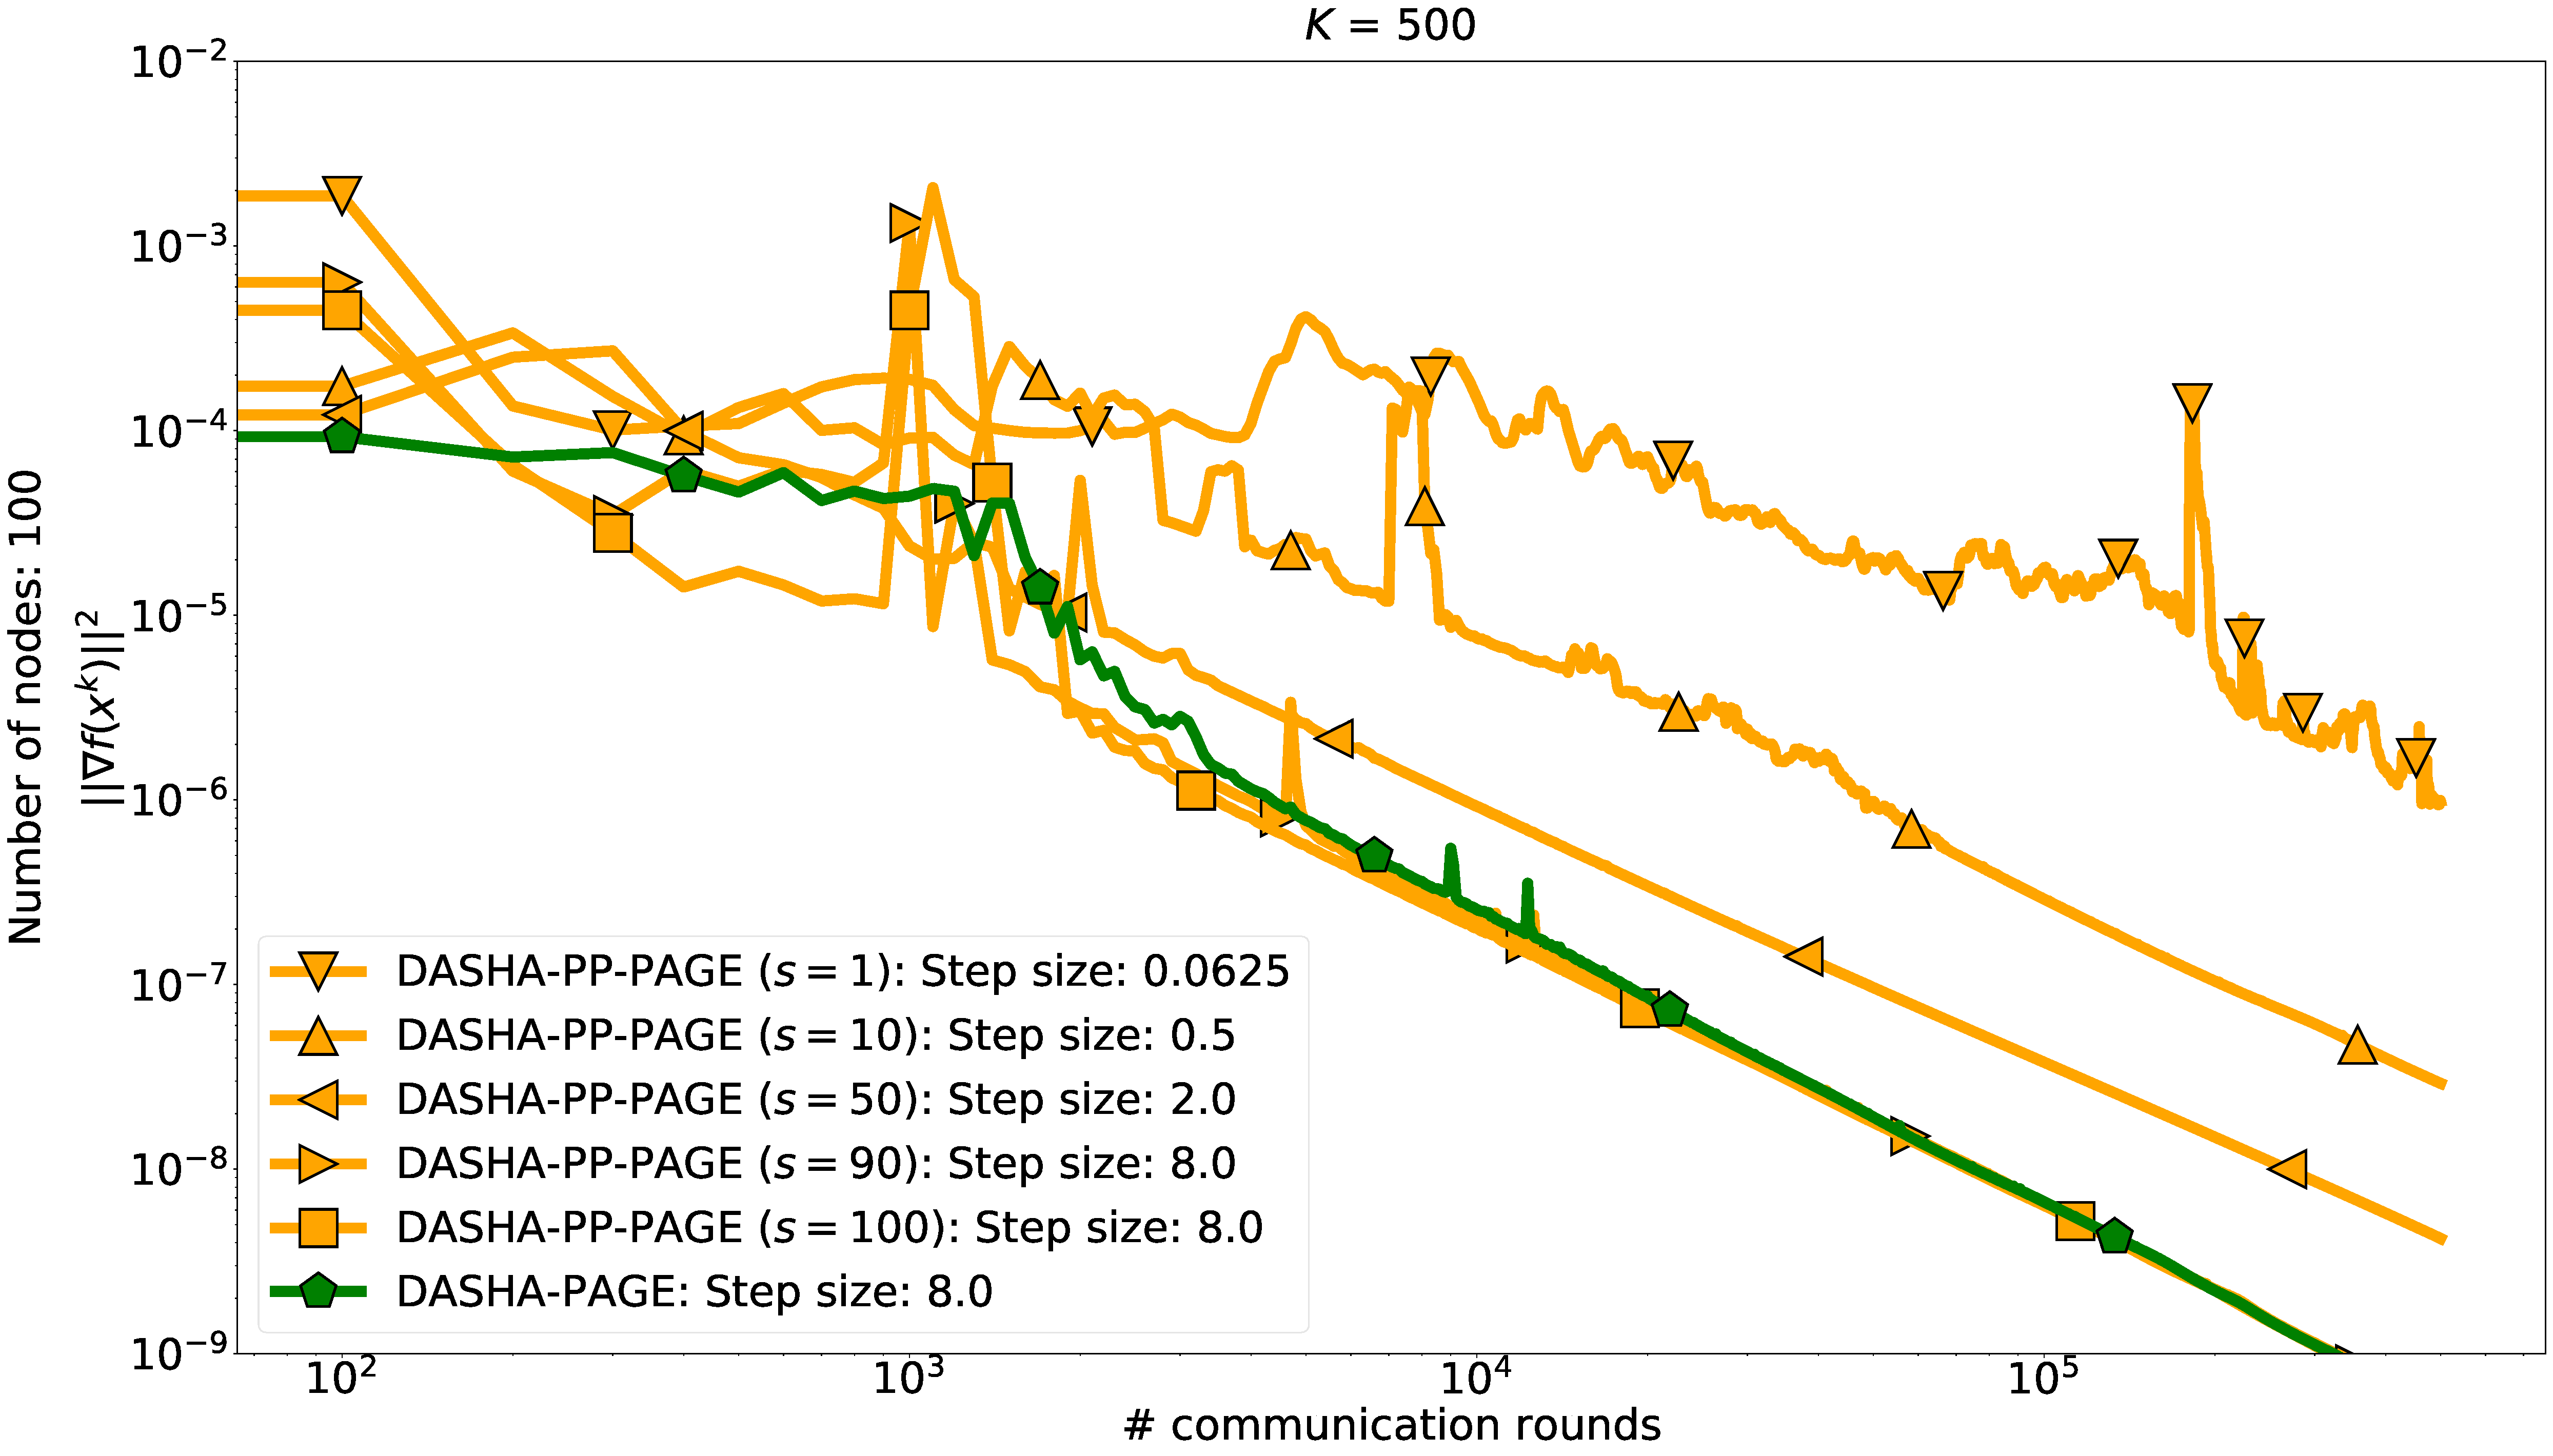
\includegraphics[width=\textwidth]{experiments/neurips_2022_finite_sum_real-sim_nof_500_numnodes_100_more_probs_batch_size_1_longer.pdf}};
%     \draw [black,ultra thick,decorate,decoration={brace,amplitude=20pt,raise=4ex}]
%       (7.0,3.0) -- (13.3,3.0) node[midway,yshift=+4.5em,xshift=+2em]{$\approx \times 100 \textnormal{ slower with } \probavailable = 0.01$};
%     \draw [black,ultra thick,decorate,decoration={brace,amplitude=20pt,raise=4ex}]
%       (9.8,1.5) -- (13.3,1.5) node[midway,yshift=+4.5em,xshift=+1em]{$\approx \times 10 \textnormal{ slower with } \probavailable = 0.1$};
%   \end{tikzpicture}
%   \caption{Classification task with the real-sim dataset, $K = 500$ in Rand$K$, in the finite-sum setting.}
%   \label{fig:real_sim_finite_sum}
% \end{figure}

% \begin{figure}[h]
%   \centering
%   % 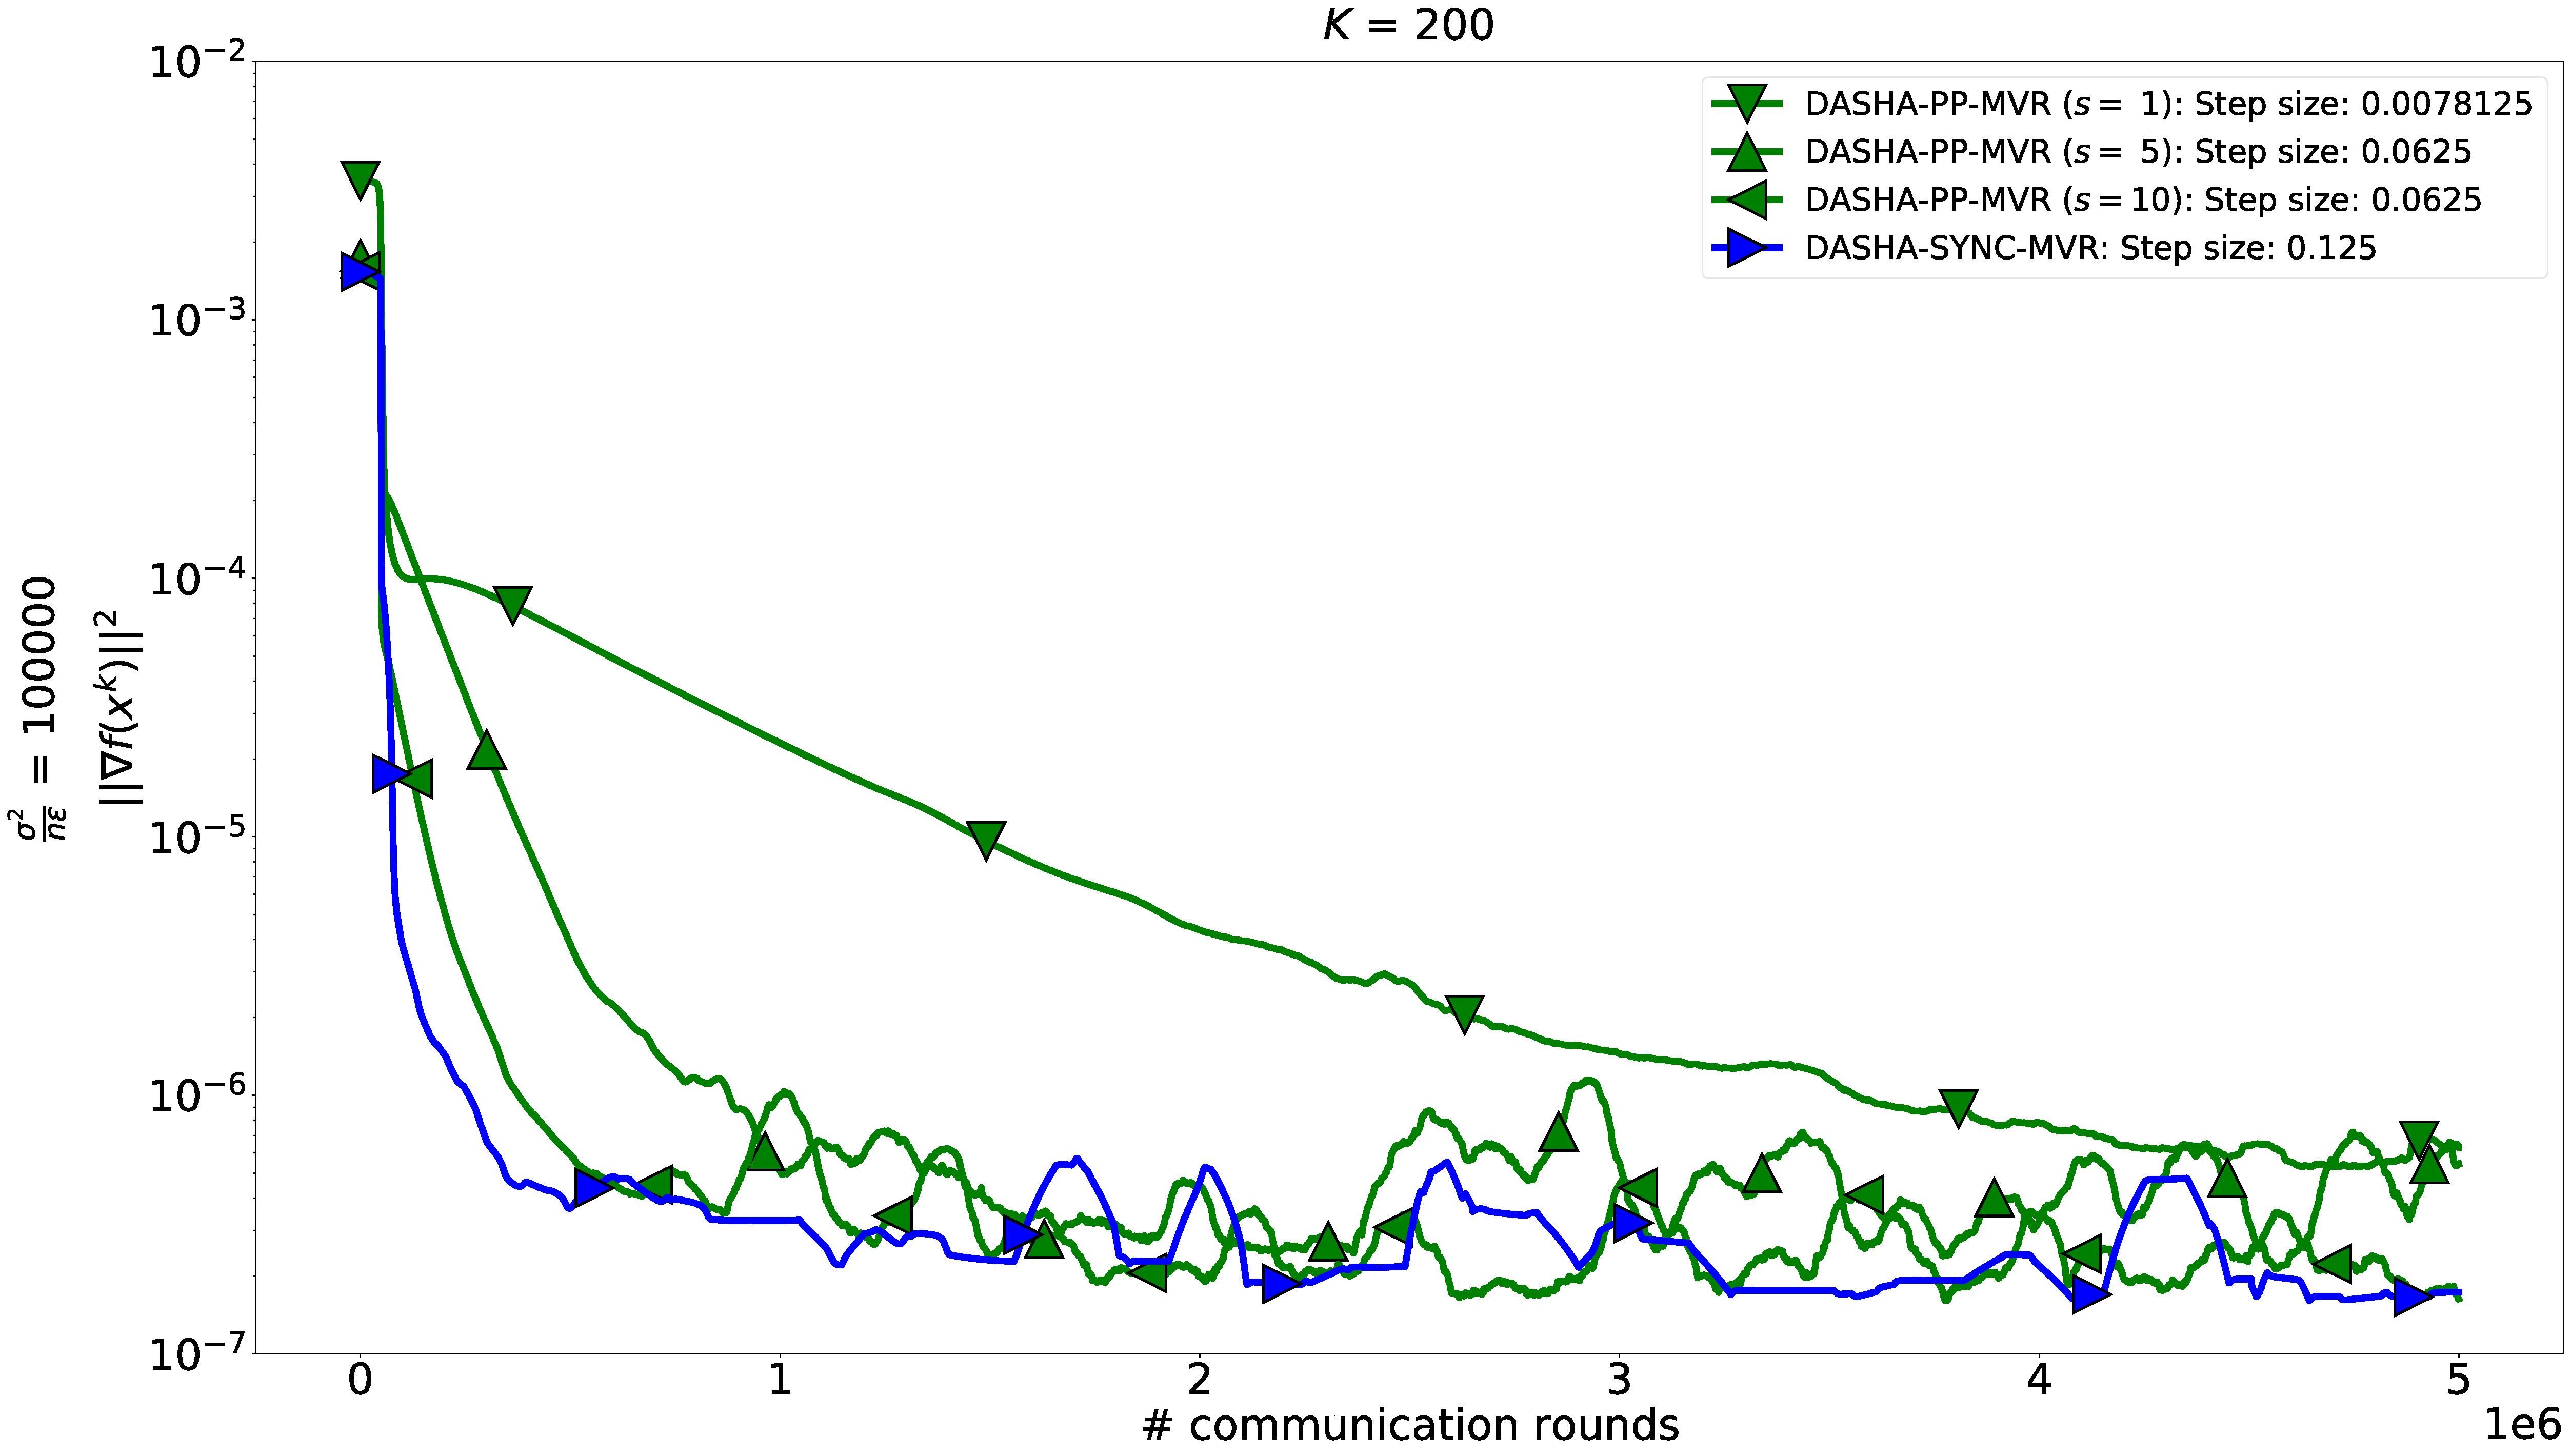
\includegraphics[width=0.75\linewidth]{experiments/neurips_2022_stochastic_real-sim_nof_200_numnodes_10_probs_mega_batch_100000_fix_nm_bug_longer.pdf}
%   \begin{tikzpicture}
%     \node[anchor=south west,inner sep=0] at (0,0) {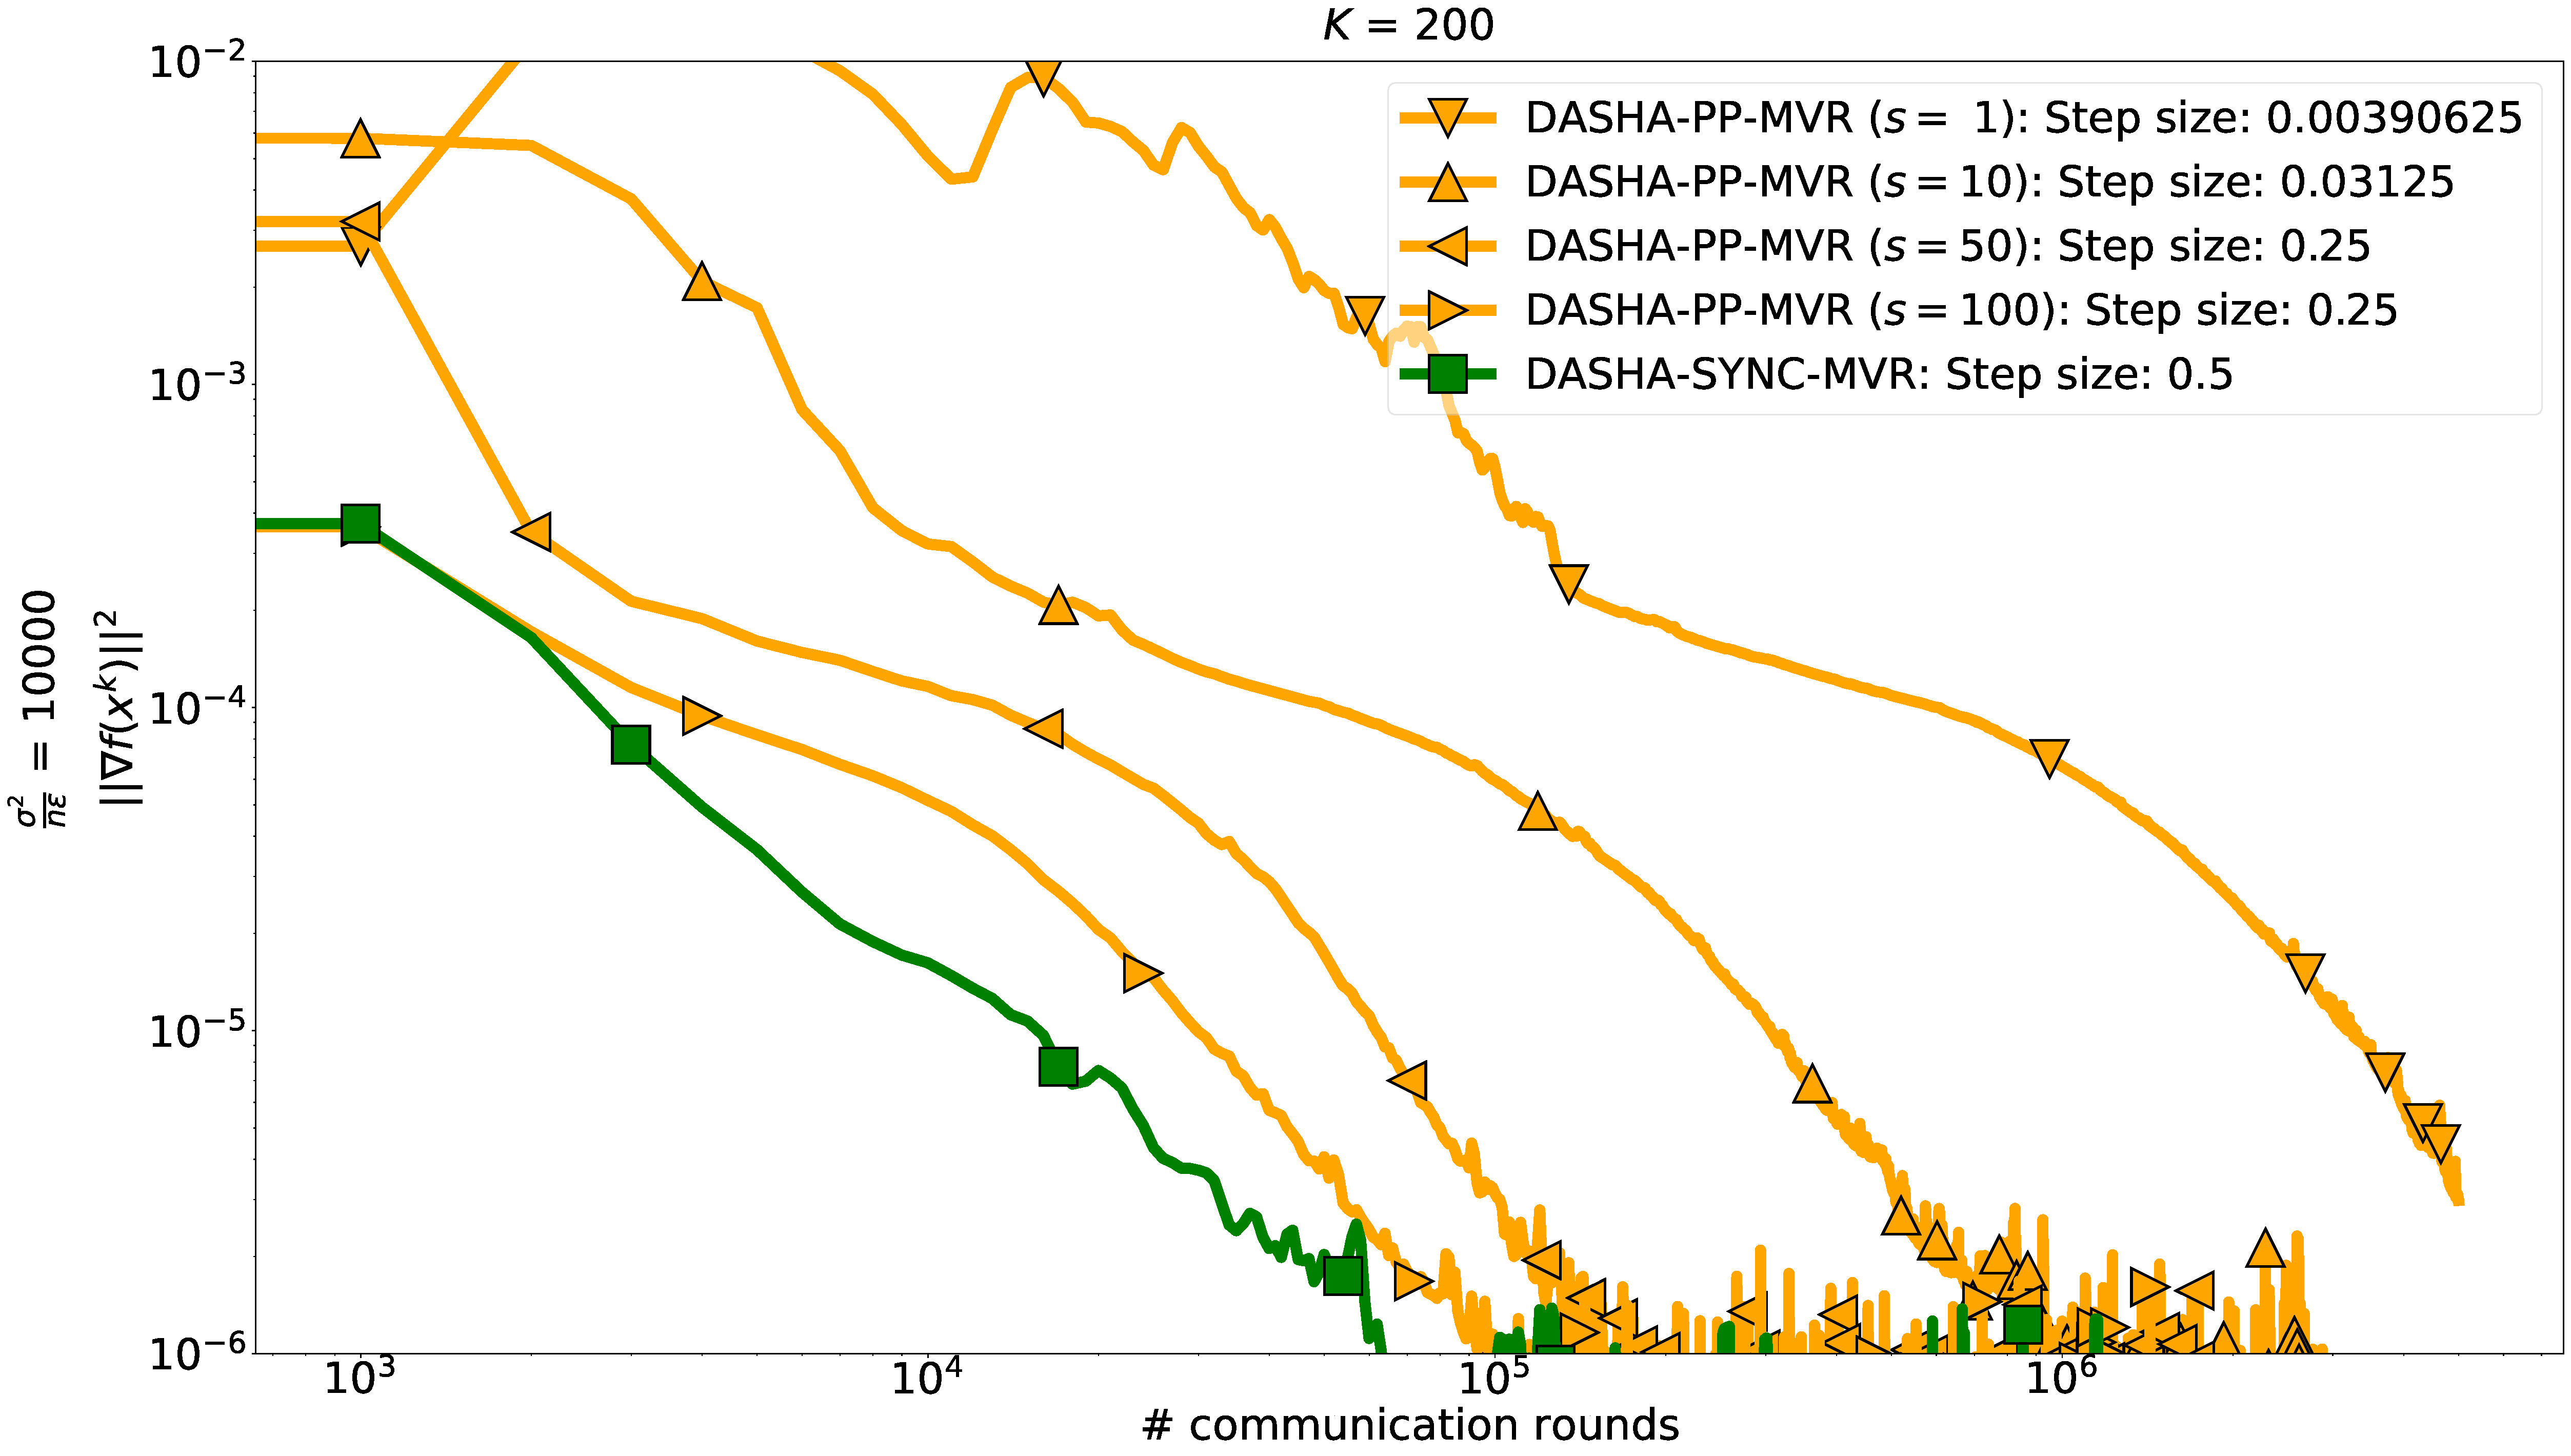
\includegraphics[width=\textwidth]{experiments/neurips_2022_stochastic_real-sim_nof_200_numnodes_100_probs_mega_batch_10000_fix_nm_bug_longer.pdf}};
%     \draw [black,ultra thick,decorate,decoration={brace,amplitude=20pt,raise=4ex}]
%       (7.3,0.8) -- (13.3,0.8) node[midway,yshift=+4.5em,xshift=+2em]{$\approx \times 100 \textnormal{ slower with } \probavailable = 0.01$};
%   \end{tikzpicture}
%   \caption{Classification task with the real-sim dataset, $\nicefrac{\sigma^2}{n \varepsilon B} = ?,$ and $K = 200$ in Rand$K$ in the stochastic setting.}
%   \label{fig:real_sim_stochastic}
% \end{figure}

\begin{figure}[h]
\centering
\begin{subfigure}{.5\textwidth}
  \centering
  \begin{tikzpicture}
    \node[anchor=south west,inner sep=0] at (0,0) {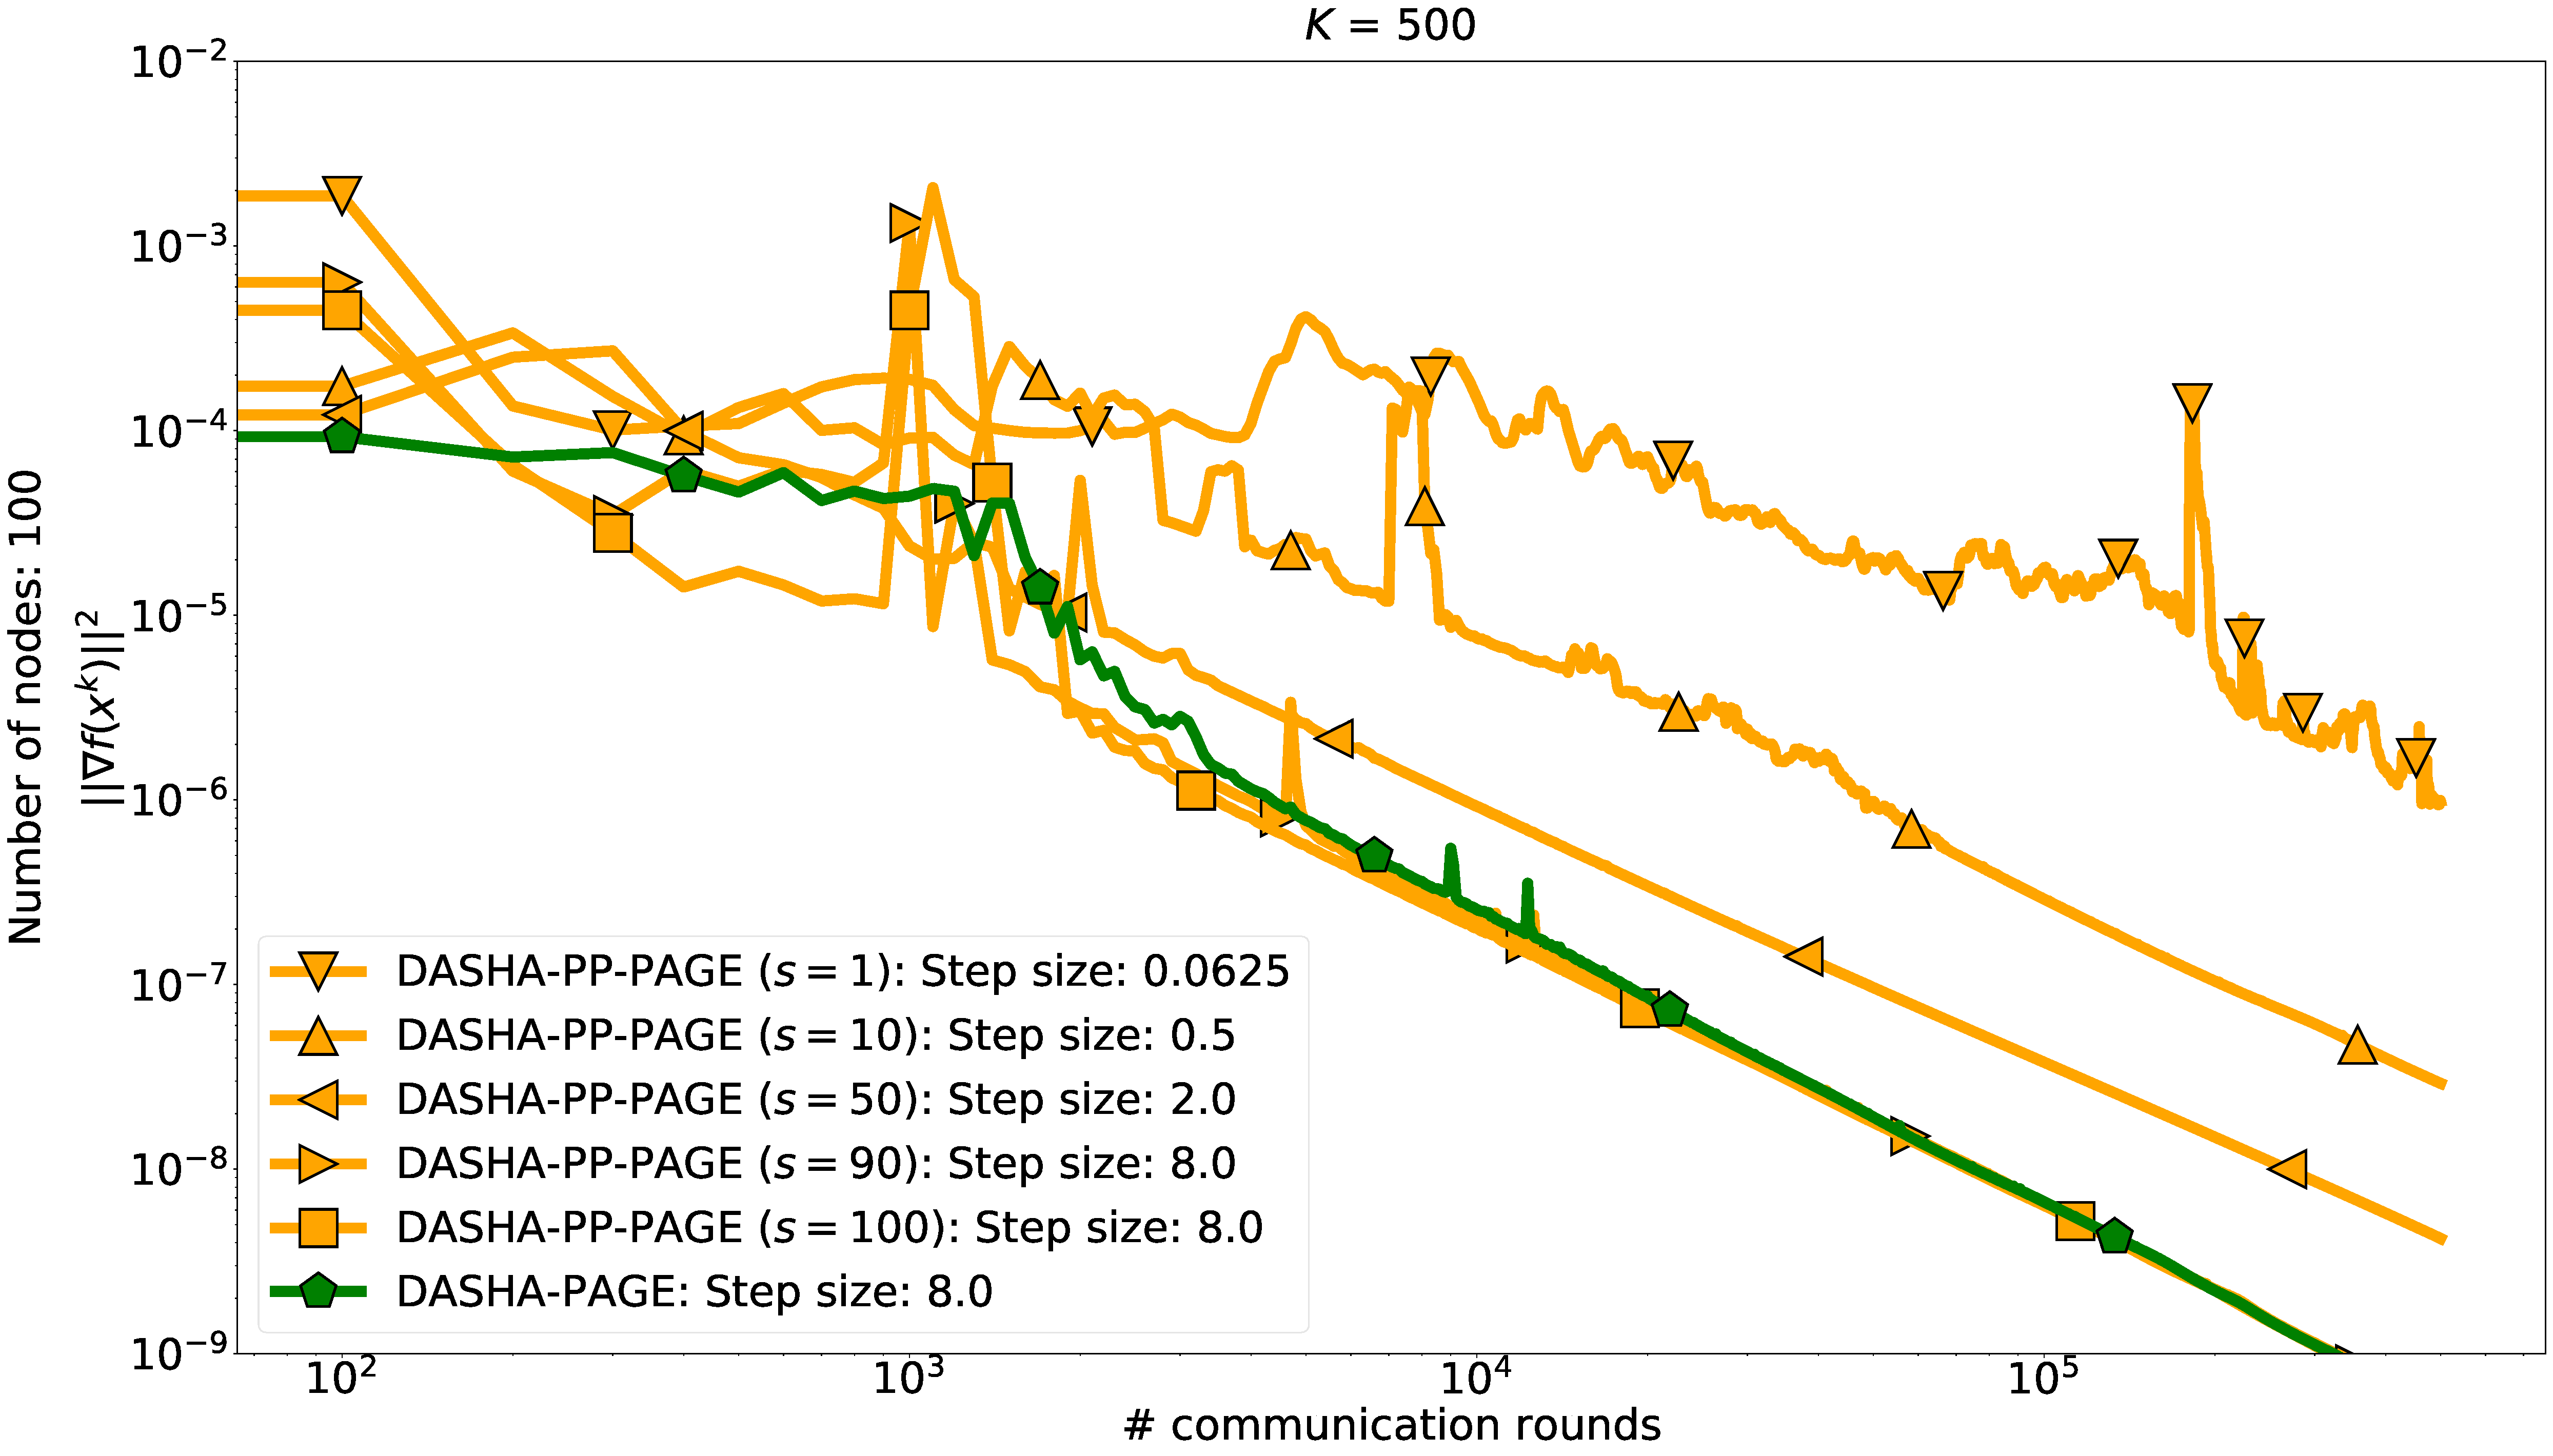
\includegraphics[width=\textwidth]{experiments/neurips_2022_finite_sum_real-sim_nof_500_numnodes_100_more_probs_batch_size_1_longer.pdf}};
    \draw [black,thick,<->] (3.6,1.8) -- (6.6,1.8) node[midway,yshift=-0.5em,xshift=+3.0em]{\scriptsize $\times 100 \textnormal{ slower}$};
    \draw [black,thick,<->] (5.1,1.0) -- (6.6,1.0) node[midway,yshift=-0.5em,xshift=-4.0em]{\scriptsize $\times 10 \textnormal{ slower}$};
    % \draw [black,ultra thick,decorate,decoration={brace,amplitude=20pt,raise=4ex}]
    %   (7.0,3.0) -- (13.3,3.0) node[midway,yshift=+4.5em,xshift=+2em]{$\approx \times 100 \textnormal{ slower with } \probavailable = 0.01$};
    % \draw [black,ultra thick,decorate,decoration={brace,amplitude=20pt,raise=4ex}]
    %   (9.8,1.5) -- (13.3,1.5) node[midway,yshift=+4.5em,xshift=+1em]{$\approx \times 10 \textnormal{ slower with } \probavailable = 0.1$};
  \end{tikzpicture}
  \caption{Finite-sum setting, $K = 500$ in Rand$K$.}
  \label{fig:real_sim_finite_sum}
\end{subfigure}\hfill
\begin{subfigure}{.5\textwidth}
  \centering
  \vspace{0.3cm}
  % 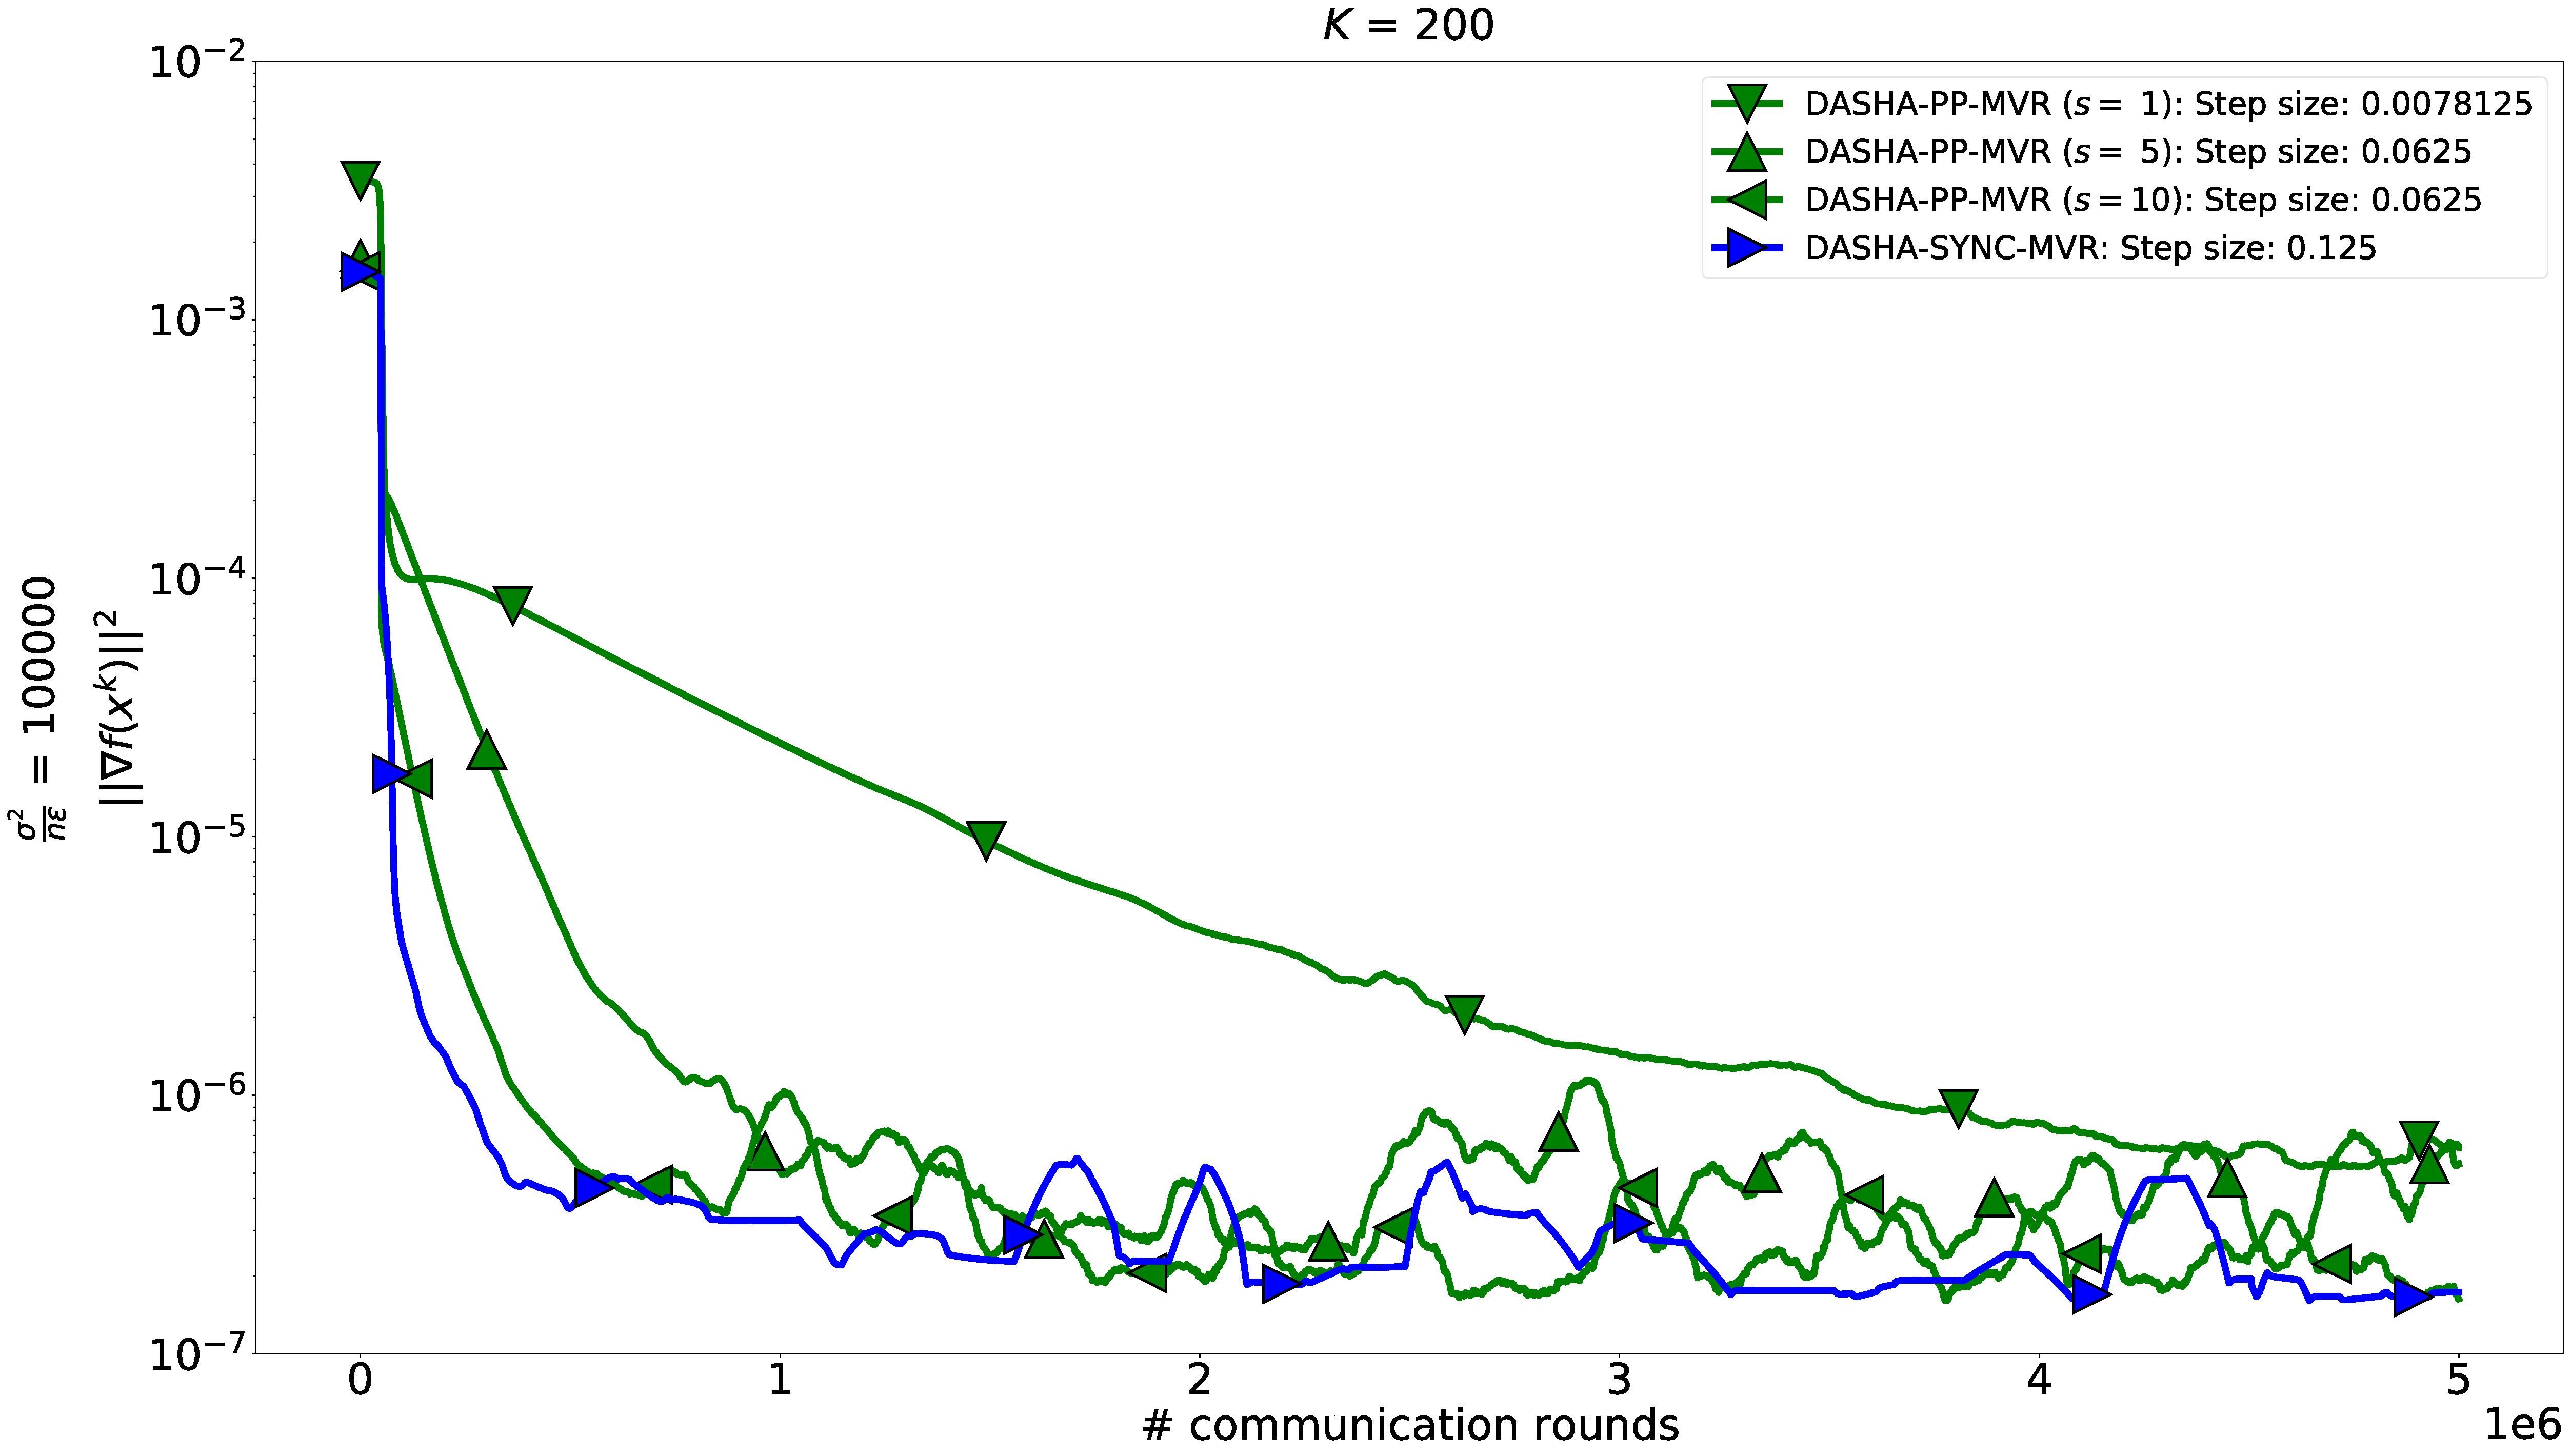
\includegraphics[width=0.75\linewidth]{experiments/neurips_2022_stochastic_real-sim_nof_200_numnodes_10_probs_mega_batch_100000_fix_nm_bug_longer.pdf}
  \begin{tikzpicture}
    \node[anchor=south west,inner sep=0] at (0,0) {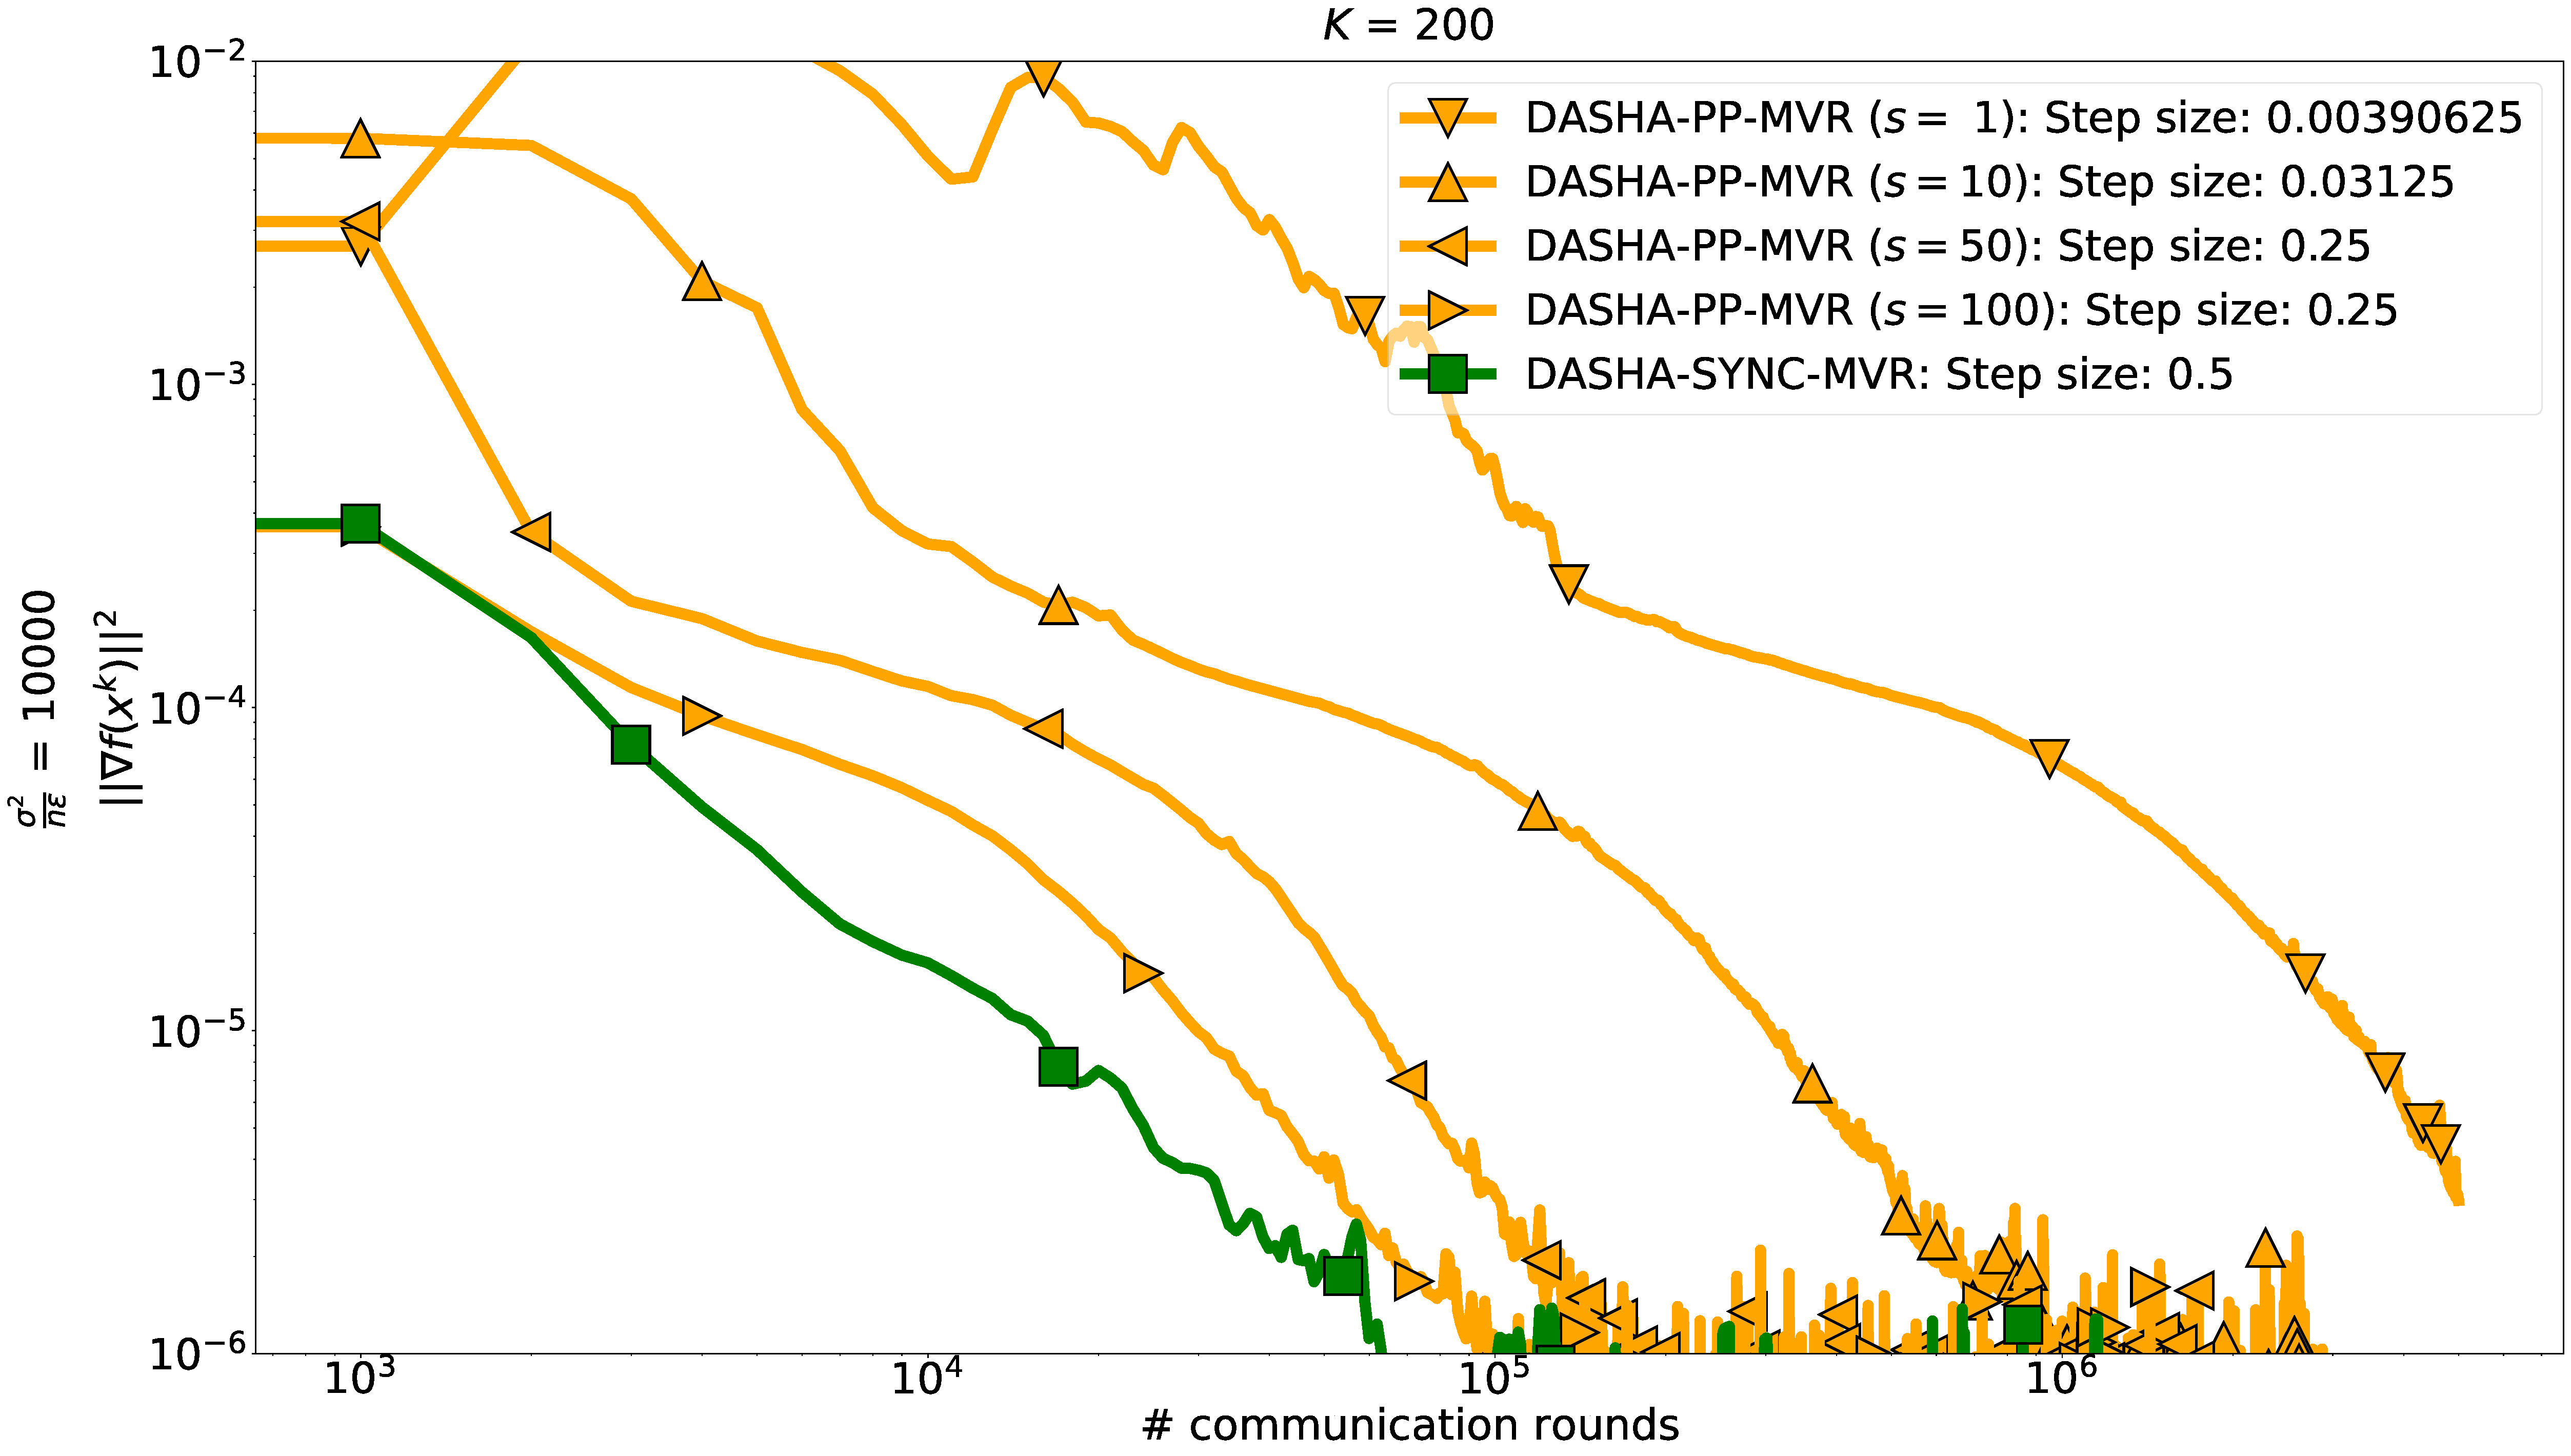
\includegraphics[width=\textwidth]{experiments/neurips_2022_stochastic_real-sim_nof_200_numnodes_100_probs_mega_batch_10000_fix_nm_bug_longer.pdf}};
    \draw [black,thick,<->] (3.7,0.7) -- (6.7,0.7) node[midway,yshift=+0.5em,xshift=+1.9em]{\scriptsize $\times 100 \textnormal{ slower}$};
    \draw [black,thick,<->] (3.7,0.8) -- (5.2,0.8) node[midway,yshift=+0.5em,xshift=+0.2em]{\scriptsize $\times 10 \textnormal{ slower}$};
    % \draw [black,ultra thick,decorate,decoration={brace,amplitude=20pt,raise=4ex}]
    %   (7.3,0.8) -- (13.3,0.8) node[midway,yshift=+4.5em,xshift=+2em]{$\approx \times 100 \textnormal{ slower with } \probavailable = 0.01$};
  \end{tikzpicture}
  \caption{Stochastic setting, $\nicefrac{\sigma^2}{n \varepsilon B} = 10000,$ and $K = 200$ in Rand$K$.}
  \label{fig:real_sim_stochastic}
\end{subfigure}
\caption{Classification task with the \textit{real-sim} dataset.}
\label{fig:test}
\end{figure}

\bibliographystyle{apalike}
\bibliography{neurips_2022}

\newpage
\appendix
\tableofcontents

\section{Auxiliary facts}
We list auxiliary facts that we use in our proofs:
\begin{enumerate}
    \item 
        For all $x, y \in \R^d,$ we have
        \begin{align}
            \norm{x + y}^2 \leq 2\norm{x}^2 + 2\norm{y}^2
            \label{auxiliary:jensen_inequality}
        \end{align}
    \item
        Let us take a \textit{random vector} $\xi \in \R^d$, then
        \begin{align}
            \Exp{\norm{\xi}^2} = \Exp{\norm{\xi - \Exp{\xi}}^2} + \norm{\Exp{\xi}}^2.
            \label{auxiliary:variance_decomposition}
        \end{align}
\end{enumerate}

\subsection{Sampling Lemma}
This section provides a lemma that we regularly use in our proofs, and it is useful for samplings that satisfy Assumption~\ref{ass:partial_participation}.
\begin{lemma}
  \label{lemma:sampling}
  Suppose that a set $S$ is a random subset of a set $[n]$ such that
  \begin{enumerate}
    \Item \begin{align*}\Prob\left(i \in S\right) = \probavailable, \quad \forall i \in [n],\end{align*}
    \Item \begin{align*}\Prob\left(i \in S, j \in S\right) = \probpairaa, \quad \forall i \neq j \in [n],\end{align*}
    \Item \begin{align*}
      \probpairaa \leq \probavailable^2,
    \end{align*}
  \end{enumerate}
  where $\probavailable \in (0, 1]$ and $\probpairaa \in [0, 1].$ Let us take random \textit{independent} vectors $s_i \in \R^d$ for all $i \in [n]$, nonrandom vector $r_i \in \R^d$ for all $i \in [n],$ and random vectors
  \begin{align*}
    v_i = \begin{cases}
      r_i + \frac{1}{\probavailable} s_i, i \in S, \\
      r_i, i \not\in S,
    \end{cases}
  \end{align*}
  then
  \begin{align*}
    &\Exp{\norm{\frac{1}{n}\sum_{i=1}^n v_i - \Exp{\frac{1}{n}\sum_{i=1}^n v_i}}^2} \\
    &= \frac{1}{n^2 \probavailable}\sum_{i=1}^n\Exp{\norm{s_i - \Exp{s_i}}^2} +\frac{\probavailable - \probpairaa}{n^2 \probavailable^2}\sum_{i=1}^n\norm{\Exp{s_i}}^2 + \frac{\probpairaa - \probavailable^2}{\probavailable^2}\norm{\frac{1}{n}\sum_{i=1}^n\Exp{s_i}}\\
    &\leq \frac{1}{n^2 \probavailable}\sum_{i=1}^n\Exp{\norm{s_i - \Exp{s_i}}^2} +\frac{\probavailable - \probpairaa}{n^2 \probavailable^2}\sum_{i=1}^n\norm{\Exp{s_i}}^2.
  \end{align*}
\end{lemma}

\begin{proof}
  Let us define additional constants $\probpairan$ and $\probpairnn$, such that
  \begin{enumerate}
    \Item \begin{align*}\Prob\left(i \in S, j \not\in S\right) = \probpairan, \quad \forall i \neq j \in [n],\end{align*}
    \Item \begin{align*}\Prob\left(i \not\in S, j \not\in S\right) = \probpairnn, \quad \forall i \neq j \in [n].\end{align*}
  \end{enumerate}
  Note, that 
  \begin{align}
    \label{auxiliary_facts_partial_participation:one}
    \probpairan = \probpairaa - \probavailable
  \end{align}
  and 
  \begin{align}
    \label{auxiliary_facts_partial_participation:two}
    \probpairnn = 1 - \probpairaa - 2 \probpairan.
  \end{align}
  Using the law of total expectation and 
  \begin{align*}
    \Exp{v_i} = \probavailable \left(r_i + \Exp{\frac{1}{\probavailable} s_i}\right) + (1 - \probavailable) r_i = r_i + \Exp{s_i},
  \end{align*}
  we have
  \begin{align*}
    &\Exp{\norm{\frac{1}{n}\sum_{i=1}^n v_i - \Exp{\frac{1}{n}\sum_{i=1}^n v_i}}^2} \\
    &=\frac{1}{n^2}\sum_{i=1}^n\Exp{\norm{v_i - \left(r_i + \Exp{s_i}\right)}^2} \\
    &\quad +\frac{1}{n^2}\sum_{i\neq j}^n\Exp{\inp{v_i - \left(r_i + \Exp{s_i}\right)}{v_j - \left(r_j + \Exp{s_j}\right)}} \\
    &=\frac{\probavailable}{n^2}\sum_{i=1}^n\Exp{\norm{r_i + \frac{1}{\probavailable} s_i - \left(r_i + \Exp{s_i}\right)}^2} \\
    &\quad +\frac{1 - \probavailable}{n^2}\sum_{i=1}^n\norm{r_i - \left(r_i + \Exp{s_i}\right)}^2 \\
    &\quad +\frac{\probpairaa}{n^2}\sum_{i\neq j}^n\Exp{\inp{r_i + \frac{1}{\probavailable} s_i - \left(r_i + \Exp{s_i}\right)}{r_j + \frac{1}{\probavailable} s_j - \left(r_j + \Exp{s_j}\right)}} \\
    &\quad +\frac{2 \probpairan}{n^2}\sum_{i\neq j}^n\Exp{\inp{r_i + \frac{1}{\probavailable} s_i - \left(r_i + \Exp{s_i}\right)}{r_j - \left(r_j + \Exp{s_j}\right)}} \\
    &\quad +\frac{\probpairnn}{n^2}\sum_{i\neq j}^n\inp{r_i - \left(r_i + \Exp{s_i}\right)}{r_j - \left(r_j + \Exp{s_j}\right)}.
  \end{align*}
  From the independence of random vectors $s_i$, we obtain
  \begin{align*}
    &\Exp{\norm{\frac{1}{n}\sum_{i=1}^n v_i - \Exp{\frac{1}{n}\sum_{i=1}^n v_i}}^2} \\
    &=\frac{\probavailable}{n^2}\sum_{i=1}^n\Exp{\norm{\frac{1}{\probavailable} s_i - \Exp{s_i}}^2} \\
    &\quad +\frac{1 - \probavailable}{n^2}\sum_{i=1}^n\norm{\Exp{s_i}}^2 \\
    &\quad +\frac{\probpairaa (1 - \probavailable)^2}{n^2 \probavailable^2}\sum_{i\neq j}^n\inp{\Exp{s_i}}{\Exp{s_j}} \\
    &\quad +\frac{2 \probpairan (\probavailable - 1)}{n^2 \probavailable}\sum_{i\neq j}^n\inp{\Exp{s_i}}{\Exp{s_j}} \\
    &\quad +\frac{\probpairnn}{n^2}\sum_{i\neq j}^n\inp{\Exp{s_i}}{\Exp{s_j}}.
  \end{align*}
  Using \eqref{auxiliary_facts_partial_participation:one} and \eqref{auxiliary_facts_partial_participation:two}, we have
  \begin{align*}
    &\Exp{\norm{\frac{1}{n}\sum_{i=1}^n v_i - \Exp{\frac{1}{n}\sum_{i=1}^n v_i}}^2} \\
    &=\frac{\probavailable}{n^2}\sum_{i=1}^n\Exp{\norm{\frac{1}{\probavailable} s_i - \Exp{s_i}}^2} \\
    &\quad +\frac{1 - \probavailable}{n^2}\sum_{i=1}^n\norm{\Exp{s_i}}^2 \\
    &\quad +\frac{\probpairaa - \probavailable^2}{n^2 \probavailable^2}\sum_{i\neq j}^n\inp{\Exp{s_i}}{\Exp{s_j}} \\
    &\overset{\eqref{auxiliary:variance_decomposition}}{=}\frac{1}{n^2 \probavailable}\sum_{i=1}^n\Exp{\norm{s_i - \Exp{s_i}}^2} \\
    &\quad +\frac{1 - \probavailable}{n^2 \probavailable}\sum_{i=1}^n\norm{\Exp{s_i}}^2 \\
    &\quad +\frac{\probpairaa - \probavailable^2}{n^2 \probavailable^2}\sum_{i\neq j}^n\inp{\Exp{s_i}}{\Exp{s_j}} \\
    &=\frac{1}{n^2 \probavailable}\sum_{i=1}^n\Exp{\norm{s_i - \Exp{s_i}}^2} \\
    &\quad +\frac{\probavailable - \probpairaa}{n^2 \probavailable^2}\sum_{i=1}^n\norm{\Exp{s_i}}^2 \\
    &\quad +\frac{\probpairaa - \probavailable^2}{\probavailable^2}\norm{\frac{1}{n}\sum_{i=1}^n\Exp{s_i}}.
  \end{align*}
  Finally, using that $\probpairaa \leq \probavailable^2$, we have
  \begin{align*}
    &\Exp{\norm{\frac{1}{n}\sum_{i=1}^n v_i - \Exp{\frac{1}{n}\sum_{i=1}^n v_i}}^2} \\
    &\leq\frac{1}{n^2 \probavailable}\sum_{i=1}^n\Exp{\norm{s_i - \Exp{s_i}}^2} +\frac{\probavailable - \probpairaa}{n^2 \probavailable^2}\sum_{i=1}^n\norm{\Exp{s_i}}^2.
  \end{align*}
\end{proof}

\subsection{Compressors Facts}

We define the Rand$K$ compressor that chooses without replacement $K$ coordinates, scales them by a constant factor to preserve unbiasedness and zero-out other coordinates.
\begin{definition}
    \label{def:rand_k}
    Let us take a random subset $S$ from $[d],$ $|S| = K,$ $K \in [d].$ We say that a stochastic mapping $\cC\,:\, \R^d \rightarrow \R^d$ is Rand$K$ if
    $$\cC(x) = \frac{d}{K} \sum_{j \in S} x_j e_j,$$ where $\{e_i\}_{i=1}^d$ is the standard unit basis.
\end{definition}

\begin{theorem}
    \label{theorem:rand_k}
    If $\cC$ is Rand$K$, then $\cC \in \mathbb{U}\left(\frac{d}{k} - 1\right).$
\end{theorem}
See the proof in \cite{beznosikov2020biased}.

\section{Proofs of Theorems}
\label{sec:proof_of_theorems}

There are three different sources of randomness in Algorithm~\ref{alg:main_algorithm}: the first one from vectors $\{k_i^{t+1}\}_{i=1}^n$, the second one from compressors $\{\cC_i\}_{i=1}^n$, and the third one from availability of nodes. We define $\ExpSub{k}{\cdot}$, $\ExpSub{\cC}{\cdot}$ and $\ExpSub{\probavailable}{\cdot}$ to be conditional expectations w.r.t.\,$\{k_i^{t+1}\}_{i=1}^n$, $\{\cC_i\}_{i=1}^n, $ and availability, accordingly, conditioned on all previous randomness. Moreover, we define $\ExpSub{t+1}{\cdot}$ to be a conditional expectation w.r.t. all randomness in iteration $t+1$ conditioned on all previous randomness. Note, that $\ExpSub{t+1}{\cdot} = \ExpSub{k}{\ExpSub{\cC}{\ExpSub{\probavailable}{\cdot}}}.$

In the case of \algname{\algorithmname-PAGE}, there are two different sources of randomness from $\{k_i^{t+1}\}_{i=1}^n$. We define $\ExpSub{\probpage}{\cdot}$ and $\ExpSub{B}{\cdot}$ to be conditional expectations w.r.t.\, the probabilistic switching and mini-batch indices $I_{i}^t$, accordingly, conditioned on all previous randomness. Note, that $\ExpSub{t+1}{\cdot} = \ExpSub{B}{\ExpSub{\cC}{\ExpSub{\probavailable}{\ExpSub{\probpage}{\cdot}}}}$ and $\ExpSub{t+1}{\cdot} = \ExpSub{B}{\ExpSub{\probpage}{\ExpSub{\cC}{\ExpSub{\probavailable}{\cdot}}}}.$

\subsection{Standard Lemmas in the Nonconvex Setting}

We start the proof of theorems by providing standard lemmas from the nonconvex optimization.

\begin{lemma}
  \label{lemma:page_lemma}
  Suppose that Assumption~\ref{ass:lipschitz_constant} holds and let $x^{t+1} = x^{t} - \gamma g^{t}$. Then for any $g^{t} \in \R^d$ and $\gamma > 0$, we have
  \begin{eqnarray}
    \label{eq:page_lemma}
    f(x^{t + 1}) \leq f(x^t) - \frac{\gamma}{2}\norm{\nabla f(x^t)}^2 - \left(\frac{1}{2\gamma} - \frac{L}{2}\right)
    \norm{x^{t+1} - x^t}^2 + \frac{\gamma}{2}\norm{g^{t} - \nabla f(x^t)}^2.
  \end{eqnarray}
\end{lemma}

\begin{proof}
  Using $L-$smoothness, we have 
  \begin{align*}
    f(x^{t+1}) &\leq f(x^t) + \inp{\nabla f(x^t)}{x^{t+1} - x^{t}} + \frac{L}{2} \norm{x^{t+1} - x^{t}}^2 \\
    &= f(x^t) - \gamma \inp{\nabla f(x^t)}{g^t} + \frac{L}{2} \norm{x^{t+1} - x^{t}}^2.
  \end{align*}
  Next, due to $-\inp{x}{y} = \frac{1}{2}\norm{x - y}^2 - \frac{1}{2}\norm{x}^2 - \frac{1}{2}\norm{y}^2,$ we obtain 
  \begin{align*}
    f(x^{t+1}) \leq f(x^t) -\frac{\gamma}{2} \norm{\nabla f(x^t)}^2 - \left(\frac{1}{2\gamma} - \frac{L}{2}\right) \norm{x^{t+1} - x^{t}}^2 + \frac{\gamma}{2}\norm{g^t - \nabla f(x^t)}^2.
  \end{align*}
\end{proof}

\begin{lemma}
  \label{lemma:good_recursion}
  Suppose that Assumption \ref{ass:lower_bound} holds and
  \begin{align*}
      \Exp{f(x^{t+1})} + \gamma \Psi^{t+1} \leq \Exp{f(x^t)} - \frac{\gamma}{2}\Exp{\norm{\nabla f(x^t)}^2} + \gamma \Psi^{t} + \gamma C,
  \end{align*}
  where $\Psi^{t}$ is a sequence of numbers, $\Psi^{t} \geq 0$ for all $t \in [T]$, constant $C \geq 0$, and constant $\gamma > 0.$ Then 
  \begin{align}
      \label{eq:good_recursion}
      \Exp{\norm{\nabla f(\widehat{x}^T)}^2} \leq \frac{2 \Delta_0}{\gamma T} + \frac{2\Psi^{0}}{T} + 2 C,
  \end{align}
  where a point $\widehat{x}^T$ is chosen uniformly from a set of points $\{x^t\}_{t=0}^{T-1}.$
\end{lemma}

\begin{proof}
  By unrolling \eqref{eq:good_recursion} for $t$ from $0$ to $T - 1$, we obtain
  \begin{align*}
      \frac{\gamma}{2}\sum_{t = 0}^{T - 1}\Exp{\norm{\nabla f(x^t)}^2} + \Exp{f(x^{T})} + \gamma \Psi^{T} \leq f(x^0) + \gamma \Psi^{0} + \gamma T C.
  \end{align*}
  We subtract $f^*$, divide inequality by $\frac{\gamma T}{2},$ and take into account that $f(x) \geq f^*$ for all $x \in \R$, and $\Psi^{t} \geq 0$ for all $t \in [T],$ to get the following inequality:
  \begin{align*}
      \frac{1}{T}\sum_{t = 0}^{T - 1}\Exp{\norm{\nabla f(x^t)}^2} \leq \frac{2 \Delta_0}{\gamma T} + \frac{2\Psi^{0}}{T} + 2 C.
  \end{align*}
  It is left to consider the choice of a point $\widehat{x}^T$ to complete the proof of the lemma.
\end{proof}

\begin{lemma}
  \label{lemma:gamma}
  If $0 < \gamma \leq (L + \sqrt{A})^{-1},$ $L > 0$, and $A \geq 0,$ then $$\frac{1}{2\gamma} - \frac{L}{2} - \frac{\gamma A}{2} \geq 0.$$
\end{lemma}
The lemma can be easily checked with the direct calculation.

\subsection{Generic Lemmas}
\begin{lemma}
  Suppose that Assumptions~\ref{ass:compressors} and \ref{ass:partial_participation} hold and let us consider sequences $g^{t+1}_i$, $h^{t+1}_i,$ and $k^{t+1}_i$ from Algorithm~\ref{alg:main_algorithm}, then
  \begin{align}
      \label{eq:compressor_global_error}
      &\ExpSub{\cC}{\ExpSub{\probavailable}{\norm{g^{t+1} - h^{t+1}}^2}} \nonumber \\
      &\leq \frac{2 \omega}{n^2 \probavailable}\sum_{i=1}^n\norm{k^{t+1}_i}^2 +\frac{a^2 (\left(2 \omega + 1\right)\probavailable - \probpairaa)}{n^2 \probavailable^2}\sum_{i=1}^n\norm{g^{t}_i - h^{t}_i}^2 + (1 - a)^2\norm{g^{t} - h^{t}}^2,
  \end{align}
  and
  \begin{align}
      \label{eq:compressor_local_error}
      &\ExpSub{\cC}{\ExpSub{\probavailable}{\norm{g^{t+1}_i - h^{t+1}_i}^2}} \nonumber \\
      &\leq \frac{2 \omega}{\probavailable}\norm{k^{t+1}_i}^2 + \left(\frac{a^2(2\omega + 1 - \probavailable)}{\probavailable} + (1 - a)^2\right)\norm{g^{t}_i - h^{t}_i}^2\quad \forall i \in [n].
  \end{align}
\end{lemma}
\begin{proof}
  First, we estimate $\ExpSub{\cC}{\ExpSub{\probavailable}{\norm{g^{t+1} - h^{t+1}}^2}}$:
  \begin{align*}
      &\ExpSub{\cC}{\ExpSub{\probavailable}{\norm{g^{t+1} - h^{t+1}}^2}} \\
      &=\ExpSub{\cC}{\ExpSub{\probavailable}{\norm{g^{t+1} - h^{t+1} - \ExpSub{\cC}{\ExpSub{\probavailable}{g^{t+1} - h^{t+1}}}}^2}} + \norm{\ExpSub{\cC}{\ExpSub{\probavailable}{g^{t+1} - h^{t+1}}}}^2,
  \end{align*}
  where we used \eqref{auxiliary:variance_decomposition}.
  Due to Assumption~\ref{ass:partial_participation}, we have
  \begin{align*}
      &\ExpSub{\cC}{\ExpSub{\probavailable}{g^{t+1}_i}} \\
      &=\probavailable \ExpSub{\cC}{g^{t}_i + \cC_i\Bigg(\frac{1}{\probavailable}k^{t+1}_i - \frac{a}{\probavailable} \left(g^{t}_i - h^{t}_i\right)\Bigg)} + (1 - \probavailable) g^{t}_i \\
      &=g^{t}_i  + \probavailable\ExpSub{\cC}{\cC_i\Bigg(\frac{1}{\probavailable}k^{t+1}_i - \frac{a}{\probavailable} \left(g^{t}_i - h^{t}_i\right)\Bigg)} \\
      &=g^{t}_i  + k^{t+1}_i - a \left(g^{t}_i - h^{t}_i\right), \\
  \end{align*}
  and 
  \begin{align*}
      &\ExpSub{\cC}{\ExpSub{\probavailable}{h^{t+1}_i}} = \probavailable \ExpSub{\cC}{h^t_i + \frac{1}{\probavailable}k^{t+1}_i} + (1 - \probavailable) h^{t}_i = h^{t}_i + k^{t+1}_i. \\
  \end{align*}
  Thus, we can get
  \begin{align*}
      &\ExpSub{\cC}{\ExpSub{\probavailable}{\norm{g^{t+1} - h^{t+1}}^2}} \\
      &=\ExpSub{\cC}{\ExpSub{\probavailable}{\norm{g^{t+1} - h^{t+1} - \ExpSub{\cC}{\ExpSub{\probavailable}{g^{t+1} - h^{t+1}}}}^2}} + (1 - a)^2\norm{g^{t} - h^{t}}^2.
  \end{align*}
  Due to the independence of compressors, we can use Lemma~\ref{lemma:sampling} with $r_i = g^{t}_i - h^{t}_i$ and $s_i = \probavailable\cC_i\Bigg(\frac{1}{\probavailable}k^{t+1}_i - \frac{a}{\probavailable} \left(g^{t}_i - h^{t}_i\right)\Bigg) - k^{t+1}_i,$ and obtain
  \begin{align*}
    &\ExpSub{\cC}{\ExpSub{\probavailable}{\norm{g^{t+1} - h^{t+1}}^2}} \\
    &\leq \frac{1}{n^2 \probavailable}\sum_{i=1}^n\ExpSub{\cC}{\norm{\probavailable\cC_i\Bigg(\frac{1}{\probavailable}k^{t+1}_i - \frac{a}{\probavailable} \left(g^{t}_i - h^{t}_i\right)\Bigg) - k^{t+1}_i - \ExpSub{\cC}{\probavailable\cC_i\Bigg(\frac{1}{\probavailable}k^{t+1}_i - \frac{a}{\probavailable} \left(g^{t}_i - h^{t}_i\right)\Bigg) - k^{t+1}_i}}^2} \\
    &\quad +\frac{\probavailable - \probpairaa}{n^2 \probavailable^2}\sum_{i=1}^n\norm{\ExpSub{\cC}{\probavailable\cC_i\Bigg(\frac{1}{\probavailable}k^{t+1}_i - \frac{a}{\probavailable} \left(g^{t}_i - h^{t}_i\right)\Bigg) - k^{t+1}_i}}^2 \\
    &\quad + (1 - a)^2\norm{g^{t} - h^{t}}^2 \\
    &= \frac{\probavailable}{n^2}\sum_{i=1}^n\ExpSub{\cC}{\norm{\cC_i\Bigg(\frac{1}{\probavailable}k^{t+1}_i - \frac{a}{\probavailable} \left(g^{t}_i - h^{t}_i\right)\Bigg) - \Bigg(\frac{1}{\probavailable}k^{t+1}_i - \frac{a}{\probavailable} \left(g^{t}_i - h^{t}_i\right)\Bigg)}^2} \\
    &\quad +\frac{a^2 \left(\probavailable - \probpairaa\right)}{n^2 \probavailable^2}\sum_{i=1}^n\norm{g^{t}_i - h^{t}_i}^2 + (1 - a)^2\norm{g^{t} - h^{t}}^2.
  \end{align*}
  From Assumption~\ref{ass:compressors}, we have
  \begin{align*}
    &\ExpSub{\cC}{\ExpSub{\probavailable}{\norm{g^{t+1} - h^{t+1}}^2}} \\
    &\leq \frac{\omega \probavailable}{n^2}\sum_{i=1}^n\norm{\frac{1}{\probavailable}k^{t+1}_i - \frac{a}{\probavailable} \left(g^{t}_i - h^{t}_i\right)}^2 +\frac{a^2 \left(\probavailable - \probpairaa\right)}{n^2 \probavailable^2}\sum_{i=1}^n\norm{g^{t}_i - h^{t}_i}^2 + (1 - a)^2\norm{g^{t} - h^{t}}^2 \\
    &= \frac{\omega}{n^2 \probavailable}\sum_{i=1}^n\norm{k^{t+1}_i - a \left(g^{t}_i - h^{t}_i\right)}^2 +\frac{a^2 \left(\probavailable - \probpairaa\right)}{n^2 \probavailable^2}\sum_{i=1}^n\norm{g^{t}_i - h^{t}_i}^2 + (1 - a)^2\norm{g^{t} - h^{t}}^2 \\
    &\overset{\eqref{auxiliary:jensen_inequality}}{\leq} \frac{2 \omega}{n^2 \probavailable}\sum_{i=1}^n\norm{k^{t+1}_i}^2 +\frac{a^2 \left((2\omega + 1)\probavailable - \probpairaa\right)}{n^2 \probavailable^2}\sum_{i=1}^n\norm{g^{t}_i - h^{t}_i}^2 + (1 - a)^2\norm{g^{t} - h^{t}}^2.
  \end{align*}
  The second inequality can be proved almost in the same way:
  \begin{align*}
    &\ExpSub{\cC}{\ExpSub{\probavailable}{\norm{g^{t+1}_i - h^{t+1}_i}^2}} \\
    &=\ExpSub{\cC}{\ExpSub{\probavailable}{\norm{g^{t+1}_i - h^{t+1}_i - \ExpSub{\cC}{\ExpSub{\probavailable}{g^{t+1}_i - h^{t+1}_i}}}^2}} + \norm{\ExpSub{\cC}{\ExpSub{\probavailable}{g^{t+1}_i - h^{t+1}_i}}}^2 \\
    &=\ExpSub{\cC}{\ExpSub{\probavailable}{\norm{g^{t+1}_i - h^{t+1}_i - g^{t}_i + a \left(g^{t}_i - h^{t}_i\right) + h^{t}_i}^2}} + (1 - a)^2\norm{g^{t}_i - h^{t}_i}^2 \\
    &=\probavailable\ExpSub{\cC}{\norm{\cC_i\Bigg(\frac{1}{\probavailable}k^{t+1}_i - \frac{a}{\probavailable} \left(g^{t}_i - h^{t}_i\right)\Bigg) - \frac{1}{\probavailable}k^{t+1}_i + a \left(g^{t}_i - h^{t}_i\right)}^2} \\
    &\quad + a^2(1 - \probavailable)\norm{g^{t}_i - h^{t}_i}^2 + (1 - a)^2\norm{g^{t}_i - h^{t}_i}^2 \\
    &\overset{\eqref{auxiliary:variance_decomposition}}{=}\probavailable\ExpSub{\cC}{\norm{\cC_i\Bigg(\frac{1}{\probavailable}k^{t+1}_i - \frac{a}{\probavailable} \left(g^{t}_i - h^{t}_i\right)\Bigg) - \left(\frac{1}{\probavailable}k^{t+1}_i - \frac{a}{\probavailable} \left(g^{t}_i - h^{t}_i\right)\right)}^2} \\
    &\quad + a^2 \frac{(1 - \probavailable)^2}{\probavailable} \norm{g^{t}_i - h^{t}_i}^2 \\
    &\quad + a^2(1 - \probavailable)\norm{g^{t}_i - h^{t}_i}^2 + (1 - a)^2\norm{g^{t}_i - h^{t}_i}^2 \\
    &\leq \frac{\omega}{\probavailable}\norm{k^{t+1}_i - a \left(g^{t}_i - h^{t}_i\right)}^2 \\
    &\quad + \frac{a^2(1 - \probavailable)}{\probavailable} \norm{g^{t}_i - h^{t}_i}^2 + (1 - a)^2\norm{g^{t}_i - h^{t}_i}^2 \\
    &\overset{\eqref{auxiliary:jensen_inequality}}{\leq} \frac{2 \omega}{\probavailable}\norm{k^{t+1}_i}^2 + \frac{a^2(2\omega + 1 - \probavailable)}{\probavailable} \norm{g^{t}_i - h^{t}_i}^2 + (1 - a)^2\norm{g^{t}_i - h^{t}_i}^2.
  \end{align*}
\end{proof}

\begin{lemma}
  \label{lemma:main_lemma}
  Suppose that Assumptions \ref{ass:lipschitz_constant}, \ref{ass:compressors}, and \ref{ass:partial_participation} hold and let us take $a = \frac{\probavailable}{2 \omega + 1},$ then
  \begin{align*}
    &\Exp{f(x^{t + 1})} + \frac{\gamma (2 \omega + 1)}{\probavailable} \Exp{\norm{g^{t+1} - h^{t+1}}^2} + \frac{\gamma (\left(2 \omega + 1\right)\probavailable - \probpairaa)}{n \probavailable^2} \Exp{\frac{1}{n}\sum_{i=1}^n\norm{g^{t+1}_i - h^{t+1}_i}^2}\\
    &\leq \Exp{f(x^t) - \frac{\gamma}{2}\norm{\nabla f(x^t)}^2 - \left(\frac{1}{2\gamma} - \frac{L}{2}\right)
    \norm{x^{t+1} - x^t}^2 + \gamma \norm{h^{t} - \nabla f(x^t)}^2}\nonumber\\
    &\quad + \frac{\gamma (2 \omega + 1)}{\probavailable}\Exp{\norm{g^{t} - h^t}^2}+ \frac{\gamma (\left(2 \omega + 1\right)\probavailable - \probpairaa)}{n \probavailable^2}\Exp{\frac{1}{n} \sum_{i=1}^n\norm{g^t_i - h^{t}_i}^2} + \frac{4 \gamma \omega (2 \omega + 1)}{n \probavailable^2} \Exp{\frac{1}{n} \sum_{i=1}^n\norm{k^{t+1}_i}^2}.
  \end{align*}
\end{lemma}

\begin{proof}
  Due to Lemma \ref{lemma:page_lemma} and the update step from Line~\ref{alg:main_algorithm:x_update} in Algorithm~\ref{alg:main_algorithm}, we have
  \begin{align*}
    &\ExpSub{t+1}{f(x^{t + 1})} \nonumber\\
    &\leq \ExpSub{t+1}{f(x^t) - \frac{\gamma}{2}\norm{\nabla f(x^t)}^2 - \left(\frac{1}{2\gamma} - \frac{L}{2}\right)
      \norm{x^{t+1} - x^t}^2 + \frac{\gamma}{2}\norm{g^{t} - \nabla f(x^t)}^2} \nonumber \\
      &= \ExpSub{t+1}{f(x^t) - \frac{\gamma}{2}\norm{\nabla f(x^t)}^2 - \left(\frac{1}{2\gamma} - \frac{L}{2}\right)
      \norm{x^{t+1} - x^t}^2 + \frac{\gamma}{2}\norm{g^{t} - h^t + h^t - \nabla f(x^t)}^2} \nonumber \\
      &\overset{\eqref{auxiliary:variance_decomposition}}{\leq} \ExpSub{t+1}{f(x^t) - \frac{\gamma}{2}\norm{\nabla f(x^t)}^2 - \left(\frac{1}{2\gamma} - \frac{L}{2}\right)
      \norm{x^{t+1} - x^t}^2 + \gamma\left(\norm{g^{t} - h^t}^2 + \norm{h^t - \nabla f(x^t)}^2}\right). \nonumber \\
      \nonumber
  \end{align*}
  Let us fix some constants $\kappa, \eta \in [0,\infty)$ that we will define later. Combining the last inequality, bounds \eqref{eq:compressor_global_error}, \eqref{eq:compressor_local_error} and using the law of total expectation, we get
  \begin{align*}
      &\Exp{f(x^{t + 1})} \nonumber \\
      &\quad  + \kappa \Exp{\norm{g^{t+1} - h^{t+1}}^2} + \eta \Exp{\frac{1}{n}\sum_{i=1}^n\norm{g^{t+1}_i - h^{t+1}_i}^2} \nonumber\\
      &=\Exp{\ExpSub{t+1}{f(x^{t + 1})}} \nonumber \\
      &\quad  + \kappa \Exp{\ExpSub{\cC}{\ExpSub{\probavailable}{\norm{g^{t+1} - h^{t+1}}^2}}} + \eta \Exp{\ExpSub{\cC}{\ExpSub{\probavailable}{\frac{1}{n}\sum_{i=1}^n\norm{g^{t+1}_i - h^{t+1}_i}^2}}} \nonumber\\
      &\leq \Exp{f(x^t) - \frac{\gamma}{2}\norm{\nabla f(x^t)}^2 - \left(\frac{1}{2\gamma} - \frac{L}{2}\right)
      \norm{x^{t+1} - x^t}^2 + \gamma\left(\norm{g^{t} - h^t}^2 + \norm{h^{t} - \nabla f(x^t)}^2\right)} \nonumber\\
      &\quad +\kappa \Exp{\frac{2 \omega}{n^2 \probavailable}\sum_{i=1}^n\norm{k^{t+1}_i}^2 +\frac{a^2 (\left(2 \omega + 1\right)\probavailable - \probpairaa)}{n^2 \probavailable^2}\sum_{i=1}^n\norm{g^{t}_i - h^{t}_i}^2 + (1 - a)^2\norm{g^{t} - h^{t}}^2} \nonumber\\
      &\quad +\eta \Exp{\frac{2 \omega}{n \probavailable} \sum_{i=1}^n \norm{k^{t+1}_i}^2 + \left(\frac{a^2(2\omega + 1 - \probavailable)}{\probavailable} + (1 - a)^2\right)\frac{1}{n}\sum_{i=1}^n\norm{g^{t}_i - h^{t}_i}^2} \\
      &= \Exp{f(x^t) - \frac{\gamma}{2}\norm{\nabla f(x^t)}^2 - \left(\frac{1}{2\gamma} - \frac{L}{2}\right)
      \norm{x^{t+1} - x^t}^2 + \gamma \norm{h^{t} - \nabla f(x^t)}^2}\nonumber\\
      &\quad + \left(\gamma + \kappa \left(1 - a\right)^2\right)\Exp{\norm{g^{t} - h^t}^2}\nonumber\\
      &\quad + \left(\frac{\kappa a^2 (\left(2 \omega + 1\right)\probavailable - \probpairaa)}{n \probavailable^2} + \eta\left(\frac{a^2(2\omega + 1 - \probavailable)}{\probavailable} + (1 - a)^2\right)\right)\Exp{\frac{1}{n} \sum_{i=1}^n\norm{g^t_i - h^{t}_i}^2}\nonumber\\
      &\quad + \left(\frac{2 \kappa \omega}{n \probavailable} + \frac{2 \eta \omega}{\probavailable}\right)\Exp{\frac{1}{n} \sum_{i=1}^n\norm{k^{t+1}_i}^2}.
  \end{align*}
  Now, by taking $\kappa = \frac{\gamma}{a}$, we can see that $\gamma + \kappa \left(1 - a\right)^2 \leq \kappa, $ and thus
  \begin{align*}
      &\Exp{f(x^{t + 1})} \\
      &\quad  + \frac{\gamma}{a} \Exp{\norm{g^{t+1} - h^{t+1}}^2} + \eta \Exp{\frac{1}{n}\sum_{i=1}^n\norm{g^{t+1}_i - h^{t+1}_i}^2}\\
      &\leq \Exp{f(x^t) - \frac{\gamma}{2}\norm{\nabla f(x^t)}^2 - \left(\frac{1}{2\gamma} - \frac{L}{2}\right)
      \norm{x^{t+1} - x^t}^2 + \gamma \norm{h^{t} - \nabla f(x^t)}^2}\nonumber\\
      &\quad + \frac{\gamma}{a}\Exp{\norm{g^{t} - h^t}^2}\nonumber\\
      &\quad + \left(\frac{\gamma a (\left(2 \omega + 1\right)\probavailable - \probpairaa)}{n \probavailable^2} + \eta\left(\frac{a^2(2\omega + 1 - \probavailable)}{\probavailable} + (1 - a)^2\right)\right)\Exp{\frac{1}{n} \sum_{i=1}^n\norm{g^t_i - h^{t}_i}^2}\nonumber\\
      &\quad + \left(\frac{2 \gamma \omega}{a n \probavailable} + \frac{2 \eta \omega}{\probavailable}\right)\Exp{\frac{1}{n} \sum_{i=1}^n\norm{k^{t+1}_i}^2}.
  \end{align*}
  Next, by taking $\eta = \frac{\gamma (\left(2 \omega + 1\right)\probavailable - \probpairaa)}{n \probavailable^2}$ and considering the choice of $a$, one can show that $\left(\frac{\gamma a (\left(2 \omega + 1\right)\probavailable - \probpairaa)}{n \probavailable^2} + \eta\left(\frac{a^2(2\omega + 1 - \probavailable)}{\probavailable} + (1 - a)^2\right)\right) \leq \eta.$ Thus

  \begin{align*}
    &\Exp{f(x^{t + 1})} \\
    &\quad  + \frac{\gamma (2 \omega + 1)}{\probavailable} \Exp{\norm{g^{t+1} - h^{t+1}}^2} + \frac{\gamma (\left(2 \omega + 1\right)\probavailable - \probpairaa)}{n \probavailable^2} \Exp{\frac{1}{n}\sum_{i=1}^n\norm{g^{t+1}_i - h^{t+1}_i}^2}\\
    &\leq \Exp{f(x^t) - \frac{\gamma}{2}\norm{\nabla f(x^t)}^2 - \left(\frac{1}{2\gamma} - \frac{L}{2}\right)
    \norm{x^{t+1} - x^t}^2 + \gamma \norm{h^{t} - \nabla f(x^t)}^2}\nonumber\\
    &\quad + \frac{\gamma (2 \omega + 1)}{\probavailable}\Exp{\norm{g^{t} - h^t}^2}+ \frac{\gamma (\left(2 \omega + 1\right)\probavailable - \probpairaa)}{n \probavailable^2}\Exp{\frac{1}{n} \sum_{i=1}^n\norm{g^t_i - h^{t}_i}^2}\nonumber\\
    &\quad + \left(\frac{2 \gamma (2 \omega + 1)\omega}{n \probavailable^2} + \frac{2 \gamma (\left(2 \omega + 1\right)\probavailable - \probpairaa) \omega}{n \probavailable^3}\right)\Exp{\frac{1}{n} \sum_{i=1}^n\norm{k^{t+1}_i}^2}.
  \end{align*}
  Considering that $\probpairaa \geq 0,$ we can simplify the last term and get
  \begin{align*}
    &\Exp{f(x^{t + 1})} \\
    &\quad  + \frac{\gamma (2 \omega + 1)}{\probavailable} \Exp{\norm{g^{t+1} - h^{t+1}}^2} + \frac{\gamma (\left(2 \omega + 1\right)\probavailable - \probpairaa)}{n \probavailable^2} \Exp{\frac{1}{n}\sum_{i=1}^n\norm{g^{t+1}_i - h^{t+1}_i}^2}\\
    &\leq \Exp{f(x^t) - \frac{\gamma}{2}\norm{\nabla f(x^t)}^2 - \left(\frac{1}{2\gamma} - \frac{L}{2}\right)
    \norm{x^{t+1} - x^t}^2 + \gamma \norm{h^{t} - \nabla f(x^t)}^2}\nonumber\\
    &\quad + \frac{\gamma (2 \omega + 1)}{\probavailable}\Exp{\norm{g^{t} - h^t}^2}+ \frac{\gamma (\left(2 \omega + 1\right)\probavailable - \probpairaa)}{n \probavailable^2}\Exp{\frac{1}{n} \sum_{i=1}^n\norm{g^t_i - h^{t}_i}^2}\nonumber\\
    &\quad + \frac{4 \gamma (2 \omega + 1)\omega}{n \probavailable^2} \Exp{\frac{1}{n} \sum_{i=1}^n\norm{k^{t+1}_i}^2}.
  \end{align*}
\end{proof}

% In the following lemma, we provide a helpful observation about $k^{t+1}_i$.

% \begin{lemma}
%   \label{lemma:expectation_k_t}
%   Suppose that Assumptions \ref{}, \ref{} and \ref{} hold. For $k^{t+1}_i$ from Algorithm~\ref{alg:main_algorithm} we have
%   \begin{align*}
%       &\ExpSub{k}{k^{t+1}_i} = \nabla f_i(x^{t+1}) - \nabla f_i(x^{t}) - b(h^t_i - \nabla f_i(x^{t})).
%   \end{align*}
% \end{lemma}

% \begin{proof}
%   Clearly, the equality holds for \algname{\algorithmname}. Next, we show it for \algname{\algorithmname-PAGE}:
%   \begin{align*}
%     &\ExpSub{k}{k^{t+1}_i} \\
%     &= \probpage \left(\nabla f_i(x^{t+1}) - \nabla f_i(x^{t}) - \frac{b}{\probpage} \left(h^t_i - \nabla f_i(x^{t})\right)\right) \\
%     &\quad + (1 - \probpage) \ExpSub{k}{\frac{1}{B}\sum_{j \in I^t_i}\left(\nabla f_{ij}(x^{t+1}) - \nabla f_{ij}(x^{t})\right)} \\
%     &= \probpage \left(\nabla f_i(x^{t+1}) - \nabla f_i(x^{t}) - \frac{b}{\probpage} \left(h^t_i - \nabla f_i(x^{t})\right)\right) \\
%     &\quad + (1 - \probpage) \left(\nabla f_i(x^{t+1}) - \nabla f_i(x^{t})\right) \\
%     &= \nabla f_i(x^{t+1}) - \nabla f_i(x^{t}) - b \left(h^t_i - \nabla f_i(x^{t})\right).
% \end{align*}
% Finally, from the unbiasedness of stochastic gradients, the equality holds for \algname{\algorithmname-MVR}.
% \end{proof}

\subsection{Proof for \algname{\algorithmname}}

\begin{lemma}
  \label{lemma:gradient}
  Suppose that Assumptions~\ref{ass:nodes_lipschitz_constant} and \ref{ass:partial_participation} hold. For $h^{t+1}_i$ and $k^{t+1}_i$ from Algorithm~\ref{alg:main_algorithm} (\algname{\algorithmname}) we have
  \begin{enumerate}
  \item
      \begin{align*}
          &\ExpSub{\probavailable}{\norm{h^{t+1} - \nabla f(x^{t+1})}^2} \\
          & \leq \frac{2\left(\probavailable - \probpairaa\right)\widehat{L}^2}{n \probavailable^2} \norm{x^{t+1} - x^{t}}^2 + \frac{2 b^2 \left(\probavailable - \probpairaa\right)}{n^2 \probavailable^2} \sum_{i=1}^n \norm{h^t_i - \nabla f_i(x^{t})}^2 + \left(1 - b\right)^2 \norm{h^{t} - \nabla f(x^{t})}^2.
      \end{align*}
  \item
      \begin{align*}
          &\ExpSub{\probavailable}{\norm{h^{t+1}_i - \nabla f_i(x^{t+1})}^2} \\
          & \leq \frac{2(1 - \probavailable)}{\probavailable} L^2_i \norm{x^{t+1} - x^{t}}^2 + \left(\frac{2 b^2 (1 - \probavailable)}{\probavailable} + (1 - b)^2\right) \norm{h^{t}_i - \nabla f_i(x^{t})}^2, \quad \forall i \in [n].
      \end{align*}
  \item
      \begin{align*}
        &\norm{k^{t+1}_i}^2 \leq 2L^2_i\norm{x^{t+1} - x^{t}}^2 + 2b^2 \norm{h^t_i - \nabla f_i(x^{t})}^2, \quad \forall i \in [n].
      \end{align*}
  \end{enumerate}
\end{lemma}

\begin{proof}
  First, let us proof the bound for $\ExpSub{k}{\ExpSub{\probavailable}{\norm{h^{t+1} - \nabla f(x^{t+1})}^2}}$:
  \begin{align*}
      &\ExpSub{\probavailable}{\norm{h^{t+1} - \nabla f(x^{t+1})}^2} \\
      &=\ExpSub{\probavailable}{\norm{h^{t+1} - \ExpSub{\probavailable}{h^{t+1}}}^2} + \norm{\ExpSub{\probavailable}{h^{t+1}} - \nabla f(x^{t+1})}^2.
  \end{align*}
  Using
  \begin{align*}
      \ExpSub{\probavailable}{h^{t+1}_i} = h^{t}_i + \nabla f_i(x^{t+1}) - \nabla f_i(x^{t}) - b(h^t_i - \nabla f_i(x^{t}))
  \end{align*}
  and \eqref{auxiliary:variance_decomposition}, we have
  \begin{align*}
    &\ExpSub{\probavailable}{\norm{h^{t+1} - \nabla f(x^{t+1})}^2} \\
    &=\ExpSub{\probavailable}{\norm{h^{t+1} - \ExpSub{\probavailable}{h^{t+1}}}^2} + \left(1 - b\right)^2 \norm{h^{t} - \nabla f(x^{t})}^2.
  \end{align*}
  We can use Lemma~\ref{lemma:sampling} with $r_i = h^{t}_i$ and $s_i = k^{t+1}_i$ to obtain
  \begin{align*}
    &\ExpSub{\probavailable}{\norm{h^{t+1} - \nabla f(x^{t+1})}^2} \\
    &\leq \frac{1}{n^2 \probavailable}\sum_{i=1}^n\norm{k^{t+1}_i - k^{t+1}_i}^2 +\frac{\probavailable - \probpairaa}{n^2 \probavailable^2}\sum_{i=1}^n\norm{k^{t+1}_i}^2 + \left(1 - b\right)^2 \norm{h^{t} - \nabla f(x^{t})}^2\\
    &= \frac{\probavailable - \probpairaa}{n^2 \probavailable^2}\sum_{i=1}^n\norm{\nabla f_i(x^{t+1}) - \nabla f_i(x^{t}) - b \left(h^t_i - \nabla f_i(x^{t})\right)}^2 + \left(1 - b\right)^2 \norm{h^{t} - \nabla f(x^{t})}^2\\
    &\overset{\eqref{auxiliary:jensen_inequality}}{\leq} \frac{2\left(\probavailable - \probpairaa\right)}{n^2 \probavailable^2}\sum_{i=1}^n\norm{\nabla f_i(x^{t+1}) - \nabla f_i(x^{t})}^2 + \frac{2 b^2 \left(\probavailable - \probpairaa\right)}{n^2 \probavailable^2}\sum_{i=1}^n\norm{h^t_i - \nabla f_i(x^{t})}^2 + \left(1 - b\right)^2 \norm{h^{t} - \nabla f(x^{t})}^2\\
    &\leq \frac{2\left(\probavailable - \probpairaa\right)\widehat{L}^2}{n \probavailable^2} \norm{x^{t+1} - x^{t}}^2 + \frac{2 b^2 \left(\probavailable - \probpairaa\right)}{n^2 \probavailable^2}\sum_{i=1}^n\norm{h^t_i - \nabla f_i(x^{t})}^2 + \left(1 - b\right)^2 \norm{h^{t} - \nabla f(x^{t})}^2.
  \end{align*}
  In the last in inequality, we used Assumption~\ref{ass:nodes_lipschitz_constant}. Now, we prove the second inequality:
  \begin{align*}
    &\ExpSub{\probavailable}{\norm{h^{t+1}_i - \nabla f_i(x^{t+1})}^2} \\
    &=\ExpSub{\probavailable}{\norm{h^{t+1}_i - \ExpSub{\probavailable}{h^{t+1}_i}}^2} + \norm{\ExpSub{\probavailable}{h^{t+1}_i  } - \nabla f_i(x^{t+1})}^2 \\
    &=\ExpSub{\probavailable}{\norm{h^{t+1}_i - \left(h^{t}_i + \nabla f_i(x^{t+1}) - \nabla f_i(x^{t}) - b(h^t_i - \nabla f_i(x^{t}))\right)}^2} + (1 - b)^2 \norm{h^{t}_i - \nabla f_i(x^{t})}^2 \\
    &=\frac{(1 - \probavailable)^2}{\probavailable} \norm{\nabla f_i(x^{t+1}) - \nabla f_i(x^{t}) - b(h^t_i - \nabla f_i(x^{t}))}^2 \\
    &\quad + (1 - \probavailable)\norm{\nabla f_i(x^{t+1}) - \nabla f_i(x^{t}) - b(h^t_i - \nabla f_i(x^{t}))}^2 + (1 - b)^2 \norm{h^{t}_i - \nabla f_i(x^{t})}^2 \\
    &=\frac{(1 - \probavailable)}{\probavailable} \norm{\nabla f_i(x^{t+1}) - \nabla f_i(x^{t}) - b(h^t_i - \nabla f_i(x^{t}))}^2 + (1 - b)^2 \norm{h^{t}_i - \nabla f_i(x^{t})}^2 \\
    &\leq \frac{2(1 - \probavailable)}{\probavailable} L^2_i \norm{x^{t+1} - x^{t}}^2 + \left(\frac{2 b^2 (1 - \probavailable)}{\probavailable} + (1 - b)^2\right) \norm{h^{t}_i - \nabla f_i(x^{t})}^2.
  \end{align*}
  Finally, the third inequality of the theorem follows from \eqref{auxiliary:jensen_inequality} and Assumption~\ref{ass:nodes_lipschitz_constant}.
\end{proof}

\CONVERGENCE*

\begin{proof}
  Let us fix constants $\nu, \rho \in [0,\infty)$ that we will define later. Considering Lemma~\ref{lemma:main_lemma}, Lemma~\ref{lemma:gradient}, and the law of total expectation, we obtain
    \begin{align*}
      &\Exp{f(x^{t + 1})} + \frac{\gamma (2 \omega + 1)}{\probavailable} \Exp{\norm{g^{t+1} - h^{t+1}}^2} + \frac{\gamma (\left(2 \omega + 1\right)\probavailable - \probpairaa)}{n \probavailable^2} \Exp{\frac{1}{n}\sum_{i=1}^n\norm{g^{t+1}_i - h^{t+1}_i}^2}\\
      &\quad  + \nu \Exp{\norm{h^{t+1} - \nabla f(x^{t+1})}^2} + \rho \Exp{\frac{1}{n}\sum_{i=1}^n\norm{h^{t+1}_i - \nabla f_i(x^{t+1})}^2}\\
      &=\Exp{f(x^{t + 1})} + \frac{\gamma (2 \omega + 1)}{\probavailable} \Exp{\norm{g^{t+1} - h^{t+1}}^2} + \frac{\gamma (\left(2 \omega + 1\right)\probavailable - \probpairaa)}{n \probavailable^2} \Exp{\frac{1}{n}\sum_{i=1}^n\norm{g^{t+1}_i - h^{t+1}_i}^2}\\
      &\quad  + \nu \Exp{\ExpSub{\probavailable}{\norm{h^{t+1} - \nabla f(x^{t+1})}^2}} + \rho \Exp{\ExpSub{\probavailable}{\frac{1}{n}\sum_{i=1}^n\norm{h^{t+1}_i - \nabla f_i(x^{t+1})}^2}}\\
      &\leq \Exp{f(x^t) - \frac{\gamma}{2}\norm{\nabla f(x^t)}^2 - \left(\frac{1}{2\gamma} - \frac{L}{2}\right)
      \norm{x^{t+1} - x^t}^2 + \gamma \norm{h^{t} - \nabla f(x^t)}^2}\nonumber\\
      &\quad + \frac{\gamma (2 \omega + 1)}{\probavailable}\Exp{\norm{g^{t} - h^t}^2}+ \frac{\gamma (\left(2 \omega + 1\right)\probavailable - \probpairaa)}{n \probavailable^2}\Exp{\frac{1}{n} \sum_{i=1}^n\norm{g^t_i - h^{t}_i}^2} \\
      &\quad + \frac{4 \gamma \omega (2 \omega + 1)}{n \probavailable^2} \Exp{2\widehat{L}^2\norm{x^{t+1} - x^{t}}^2 + 2b^2 \frac{1}{n}\sum_{i=1}^n \norm{h^t_i - \nabla f_i(x^{t})}^2} \\
      &\quad + \nu \Exp{\frac{2\left(\probavailable - \probpairaa\right)\widehat{L}^2}{n \probavailable^2} \norm{x^{t+1} - x^{t}}^2 + \frac{2 b^2 \left(\probavailable - \probpairaa\right)}{n^2 \probavailable^2} \sum_{i=1}^n \norm{h^t_i - \nabla f_i(x^{t})}^2 + \left(1 - b\right)^2 \norm{h^{t} - \nabla f(x^{t})}^2} \\
      &\quad + \rho \Exp{\frac{2(1 - \probavailable)}{\probavailable} \widehat{L}^2 \norm{x^{t+1} - x^{t}}^2 + \left(\frac{2 b^2 (1 - \probavailable)}{\probavailable} + (1 - b)^2\right) \frac{1}{n}\sum_{i=1}^n \norm{h^{t}_i - \nabla f_i(x^{t})}^2}.
    \end{align*}
    After rearranging the terms, we get
    \begin{align*}
      &\Exp{f(x^{t + 1})} + \frac{\gamma (2 \omega + 1)}{\probavailable} \Exp{\norm{g^{t+1} - h^{t+1}}^2} + \frac{\gamma (\left(2 \omega + 1\right)\probavailable - \probpairaa)}{n \probavailable^2} \Exp{\frac{1}{n}\sum_{i=1}^n\norm{g^{t+1}_i - h^{t+1}_i}^2}\\
      &\quad  + \nu \Exp{\norm{h^{t+1} - \nabla f(x^{t+1})}^2} + \rho \Exp{\frac{1}{n}\sum_{i=1}^n\norm{h^{t+1}_i - \nabla f_i(x^{t+1})}^2}\\
      &\leq \Exp{f(x^t)} - \frac{\gamma}{2}\Exp{\norm{\nabla f(x^t)}^2} \\
      &\quad + \frac{\gamma (2 \omega + 1)}{\probavailable} \Exp{\norm{g^{t} - h^{t}}^2} + \frac{\gamma (\left(2 \omega + 1\right)\probavailable - \probpairaa)}{n \probavailable^2} \Exp{\frac{1}{n}\sum_{i=1}^n\norm{g^{t}_i - h^{t}_i}^2} \\
      &\quad - \left(\frac{1}{2\gamma} - \frac{L}{2} - \frac{8 \gamma \omega \left(2 \omega + 1\right) \widehat{L}^2}{n \probavailable^2} - \nu \frac{2\left(\probavailable - \probpairaa\right)\widehat{L}^2}{n \probavailable^2} - \rho \frac{2(1 - \probavailable) \widehat{L}^2}{\probavailable} \right) \Exp{\norm{x^{t+1} - x^t}^2} \\
      &\quad + \left(\gamma + \nu (1 - b)^2\right) \Exp{\norm{h^{t} - \nabla f(x^{t})}^2} \\
      &\quad + \left(\frac{8 b^2 \gamma \omega (2 \omega + 1)}{n \probavailable^2} + \nu \frac{2 b^2 \left(\probavailable - \probpairaa\right)}{n \probavailable^2} + \rho \left(\frac{2 b^2 (1 - \probavailable)}{\probavailable} + (1 - b)^2\right) \right)\Exp{\frac{1}{n}\sum_{i=1}^n\norm{h^{t}_i - \nabla f_i(x^{t})}^2}.
    \end{align*}
    By taking $\nu = \frac{\gamma}{b},$ one can show that $\left(\gamma + \nu (1 - b)^2\right) \leq \nu,$ and
    \begin{align*}
      &\Exp{f(x^{t + 1})} + \frac{\gamma (2 \omega + 1)}{\probavailable} \Exp{\norm{g^{t+1} - h^{t+1}}^2} + \frac{\gamma (\left(2 \omega + 1\right)\probavailable - \probpairaa)}{n \probavailable^2} \Exp{\frac{1}{n}\sum_{i=1}^n\norm{g^{t+1}_i - h^{t+1}_i}^2}\\
      &\quad  + \frac{\gamma}{b} \Exp{\norm{h^{t+1} - \nabla f(x^{t+1})}^2} + \rho \Exp{\frac{1}{n}\sum_{i=1}^n\norm{h^{t+1}_i - \nabla f_i(x^{t+1})}^2}\\
      &\leq \Exp{f(x^t)} - \frac{\gamma}{2}\Exp{\norm{\nabla f(x^t)}^2} \\
      &\quad + \frac{\gamma (2 \omega + 1)}{\probavailable} \Exp{\norm{g^{t} - h^{t}}^2} + \frac{\gamma (\left(2 \omega + 1\right)\probavailable - \probpairaa)}{n \probavailable^2} \Exp{\frac{1}{n}\sum_{i=1}^n\norm{g^{t}_i - h^{t}_i}^2} \\
      &\quad - \left(\frac{1}{2\gamma} - \frac{L}{2} - \frac{8 \gamma \omega \left(2 \omega + 1\right) \widehat{L}^2}{n \probavailable^2} - \frac{2\gamma \left(\probavailable - \probpairaa\right)\widehat{L}^2}{b n \probavailable^2} - \rho \frac{2(1 - \probavailable) \widehat{L}^2}{\probavailable} \right) \Exp{\norm{x^{t+1} - x^t}^2} \\
      &\quad + \frac{\gamma}{b} \Exp{\norm{h^{t} - \nabla f(x^{t})}^2} \\
      &\quad + \left(\frac{8 b^2 \gamma \omega (2 \omega + 1)}{n \probavailable^2} + \frac{2 \gamma b \left(\probavailable - \probpairaa\right)}{n \probavailable^2} + \rho \left(\frac{2 b^2 (1 - \probavailable)}{\probavailable} + (1 - b)^2\right) \right)\Exp{\frac{1}{n}\sum_{i=1}^n\norm{h^{t}_i - \nabla f_i(x^{t})}^2}.
    \end{align*}
    Note that $b = \frac{\probavailable}{2 - \probavailable},$ thus
    \begin{align*}
      &\left(\frac{8 b^2 \gamma \omega (2 \omega + 1)}{n \probavailable^2} + \frac{2 \gamma b \left(\probavailable - \probpairaa\right)}{n \probavailable^2} + \rho \left(\frac{2 b^2 (1 - \probavailable)}{\probavailable} + (1 - b)^2\right) \right) \\
      &\leq \left(\frac{8 b^2 \gamma \omega (2 \omega + 1)}{n \probavailable^2} + \frac{2 \gamma b \left(\probavailable - \probpairaa\right)}{n \probavailable^2} + \rho \left(1 - b\right) \right).
    \end{align*}
    And if we take $\rho = \frac{8 b \gamma \omega (2 \omega + 1)}{n \probavailable^2} + \frac{2 \gamma \left(\probavailable - \probpairaa\right)}{n \probavailable^2},$ then
    \begin{align*}
      \left(\frac{8 b^2 \gamma \omega (2 \omega + 1)}{n \probavailable^2} + \frac{2 \gamma b \left(\probavailable - \probpairaa\right)}{n \probavailable^2} + \rho \left(1 - b\right) \right) \leq \rho,
    \end{align*}
    and 
    \begin{align*}
      &\Exp{f(x^{t + 1})} + \frac{\gamma (2 \omega + 1)}{\probavailable} \Exp{\norm{g^{t+1} - h^{t+1}}^2} + \frac{\gamma (\left(2 \omega + 1\right)\probavailable - \probpairaa)}{n \probavailable^2} \Exp{\frac{1}{n}\sum_{i=1}^n\norm{g^{t+1}_i - h^{t+1}_i}^2}\\
      &\quad  + \frac{\gamma}{b} \Exp{\norm{h^{t+1} - \nabla f(x^{t+1})}^2} + \left(\frac{8 b \gamma \omega (2 \omega + 1)}{n \probavailable^2} + \frac{2 \gamma \left(\probavailable - \probpairaa\right)}{n \probavailable^2}\right) \Exp{\frac{1}{n}\sum_{i=1}^n\norm{h^{t+1}_i - \nabla f_i(x^{t+1})}^2}\\
      &\leq \Exp{f(x^t)} - \frac{\gamma}{2}\Exp{\norm{\nabla f(x^t)}^2} \\
      &\quad + \frac{\gamma (2 \omega + 1)}{\probavailable} \Exp{\norm{g^{t} - h^{t}}^2} + \frac{\gamma (\left(2 \omega + 1\right)\probavailable - \probpairaa)}{n \probavailable^2} \Exp{\frac{1}{n}\sum_{i=1}^n\norm{g^{t}_i - h^{t}_i}^2} \\
      &\quad - \Bigg(\frac{1}{2\gamma} - \frac{L}{2} - \frac{8 \gamma \omega \left(2 \omega + 1\right) \widehat{L}^2}{n \probavailable^2} - \frac{2\gamma \left(\probavailable - \probpairaa\right)\widehat{L}^2}{b n \probavailable^2} \\
      &\quad\qquad - \frac{16 b \gamma \omega (2 \omega + 1) (1 - \probavailable) \widehat{L}^2}{n \probavailable^3} - \frac{4 \gamma \left(\probavailable - \probpairaa\right) (1 - \probavailable) \widehat{L}^2}{n \probavailable^3} \Bigg) \Exp{\norm{x^{t+1} - x^t}^2} \\
      &\quad + \frac{\gamma}{b} \Exp{\norm{h^{t} - \nabla f(x^{t})}^2} + \left(\frac{8 b \gamma \omega (2 \omega + 1)}{n \probavailable^2} + \frac{2 \gamma \left(\probavailable - \probpairaa\right)}{n \probavailable^2}\right)\Exp{\frac{1}{n}\sum_{i=1}^n\norm{h^{t}_i - \nabla f_i(x^{t})}^2}.
    \end{align*}
    Let us simplify the last inequality. First, note that
    \begin{align*}
      &\frac{16 b \gamma \omega (2 \omega + 1) (1 - \probavailable) \widehat{L}^2}{n \probavailable^3} \leq \frac{16 \gamma \omega (2 \omega + 1) \widehat{L}^2}{n \probavailable^2},
    \end{align*}
    due to $b \leq \probavailable.$ Second,
    \begin{align*}
      \frac{2\gamma \left(\probavailable - \probpairaa\right)\widehat{L}^2}{b n \probavailable^2} \leq \frac{4\gamma \left(\probavailable - \probpairaa\right)\widehat{L}^2}{n \probavailable^3},
    \end{align*}
    due to $b \geq \frac{\probavailable}{2}.$ All in all, we have
    \begin{align*}
      &\Exp{f(x^{t + 1})} + \frac{\gamma (2 \omega + 1)}{\probavailable} \Exp{\norm{g^{t+1} - h^{t+1}}^2} + \frac{\gamma (\left(2 \omega + 1\right)\probavailable - \probpairaa)}{n \probavailable^2} \Exp{\frac{1}{n}\sum_{i=1}^n\norm{g^{t+1}_i - h^{t+1}_i}^2}\\
      &\quad  + \frac{\gamma}{b} \Exp{\norm{h^{t+1} - \nabla f(x^{t+1})}^2} + \left(\frac{8 b \gamma \omega (2 \omega + 1)}{n \probavailable^2} + \frac{2 \gamma \left(\probavailable - \probpairaa\right)}{n \probavailable^2}\right) \Exp{\frac{1}{n}\sum_{i=1}^n\norm{h^{t+1}_i - \nabla f_i(x^{t+1})}^2}\\
      &\leq \Exp{f(x^t)} - \frac{\gamma}{2}\Exp{\norm{\nabla f(x^t)}^2} \\
      &\quad + \frac{\gamma (2 \omega + 1)}{\probavailable} \Exp{\norm{g^{t} - h^{t}}^2} + \frac{\gamma (\left(2 \omega + 1\right)\probavailable - \probpairaa)}{n \probavailable^2} \Exp{\frac{1}{n}\sum_{i=1}^n\norm{g^{t}_i - h^{t}_i}^2} \\
      &\quad - \Bigg(\frac{1}{2\gamma} - \frac{L}{2} - \frac{24 \gamma \omega \left(2 \omega + 1\right) \widehat{L}^2}{n \probavailable^2} - \frac{8\gamma \left(\probavailable - \probpairaa\right)\widehat{L}^2}{n \probavailable^3} \Bigg) \Exp{\norm{x^{t+1} - x^t}^2} \\
      &\quad + \frac{\gamma}{b} \Exp{\norm{h^{t} - \nabla f(x^{t})}^2} + \left(\frac{8 b \gamma \omega (2 \omega + 1)}{n \probavailable^2} + \frac{2 \gamma \left(\probavailable - \probpairaa\right)}{n \probavailable^2}\right)\Exp{\frac{1}{n}\sum_{i=1}^n\norm{h^{t}_i - \nabla f_i(x^{t})}^2}.
    \end{align*}
    Using Lemma~\ref{lemma:gamma} and the assumption about $\gamma,$ we get
    \begin{align*}
      &\Exp{f(x^{t + 1})} + \frac{\gamma (2 \omega + 1)}{\probavailable} \Exp{\norm{g^{t+1} - h^{t+1}}^2} + \frac{\gamma (\left(2 \omega + 1\right)\probavailable - \probpairaa)}{n \probavailable^2} \Exp{\frac{1}{n}\sum_{i=1}^n\norm{g^{t+1}_i - h^{t+1}_i}^2}\\
      &\quad  + \frac{\gamma}{b} \Exp{\norm{h^{t+1} - \nabla f(x^{t+1})}^2} + \left(\frac{8 b \gamma \omega (2 \omega + 1)}{n \probavailable^2} + \frac{2 \gamma \left(\probavailable - \probpairaa\right)}{n \probavailable^2}\right) \Exp{\frac{1}{n}\sum_{i=1}^n\norm{h^{t+1}_i - \nabla f_i(x^{t+1})}^2}\\
      &\leq \Exp{f(x^t)} - \frac{\gamma}{2}\Exp{\norm{\nabla f(x^t)}^2} \\
      &\quad + \frac{\gamma (2 \omega + 1)}{\probavailable} \Exp{\norm{g^{t} - h^{t}}^2} + \frac{\gamma (\left(2 \omega + 1\right)\probavailable - \probpairaa)}{n \probavailable^2} \Exp{\frac{1}{n}\sum_{i=1}^n\norm{g^{t}_i - h^{t}_i}^2} \\
      &\quad + \frac{\gamma}{b} \Exp{\norm{h^{t} - \nabla f(x^{t})}^2} + \left(\frac{8 b \gamma \omega (2 \omega + 1)}{n \probavailable^2} + \frac{2 \gamma \left(\probavailable - \probpairaa\right)}{n \probavailable^2}\right)\Exp{\frac{1}{n}\sum_{i=1}^n\norm{h^{t}_i - \nabla f_i(x^{t})}^2}.
    \end{align*}
    It is left to apply Lemma~\ref{lemma:good_recursion} with 
    \begin{eqnarray*}
      \Psi^t &=& \frac{(2 \omega + 1)}{\probavailable} \Exp{\norm{g^{t} - h^{t}}^2} + \frac{(\left(2 \omega + 1\right)\probavailable - \probpairaa)}{n \probavailable^2} \Exp{\frac{1}{n}\sum_{i=1}^n\norm{g^{t}_i - h^{t}_i}^2} \\
        &\quad +& \frac{1}{b} \Exp{\norm{h^{t} - \nabla f(x^{t})}^2} + \left(\frac{8 b \omega (2 \omega + 1)}{n \probavailable^2} + \frac{2 \left(\probavailable - \probpairaa\right)}{n \probavailable^2}\right)\Exp{\frac{1}{n}\sum_{i=1}^n\norm{h^{t}_i - \nabla f_i(x^{t})}^2}
    \end{eqnarray*}
    to conclude the proof.
\end{proof}

\subsection{Proof for \algname{\algorithmname-PAGE}}

Let us denote
\begin{align*}
    &k^{t+1}_{i, 1} \eqdef \nabla f_i(x^{t+1}) - \nabla f_i(x^{t}) - \frac{b}{\probpage} \left(h^t_i - \nabla f_i(x^{t})\right), \\
    &k^{t+1}_{i, 2} \eqdef \frac{1}{B}\sum_{j \in I^t_i}\left(\nabla f_{ij}(x^{t+1}) - \nabla f_{ij}(x^{t})\right), \\
    &h^{t+1}_{i,1} \eqdef \begin{cases}
        h^t_i + \frac{1}{\probavailable} k^{t+1}_{i, 1},& i^{\textnormal{th}} \textnormal{ node is \textit{participating}}, \\
        h^t_i, & \textnormal{otherwise,} 
    \end{cases}  \\
    &h^{t+1}_{i,2} \eqdef \begin{cases}
        h^t_i + \frac{1}{\probavailable} k^{t+1}_{i, 2},& i^{\textnormal{th}} \textnormal{ node is \textit{participating}}, \\
        h^t_i, & \textnormal{otherwise,}
    \end{cases}  \\
\end{align*}
$h^{t+1}_{1} \eqdef \frac{1}{n}\sum_{i=1}^n h^{t+1}_{i,1},$ and $h^{t+1}_{2} \eqdef \frac{1}{n}\sum_{i=1}^n h^{t+1}_{i,2}.$ Note, that
\begin{align*}
  &h^{t+1} = \begin{cases}
    h^{t+1}_{1},& \textnormal{with probability $\probpage$,} \\
    h^{t+1}_{2},& \textnormal{with probability $1 - \probpage$.} 
  \end{cases}
\end{align*}

\begin{lemma}
  \label{lemma:gradient_page}
  Suppose that Assumptions \ref{ass:nodes_lipschitz_constant}, \ref{ass:max_lipschitz_constant}, and \ref{ass:partial_participation} hold. For $h^{t+1}_i$ and $k^{t+1}_i$ from Algorithm~\ref{alg:main_algorithm} (\algname{\algorithmname-PAGE}) we have
  \begin{enumerate}
  \item
      \begin{align*}
          &\ExpSub{B}{\ExpSub{\probavailable}{\ExpSub{\probpage}{\norm{h^{t+1} - \nabla f(x^{t+1})}^2}}} \\
          & \leq \left(\frac{2 \left(\probavailable - \probpairaa\right) \widehat{L}^2}{n \probavailable^2} + \frac{(1 - \probpage)L_{\max}^2}{n \probavailable B}\right) \norm{x^{t+1} - x^{t}}^2\\
          &\quad + \frac{2\left(\probavailable - \probpairaa\right) b^2}{n^2 \probavailable^2 \probpage}\sum_{i=1}^n\norm{ h^t_i - \nabla f_i(x^{t})}^2 + \left(\probpage\left(1 - \frac{b}{\probpage}\right)^2 + (1 - \probpage)\right)\norm{h^{t} - \nabla f(x^{t})}^2.
      \end{align*}
  \item
      \begin{align*}
          &\ExpSub{B}{\ExpSub{\probavailable}{\ExpSub{\probpage}{\norm{h^{t+1}_i - \nabla f_i(x^{t+1})}^2}}} \\
          & \leq \left(\frac{2\left(1 - \probavailable\right)L_i^2}{\probavailable} + \frac{(1 - \probpage)L_{\max}^2}{\probavailable B}\right) \norm{x^{t+1} - x^{t}}^2 \\
          &\quad +\left(\frac{2\left(1 - \probavailable\right)b^2}{\probavailable \probpage} + \probpage\left(1 - \frac{b}{\probpage}\right)^2 + (1 - \probpage)\right)\norm{h^{t}_i - \nabla f_i(x^{t})}^2, \quad \forall i \in [n].
      \end{align*}
  \item
      \begin{align*}
        &\ExpSub{B}{\ExpSub{\probpage}{\norm{k^{t+1}_i}^2}} \\
        &\leq \left(2 L_i^2 + \frac{(1 - \probpage)L_{\max}^2}{B}\right)\norm{x^{t+1} - x^{t}}^2 +  \frac{2b^2}{\probpage} \norm{h^t_i - \nabla f_i(x^{t})}^2, \quad \forall i \in [n].
      \end{align*}
  \end{enumerate}
\end{lemma}

\begin{proof}
  First, we prove the first inequality of the theorem:
  \begin{align*}
    &\ExpSub{B}{\ExpSub{\probavailable}{\ExpSub{\probpage}{\norm{h^{t+1} - \nabla f(x^{t+1})}^2}}} \\
    &=\probpage\ExpSub{B}{\ExpSub{\probavailable}{\norm{h^{t+1}_{1} - \nabla f(x^{t+1})}^2}} + (1 - \probpage)\ExpSub{B}{\ExpSub{\probavailable}{\norm{h^{t+1}_{2} - \nabla f(x^{t+1})}^2}}.\\
  \end{align*}
  Using 
  \begin{align*}
    &\ExpSub{B}{\ExpSub{\probavailable}{h^{t+1}_{i,1}}} = \\
    &=\probavailable h^t_i +  \nabla f_i(x^{t+1}) - \nabla f_i(x^{t}) - \frac{b}{\probpage} \left(h^t_i - \nabla f_i(x^{t})\right) + (1 - \probavailable) h^t_i \\
    &= h^t_i + \nabla f_i(x^{t+1}) - \nabla f_i(x^{t}) - \frac{b}{\probpage} \left(h^t_i - \nabla f_i(x^{t})\right).
  \end{align*}
  and 
  \begin{align*}
    &\ExpSub{B}{\ExpSub{\probavailable}{h^{t+1}_{i,2}}} = \\
    &=\probavailable h^t_i +  \ExpSub{B}{\frac{1}{B}\sum_{j \in I^t_i}\left(\nabla f_{ij}(x^{t+1}) - \nabla f_{ij}(x^{t})\right)} + (1 - \probavailable) h^t_i \\
    &= h^t_i + \nabla f_i(x^{t+1}) - \nabla f_i(x^{t}),
  \end{align*}
  we obtain
  \begin{align}
    &\ExpSub{B}{\ExpSub{\probavailable}{\ExpSub{\probpage}{\norm{h^{t+1} - \nabla f(x^{t+1})}^2}}} \nonumber\\
    &\overset{\eqref{auxiliary:variance_decomposition}}{=}\probpage\ExpSub{\probavailable}{\norm{h^{t+1}_{1} - \ExpSub{\probavailable}{h^{t+1}_{1}}}^2} + (1 - \probpage)\ExpSub{B}{\ExpSub{\probavailable}{\norm{h^{t+1}_{2} - \ExpSub{B}{\ExpSub{\probavailable}{h^{t+1}_{2}}}}^2}} \nonumber\\
    &\quad +\probpage\norm{\ExpSub{\probavailable}{h^{t+1}_{1}} - \nabla f(x^{t+1})}^2 + (1 - \probpage)\norm{\ExpSub{B}{\ExpSub{\probavailable}{h^{t+1}_{2}}} - \nabla f(x^{t+1})}^2 \nonumber \\
    &=\probpage\ExpSub{\probavailable}{\norm{h^{t+1}_{1} - \ExpSub{\probavailable}{h^{t+1}_{1}}}^2} + (1 - \probpage)\ExpSub{B}{\ExpSub{\probavailable}{\norm{h^{t+1}_{2} - \ExpSub{B}{\ExpSub{\probavailable}{h^{t+1}_{2}}}}^2}} \nonumber\\
    &\quad +\left(\probpage\left(1 - \frac{b}{\probpage}\right)^2 + (1 - \probpage)\right)\norm{h^{t} - \nabla f(x^{t})}^2. \label{eq:page_proof:orig}
  \end{align}
  Next, we consider $\ExpSub{\probavailable}{\norm{h^{t+1}_{1} - \ExpSub{\probavailable}{h^{t+1}_{1}}}^2}$. We can use Lemma~\ref{lemma:sampling} with $r_i = h^{t}_i$ and $s_i = k^{t+1}_{i,1}$ to obtain
  \begin{align*}
    &\ExpSub{\probavailable}{\norm{h^{t+1}_{1} - \ExpSub{\probavailable}{h^{t+1}_{1}}}^2}\\
    &\leq \frac{1}{n^2 \probavailable}\sum_{i=1}^n\norm{k^{t+1}_{i,1} - k^{t+1}_{i,1}}^2 +\frac{\probavailable - \probpairaa}{n^2 \probavailable^2}\sum_{i=1}^n\norm{k^{t+1}_{i,1}}^2 \\
    &= \frac{\probavailable - \probpairaa}{n^2 \probavailable^2}\sum_{i=1}^n\norm{\nabla f_i(x^{t+1}) - \nabla f_i(x^{t}) - \frac{b}{\probpage} \left(h^t_i - \nabla f_i(x^{t})\right)}^2 \\
    &\overset{\eqref{auxiliary:jensen_inequality}}{\leq} \frac{2\left(\probavailable - \probpairaa\right)}{n^2 \probavailable^2}\sum_{i=1}^n\norm{\nabla f_i(x^{t+1}) - \nabla f_i(x^{t})}^2 + \frac{2 \left(\probavailable - \probpairaa\right) b^2}{n^2 \probavailable^2 \probpage^2}\sum_{i=1}^n\norm{h^t_i - \nabla f_i(x^{t})}^2.
  \end{align*}
  From Assumption~\ref{ass:nodes_lipschitz_constant}, we have
  \begin{align}
    &\ExpSub{\probavailable}{\norm{h^{t+1}_{1} - \ExpSub{\probavailable}{h^{t+1}_{1}}}^2} \nonumber\\
    &\leq \frac{2\left(\probavailable - \probpairaa\right) \widehat{L}^2}{n \probavailable^2}\norm{x^{t+1} - x^{t}}^2 + \frac{2 \left(\probavailable - \probpairaa\right)b^2}{n^2 \probavailable^2 \probpage^2}\sum_{i=1}^n\norm{h^t_i - \nabla f_i(x^{t})}^2 \label{eq:page_proof:h_1}.
  \end{align}
  Now, we prove the bound for $\ExpSub{B}{\ExpSub{\probavailable}{\norm{h^{t+1}_{2} - \ExpSub{B}{\ExpSub{\probavailable}{h^{t+1}_{2}}}}^2}}.$
  Considering that mini-batches in the algorithm are independent, we can use Lemma~\ref{lemma:sampling} with $r_i = h^{t}_i$ and $s_i = k^{t+1}_{i,2}$ to obtain
  \begin{align*}
    &\ExpSub{B}{\ExpSub{\probavailable}{\norm{h^{t+1}_{2} - \ExpSub{B}{\ExpSub{\probavailable}{h^{t+1}_{2}}}}^2}}\\
    &\leq \frac{1}{n^2 \probavailable}\sum_{i=1}^n\ExpSub{B}{\norm{k^{t+1}_{i,2} - \ExpSub{B}{k^{t+1}_{i,2}}}^2} +\frac{\probavailable - \probpairaa}{n^2 \probavailable^2}\sum_{i=1}^n\norm{\ExpSub{B}{k^{t+1}_{i,2}}}^2 \\
    &= \frac{1}{n^2 \probavailable}\sum_{i=1}^n\ExpSub{B}{\norm{\frac{1}{B}\sum_{j \in I^t_i}\left(\nabla f_{ij}(x^{t+1}) - \nabla f_{ij}(x^{t})\right) - \left(\nabla f_{i}(x^{t+1}) - \nabla f_{i}(x^{t})\right)}^2} \\
    &\quad +\frac{\probavailable - \probpairaa}{n^2 \probavailable^2}\sum_{i=1}^n\norm{\nabla f_{i}(x^{t+1}) - \nabla f_{i}(x^{t})}^2 \\
    &= \frac{1}{n^2 \probavailable B^2}\sum_{i=1}^n\ExpSub{B}{\sum_{j \in I^t_i}\norm{\left(\nabla f_{ij}(x^{t+1}) - \nabla f_{ij}(x^{t})\right) - \left(\nabla f_{i}(x^{t+1}) - \nabla f_{i}(x^{t})\right)}^2} \\
    &\quad +\frac{\probavailable - \probpairaa}{n^2 \probavailable^2}\sum_{i=1}^n\norm{\nabla f_{i}(x^{t+1}) - \nabla f_{i}(x^{t})}^2 \\
    &= \frac{1}{n^2 \probavailable B m}\sum_{i=1}^n \sum_{j=1}^m \norm{\left(\nabla f_{ij}(x^{t+1}) - \nabla f_{ij}(x^{t})\right) - \left(\nabla f_{i}(x^{t+1}) - \nabla f_{i}(x^{t})\right)}^2 \\
    &\quad +\frac{\probavailable - \probpairaa}{n^2 \probavailable^2}\sum_{i=1}^n\norm{\nabla f_{i}(x^{t+1}) - \nabla f_{i}(x^{t})}^2 \\
    &\leq \frac{1}{n^2 \probavailable B m}\sum_{i=1}^n \sum_{j=1}^m \norm{\nabla f_{ij}(x^{t+1}) - \nabla f_{ij}(x^{t})}^2 +\frac{\probavailable - \probpairaa}{n^2 \probavailable^2}\sum_{i=1}^n\norm{\nabla f_{i}(x^{t+1}) - \nabla f_{i}(x^{t})}^2.
  \end{align*}
  Next, we use Assumptions \ref{ass:nodes_lipschitz_constant} and \ref{ass:max_lipschitz_constant} to get
  \begin{align}
    \ExpSub{B}{\ExpSub{\probavailable}{\norm{h^{t+1}_{2} - \ExpSub{B}{\ExpSub{\probavailable}{h^{t+1}_{2}}}}^2}} \leq \left(\frac{L_{\max}^2}{n \probavailable B} +\frac{\left(\probavailable - \probpairaa\right) \widehat{L}^2}{n \probavailable^2}\right)\norm{x^{t+1} - x^{t}}^2. \label{eq:page_proof:h_2}
  \end{align}
  Applying \eqref{eq:page_proof:h_1} and \eqref{eq:page_proof:h_2} into \eqref{eq:page_proof:orig}, we get
  \begin{align*}
    &\ExpSub{B}{\ExpSub{\probavailable}{\ExpSub{\probpage}{\norm{h^{t+1} - \nabla f(x^{t+1})}^2}}} \\
    &\leq\probpage\left(\frac{2 \left(\probavailable - \probpairaa\right) \widehat{L}^2}{n \probavailable^2} \norm{x^{t+1} - x^{t}}^2 + \frac{2\left(\probavailable - \probpairaa\right) b^2}{n^2 \probavailable^2 \probpage^2}\sum_{i=1}^n\norm{ h^t_i - \nabla f_i(x^{t})}^2\right) + \\
    &\quad + (1 - \probpage)\left(\frac{L_{\max}^2}{n \probavailable B} +\frac{\left(\probavailable - \probpairaa\right) \widehat{L}^2}{n \probavailable^2}\right)\norm{x^{t+1} - x^{t}}^2 \\
    &\quad +\left(\probpage\left(1 - \frac{b}{\probpage}\right)^2 + (1 - \probpage)\right)\norm{h^{t} - \nabla f(x^{t})}^2\\
    &\leq\left(\frac{2 \left(\probavailable - \probpairaa\right) \widehat{L}^2}{n \probavailable^2} + \frac{(1 - \probpage)L_{\max}^2}{n \probavailable B}\right) \norm{x^{t+1} - x^{t}}^2\\
    &\quad + \frac{2\left(\probavailable - \probpairaa\right) b^2}{n^2 \probavailable^2 \probpage}\sum_{i=1}^n\norm{ h^t_i - \nabla f_i(x^{t})}^2 + \left(\probpage\left(1 - \frac{b}{\probpage}\right)^2 + (1 - \probpage)\right)\norm{h^{t} - \nabla f(x^{t})}^2.
  \end{align*}
  The proof of the second inequality almost repeats the previous one:
  \begin{align}
    &\ExpSub{B}{\ExpSub{\probavailable}{\ExpSub{\probpage}{\norm{h^{t+1}_i - \nabla f_i(x^{t+1})}^2}}} \nonumber \\
    &=\probpage\ExpSub{B}{\ExpSub{\probavailable}{\norm{h^{t+1}_{i,1} - \nabla f_i(x^{t+1})}^2}} + (1 - \probpage)\ExpSub{B}{\ExpSub{\probavailable}{\norm{h^{t+1}_{i,2} - \nabla f_i(x^{t+1})}^2}} \nonumber\\
    &\overset{\eqref{auxiliary:variance_decomposition}}{=}\probpage\ExpSub{B}{\ExpSub{\probavailable}{\norm{h^{t+1}_{i,1} - \ExpSub{B}{\ExpSub{\probavailable}{h^{t+1}_{i,1}}}}^2}} + (1 - \probpage)\ExpSub{B}{\ExpSub{\probavailable}{\norm{h^{t+1}_{i,2} - \ExpSub{B}{\ExpSub{\probavailable}{h^{t+1}_{i,2}}}}^2}} \nonumber\\
    &\quad +\probpage\norm{\ExpSub{B}{\ExpSub{\probavailable}{h^{t+1}_{i,1}}} - \nabla f_i(x^{t+1})}^2 + (1 - \probpage)\norm{\ExpSub{B}{\ExpSub{\probavailable}{h^{t+1}_{i,2}}} - \nabla f_i(x^{t+1})}^2 \nonumber \\
    &=\probpage\ExpSub{B}{\ExpSub{\probavailable}{\norm{h^{t+1}_{i,1} - \ExpSub{B}{\ExpSub{\probavailable}{h^{t+1}_{i,1}}}}^2}} + (1 - \probpage)\ExpSub{B}{\ExpSub{\probavailable}{\norm{h^{t+1}_{i,2} - \ExpSub{B}{\ExpSub{\probavailable}{h^{t+1}_{i,2}}}}^2}} \nonumber\\
    &\quad +\left(\probpage\left(1 - \frac{b}{\probpage}\right)^2 + (1 - \probpage)\right)\norm{h^{t}_i - \nabla f_i(x^{t})}^2 \label{eq:page_proof:mini:orig}.
  \end{align}
  Let us consider $\ExpSub{B}{\ExpSub{\probavailable}{\norm{h^{t+1}_{i,1} - \ExpSub{B}{\ExpSub{\probavailable}{h^{t+1}_{i,1}}}}^2}}$:
  \begin{align*}
    &\ExpSub{B}{\ExpSub{\probavailable}{\norm{h^{t+1}_{i,1} - \ExpSub{B}{\ExpSub{\probavailable}{h^{t+1}_{i,1}}}}^2}}\\
    &=\ExpSub{\probavailable}{\norm{h^{t+1}_{i,1} - \ExpSub{B}{\ExpSub{\probavailable}{h^{t+1}_{i,1}}}}^2} \\
    &=\probavailable \norm{h^t_i + \frac{1}{\probavailable} k^{t+1}_{i, 1} - \left(h^t_i + \nabla f_i(x^{t+1}) - \nabla f_i(x^{t}) - \frac{b}{\probpage} \left(h^t_i - \nabla f_i(x^{t})\right)\right)}^2 \\
    &\quad + (1 - \probavailable) \norm{h^t_i - \left(h^t_i + \nabla f_i(x^{t+1}) - \nabla f_i(x^{t}) - \frac{b}{\probpage} \left(h^t_i - \nabla f_i(x^{t})\right)\right)}^2 \\
    &=\frac{(1 - \probavailable)^2}{\probavailable} \norm{h^t_i + \nabla f_i(x^{t+1}) - \nabla f_i(x^{t}) - \frac{b}{\probpage} \left(h^t_i - \nabla f_i(x^{t})\right)}^2 \\
    &\quad + (1 - \probavailable) \norm{\nabla f_i(x^{t+1}) - \nabla f_i(x^{t}) - \frac{b}{\probpage} \left(h^t_i - \nabla f_i(x^{t})\right)}^2 \\
    &=\frac{1 - \probavailable}{\probavailable} \norm{\nabla f_i(x^{t+1}) - \nabla f_i(x^{t}) - \frac{b}{\probpage} \left(h^t_i - \nabla f_i(x^{t})\right)}^2.
  \end{align*}
  Considering \eqref{auxiliary:jensen_inequality} and Assumption~\ref{ass:nodes_lipschitz_constant}, we obtain
  \begin{align}
    &\ExpSub{B}{\ExpSub{\probavailable}{\norm{h^{t+1}_{i,1} - \ExpSub{B}{\ExpSub{\probavailable}{h^{t+1}_{i,1}}}}^2}} \nonumber\\
    &\leq \frac{2\left(1 - \probavailable\right)L_i^2}{\probavailable} \norm{x^{t+1} - x^{t}}^2 + \frac{2\left(1 - \probavailable\right)b^2}{\probavailable \probpage^2} \norm{h^t_i - \nabla f_i(x^{t})}^2 \label{eq:page_proof:mini:h_1}.
  \end{align}
  Next, we obtain the bound for $\ExpSub{B}{\ExpSub{\probavailable}{\norm{h^{t+1}_{i,2} - \ExpSub{B}{\ExpSub{\probavailable}{h^{t+1}_{i,2}}}}^2}}$:
  \begin{align}
    &\ExpSub{B}{\ExpSub{\probavailable}{\norm{h^{t+1}_{i,2} - \ExpSub{B}{\ExpSub{\probavailable}{h^{t+1}_{i,2}}}}^2}} \nonumber \\
    &= \probavailable \ExpSub{B}{\norm{h^t_i + \frac{1}{\probavailable} k^{t+1}_{i, 2} - \left(h^t_i + \nabla f_i(x^{t+1}) - \nabla f_i(x^{t})\right)}^2} \nonumber\\
    &\quad +(1 - \probavailable) \ExpSub{B}{\norm{h^{t}_{i} - \left(h^t_i + \nabla f_i(x^{t+1}) - \nabla f_i(x^{t})\right)}^2}\nonumber \\
    &= \probavailable \ExpSub{B}{\norm{\frac{1}{\probavailable} k^{t+1}_{i, 2} - \left(\nabla f_i(x^{t+1}) - \nabla f_i(x^{t})\right)}^2}\nonumber \\
    &\quad +(1 - \probavailable) \norm{\nabla f_i(x^{t+1}) - \nabla f_i(x^{t})}^2\nonumber \\
    &\overset{\eqref{auxiliary:variance_decomposition}}{=} \frac{1}{\probavailable} \ExpSub{B}{\norm{k^{t+1}_{i, 2} - \left(\nabla f_i(x^{t+1}) - \nabla f_i(x^{t})\right)}^2} + \frac{(1 - \probavailable)^2}{\probavailable} \norm{\nabla f_i(x^{t+1}) - \nabla f_i(x^{t})}^2\nonumber \\
    &\quad +(1 - \probavailable) \norm{\nabla f_i(x^{t+1}) - \nabla f_i(x^{t})}^2 \nonumber \\
    &= \frac{1}{\probavailable} \ExpSub{B}{\norm{k^{t+1}_{i, 2} - \left(\nabla f_i(x^{t+1}) - \nabla f_i(x^{t})\right)}^2} + \frac{1 - \probavailable}{\probavailable} \norm{\nabla f_i(x^{t+1}) - \nabla f_i(x^{t})}^2 \nonumber \\
    &\leq \frac{1}{\probavailable} \ExpSub{B}{\norm{k^{t+1}_{i, 2} - \left(\nabla f_i(x^{t+1}) - \nabla f_i(x^{t})\right)}^2} + \frac{\left(1 - \probavailable\right)L^2_i}{\probavailable} \norm{x^{t+1} - x^{t}}^2, \label{eq:page_proof:mini:h_2}
  \end{align}
  where we used Assumption~\ref{ass:nodes_lipschitz_constant}. By plugging \eqref{eq:page_proof:mini:h_1} and \eqref{eq:page_proof:mini:h_2} into \eqref{eq:page_proof:mini:orig}, we get
  \begin{align*}
    &\ExpSub{B}{\ExpSub{\probavailable}{\ExpSub{\probpage}{\norm{h^{t+1}_i - \nabla f_i(x^{t+1})}^2}}} \nonumber \\
    &\leq\probpage\left(\frac{2\left(1 - \probavailable\right)L_i^2}{\probavailable} \norm{x^{t+1} - x^{t}}^2 + \frac{2\left(1 - \probavailable\right)b^2}{\probavailable \probpage^2} \norm{h^t_i - \nabla f_i(x^{t})}^2\right) \\
    &\quad + (1 - \probpage)\left(\frac{1}{\probavailable} \ExpSub{B}{\norm{k^{t+1}_{i, 2} - \left(\nabla f_i(x^{t+1}) - \nabla f_i(x^{t})\right)}^2} + \frac{\left(1 - \probavailable\right)L^2_i}{\probavailable} \norm{x^{t+1} - x^{t}}^2\right) \\
    &\quad +\left(\probpage\left(1 - \frac{b}{\probpage}\right)^2 + (1 - \probpage)\right)\norm{h^{t}_i - \nabla f_i(x^{t})}^2 \\
    &\leq \frac{2\left(1 - \probavailable\right)L_i^2}{\probavailable} \norm{x^{t+1} - x^{t}}^2 + \frac{1 - \probpage}{\probavailable} \ExpSub{B}{\norm{k^{t+1}_{i, 2} - \left(\nabla f_i(x^{t+1}) - \nabla f_i(x^{t})\right)}^2} \\
    &\quad +\left(\frac{2\left(1 - \probavailable\right)b^2}{\probavailable \probpage} + \probpage\left(1 - \frac{b}{\probpage}\right)^2 + (1 - \probpage)\right)\norm{h^{t}_i - \nabla f_i(x^{t})}^2.
  \end{align*}
  From the independence of elements in the mini-batch, we obtain
  \begin{align*}
    &\ExpSub{B}{\ExpSub{\probavailable}{\ExpSub{\probpage}{\norm{h^{t+1}_i - \nabla f_i(x^{t+1})}^2}}} \nonumber \\
    &\leq \frac{2\left(1 - \probavailable\right)L_i^2}{\probavailable} \norm{x^{t+1} - x^{t}}^2 + \frac{1 - \probpage}{\probavailable} \ExpSub{B}{\norm{\frac{1}{B}\sum_{j \in I^t_i}\left(\nabla f_{ij}(x^{t+1}) - \nabla f_{ij}(x^{t})\right) - \left(\nabla f_i(x^{t+1}) - \nabla f_i(x^{t})\right)}^2} \\
    &\quad +\left(\frac{2\left(1 - \probavailable\right)b^2}{\probavailable \probpage} + \probpage\left(1 - \frac{b}{\probpage}\right)^2 + (1 - \probpage)\right)\norm{h^{t}_i - \nabla f_i(x^{t})}^2 \\
    &= \frac{2\left(1 - \probavailable\right)L_i^2}{\probavailable} \norm{x^{t+1} - x^{t}}^2 + \frac{1 - \probpage}{\probavailable B^2} \ExpSub{B}{\sum_{j \in I^t_i} \norm{\left(\nabla f_{ij}(x^{t+1}) - \nabla f_{ij}(x^{t})\right) - \left(\nabla f_i(x^{t+1}) - \nabla f_i(x^{t})\right)}^2} \\
    &\quad +\left(\frac{2\left(1 - \probavailable\right)b^2}{\probavailable \probpage} + \probpage\left(1 - \frac{b}{\probpage}\right)^2 + (1 - \probpage)\right)\norm{h^{t}_i - \nabla f_i(x^{t})}^2 \\
    &= \frac{2\left(1 - \probavailable\right)L_i^2}{\probavailable} \norm{x^{t+1} - x^{t}}^2 + \frac{1 - \probpage}{m \probavailable B} \sum_{j=1}^m \norm{\left(\nabla f_{ij}(x^{t+1}) - \nabla f_{ij}(x^{t})\right) - \left(\nabla f_i(x^{t+1}) - \nabla f_i(x^{t})\right)}^2 \\
    &\quad +\left(\frac{2\left(1 - \probavailable\right)b^2}{\probavailable \probpage} + \probpage\left(1 - \frac{b}{\probpage}\right)^2 + (1 - \probpage)\right)\norm{h^{t}_i - \nabla f_i(x^{t})}^2 \\
    &\leq \frac{2\left(1 - \probavailable\right)L_i^2}{\probavailable} \norm{x^{t+1} - x^{t}}^2 + \frac{1 - \probpage}{m \probavailable B} \sum_{j=1}^m \norm{\nabla f_{ij}(x^{t+1}) - \nabla f_{ij}(x^{t})}^2 \\
    &\quad +\left(\frac{2\left(1 - \probavailable\right)b^2}{\probavailable \probpage} + \probpage\left(1 - \frac{b}{\probpage}\right)^2 + (1 - \probpage)\right)\norm{h^{t}_i - \nabla f_i(x^{t})}^2 \\
    &\leq \left(\frac{2\left(1 - \probavailable\right)L_i^2}{\probavailable} + \frac{(1 - \probpage)L_{\max}^2}{\probavailable B}\right) \norm{x^{t+1} - x^{t}}^2 \\
    &\quad +\left(\frac{2\left(1 - \probavailable\right)b^2}{\probavailable \probpage} + \probpage\left(1 - \frac{b}{\probpage}\right)^2 + (1 - \probpage)\right)\norm{h^{t}_i - \nabla f_i(x^{t})}^2, \\
  \end{align*}
  where we used Assumption~\ref{ass:max_lipschitz_constant}. Finally, we prove the last inequality:
  \begin{align*}
    &\ExpSub{B}{\ExpSub{\probpage}{\norm{k^{t+1}_i}^2}} \\
    &=\probpage \norm{\nabla f_i(x^{t+1}) - \nabla f_i(x^{t}) - \frac{b}{\probpage} \left(h^t_i - \nabla f_i(x^{t})\right)}^2 \\
    &\quad + (1 - \probpage) \ExpSub{B}{\norm{\frac{1}{B}\sum_{j \in I^t_i}\left(\nabla f_{ij}(x^{t+1}) - \nabla f_{ij}(x^{t})\right)}^2} \\
    &\overset{\eqref{auxiliary:variance_decomposition}}{=}\probpage \norm{\nabla f_i(x^{t+1}) - \nabla f_i(x^{t}) - \frac{b}{\probpage} \left(h^t_i - \nabla f_i(x^{t})\right)}^2 \\
    &\quad + (1 - \probpage) \ExpSub{B}{\norm{\frac{1}{B}\sum_{j \in I^t_i}\left(\nabla f_{ij}(x^{t+1}) - \nabla f_{ij}(x^{t})\right) - \left(\nabla f_{i}(x^{t+1}) - \nabla f_{i}(x^{t})\right)}^2} \\
    &\quad + (1 - \probpage) \norm{\nabla f_{i}(x^{t+1}) - \nabla f_{i}(x^{t})}^2\\
    &\overset{\eqref{auxiliary:jensen_inequality}}{\leq}2 \probpage \norm{\nabla f_i(x^{t+1}) - \nabla f_i(x^{t})}^2 +  \frac{2b^2}{\probpage} \norm{h^t_i - \nabla f_i(x^{t})}^2 \\
    &\quad + (1 - \probpage) \ExpSub{B}{\norm{\frac{1}{B}\sum_{j \in I^t_i}\left(\nabla f_{ij}(x^{t+1}) - \nabla f_{ij}(x^{t})\right) - \left(\nabla f_{i}(x^{t+1}) - \nabla f_{i}(x^{t})\right)}^2} \\
    &\quad + (1 - \probpage) \norm{\nabla f_{i}(x^{t+1}) - \nabla f_{i}(x^{t})}^2\\
    &\leq2 \norm{\nabla f_i(x^{t+1}) - \nabla f_i(x^{t})}^2 +  \frac{2b^2}{\probpage} \norm{h^t_i - \nabla f_i(x^{t})}^2 \\
    &\quad + (1 - \probpage) \ExpSub{B}{\norm{\frac{1}{B}\sum_{j \in I^t_i}\left(\nabla f_{ij}(x^{t+1}) - \nabla f_{ij}(x^{t})\right) - \left(\nabla f_{i}(x^{t+1}) - \nabla f_{i}(x^{t})\right)}^2}.
  \end{align*}
  Using the independence of elements in the mini-batch, we have
  \begin{align*}
    &\ExpSub{B}{\ExpSub{\probpage}{\norm{k^{t+1}_i}^2}} \\
    &\leq 2 \norm{\nabla f_i(x^{t+1}) - \nabla f_i(x^{t})}^2 +  \frac{2b^2}{\probpage} \norm{h^t_i - \nabla f_i(x^{t})}^2 \\
    &\quad + \frac{1 - \probpage}{B^2} \ExpSub{B}{\sum_{j \in I^t_i}\norm{\left(\nabla f_{ij}(x^{t+1}) - \nabla f_{ij}(x^{t})\right) - \left(\nabla f_{i}(x^{t+1}) - \nabla f_{i}(x^{t})\right)}^2} \\ 
    &= 2 \norm{\nabla f_i(x^{t+1}) - \nabla f_i(x^{t})}^2 +  \frac{2b^2}{\probpage} \norm{h^t_i - \nabla f_i(x^{t})}^2 \\
    &\quad + \frac{1 - \probpage}{B m} \sum_{j=1}^m \norm{\left(\nabla f_{ij}(x^{t+1}) - \nabla f_{ij}(x^{t})\right) - \left(\nabla f_{i}(x^{t+1}) - \nabla f_{i}(x^{t})\right)}^2 \\ 
    &\leq 2 \norm{\nabla f_i(x^{t+1}) - \nabla f_i(x^{t})}^2 +  \frac{2b^2}{\probpage} \norm{h^t_i - \nabla f_i(x^{t})}^2 \\
    &\quad + \frac{1 - \probpage}{B m} \sum_{j=1}^m \norm{\nabla f_{ij}(x^{t+1}) - \nabla f_{ij}(x^{t})}^2 \\.
  \end{align*}
  It it left to consider Assumptions~\ref{ass:nodes_lipschitz_constant} and \ref{ass:max_lipschitz_constant} to get
  \begin{align*}
    &\ExpSub{B}{\ExpSub{\probpage}{\norm{k^{t+1}_i}^2}} \\
    &\leq \left(2 L_i^2 + \frac{(1 - \probpage)L_{\max}^2}{B}\right)\norm{x^{t+1} - x^{t}}^2 +  \frac{2b^2}{\probpage} \norm{h^t_i - \nabla f_i(x^{t})}^2.
  \end{align*}
\end{proof}

\CONVERGENCEPAGE*

\begin{proof}
  Let us fix constants $\nu, \rho \in [0,\infty)$ that we will define later. Considering Lemma~\ref{lemma:main_lemma}, Lemma~\ref{lemma:gradient_page}, and the law of total expectation, we obtain
    \begin{align*}
      &\Exp{f(x^{t + 1})} + \frac{\gamma (2 \omega + 1)}{\probavailable} \Exp{\norm{g^{t+1} - h^{t+1}}^2} + \frac{\gamma (\left(2 \omega + 1\right)\probavailable - \probpairaa)}{n \probavailable^2} \Exp{\frac{1}{n}\sum_{i=1}^n\norm{g^{t+1}_i - h^{t+1}_i}^2}\\
      &\quad  + \nu \Exp{\norm{h^{t+1} - \nabla f(x^{t+1})}^2} + \rho \Exp{\frac{1}{n}\sum_{i=1}^n\norm{h^{t+1}_i - \nabla f_i(x^{t+1})}^2}\\
      &\leq \Exp{f(x^t) - \frac{\gamma}{2}\norm{\nabla f(x^t)}^2 - \left(\frac{1}{2\gamma} - \frac{L}{2}\right)
      \norm{x^{t+1} - x^t}^2 + \gamma \norm{h^{t} - \nabla f(x^t)}^2}\nonumber\\
      &\quad + \frac{\gamma (2 \omega + 1)}{\probavailable}\Exp{\norm{g^{t} - h^t}^2}+ \frac{\gamma (\left(2 \omega + 1\right)\probavailable - \probpairaa)}{n \probavailable^2}\Exp{\frac{1}{n} \sum_{i=1}^n\norm{g^t_i - h^{t}_i}^2} \\
      &\quad + \frac{4 \gamma \omega (2 \omega + 1)}{n \probavailable^2} \Exp{\frac{1}{n} \sum_{i=1}^n\norm{k^{t+1}_i}^2} \\
      &\quad  + \nu \Exp{\norm{h^{t+1} - \nabla f(x^{t+1})}^2} + \rho \Exp{\frac{1}{n}\sum_{i=1}^n\norm{h^{t+1}_i - \nabla f_i(x^{t+1})}^2}\\
      &= \Exp{f(x^t) - \frac{\gamma}{2}\norm{\nabla f(x^t)}^2 - \left(\frac{1}{2\gamma} - \frac{L}{2}\right)
      \norm{x^{t+1} - x^t}^2 + \gamma \norm{h^{t} - \nabla f(x^t)}^2}\nonumber\\
      &\quad + \frac{\gamma (2 \omega + 1)}{\probavailable}\Exp{\norm{g^{t} - h^t}^2}+ \frac{\gamma (\left(2 \omega + 1\right)\probavailable - \probpairaa)}{n \probavailable^2}\Exp{\frac{1}{n} \sum_{i=1}^n\norm{g^t_i - h^{t}_i}^2} \\
      &\quad + \frac{4 \gamma \omega (2 \omega + 1)}{n \probavailable^2} \Exp{\ExpSub{B}{\ExpSub{\probpage}{\frac{1}{n} \sum_{i=1}^n\norm{k^{t+1}_i}^2}}} \\
      &\quad  + \nu \Exp{\ExpSub{B}{\ExpSub{\probavailable}{\ExpSub{\probpage}{\norm{h^{t+1} - \nabla f(x^{t+1})}^2}}}} \\
      &\quad + \rho \Exp{\ExpSub{B}{\ExpSub{\probavailable}{\ExpSub{\probpage}{\frac{1}{n}\sum_{i=1}^n\norm{h^{t+1}_i - \nabla f_i(x^{t+1})}^2}}}}\\
      &\leq \Exp{f(x^t) - \frac{\gamma}{2}\norm{\nabla f(x^t)}^2 - \left(\frac{1}{2\gamma} - \frac{L}{2}\right)
      \norm{x^{t+1} - x^t}^2 + \gamma \norm{h^{t} - \nabla f(x^t)}^2}\nonumber\\
      &\quad + \frac{\gamma (2 \omega + 1)}{\probavailable}\Exp{\norm{g^{t} - h^t}^2}+ \frac{\gamma (\left(2 \omega + 1\right)\probavailable - \probpairaa)}{n \probavailable^2}\Exp{\frac{1}{n} \sum_{i=1}^n\norm{g^t_i - h^{t}_i}^2} \\
      &\quad + \frac{4 \gamma \omega (2 \omega + 1)}{n \probavailable^2} \Exp{\left(2 \widehat{L}^2 + \frac{(1 - \probpage)L_{\max}^2}{B}\right)\norm{x^{t+1} - x^{t}}^2 +  \frac{2b^2}{\probpage} \frac{1}{n}\sum_{i=1}^n \norm{h^t_i - \nabla f_i(x^{t})}^2} \\
      &\quad  + \nu {\rm E}\Bigg(\left(\frac{2 \left(\probavailable - \probpairaa\right) \widehat{L}^2}{n \probavailable^2} + \frac{(1 - \probpage)L_{\max}^2}{n \probavailable B}\right) \norm{x^{t+1} - x^{t}}^2\\
      &\qquad\quad + \frac{2\left(\probavailable - \probpairaa\right) b^2}{n^2 \probavailable^2 \probpage}\sum_{i=1}^n\norm{ h^t_i - \nabla f_i(x^{t})}^2 + \left(\probpage\left(1 - \frac{b}{\probpage}\right)^2 + (1 - \probpage)\right)\norm{h^{t} - \nabla f(x^{t})}^2\Bigg) \\
      &\quad + \rho {\rm E}\Bigg(\left(\frac{2\left(1 - \probavailable\right)\widehat{L}^2}{\probavailable} + \frac{(1 - \probpage)L_{\max}^2}{\probavailable B}\right) \norm{x^{t+1} - x^{t}}^2 \\
      &\qquad\quad +\left(\frac{2\left(1 - \probavailable\right)b^2}{\probavailable \probpage} + \probpage\left(1 - \frac{b}{\probpage}\right)^2 + (1 - \probpage)\right)\frac{1}{n}\sum_{i=1}^n\norm{h^{t}_i - \nabla f_i(x^{t})}^2\Bigg)\\
    \end{align*}
    After rearranging the terms, we get
    \begin{align*}
      &\Exp{f(x^{t + 1})} + \frac{\gamma (2 \omega + 1)}{\probavailable} \Exp{\norm{g^{t+1} - h^{t+1}}^2} + \frac{\gamma (\left(2 \omega + 1\right)\probavailable - \probpairaa)}{n \probavailable^2} \Exp{\frac{1}{n}\sum_{i=1}^n\norm{g^{t+1}_i - h^{t+1}_i}^2}\\
      &\quad  + \nu \Exp{\norm{h^{t+1} - \nabla f(x^{t+1})}^2} + \rho \Exp{\frac{1}{n}\sum_{i=1}^n\norm{h^{t+1}_i - \nabla f_i(x^{t+1})}^2}\\
      &\leq \Exp{f(x^t)} - \frac{\gamma}{2}\Exp{\norm{\nabla f(x^t)}^2} \\
      &\quad + \frac{\gamma (2 \omega + 1)}{\probavailable} \Exp{\norm{g^{t} - h^{t}}^2} + \frac{\gamma (\left(2 \omega + 1\right)\probavailable - \probpairaa)}{n \probavailable^2} \Exp{\frac{1}{n}\sum_{i=1}^n\norm{g^{t}_i - h^{t}_i}^2} \\
      &\quad - \Bigg(\frac{1}{2\gamma} - \frac{L}{2} - \frac{4 \gamma \omega (2 \omega + 1)}{n \probavailable^2} \left(2 \widehat{L}^2 + \frac{(1 - \probpage)L_{\max}^2}{B}\right) \\
      &\qquad\quad - \nu\left(\frac{2 \left(\probavailable - \probpairaa\right) \widehat{L}^2}{n \probavailable^2} + \frac{(1 - \probpage)L_{\max}^2}{n \probavailable B}\right) - \rho \left(\frac{2\left(1 - \probavailable\right)\widehat{L}^2}{\probavailable} + \frac{(1 - \probpage)L_{\max}^2}{\probavailable B}\right)\Bigg) \Exp{\norm{x^{t+1} - x^t}^2} \\
      &\quad + \left(\gamma + \nu \left(\probpage\left(1 - \frac{b}{\probpage}\right)^2 + (1 - \probpage)\right)\right) \Exp{\norm{h^{t} - \nabla f(x^{t})}^2} \\
      &\quad + \Bigg(\frac{8 b^2 \gamma \omega (2 \omega + 1)}{n \probavailable^2 \probpage} + \frac{2 \nu \left(\probavailable - \probpairaa\right) b^2}{n \probavailable^2 \probpage} \\
      &\qquad\quad+ \rho \left(\frac{2\left(1 - \probavailable\right)b^2}{\probavailable \probpage} + \probpage\left(1 - \frac{b}{\probpage}\right)^2 + (1 - \probpage)\right)\Bigg)\Exp{\frac{1}{n}\sum_{i=1}^n\norm{h^{t}_i - \nabla f_i(x^{t})}^2}.
    \end{align*}
    Due to $b = \frac{\probpage \probavailable}{2 - \probavailable} \leq \probpage,$ one can show that $\left(\probpage\left(1 - \frac{b}{\probpage}\right)^2 + (1 - \probpage)\right) \leq 1 - b.$ 
    Thus, if we take $\nu = \frac{\gamma}{b},$ then
    $$\left(\gamma + \nu \left(\probpage\left(1 - \frac{b}{\probpage}\right)^2 + (1 - \probpage)\right)\right) \leq \gamma + \nu (1 - b) = \nu,$$ therefore
    \begin{align*}
      &\Exp{f(x^{t + 1})} + \frac{\gamma (2 \omega + 1)}{\probavailable} \Exp{\norm{g^{t+1} - h^{t+1}}^2} + \frac{\gamma (\left(2 \omega + 1\right)\probavailable - \probpairaa)}{n \probavailable^2} \Exp{\frac{1}{n}\sum_{i=1}^n\norm{g^{t+1}_i - h^{t+1}_i}^2}\\
      &\quad  + \frac{\gamma}{b} \Exp{\norm{h^{t+1} - \nabla f(x^{t+1})}^2} + \rho \Exp{\frac{1}{n}\sum_{i=1}^n\norm{h^{t+1}_i - \nabla f_i(x^{t+1})}^2}\\
      &\leq \Exp{f(x^t)} - \frac{\gamma}{2}\Exp{\norm{\nabla f(x^t)}^2} \\
      &\quad + \frac{\gamma (2 \omega + 1)}{\probavailable} \Exp{\norm{g^{t} - h^{t}}^2} + \frac{\gamma (\left(2 \omega + 1\right)\probavailable - \probpairaa)}{n \probavailable^2} \Exp{\frac{1}{n}\sum_{i=1}^n\norm{g^{t}_i - h^{t}_i}^2} \\
      &\quad - \Bigg(\frac{1}{2\gamma} - \frac{L}{2} - \frac{4 \gamma \omega (2 \omega + 1)}{n \probavailable^2} \left(2 \widehat{L}^2 + \frac{(1 - \probpage)L_{\max}^2}{B}\right) \\
      &\qquad\quad - \frac{\gamma}{b}\left(\frac{2 \left(\probavailable - \probpairaa\right) \widehat{L}^2}{n \probavailable^2} + \frac{(1 - \probpage)L_{\max}^2}{n \probavailable B}\right) - \rho \left(\frac{2\left(1 - \probavailable\right)\widehat{L}^2}{\probavailable} + \frac{(1 - \probpage)L_{\max}^2}{\probavailable B}\right)\Bigg) \Exp{\norm{x^{t+1} - x^t}^2} \\
      &\quad + \frac{\gamma}{b}\Exp{\norm{h^{t} - \nabla f(x^{t})}^2} \\
      &\quad + \Bigg(\frac{8 b^2 \gamma \omega (2 \omega + 1)}{n \probavailable^2 \probpage} + \frac{2 \gamma \left(\probavailable - \probpairaa\right) b}{n \probavailable^2 \probpage} \\
      &\qquad\quad+ \rho \left(\frac{2\left(1 - \probavailable\right)b^2}{\probavailable \probpage} + \probpage\left(1 - \frac{b}{\probpage}\right)^2 + (1 - \probpage)\right)\Bigg)\Exp{\frac{1}{n}\sum_{i=1}^n\norm{h^{t}_i - \nabla f_i(x^{t})}^2}.
    \end{align*}
    Next, with the choice of $b = \frac{\probpage \probavailable}{2 - \probavailable},$ we ensure that
    $$\left(\frac{2\left(1 - \probavailable\right)b^2}{\probavailable \probpage} + \probpage\left(1 - \frac{b}{\probpage}\right)^2 + (1 - \probpage)\right) \leq 1 - b.$$ If we take $\rho = \frac{8 b \gamma \omega (2 \omega + 1)}{n \probavailable^2 \probpage} + \frac{2 \gamma \left(\probavailable - \probpairaa\right)}{n \probavailable^2 \probpage},$ then
    $$\Bigg(\frac{8 b^2 \gamma \omega (2 \omega + 1)}{n \probavailable^2 \probpage} + \frac{2 \gamma \left(\probavailable - \probpairaa\right) b}{n \probavailable^2 \probpage}+ \rho \left(\frac{2\left(1 - \probavailable\right)b^2}{\probavailable \probpage} + \probpage\left(1 - \frac{b}{\probpage}\right)^2 + (1 - \probpage)\right)\Bigg) \leq \rho,$$ therefore
    \begin{align*}
      &\Exp{f(x^{t + 1})} + \frac{\gamma (2 \omega + 1)}{\probavailable} \Exp{\norm{g^{t+1} - h^{t+1}}^2} + \frac{\gamma (\left(2 \omega + 1\right)\probavailable - \probpairaa)}{n \probavailable^2} \Exp{\frac{1}{n}\sum_{i=1}^n\norm{g^{t+1}_i - h^{t+1}_i}^2}\\
      &\quad  + \frac{\gamma}{b} \Exp{\norm{h^{t+1} - \nabla f(x^{t+1})}^2} + \left(\frac{8 b \gamma \omega (2 \omega + 1)}{n \probavailable^2 \probpage} + \frac{2 \gamma \left(\probavailable - \probpairaa\right)}{n \probavailable^2 \probpage}\right) \Exp{\frac{1}{n}\sum_{i=1}^n\norm{h^{t+1}_i - \nabla f_i(x^{t+1})}^2}\\
      &\leq \Exp{f(x^t)} - \frac{\gamma}{2}\Exp{\norm{\nabla f(x^t)}^2} \\
      &\quad + \frac{\gamma (2 \omega + 1)}{\probavailable} \Exp{\norm{g^{t} - h^{t}}^2} + \frac{\gamma (\left(2 \omega + 1\right)\probavailable - \probpairaa)}{n \probavailable^2} \Exp{\frac{1}{n}\sum_{i=1}^n\norm{g^{t}_i - h^{t}_i}^2} \\
      &\quad - \Bigg(\frac{1}{2\gamma} - \frac{L}{2} - \frac{4 \gamma \omega (2 \omega + 1)}{n \probavailable^2} \left(2 \widehat{L}^2 + \frac{(1 - \probpage)L_{\max}^2}{B}\right) \\
      &\qquad\quad - \frac{\gamma}{b n \probavailable}\left(2 \left(1 - \frac{\probpairaa}{\probavailable}\right) \widehat{L}^2 + \frac{(1 - \probpage)L_{\max}^2}{B}\right) \\
      &\qquad\quad- \left(\frac{8 b \gamma \omega (2 \omega + 1)}{n \probavailable^3 \probpage} + \frac{2 \gamma \left(1 - \frac{\probpairaa}{\probavailable}\right)}{n \probavailable^2 \probpage}\right) \left(2\left(1 - \probavailable\right)\widehat{L}^2 + \frac{(1 - \probpage)L_{\max}^2}{B}\right)\Bigg) \Exp{\norm{x^{t+1} - x^t}^2} \\
      &\quad + \frac{\gamma}{b}\Exp{\norm{h^{t} - \nabla f(x^{t})}^2} + \left(\frac{8 b \gamma \omega (2 \omega + 1)}{n \probavailable^2 \probpage} + \frac{2 \gamma \left(\probavailable - \probpairaa\right)}{n \probavailable^2 \probpage}\right)\Exp{\frac{1}{n}\sum_{i=1}^n\norm{h^{t}_i - \nabla f_i(x^{t})}^2}.
    \end{align*}
    Let us simplify the inequality. First, due to $b \geq \frac{\probpage \probavailable}{2},$ we have
    $$\frac{\gamma}{b n \probavailable}\left(2 \left(1 - \frac{\probpairaa}{\probavailable}\right) \widehat{L}^2 + \frac{(1 - \probpage)L_{\max}^2}{B}\right) \leq \frac{4 \gamma}{n \probavailable^2 \probpage}\left(\left(1 - \frac{\probpairaa}{\probavailable}\right) \widehat{L}^2 + \frac{(1 - \probpage)L_{\max}^2}{B}\right).$$
    Second, due to $b \leq \probavailable \probpage$ and $\probpairaa \leq \probavailable^2$, we get
    \begin{align*}
      &\left(\frac{8 b \gamma \omega (2 \omega + 1)}{n \probavailable^3 \probpage} + \frac{2 \gamma \left(1 - \frac{\probpairaa}{\probavailable}\right)}{n \probavailable^2 \probpage}\right) \left(2\left(1 - \probavailable\right)\widehat{L}^2 + \frac{(1 - \probpage)L_{\max}^2}{B}\right) \\
      &\leq \left(\frac{8 \gamma \omega (2 \omega + 1)}{n \probavailable^2} + \frac{2 \gamma \left(1 - \frac{\probpairaa}{\probavailable}\right)}{n \probavailable^2 \probpage}\right) \left(2\left(1 - \frac{\probpairaa}{\probavailable}\right)\widehat{L}^2 + \frac{(1 - \probpage)L_{\max}^2}{B}\right) \\
      &\leq \frac{16 \gamma \omega (2 \omega + 1)}{n \probavailable^2} \left(\left(1 - \frac{\probpairaa}{\probavailable}\right)\widehat{L}^2 + \frac{(1 - \probpage)L_{\max}^2}{B}\right) \\
      &\quad + \frac{4 \gamma \left(1 - \frac{\probpairaa}{\probavailable}\right)}{n \probavailable^2 \probpage} \left(\left(1 - \frac{\probpairaa}{\probavailable}\right)\widehat{L}^2 + \frac{(1 - \probpage)L_{\max}^2}{B}\right) \\
      &\leq \frac{16 \gamma \omega (2 \omega + 1)}{n \probavailable^2} \left(\widehat{L}^2 + \frac{(1 - \probpage)L_{\max}^2}{B}\right) \\
      &\quad + \frac{4 \gamma}{n \probavailable^2 \probpage} \left(\left(1 - \frac{\probpairaa}{\probavailable}\right)\widehat{L}^2 + \frac{(1 - \probpage)L_{\max}^2}{B}\right).
    \end{align*}
    Combining all bounds together, we obtain the following simplified inequality:
    \begin{align*}
      &\Exp{f(x^{t + 1})} + \frac{\gamma (2 \omega + 1)}{\probavailable} \Exp{\norm{g^{t+1} - h^{t+1}}^2} + \frac{\gamma (\left(2 \omega + 1\right)\probavailable - \probpairaa)}{n \probavailable^2} \Exp{\frac{1}{n}\sum_{i=1}^n\norm{g^{t+1}_i - h^{t+1}_i}^2}\\
      &\quad  + \frac{\gamma}{b} \Exp{\norm{h^{t+1} - \nabla f(x^{t+1})}^2} + \left(\frac{8 b \gamma \omega (2 \omega + 1)}{n \probavailable^2 \probpage} + \frac{2 \gamma \left(\probavailable - \probpairaa\right)}{n \probavailable^2 \probpage}\right) \Exp{\frac{1}{n}\sum_{i=1}^n\norm{h^{t+1}_i - \nabla f_i(x^{t+1})}^2}\\
      &\leq \Exp{f(x^t)} - \frac{\gamma}{2}\Exp{\norm{\nabla f(x^t)}^2} \\
      &\quad + \frac{\gamma (2 \omega + 1)}{\probavailable} \Exp{\norm{g^{t} - h^{t}}^2} + \frac{\gamma (\left(2 \omega + 1\right)\probavailable - \probpairaa)}{n \probavailable^2} \Exp{\frac{1}{n}\sum_{i=1}^n\norm{g^{t}_i - h^{t}_i}^2} \\
      &\quad - \Bigg(\frac{1}{2\gamma} - \frac{L}{2} - \frac{24 \gamma \omega (2 \omega + 1)}{n \probavailable^2} \left(\widehat{L}^2 + \frac{(1 - \probpage)L_{\max}^2}{B}\right) \\
      &\qquad\quad - \frac{8 \gamma}{n \probavailable^2 \probpage} \left(\left(1 - \frac{\probpairaa}{\probavailable}\right)\widehat{L}^2 + \frac{(1 - \probpage)L_{\max}^2}{B}\right)\Bigg) \Exp{\norm{x^{t+1} - x^t}^2} \\
      &\quad + \frac{\gamma}{b}\Exp{\norm{h^{t} - \nabla f(x^{t})}^2} + \left(\frac{8 b \gamma \omega (2 \omega + 1)}{n \probavailable^2 \probpage} + \frac{2 \gamma \left(\probavailable - \probpairaa\right)}{n \probavailable^2 \probpage}\right)\Exp{\frac{1}{n}\sum_{i=1}^n\norm{h^{t}_i - \nabla f_i(x^{t})}^2}.
    \end{align*}
    Using Lemma~\ref{lemma:gamma} and the assumption about $\gamma,$ we get
    \begin{align*}
      &\Exp{f(x^{t + 1})} + \frac{\gamma (2 \omega + 1)}{\probavailable} \Exp{\norm{g^{t+1} - h^{t+1}}^2} + \frac{\gamma (\left(2 \omega + 1\right)\probavailable - \probpairaa)}{n \probavailable^2} \Exp{\frac{1}{n}\sum_{i=1}^n\norm{g^{t+1}_i - h^{t+1}_i}^2}\\
      &\quad  + \frac{\gamma}{b} \Exp{\norm{h^{t+1} - \nabla f(x^{t+1})}^2} + \left(\frac{8 b \gamma \omega (2 \omega + 1)}{n \probavailable^2 \probpage} + \frac{2 \gamma \left(\probavailable - \probpairaa\right)}{n \probavailable^2 \probpage}\right) \Exp{\frac{1}{n}\sum_{i=1}^n\norm{h^{t+1}_i - \nabla f_i(x^{t+1})}^2}\\
      &\leq \Exp{f(x^t)} - \frac{\gamma}{2}\Exp{\norm{\nabla f(x^t)}^2} \\
      &\quad + \frac{\gamma (2 \omega + 1)}{\probavailable} \Exp{\norm{g^{t} - h^{t}}^2} + \frac{\gamma (\left(2 \omega + 1\right)\probavailable - \probpairaa)}{n \probavailable^2} \Exp{\frac{1}{n}\sum_{i=1}^n\norm{g^{t}_i - h^{t}_i}^2} \\
      &\quad + \frac{\gamma}{b}\Exp{\norm{h^{t} - \nabla f(x^{t})}^2} + \left(\frac{8 b \gamma \omega (2 \omega + 1)}{n \probavailable^2 \probpage} + \frac{2 \gamma \left(\probavailable - \probpairaa\right)}{n \probavailable^2 \probpage}\right)\Exp{\frac{1}{n}\sum_{i=1}^n\norm{h^{t}_i - \nabla f_i(x^{t})}^2}.
    \end{align*}
    It is left to apply Lemma~\ref{lemma:good_recursion} with 
    \begin{eqnarray*}
      \Psi^t &=& \frac{(2 \omega + 1)}{\probavailable} \Exp{\norm{g^{t} - h^{t}}^2} + \frac{(\left(2 \omega + 1\right)\probavailable - \probpairaa)}{n \probavailable^2} \Exp{\frac{1}{n}\sum_{i=1}^n\norm{g^{t}_i - h^{t}_i}^2} \\
      &\quad& + \frac{1}{b}\Exp{\norm{h^{t} - \nabla f(x^{t})}^2} + \left(\frac{8 b \omega (2 \omega + 1)}{n \probavailable^2 \probpage} + \frac{2 \left(\probavailable - \probpairaa\right)}{n \probavailable^2 \probpage}\right)\Exp{\frac{1}{n}\sum_{i=1}^n\norm{h^{t}_i - \nabla f_i(x^{t})}^2}
    \end{eqnarray*}
    to conclude the proof.
  \end{proof}

  \COROLLARYPAGE*

  \begin{proof}
    In the view of Theorem~\ref{theorem:page}, it is enough to do
    \begin{align*}
      T \eqdef \cO\left(\frac{\Delta_0}{\varepsilon}\left[L + \sqrt{\frac{\omega^2}{n \probavailable^2} \left(\widehat{L}^2 + \frac{(1 - \probpage)L_{\max}^2}{B}\right) + \frac{1}{n \probavailable^2 \probpage} \left(\left(1 - \frac{\probpairaa}{\probavailable}\right)\widehat{L}^2 + \frac{(1 - \probpage)L_{\max}^2}{B}\right)}\right]\right)
    \end{align*}
    steps to get $\varepsilon$-solution. Using the choice of $\probmega$ and the definition of $\mathbbm{1}_{\probavailable}$, we can get \eqref{eq:rate_dasha_pp_page}. 

    Note that the expected \# of gradients calculations at each communication round equals $\probmega m + (1 - \probmega) B = \frac{2 m B}{m + B} \leq 2 B.$
  \end{proof}

  \COROLLARYPAGERANDK*

  \begin{proof}
    % In the view of Theorem~\ref{theorem:rand_k}, we have $\omega + 1 = d / K.$ Combining this, inequalities $L \leq \widehat{L} \leq L_{\max},$ and $K = \Theta\left(\frac{B d}{\sqrt{m}}\right) = \cO\left(\frac{d}{\sqrt{n}}\right),$ we can show that the communication complexity equals
    % Note that $K = \Theta\left(\frac{B d}{\sqrt{m}}\right) = \cO\left(\frac{d}{\sqrt{n}}\right)$ and $\omega + 1 = \frac{d}{K}$ due to Theorem~\ref{theorem:rand_k}, thus 
    The communication complexity equals
    \begin{eqnarray*}
        \cO\left(d + K T\right) &=& \cO\left(d + \frac{\Delta_0}{\varepsilon}\left[K L + K \frac{\omega}{\probavailable\sqrt{n}}\left(\widehat{L} + \frac{L_{\max}}{\sqrt{B}}\right) + K \frac{1}{\probavailable}\sqrt{\frac{m}{n}}\left(\frac{\mathbbm{1}_{\probavailable}\widehat{L}}{\sqrt{B}} + \frac{L_{\max}}{B}\right)\right]\right).
    \end{eqnarray*}
    Since $B \leq \frac{L_{\max}^2}{\mathbbm{1}_{\probavailable}^2 \widehat{L}^2},$ we have $\frac{\mathbbm{1}_{\probavailable}\widehat{L}}{\sqrt{B}} + \frac{L_{\max}}{B} \leq \frac{2 L_{\max}}{B}$ and 
    \begin{eqnarray*}
      \cO\left(d + K T\right) &=& \cO\left(d + \frac{\Delta_0}{\varepsilon}\left[K L + K \frac{\omega}{\probavailable\sqrt{n}}\left(\widehat{L} + \frac{L_{\max}}{\sqrt{B}}\right) + K \frac{1}{\probavailable}\sqrt{\frac{m}{n}}\frac{L_{\max}}{B}\right]\right).
    \end{eqnarray*}
    Note that $K = \Theta\left(\frac{B d}{\sqrt{m}}\right) = \cO\left(\frac{d}{\sqrt{n}}\right)$ and $\omega + 1 = \frac{d}{K}$ due to Theorem~\ref{theorem:rand_k}, thus 
    \begin{eqnarray*}
      \cO\left(d + K T\right) &=& \cO\left(d + \frac{\Delta_0}{\varepsilon}\left[\frac{d}{\sqrt{n}} L + \frac{d}{\probavailable\sqrt{n}}\left(\widehat{L} + \frac{L_{\max}}{\sqrt{B}}\right) + \frac{d}{\probavailable \sqrt{n}}L_{\max}\right]\right) \\
      &=& \cO\left(d + \frac{L_{\max} \Delta_0 d}{\probavailable \varepsilon \sqrt{n}}\right).
    \end{eqnarray*}
    Using the same reasoning, the expected number of gradient calculations per node equals
    \begin{eqnarray*}
        \cO\left(m + B T\right) &=& \cO\left(m + \frac{\Delta_0}{\varepsilon}\left[B L + B \frac{\omega}{\probavailable\sqrt{n}}\left(\widehat{L} + \frac{L_{\max}}{\sqrt{B}}\right) + B \frac{1}{\probavailable}\sqrt{\frac{m}{n}}\left(\frac{\mathbbm{1}_{\probavailable}\widehat{L}}{\sqrt{B}} + \frac{L_{\max}}{B}\right)\right]\right) \\
        &=& \cO\left(m + \frac{\Delta_0}{\varepsilon}\left[B L + B \frac{d}{K \probavailable\sqrt{n}}\left(\widehat{L} + \frac{L_{\max}}{\sqrt{B}}\right) + B \frac{1}{\probavailable}\sqrt{\frac{m}{n}}\frac{L_{\max}}{B}\right]\right) \\
        &=& \cO\left(m + \frac{\Delta_0}{\varepsilon}\left[\sqrt{\frac{m}{n}} L + \frac{\sqrt{m}}{\probavailable\sqrt{n}}\left(\widehat{L} + \frac{L_{\max}}{\sqrt{B}}\right) + \frac{1}{\probavailable}\sqrt{\frac{m}{n}}L_{\max}\right]\right) \\
        &=& \cO\left(m + \frac{L_{\max} \Delta_0 \sqrt{m}}{\probavailable \varepsilon \sqrt{n}}\right).
    \end{eqnarray*}
  \end{proof}

\subsection{Proof for \algname{\algorithmname-FINITE-MVR}}

\label{sec:proof_finite_mvr}

\begin{lemma}
  \label{lemma:finite_mvr}
  Suppose that Assumptions \ref{ass:nodes_lipschitz_constant}, \ref{ass:max_lipschitz_constant}, and \ref{ass:partial_participation} hold. For $h^{t+1}_i$, $h^{t+1}_{ij}$ and $k^{t+1}_i$ from Algorithm~\ref{alg:main_algorithm} (\algname{\algorithmname-FINITE-MVR}) we have
  \begin{enumerate}
  \item
      \begin{align*}
          &\ExpSub{B}{\ExpSub{\probavailable}{\norm{h^{t+1} - \nabla f(x^{t+1})}^2}} \\
          & \leq \left(\frac{2 L_{\max}^2}{n \probavailable B} + \frac{2 \left(\probavailable - \probpairaa\right) \widehat{L}^2}{n \probavailable^2}\right)\norm{x^{t+1} - x^{t}}^2  \\
          &\quad + \frac{2\left(\probavailable - \probpairaa\right)b^2}{n^2 \probavailable^2}\sum_{i=1}^n\norm{h^t_{i} - \nabla f_{i}(x^{t})}^2 + \frac{2b^2}{n^2 \probavailable B m}\sum_{i=1}^n\sum_{j=1}^m\norm{h^t_{ij} - \nabla f_{ij}(x^{t})}^2 \\
          &\quad + (1 - b)^2\norm{h^{t} - \nabla f(x^{t})}^2.
      \end{align*}
  \item
      \begin{align*}
          &\ExpSub{B}{\ExpSub{\probavailable}{\norm{h^{t+1}_i - \nabla f_i(x^{t+1})}^2}} \\
          & \leq \left(\frac{2 L_{\max}^2}{\probavailable B} +\frac{2(1 - \probavailable) L_i^2}{\probavailable}\right) \norm{x^{t+1} - x^{t}}^2 \\
          &\quad + \frac{2 b^2}{\probavailable B m} \sum_{j=1}^m\norm{h^t_{ij} - \nabla f_{ij}(x^{t})}^2 +\left(\frac{2 \left(1 - \probavailable\right) b^2}{\probavailable} + (1 - b)^2\right)\norm{h^{t}_i - \nabla f_i(x^{t})}^2, \quad \forall i \in [n].
      \end{align*}
  \item
      \begin{align*}
          &\ExpSub{B}{\ExpSub{\probavailable}{\norm{h^{t+1}_{ij} - \nabla f_{ij}(x^{t+1})}^2}} \\
          & \leq \frac{2\left(1 - \frac{\probavailable B}{m}\right) L_{\max}^2}{\frac{\probavailable B}{m}} \norm{x^{t+1} - x^{t}}^2 \\
          &\quad + \left(\frac{2\left(1 - \frac{\probavailable B}{m}\right) b^2}{\frac{\probavailable B}{m}} + (1 - b)^2\right) \norm{h^t_{ij} - \nabla f_{ij}(x^{t})}^2, \quad \forall i \in [n], \forall j \in [m].
      \end{align*}
  \item
      \begin{align*}
        &\ExpSub{B}{\norm{k^{t+1}_i}^2} \\
        &\leq \left(\frac{2 L_{\max}^2}{B} + 2 L_i^2\right)\norm{x^{t+1} - x^{t}}^2 \\
        &\quad + \frac{2 b^2}{B m}\sum_{j=1}^m\norm{h^t_{ij} - \nabla f_{ij}(x^{t})}^2 + 2 b^2 \norm{h^t_i - \nabla f_i(x^{t})}^2, \quad \forall i \in [n].
      \end{align*}
  \end{enumerate}
\end{lemma}

\begin{proof}
  We start by proving the first inequality. Note that
  \begin{align*}
    &\ExpSub{B}{\ExpSub{\probavailable}{h^{t+1}_i}} \\
    & =\probavailable \left(h^t_i + \frac{1}{\probavailable}\ExpSub{B}{k^{t+1}_i}\right) + (1 - \probavailable) h^t_i \\
    & =h^t_i + \frac{1}{m}\sum_{j=1}^m \frac{B}{m} \cdot \frac{m}{B}\left(\nabla f_{ij}(x^{t+1}) - \nabla f_{ij}(x^{t}) - b \left(h^t_{ij} - \nabla f_{ij}(x^{t})\right)\right) + \left(1 - \frac{B}{m}\right) \cdot 0 \\
    & =\nabla f_{i}(x^{t+1}) + (1 - b) \left(h^t_{i} - \nabla f_{i}(x^{t})\right),
  \end{align*}
  thus
  \begin{align*}
    &\ExpSub{B}{\ExpSub{\probavailable}{\norm{h^{t+1} - \nabla f(x^{t+1})}^2}} \\
    &\overset{\eqref{auxiliary:variance_decomposition}}{=}\ExpSub{B}{\ExpSub{\probavailable}{\norm{h^{t+1} - \ExpSub{B}{\ExpSub{\probavailable}{h^{t+1}}}}^2}} + (1 - b)^2\norm{h^{t} - \nabla f(x^{t})}^2.
  \end{align*}
  We can use Lemma~\ref{lemma:sampling} with $r_i = h^{t}_i$ and $s_i = k^{t+1}_i$ to obtain
  \begin{align*}
    &\ExpSub{B}{\ExpSub{\probavailable}{\norm{h^{t+1} - \nabla f(x^{t+1})}^2}} \\
    &\leq \frac{1}{n^2 \probavailable}\sum_{i=1}^n\ExpSub{B}{\norm{k^{t+1}_i - \ExpSub{B}{k^{t+1}_i}}^2} +\frac{\probavailable - \probpairaa}{n^2 \probavailable^2}\sum_{i=1}^n\norm{\ExpSub{B}{k^{t+1}_i}}^2 \\
    &\quad + (1 - b)^2\norm{h^{t} - \nabla f(x^{t})}^2\\
    &= \frac{1}{n^2 \probavailable}\sum_{i=1}^n\ExpSub{B}{\norm{\frac{1}{m}\sum_{j=1}^m k^{t+1}_{ij} - \left(\nabla f_{i}(x^{t+1}) - \nabla f_{i}(x^{t}) - b \left(h^t_{i} - \nabla f_{i}(x^{t})\right)\right)}^2} \\
    &\quad +\frac{\probavailable - \probpairaa}{n^2 \probavailable^2}\sum_{i=1}^n\norm{\nabla f_{i}(x^{t+1}) - \nabla f_{i}(x^{t}) - b \left(h^t_{i} - \nabla f_{i}(x^{t})\right)}^2 \\
    &\quad + (1 - b)^2\norm{h^{t} - \nabla f(x^{t})}^2.
  \end{align*}
  Next, we again use Lemma~\ref{lemma:sampling} with $r_i = 0,$ $s_i = \nabla f_{ij}(x^{t+1}) - \nabla f_{ij}(x^{t}) - b \left(h^t_{ij} - \nabla f_{ij}(x^{t})\right), $ $\probavailable = \frac{B}{m},$ and $\probpairaa = \frac{B(B-1)}{m(m-1)}$:
  \begin{align*}
    &\ExpSub{B}{\ExpSub{\probavailable}{\norm{h^{t+1} - \nabla f(x^{t+1})}^2}} \\
    &\leq \frac{1}{n^2 \probavailable}\sum_{i=1}^n\left(\frac{m - B}{B m (m - 1)}\sum_{j=1}^m\norm{\nabla f_{ij}(x^{t+1}) - \nabla f_{ij}(x^{t}) - b \left(h^t_{ij} - \nabla f_{ij}(x^{t})\right)}^2\right) \\
    &\quad +\frac{\probavailable - \probpairaa}{n^2 \probavailable^2}\sum_{i=1}^n\norm{\nabla f_{i}(x^{t+1}) - \nabla f_{i}(x^{t}) - b \left(h^t_{i} - \nabla f_{i}(x^{t})\right)}^2 \\
    &\quad + (1 - b)^2\norm{h^{t} - \nabla f(x^{t})}^2\\
    &\leq \frac{1}{n^2 \probavailable B m}\sum_{i=1}^n\sum_{j=1}^m\norm{\nabla f_{ij}(x^{t+1}) - \nabla f_{ij}(x^{t}) - b \left(h^t_{ij} - \nabla f_{ij}(x^{t})\right)}^2 \\
    &\quad +\frac{\probavailable - \probpairaa}{n^2 \probavailable^2}\sum_{i=1}^n\norm{\nabla f_{i}(x^{t+1}) - \nabla f_{i}(x^{t}) - b \left(h^t_{i} - \nabla f_{i}(x^{t})\right)}^2 \\
    &\quad + (1 - b)^2\norm{h^{t} - \nabla f(x^{t})}^2\\
    &\overset{\eqref{auxiliary:jensen_inequality}}{\leq} \frac{2}{n^2 \probavailable B m}\sum_{i=1}^n\sum_{j=1}^m\norm{\nabla f_{ij}(x^{t+1}) - \nabla f_{ij}(x^{t})}^2 + \frac{2b^2}{n^2 \probavailable B m}\sum_{i=1}^n\sum_{j=1}^m\norm{h^t_{ij} - \nabla f_{ij}(x^{t})}^2 \\
    &\quad +\frac{2 \left(\probavailable - \probpairaa\right)}{n^2 \probavailable^2}\sum_{i=1}^n\norm{\nabla f_{i}(x^{t+1}) - \nabla f_{i}(x^{t})}^2 + \frac{2\left(\probavailable - \probpairaa\right)b^2}{n^2 \probavailable^2}\sum_{i=1}^n\norm{h^t_{i} - \nabla f_{i}(x^{t})}^2 \\
    &\quad + (1 - b)^2\norm{h^{t} - \nabla f(x^{t})}^2.
  \end{align*}
  Due to Assumptions \ref{ass:nodes_lipschitz_constant} and \ref{ass:max_lipschitz_constant}, we have
  \begin{align*}
    &\ExpSub{B}{\ExpSub{\probavailable}{\norm{h^{t+1} - \nabla f(x^{t+1})}^2}} \\
    &\leq \left(\frac{2 L_{\max}^2}{n \probavailable B} + \frac{2 \left(\probavailable - \probpairaa\right) \widehat{L}^2}{n \probavailable^2}\right)\norm{x^{t+1} - x^{t}}^2  \\
    &\quad + \frac{2\left(\probavailable - \probpairaa\right)b^2}{n^2 \probavailable^2}\sum_{i=1}^n\norm{h^t_{i} - \nabla f_{i}(x^{t})}^2 + \frac{2b^2}{n^2 \probavailable B m}\sum_{i=1}^n\sum_{j=1}^m\norm{h^t_{ij} - \nabla f_{ij}(x^{t})}^2 \\
    &\quad + (1 - b)^2\norm{h^{t} - \nabla f(x^{t})}^2.
  \end{align*}
  Let us get the bound for the second inequality:
  \begin{align*}
    &\ExpSub{B}{\ExpSub{\probavailable}{\norm{h^{t+1}_i - \nabla f_i(x^{t+1})}^2}} \\
    &\overset{\eqref{auxiliary:variance_decomposition}}{=}\ExpSub{B}{\ExpSub{\probavailable}{ \norm{h^{t+1}_i - \left(\nabla f_i(x^{t+1}) + (1 - b)(h^t_i - \nabla f_i(x^{t}))\right)}^2}} \\
    &\quad +(1 - b)^2\norm{h^{t}_i - \nabla f_i(x^{t})}^2 \\
    &=\probavailable\ExpSub{B}{\norm{h^{t}_i + \frac{1}{\probavailable}k^{t+1}_i - \left(\nabla f_i(x^{t+1}) + (1 - b)(h^t_i - \nabla f_i(x^{t}))\right)}^2} \\
    &\quad +(1 - \probavailable)\norm{h^{t}_i - \left(\nabla f_i(x^{t+1}) + (1 - b)(h^t_i - \nabla f_i(x^{t}))\right)}^2 \\
    &\quad +(1 - b)^2\norm{h^{t}_i - \nabla f_i(x^{t})}^2 \\
    &\overset{\eqref{auxiliary:variance_decomposition}}{=}\frac{1}{\probavailable} \ExpSub{B}{\norm{k^{t+1}_i - \ExpSub{B}{k^{t+1}_i}}^2} \\
    &\quad +\frac{1 - \probavailable}{\probavailable} \norm{\nabla f_i(x^{t+1}) - \nabla f_i(x^{t}) - b(h^t_i - \nabla f_i(x^{t}))}^2 \\
    &\quad +(1 - b)^2\norm{h^{t}_i - \nabla f_i(x^{t})}^2.
  \end{align*}
  Let us use Lemma~\ref{lemma:sampling} with $r_i = 0,$ $s_i = \nabla f_{ij}(x^{t+1}) - \nabla f_{ij}(x^{t}) - b \left(h^t_{ij} - \nabla f_{ij}(x^{t})\right), $ $\probavailable = \frac{B}{m},$ and $\probpairaa = \frac{B(B-1)}{m(m-1)}$:
  \begin{align*}
    &\ExpSub{B}{\ExpSub{\probavailable}{\norm{h^{t+1}_i - \nabla f_i(x^{t+1})}^2}} \\
    &\leq\frac{1}{\probavailable} \left(\frac{m - B}{B m (m - 1)}\sum_{j=1}^m\norm{\nabla f_{ij}(x^{t+1}) - \nabla f_{ij}(x^{t}) - b \left(h^t_{ij} - \nabla f_{ij}(x^{t})\right)}^2\right) \\
    &\quad +\frac{1 - \probavailable}{\probavailable} \norm{\nabla f_i(x^{t+1}) - \nabla f_i(x^{t}) - b(h^t_i - \nabla f_i(x^{t}))}^2 \\
    &\quad +(1 - b)^2\norm{h^{t}_i - \nabla f_i(x^{t})}^2 \\
    &\leq\frac{1}{\probavailable B m} \sum_{j=1}^m\norm{\nabla f_{ij}(x^{t+1}) - \nabla f_{ij}(x^{t}) - b \left(h^t_{ij} - \nabla f_{ij}(x^{t})\right)}^2 \\
    &\quad +\frac{1 - \probavailable}{\probavailable} \norm{\nabla f_i(x^{t+1}) - \nabla f_i(x^{t}) - b(h^t_i - \nabla f_i(x^{t}))}^2 \\
    &\quad +(1 - b)^2\norm{h^{t}_i - \nabla f_i(x^{t})}^2 \\
    &\overset{\eqref{auxiliary:jensen_inequality}}{\leq}\frac{2}{\probavailable B m} \sum_{j=1}^m\norm{\nabla f_{ij}(x^{t+1}) - \nabla f_{ij}(x^{t})}^2 +\frac{2(1 - \probavailable)}{\probavailable} \norm{\nabla f_i(x^{t+1}) - \nabla f_i(x^{t})}^2 \\
    &\quad + \frac{2 b^2}{\probavailable B m} \sum_{j=1}^m\norm{h^t_{ij} - \nabla f_{ij}(x^{t})}^2 +\left(\frac{2 \left(1 - \probavailable\right) b^2}{\probavailable} + (1 - b)^2\right)\norm{h^{t}_i - \nabla f_i(x^{t})}^2 \\
    &\leq\left(\frac{2 L_{\max}^2}{\probavailable B} +\frac{2(1 - \probavailable) L_i^2}{\probavailable}\right) \norm{x^{t+1} - x^{t}}^2 \\
    &\quad + \frac{2 b^2}{\probavailable B m} \sum_{j=1}^m\norm{h^t_{ij} - \nabla f_{ij}(x^{t})}^2 +\left(\frac{2 \left(1 - \probavailable\right) b^2}{\probavailable} + (1 - b)^2\right)\norm{h^{t}_i - \nabla f_i(x^{t})}^2,
  \end{align*}
  where we used Assumptions \ref{ass:nodes_lipschitz_constant} and \ref{ass:max_lipschitz_constant}. We continue the proof by considering $\ExpSub{B}{\ExpSub{\probavailable}{\norm{h^{t+1}_{ij} - \nabla f_{ij}(x^{t+1})}^2}}$:
  \begin{align*}
    &\ExpSub{B}{\ExpSub{\probavailable}{\norm{h^{t+1}_{ij} - \nabla f_{ij}(x^{t+1})}^2}} \\
    &\overset{\eqref{auxiliary:variance_decomposition}}{=}\ExpSub{B}{\ExpSub{\probavailable}{\norm{h^{t+1}_{ij} - \left(\nabla f_{ij}(x^{t+1}) + (1 - b)(h^t_{ij} - \nabla f_{ij}(x^{t}))\right)}^2}} \\
    &\quad +(1 - b)^2\norm{h^{t}_{ij} - \nabla f_{ij}(x^{t})}^2 \\
    &=\frac{\probavailable B}{m} \ExpSub{B}{\norm{h^{t}_{ij} + \frac{m}{B\probavailable}\left(\nabla f_{ij}(x^{t+1}) - \nabla f_{ij}(x^{t}) - b \left(h^t_{ij} - \nabla f_{ij}(x^{t})\right)\right) - \left(\nabla f_{ij}(x^{t+1}) + (1 - b)(h^t_{ij} - \nabla f_{ij}(x^{t}))\right)}^2} \\
    &\quad + \left(1 - \frac{\probavailable B}{m}\right) \norm{h^{t}_{ij} - \left(\nabla f_{ij}(x^{t+1}) + (1 - b)(h^t_{ij} - \nabla f_{ij}(x^{t}))\right)}^2 \\
    &\quad +(1 - b)^2\norm{h^{t}_{ij} - \nabla f_{ij}(x^{t})}^2 \\
    &=\frac{\left(1 - \frac{\probavailable B}{m}\right)^2}{\frac{\probavailable B}{m}}\norm{\nabla f_{ij}(x^{t+1}) - \nabla f_{ij}(x^{t}) - b(h^t_{ij} - \nabla f_{ij}(x^{t}))}^2 \\
    &\quad + \left(1 - \frac{\probavailable B}{m}\right) \norm{\nabla f_{ij}(x^{t+1}) - \nabla f_{ij}(x^{t}) - b(h^t_{ij} - \nabla f_{ij}(x^{t}))}^2 \\
    &\quad +(1 - b)^2\norm{h^{t}_{ij} - \nabla f_{ij}(x^{t})}^2 \\
    &= \frac{\left(1 - \frac{\probavailable B}{m}\right)}{\frac{\probavailable B}{m}} \norm{\nabla f_{ij}(x^{t+1}) - \nabla f_{ij}(x^{t}) - b(h^t_{ij} - \nabla f_{ij}(x^{t}))}^2 \\
    &\quad +(1 - b)^2\norm{h^{t}_{ij} - \nabla f_{ij}(x^{t})}^2 \\
    &\overset{\eqref{auxiliary:jensen_inequality}}{\leq} \frac{2\left(1 - \frac{\probavailable B}{m}\right)}{\frac{\probavailable B}{m}} \norm{\nabla f_{ij}(x^{t+1}) - \nabla f_{ij}(x^{t})}^2 + \left(\frac{2\left(1 - \frac{\probavailable B}{m}\right) b^2}{\frac{\probavailable B}{m}} + (1 - b)^2\right) \norm{h^t_{ij} - \nabla f_{ij}(x^{t})}^2. \\
  \end{align*}
  It is left to consider Assumption \ref{ass:max_lipschitz_constant}:
  \begin{align*}
    &\ExpSub{B}{\ExpSub{\probavailable}{\norm{h^{t+1}_{ij} - \nabla f_{ij}(x^{t+1})}^2}} \\
    &\leq \frac{2\left(1 - \frac{\probavailable B}{m}\right) L_{\max}^2}{\frac{\probavailable B}{m}} \norm{x^{t+1} - x^{t}}^2 + \left(\frac{2\left(1 - \frac{\probavailable B}{m}\right) b^2}{\frac{\probavailable B}{m}} + (1 - b)^2\right) \norm{h^t_{ij} - \nabla f_{ij}(x^{t})}^2. \\
  \end{align*}
  Finally, we obtain the bound for the last inequality of the lemma:
  \begin{align*}
    &\ExpSub{B}{\norm{k^{t+1}_i}^2}\\
    &\overset{\eqref{auxiliary:variance_decomposition}}{=}\ExpSub{B}{\norm{k^{t+1}_i - \ExpSub{B}{k^{t+1}_i}}^2}\\
    &\quad + \norm{\nabla f_i(x^{t+1}) - \nabla f_i(x^{t}) - b(h^t_i - \nabla f_i(x^{t}))}^2.
  \end{align*}
  Using the same reasoning with Lemma~\ref{lemma:sampling} as before, we get
  \begin{align*}
    &\ExpSub{B}{\norm{k^{t+1}_i}^2}\\
    &\leq\frac{m - B}{B m (m - 1)}\sum_{j=1}^m\norm{\nabla f_{ij}(x^{t+1}) - \nabla f_{ij}(x^{t}) - b \left(h^t_{ij} - \nabla f_{ij}(x^{t})\right)}^2\\
    &\quad + \norm{\nabla f_i(x^{t+1}) - \nabla f_i(x^{t}) - b(h^t_i - \nabla f_i(x^{t}))}^2 \\
    &\leq\frac{1}{B m}\sum_{j=1}^m\norm{\nabla f_{ij}(x^{t+1}) - \nabla f_{ij}(x^{t}) - b \left(h^t_{ij} - \nabla f_{ij}(x^{t})\right)}^2\\
    &\quad + \norm{\nabla f_i(x^{t+1}) - \nabla f_i(x^{t}) - b(h^t_i - \nabla f_i(x^{t}))}^2 \\
    &\overset{\eqref{auxiliary:jensen_inequality}}{\leq}\frac{2}{B m}\sum_{j=1}^m\norm{\nabla f_{ij}(x^{t+1}) - \nabla f_{ij}(x^{t})}^2 + 2 \norm{\nabla f_i(x^{t+1}) - \nabla f_i(x^{t})}^2\\
    &\quad + \frac{2 b^2}{B m}\sum_{j=1}^m\norm{h^t_{ij} - \nabla f_{ij}(x^{t})}^2 + 2 b^2 \norm{h^t_i - \nabla f_i(x^{t})}^2 \\
    &\leq\left(\frac{2 L_{\max}^2}{B} + 2 L_i^2\right)\norm{x^{t+1} - x^{t}}^2 \\
    &\quad + \frac{2 b^2}{B m}\sum_{j=1}^m\norm{h^t_{ij} - \nabla f_{ij}(x^{t})}^2 + 2 b^2 \norm{h^t_i - \nabla f_i(x^{t})}^2,
  \end{align*}
  where we used Assumptions \ref{ass:nodes_lipschitz_constant} and \ref{ass:max_lipschitz_constant}.
\end{proof}

\begin{restatable}{theorem}{CONVERGENCEFINITEMVR}
  \label{theorem:finitemvr}
  Suppose that Assumptions \ref{ass:lower_bound}, \ref{ass:lipschitz_constant}, \ref{ass:nodes_lipschitz_constant}, \ref{ass:max_lipschitz_constant}, \ref{ass:compressors}, and \ref{ass:partial_participation} hold. Let us take $a = \frac{\probavailable}{2 \omega + 1} ,$ $b = \frac{\frac{\probavailable B}{m}}{2 - \frac{\probavailable B}{m}},$
  $$\gamma \leq \left(L + \sqrt{\frac{148 \omega (2 \omega + 1)}{n \probavailable^2} \left(\widehat{L}^2 + \frac{L_{\max}^2}{B}\right) + \frac{72 m}{n \probavailable^2 B}\left(\left(1 - \frac{\probpairaa}{\probavailable}\right)\widehat{L}^2 + \frac{L_{\max}^2}{B}\right)}\right)^{-1},$$
  $g^{0}_i = h^{0}_i = \nabla f_i(x^0)$ for all $i \in [n]$ and $h^{0}_{ij} = \nabla f_{ij}(x^0)$ for all $i \in [n], j \in [m]$ in Algorithm~\ref{alg:main_algorithm} \algname{(\algorithmname-FINITE-MVR)}
  then $\Exp{\norm{\nabla f(\widehat{x}^T)}^2} \leq \frac{2 \Delta_0}{\gamma T}.$
  % \begin{align*}
  %   &\Exp{\norm{\nabla f(\widehat{x}^T)}^2} \leq \frac{1}{T}\vast[2 \Delta_0 \times \\
  %   & \left(L + \sqrt{\frac{148 \omega (2 \omega + 1)}{n \probavailable^2} \left(\widehat{L}^2 + \frac{L_{\max}^2}{B}\right) + \frac{72 m}{n \probavailable^2 B}\left(\left(1 - \frac{\probpairaa}{\probavailable}\right)\widehat{L}^2 + \frac{L_{\max}^2}{B}\right)}\right)\vast].
  % \end{align*}
\end{restatable}

\begin{proof}
  Let us fix constants $\nu, \rho, \delta \in [0,\infty)$ that we will define later. Considering Lemma~\ref{lemma:main_lemma}, Lemma~\ref{lemma:finite_mvr}, and the law of total expectation, we obtain
    \begin{align*}
      &\Exp{f(x^{t + 1})} + \frac{\gamma (2 \omega + 1)}{\probavailable} \Exp{\norm{g^{t+1} - h^{t+1}}^2} + \frac{\gamma (\left(2 \omega + 1\right)\probavailable - \probpairaa)}{n \probavailable^2} \Exp{\frac{1}{n}\sum_{i=1}^n\norm{g^{t+1}_i - h^{t+1}_i}^2}\\
      &\quad  + \nu \Exp{\norm{h^{t+1} - \nabla f(x^{t+1})}^2} + \rho \Exp{\frac{1}{n}\sum_{i=1}^n\norm{h^{t+1}_i - \nabla f_i(x^{t+1})}^2}\\
      &\quad + \delta \Exp{\frac{1}{nm}\sum_{i=1}^n\sum_{j=1}^m\norm{h^{t+1}_{ij} - \nabla f_{ij}(x^{t+1})}^2} \\
      &\leq \Exp{f(x^t) - \frac{\gamma}{2}\norm{\nabla f(x^t)}^2 - \left(\frac{1}{2\gamma} - \frac{L}{2}\right)
      \norm{x^{t+1} - x^t}^2 + \gamma \norm{h^{t} - \nabla f(x^t)}^2}\nonumber\\
      &\quad + \frac{\gamma (2 \omega + 1)}{\probavailable}\Exp{\norm{g^{t} - h^t}^2}+ \frac{\gamma (\left(2 \omega + 1\right)\probavailable - \probpairaa)}{n \probavailable^2}\Exp{\frac{1}{n} \sum_{i=1}^n\norm{g^t_i - h^{t}_i}^2} \\
      &\quad + \frac{4 \gamma \omega (2 \omega + 1)}{n \probavailable^2} \Exp{\frac{1}{n} \sum_{i=1}^n\norm{k^{t+1}_i}^2} \\
      &\quad  + \nu \Exp{\norm{h^{t+1} - \nabla f(x^{t+1})}^2} + \rho \Exp{\frac{1}{n}\sum_{i=1}^n\norm{h^{t+1}_i - \nabla f_i(x^{t+1})}^2}\\
      &\quad + \delta \Exp{\frac{1}{nm}\sum_{i=1}^n\sum_{j=1}^m\norm{h^{t+1}_{ij} - \nabla f_{ij}(x^{t+1})}^2} \\
      &= \Exp{f(x^t) - \frac{\gamma}{2}\norm{\nabla f(x^t)}^2 - \left(\frac{1}{2\gamma} - \frac{L}{2}\right)
      \norm{x^{t+1} - x^t}^2 + \gamma \norm{h^{t} - \nabla f(x^t)}^2}\nonumber\\
      &\quad + \frac{\gamma (2 \omega + 1)}{\probavailable}\Exp{\norm{g^{t} - h^t}^2}+ \frac{\gamma (\left(2 \omega + 1\right)\probavailable - \probpairaa)}{n \probavailable^2}\Exp{\frac{1}{n} \sum_{i=1}^n\norm{g^t_i - h^{t}_i}^2} \\
      &\quad + \frac{4 \gamma \omega (2 \omega + 1)}{n \probavailable^2} \Exp{\ExpSub{B}{\frac{1}{n} \sum_{i=1}^n\norm{k^{t+1}_i}^2}} \\
      &\quad  + \nu \Exp{\ExpSub{B}{\ExpSub{\probavailable}{\norm{h^{t+1} - \nabla f(x^{t+1})}^2}}} \\
      &\quad + \rho \Exp{\ExpSub{B}{\ExpSub{\probavailable}{\frac{1}{n}\sum_{i=1}^n\norm{h^{t+1}_i - \nabla f_i(x^{t+1})}^2}}}\\
      &\quad + \delta \Exp{\ExpSub{B}{\ExpSub{\probavailable}{\frac{1}{nm}\sum_{i=1}^n\sum_{j=1}^m\norm{h^{t+1}_{ij} - \nabla f_{ij}(x^{t+1})}^2}}} \\
      &\leq \Exp{f(x^t) - \frac{\gamma}{2}\norm{\nabla f(x^t)}^2 - \left(\frac{1}{2\gamma} - \frac{L}{2}\right)
      \norm{x^{t+1} - x^t}^2 + \gamma \norm{h^{t} - \nabla f(x^t)}^2}\nonumber\\
      &\quad + \frac{\gamma (2 \omega + 1)}{\probavailable}\Exp{\norm{g^{t} - h^t}^2}+ \frac{\gamma (\left(2 \omega + 1\right)\probavailable - \probpairaa)}{n \probavailable^2}\Exp{\frac{1}{n} \sum_{i=1}^n\norm{g^t_i - h^{t}_i}^2} \\
      &\quad + \frac{4 \gamma \omega (2 \omega + 1)}{n \probavailable^2} \Exp{\left(\frac{2 L_{\max}^2}{B} + 2 \widehat{L}^2\right)\norm{x^{t+1} - x^{t}}^2 + \frac{2 b^2}{B m n}\sum_{i=1}^n \sum_{j=1}^m\norm{h^t_{ij} - \nabla f_{ij}(x^{t})}^2 + \frac{2 b^2}{n} \sum_{i=1}^n \norm{h^t_i - \nabla f_i(x^{t})}^2} \\
      &\quad  + \nu {\rm E}\Bigg(\left(\frac{2 L_{\max}^2}{n \probavailable B} + \frac{2 \left(\probavailable - \probpairaa\right) \widehat{L}^2}{n \probavailable^2}\right)\norm{x^{t+1} - x^{t}}^2  \\
      &\qquad\quad + \frac{2\left(\probavailable - \probpairaa\right)b^2}{n^2 \probavailable^2}\sum_{i=1}^n\norm{h^t_{i} - \nabla f_{i}(x^{t})}^2 + \frac{2b^2}{n^2 \probavailable B m}\sum_{i=1}^n\sum_{j=1}^m\norm{h^t_{ij} - \nabla f_{ij}(x^{t})}^2\\
      &\qquad\quad + (1 - b)^2\norm{h^{t} - \nabla f(x^{t})}^2\Bigg) \\
      &\quad + \rho {\rm E}\Bigg(\left(\frac{2 L_{\max}^2}{\probavailable B} +\frac{2(1 - \probavailable) \widehat{L}^2}{\probavailable}\right) \norm{x^{t+1} - x^{t}}^2 \\
      &\qquad\quad + \frac{2 b^2}{\probavailable B n m} \sum_{i=1}^n \sum_{j=1}^m\norm{h^t_{ij} - \nabla f_{ij}(x^{t})}^2 +\left(\frac{2 \left(1 - \probavailable\right) b^2}{\probavailable} + (1 - b)^2\right) \frac{1}{n} \sum_{i=1}^n \norm{h^{t}_i - \nabla f_i(x^{t})}^2\Bigg)\\
      &\quad + \delta {\rm E}\Bigg(\frac{2\left(1 - \frac{\probavailable B}{m}\right) L_{\max}^2}{\frac{\probavailable B}{m}} \norm{x^{t+1} - x^{t}}^2 \\
      &\qquad\quad + \left(\frac{2\left(1 - \frac{\probavailable B}{m}\right) b^2}{\frac{\probavailable B}{m}} + (1 - b)^2\right) \frac{1}{nm} \sum_{i=1}^n \sum_{j=1}^m \norm{h^t_{ij} - \nabla f_{ij}(x^{t})}^2\Bigg).\\
    \end{align*}
    Due to $b = \frac{\frac{\probavailable B}{m}}{2 - \frac{\probavailable B}{m}} \leq \frac{\probavailable}{2 - \probavailable},$ we have 
    $$\left(\frac{2\left(1 - \frac{\probavailable B}{m}\right) b^2}{\frac{\probavailable B}{m}} + (1 - b)^2\right) \leq 1 - b$$
    and
    $$\left(\frac{2 \left(1 - \probavailable\right) b^2}{\probavailable} + (1 - b)^2\right) \leq 1 - b.$$
    Moreover, we consider that $1 - \frac{\probavailable B}{m} \leq 1,$ therefore
    \begin{align*}
      &\Exp{f(x^{t + 1})} + \frac{\gamma (2 \omega + 1)}{\probavailable} \Exp{\norm{g^{t+1} - h^{t+1}}^2} + \frac{\gamma (\left(2 \omega + 1\right)\probavailable - \probpairaa)}{n \probavailable^2} \Exp{\frac{1}{n}\sum_{i=1}^n\norm{g^{t+1}_i - h^{t+1}_i}^2}\\
      &\quad  + \nu \Exp{\norm{h^{t+1} - \nabla f(x^{t+1})}^2} + \rho \Exp{\frac{1}{n}\sum_{i=1}^n\norm{h^{t+1}_i - \nabla f_i(x^{t+1})}^2}\\
      &\quad + \delta \Exp{\frac{1}{nm}\sum_{i=1}^n\sum_{j=1}^m\norm{h^{t+1}_{ij} - \nabla f_{ij}(x^{t+1})}^2} \\
      &\leq \Exp{f(x^t) - \frac{\gamma}{2}\norm{\nabla f(x^t)}^2 - \left(\frac{1}{2\gamma} - \frac{L}{2}\right)
      \norm{x^{t+1} - x^t}^2 + \gamma \norm{h^{t} - \nabla f(x^t)}^2}\nonumber\\
      &\quad + \frac{\gamma (2 \omega + 1)}{\probavailable}\Exp{\norm{g^{t} - h^t}^2}+ \frac{\gamma (\left(2 \omega + 1\right)\probavailable - \probpairaa)}{n \probavailable^2}\Exp{\frac{1}{n} \sum_{i=1}^n\norm{g^t_i - h^{t}_i}^2} \\
      &\quad + \frac{4 \gamma \omega (2 \omega + 1)}{n \probavailable^2} \Exp{\left(\frac{2 L_{\max}^2}{B} + 2 \widehat{L}^2\right)\norm{x^{t+1} - x^{t}}^2 + \frac{2 b^2}{B m n}\sum_{i=1}^n \sum_{j=1}^m\norm{h^t_{ij} - \nabla f_{ij}(x^{t})}^2 + \frac{2 b^2}{n} \sum_{i=1}^n \norm{h^t_i - \nabla f_i(x^{t})}^2} \\
      &\quad  + \nu {\rm E}\Bigg(\left(\frac{2 L_{\max}^2}{n \probavailable B} + \frac{2 \left(\probavailable - \probpairaa\right) \widehat{L}^2}{n \probavailable^2}\right)\norm{x^{t+1} - x^{t}}^2  \\
      &\qquad\quad + \frac{2\left(\probavailable - \probpairaa\right)b^2}{n^2 \probavailable^2}\sum_{i=1}^n\norm{h^t_{i} - \nabla f_{i}(x^{t})}^2 + \frac{2b^2}{n^2 \probavailable B m}\sum_{i=1}^n\sum_{j=1}^m\norm{h^t_{ij} - \nabla f_{ij}(x^{t})}^2 \\
      &\qquad\quad + (1 - b)^2\norm{h^{t} - \nabla f(x^{t})}^2\Bigg) \\
      &\quad + \rho {\rm E}\Bigg(\left(\frac{2 L_{\max}^2}{\probavailable B} +\frac{2(1 - \probavailable) \widehat{L}^2}{\probavailable}\right) \norm{x^{t+1} - x^{t}}^2 \\
      &\qquad\quad + \frac{2 b^2}{\probavailable B n m} \sum_{i=1}^n \sum_{j=1}^m\norm{h^t_{ij} - \nabla f_{ij}(x^{t})}^2 +\left(1 - b\right) \frac{1}{n} \sum_{i=1}^n \norm{h^{t}_i - \nabla f_i(x^{t})}^2\Bigg)\\
      &\quad + \delta {\rm E}\Bigg(\frac{2 m L_{\max}^2}{\probavailable B} \norm{x^{t+1} - x^{t}}^2 + \left(1 - b\right) \frac{1}{nm} \sum_{i=1}^n \sum_{j=1}^m \norm{h^t_{ij} - \nabla f_{ij}(x^{t})}^2\Bigg).
    \end{align*}
    After rearranging the terms, we get
    \begin{align*}
      &\Exp{f(x^{t + 1})} + \frac{\gamma (2 \omega + 1)}{\probavailable} \Exp{\norm{g^{t+1} - h^{t+1}}^2} + \frac{\gamma (\left(2 \omega + 1\right)\probavailable - \probpairaa)}{n \probavailable^2} \Exp{\frac{1}{n}\sum_{i=1}^n\norm{g^{t+1}_i - h^{t+1}_i}^2}\\
      &\quad  + \nu \Exp{\norm{h^{t+1} - \nabla f(x^{t+1})}^2} + \rho \Exp{\frac{1}{n}\sum_{i=1}^n\norm{h^{t+1}_i - \nabla f_i(x^{t+1})}^2}\\
      &\quad + \delta \Exp{\frac{1}{nm}\sum_{i=1}^n\sum_{j=1}^m\norm{h^{t+1}_{ij} - \nabla f_{ij}(x^{t+1})}^2} \\
      &\leq \Exp{f(x^t)} - \frac{\gamma}{2}\Exp{\norm{\nabla f(x^t)}^2} \\
      &\quad + \frac{\gamma (2 \omega + 1)}{\probavailable} \Exp{\norm{g^{t} - h^{t}}^2} + \frac{\gamma (\left(2 \omega + 1\right)\probavailable - \probpairaa)}{n \probavailable^2} \Exp{\frac{1}{n}\sum_{i=1}^n\norm{g^{t}_i - h^{t}_i}^2} \\
      &\quad - \Bigg(\frac{1}{2\gamma} - \frac{L}{2} - \frac{4 \gamma \omega (2 \omega + 1)}{n \probavailable^2} \left(\frac{2 L_{\max}^2}{B} + 2 \widehat{L}^2\right) \\
      &\qquad\quad - \nu\left(\frac{2 L_{\max}^2}{n \probavailable B} + \frac{2 \left(\probavailable - \probpairaa\right) \widehat{L}^2}{n \probavailable^2}\right) - \rho \left(\frac{2 L_{\max}^2}{\probavailable B} +\frac{2(1 - \probavailable) \widehat{L}^2}{\probavailable}\right) - \delta \frac{2 m L_{\max}^2}{\probavailable B} \Bigg) \Exp{\norm{x^{t+1} - x^t}^2} \\
      &\quad + \left(\gamma + \nu \left(1 - b\right)^2\right) \Exp{\norm{h^{t} - \nabla f(x^{t})}^2} \\
      &\quad + \Bigg(\frac{8 b^2 \gamma \omega (2 \omega + 1)}{n \probavailable^2} + \frac{2 \nu \left(\probavailable - \probpairaa\right) b^2}{n \probavailable^2} + \rho \left(1 - b\right)\Bigg)\Exp{\frac{1}{n}\sum_{i=1}^n\norm{h^{t}_i - \nabla f_i(x^{t})}^2} \\
      &\quad + \Bigg(\frac{8 b^2 \gamma \omega (2 \omega + 1)}{n \probavailable^2 B} + \frac{2 \nu b^2}{n \probavailable B} + \frac{2 \rho b^2}{\probavailable B} + \delta \left(1 - b\right)\Bigg)\Exp{\frac{1}{nm}\sum_{i=1}^n\sum_{j=1}^m\norm{h^{t}_{ij} - \nabla f_{ij}(x^{t})}^2}.
    \end{align*}
    Thus, if we take $\nu = \frac{\gamma}{b},$ then $\gamma + \nu \left(1 - b\right)^2 \leq \nu$ and
    \begin{align*}
      &\Exp{f(x^{t + 1})} + \frac{\gamma (2 \omega + 1)}{\probavailable} \Exp{\norm{g^{t+1} - h^{t+1}}^2} + \frac{\gamma (\left(2 \omega + 1\right)\probavailable - \probpairaa)}{n \probavailable^2} \Exp{\frac{1}{n}\sum_{i=1}^n\norm{g^{t+1}_i - h^{t+1}_i}^2}\\
      &\quad  + \frac{\gamma}{b} \Exp{\norm{h^{t+1} - \nabla f(x^{t+1})}^2} + \rho \Exp{\frac{1}{n}\sum_{i=1}^n\norm{h^{t+1}_i - \nabla f_i(x^{t+1})}^2}\\
      &\quad + \delta \Exp{\frac{1}{nm}\sum_{i=1}^n\sum_{j=1}^m\norm{h^{t+1}_{ij} - \nabla f_{ij}(x^{t+1})}^2} \\
      &\leq \Exp{f(x^t)} - \frac{\gamma}{2}\Exp{\norm{\nabla f(x^t)}^2} \\
      &\quad + \frac{\gamma (2 \omega + 1)}{\probavailable} \Exp{\norm{g^{t} - h^{t}}^2} + \frac{\gamma (\left(2 \omega + 1\right)\probavailable - \probpairaa)}{n \probavailable^2} \Exp{\frac{1}{n}\sum_{i=1}^n\norm{g^{t}_i - h^{t}_i}^2} \\
      &\quad - \Bigg(\frac{1}{2\gamma} - \frac{L}{2} - \frac{4 \gamma \omega (2 \omega + 1)}{n \probavailable^2} \left(\frac{2 L_{\max}^2}{B} + 2 \widehat{L}^2\right) \\
      &\qquad\quad - \left(\frac{2 \gamma L_{\max}^2}{b n \probavailable B} + \frac{2 \gamma \left(\probavailable - \probpairaa\right) \widehat{L}^2}{b n \probavailable^2}\right) - \rho \left(\frac{2 L_{\max}^2}{\probavailable B} +\frac{2(1 - \probavailable) \widehat{L}^2}{\probavailable}\right) - \delta \frac{2 m L_{\max}^2}{\probavailable B} \Bigg) \Exp{\norm{x^{t+1} - x^t}^2} \\
      &\quad + \frac{\gamma}{b} \Exp{\norm{h^{t} - \nabla f(x^{t})}^2} \\
      &\quad + \Bigg(\frac{8 b^2 \gamma \omega (2 \omega + 1)}{n \probavailable^2} + \frac{2 \gamma \left(\probavailable - \probpairaa\right) b}{n \probavailable^2} + \rho \left(1 - b\right)\Bigg)\Exp{\frac{1}{n}\sum_{i=1}^n\norm{h^{t}_i - \nabla f_i(x^{t})}^2} \\
      &\quad + \Bigg(\frac{8 b^2 \gamma \omega (2 \omega + 1)}{n \probavailable^2 B} + \frac{2 \gamma b}{n \probavailable B} + \frac{2 \rho b^2}{\probavailable B} + \delta \left(1 - b\right)\Bigg)\Exp{\frac{1}{nm}\sum_{i=1}^n\sum_{j=1}^m\norm{h^{t}_{ij} - \nabla f_{ij}(x^{t})}^2}.
    \end{align*}
    Next, if we take $\rho = \frac{8 b \gamma \omega (2 \omega + 1)}{n \probavailable^2} + \frac{2 \gamma \left(\probavailable - \probpairaa\right)}{n \probavailable^2},$ then
    $$\Bigg(\frac{8 b^2 \gamma \omega (2 \omega + 1)}{n \probavailable^2} + \frac{2 \gamma \left(\probavailable - \probpairaa\right) b}{n \probavailable^2} + \rho \left(1 - b\right)\Bigg) = \rho,$$ therefore
    \begin{align*}
      &\Exp{f(x^{t + 1})} + \frac{\gamma (2 \omega + 1)}{\probavailable} \Exp{\norm{g^{t+1} - h^{t+1}}^2} + \frac{\gamma (\left(2 \omega + 1\right)\probavailable - \probpairaa)}{n \probavailable^2} \Exp{\frac{1}{n}\sum_{i=1}^n\norm{g^{t+1}_i - h^{t+1}_i}^2}\\
      &\quad  + \frac{\gamma}{b} \Exp{\norm{h^{t+1} - \nabla f(x^{t+1})}^2} + \left(\frac{8 b \gamma \omega (2 \omega + 1)}{n \probavailable^2} + \frac{2 \gamma \left(\probavailable - \probpairaa\right)}{n \probavailable^2}\right) \Exp{\frac{1}{n}\sum_{i=1}^n\norm{h^{t+1}_i - \nabla f_i(x^{t+1})}^2}\\
      &\quad + \delta \Exp{\frac{1}{nm}\sum_{i=1}^n\sum_{j=1}^m\norm{h^{t+1}_{ij} - \nabla f_{ij}(x^{t+1})}^2} \\
      &\leq \Exp{f(x^t)} - \frac{\gamma}{2}\Exp{\norm{\nabla f(x^t)}^2} \\
      &\quad + \frac{\gamma (2 \omega + 1)}{\probavailable} \Exp{\norm{g^{t} - h^{t}}^2} + \frac{\gamma (\left(2 \omega + 1\right)\probavailable - \probpairaa)}{n \probavailable^2} \Exp{\frac{1}{n}\sum_{i=1}^n\norm{g^{t}_i - h^{t}_i}^2} \\
      &\quad - \Bigg(\frac{1}{2\gamma} - \frac{L}{2} - \frac{4 \gamma \omega (2 \omega + 1)}{n \probavailable^2} \left(\frac{2 L_{\max}^2}{B} + 2 \widehat{L}^2\right) \\
      &\qquad\quad - \left(\frac{2 \gamma L_{\max}^2}{b n \probavailable B} + \frac{2 \gamma \left(\probavailable - \probpairaa\right) \widehat{L}^2}{b n \probavailable^2}\right) - \left(\frac{8 b \gamma \omega (2 \omega + 1)}{n \probavailable^2} + \frac{2 \gamma \left(\probavailable - \probpairaa\right)}{n \probavailable^2}\right) \left(\frac{2 L_{\max}^2}{\probavailable B} +\frac{2(1 - \probavailable) \widehat{L}^2}{\probavailable}\right) \\
      &\qquad\quad - \delta \frac{2 m L_{\max}^2}{\probavailable B} \Bigg) \Exp{\norm{x^{t+1} - x^t}^2} \\
      &\quad + \frac{\gamma}{b} \Exp{\norm{h^{t} - \nabla f(x^{t})}^2} \\
      &\quad + \left(\frac{8 b \gamma \omega (2 \omega + 1)}{n \probavailable^2} + \frac{2 \gamma \left(\probavailable - \probpairaa\right)}{n \probavailable^2}\right)\Exp{\frac{1}{n}\sum_{i=1}^n\norm{h^{t}_i - \nabla f_i(x^{t})}^2} \\
      &\quad + \Bigg(\frac{8 b^2 \gamma \omega (2 \omega + 1)}{n \probavailable^2 B} + \frac{2 \gamma b}{n \probavailable B} + \frac{16 b^3 \gamma \omega (2 \omega + 1)}{n \probavailable^3 B} + \frac{4 b^2 \gamma \left(\probavailable - \probpairaa\right)}{n B \probavailable^3} + \delta \left(1 - b\right)\Bigg)\Exp{\frac{1}{nm}\sum_{i=1}^n\sum_{j=1}^m\norm{h^{t}_{ij} - \nabla f_{ij}(x^{t})}^2}.
    \end{align*}
    Due to $b \leq \probavailable$ and $\frac{\probavailable - \probpairaa}{\probavailable} \leq 1,$ we have
    \begin{align*}
      &\frac{8 b^2 \gamma \omega (2 \omega + 1)}{n \probavailable^2 B} + \frac{2 \gamma b}{n \probavailable B} + \frac{16 b^3 \gamma \omega (2 \omega + 1)}{n \probavailable^3 B} + \frac{4 b^2 \gamma \left(\probavailable - \probpairaa\right)}{n B \probavailable^3} \\
      &\leq \frac{8 b^2 \gamma \omega (2 \omega + 1)}{n \probavailable^2 B} + \frac{2 \gamma b}{n \probavailable B} + \frac{16 b^2 \gamma \omega (2 \omega + 1)}{n \probavailable^2 B} + \frac{4 \gamma b}{n \probavailable B} \\
      &=\frac{24 b^2 \gamma \omega (2 \omega + 1)}{n \probavailable^2 B} + \frac{6 \gamma b}{n \probavailable B}.
    \end{align*}
    Let us take $\delta = \frac{24 b \gamma \omega (2 \omega + 1)}{n \probavailable^2 B} + \frac{6 \gamma }{n \probavailable B}.$ Thus
    \begin{align*}
      \Bigg(\frac{8 b^2 \gamma \omega (2 \omega + 1)}{n \probavailable^2 B} + \frac{2 \gamma b}{n \probavailable B} + \frac{16 b^3 \gamma \omega (2 \omega + 1)}{n \probavailable^3 B} + \frac{4 b^2 \gamma \left(\probavailable - \probpairaa\right)}{n B \probavailable^3} + \delta \left(1 - b\right)\Bigg) \leq \delta
    \end{align*}
    and
    \begin{align*}
      &\Exp{f(x^{t + 1})} + \frac{\gamma (2 \omega + 1)}{\probavailable} \Exp{\norm{g^{t+1} - h^{t+1}}^2} + \frac{\gamma (\left(2 \omega + 1\right)\probavailable - \probpairaa)}{n \probavailable^2} \Exp{\frac{1}{n}\sum_{i=1}^n\norm{g^{t+1}_i - h^{t+1}_i}^2}\\
      &\quad  + \frac{\gamma}{b} \Exp{\norm{h^{t+1} - \nabla f(x^{t+1})}^2} + \left(\frac{8 b \gamma \omega (2 \omega + 1)}{n \probavailable^2} + \frac{2 \gamma \left(\probavailable - \probpairaa\right)}{n \probavailable^2}\right) \Exp{\frac{1}{n}\sum_{i=1}^n\norm{h^{t+1}_i - \nabla f_i(x^{t+1})}^2}\\
      &\quad + \left(\frac{24 b \gamma \omega (2 \omega + 1)}{n \probavailable^2 B} + \frac{6 \gamma }{n \probavailable B}\right) \Exp{\frac{1}{nm}\sum_{i=1}^n\sum_{j=1}^m\norm{h^{t+1}_{ij} - \nabla f_{ij}(x^{t+1})}^2} \\
      &\leq \Exp{f(x^t)} - \frac{\gamma}{2}\Exp{\norm{\nabla f(x^t)}^2} \\
      &\quad + \frac{\gamma (2 \omega + 1)}{\probavailable} \Exp{\norm{g^{t} - h^{t}}^2} + \frac{\gamma (\left(2 \omega + 1\right)\probavailable - \probpairaa)}{n \probavailable^2} \Exp{\frac{1}{n}\sum_{i=1}^n\norm{g^{t}_i - h^{t}_i}^2} \\
      &\quad - \Bigg(\frac{1}{2\gamma} - \frac{L}{2} - \frac{4 \gamma \omega (2 \omega + 1)}{n \probavailable^2} \left(\frac{2 L_{\max}^2}{B} + 2 \widehat{L}^2\right) \\
      &\qquad\quad - \left(\frac{2 \gamma L_{\max}^2}{b n \probavailable B} + \frac{2 \gamma \left(\probavailable - \probpairaa\right) \widehat{L}^2}{b n \probavailable^2}\right) - \left(\frac{8 b \gamma \omega (2 \omega + 1)}{n \probavailable^2} + \frac{2 \gamma \left(\probavailable - \probpairaa\right)}{n \probavailable^2}\right) \left(\frac{2 L_{\max}^2}{\probavailable B} +\frac{2(1 - \probavailable) \widehat{L}^2}{\probavailable}\right) \\
      &\qquad\quad - \left(\frac{24 b \gamma \omega (2 \omega + 1)}{n \probavailable^2 B} + \frac{6 \gamma }{n \probavailable B}\right) \frac{2 m L_{\max}^2}{\probavailable B} \Bigg) \Exp{\norm{x^{t+1} - x^t}^2} \\
      &\quad + \frac{\gamma}{b} \Exp{\norm{h^{t} - \nabla f(x^{t})}^2} \\
      &\quad + \left(\frac{8 b \gamma \omega (2 \omega + 1)}{n \probavailable^2} + \frac{2 \gamma \left(\probavailable - \probpairaa\right)}{n \probavailable^2}\right)\Exp{\frac{1}{n}\sum_{i=1}^n\norm{h^{t}_i - \nabla f_i(x^{t})}^2} \\
      &\quad + \left(\frac{24 b \gamma \omega (2 \omega + 1)}{n \probavailable^2 B} + \frac{6 \gamma }{n \probavailable B}\right)\Exp{\frac{1}{nm}\sum_{i=1}^n\sum_{j=1}^m\norm{h^{t}_{ij} - \nabla f_{ij}(x^{t})}^2}.
    \end{align*}

    Let us simplify the term near $\Exp{\norm{x^{t+1} - x^t}^2}.$ Due to $b \leq \probavailable$, $\frac{\probavailable - \probpairaa}{\probavailable} \leq 1,$ and $1 - \probavailable \leq 1,$ 
    we have 
    \begin{align*}
      &\frac{4 \gamma \omega (2 \omega + 1)}{n \probavailable^2} \left(\frac{2 L_{\max}^2}{B} + 2 \widehat{L}^2\right) \\
      &\quad + \left(\frac{2 \gamma L_{\max}^2}{b n \probavailable B} + \frac{2 \gamma \left(\probavailable - \probpairaa\right) \widehat{L}^2}{b n \probavailable^2}\right) \\
      &\quad + \left(\frac{8 b \gamma \omega (2 \omega + 1)}{n \probavailable^2} + \frac{2 \gamma \left(\probavailable - \probpairaa\right)}{n \probavailable^2}\right) \left(\frac{2 L_{\max}^2}{\probavailable B} +\frac{2(1 - \probavailable) \widehat{L}^2}{\probavailable}\right) \\
      &\quad + \left(\frac{24 b \gamma \omega (2 \omega + 1)}{n \probavailable^2 B} + \frac{6 \gamma }{n \probavailable B}\right) \frac{2 m L_{\max}^2}{\probavailable B} \\
      &\leq \frac{12 \gamma \omega (2 \omega + 1)}{n \probavailable^2} \left(\frac{2 L_{\max}^2}{B} + 2 \widehat{L}^2\right) \\
      &\quad + \left(\frac{6 \gamma L_{\max}^2}{b n \probavailable B} + \frac{6 \gamma \left(\probavailable - \probpairaa\right) \widehat{L}^2}{b n \probavailable^2}\right) \\
      &\quad + \left(\frac{24 b \gamma \omega (2 \omega + 1)}{n \probavailable^2 B} + \frac{6 \gamma }{n \probavailable B}\right) \frac{2 m L_{\max}^2}{\probavailable B}
    \end{align*}
    Considering that $b \leq \frac{\probavailable B}{m}$ and $b \geq \frac{\probavailable B}{2 m},$ we obtain
    \begin{align*}
      &\frac{4 \gamma \omega (2 \omega + 1)}{n \probavailable^2} \left(\frac{2 L_{\max}^2}{B} + 2 \widehat{L}^2\right) \\
      &\quad + \left(\frac{2 \gamma L_{\max}^2}{b n \probavailable B} + \frac{2 \gamma \left(\probavailable - \probpairaa\right) \widehat{L}^2}{b n \probavailable^2}\right) \\
      &\quad + \left(\frac{8 b \gamma \omega (2 \omega + 1)}{n \probavailable^2} + \frac{2 \gamma \left(\probavailable - \probpairaa\right)}{n \probavailable^2}\right) \left(\frac{2 L_{\max}^2}{\probavailable B} +\frac{2(1 - \probavailable) \widehat{L}^2}{\probavailable}\right) \\
      &\quad + \left(\frac{24 b \gamma \omega (2 \omega + 1)}{n \probavailable^2 B} + \frac{6 \gamma }{n \probavailable B}\right) \frac{2 m L_{\max}^2}{\probavailable B} \\
      &\leq \frac{36 \gamma \omega (2 \omega + 1)}{n \probavailable^2} \left(\frac{2 L_{\max}^2}{B} + 2 \widehat{L}^2\right) + \left(\frac{18 \gamma L_{\max}^2}{b n \probavailable B} + \frac{6 \gamma \left(\probavailable - \probpairaa\right) \widehat{L}^2}{b n \probavailable^2}\right) \\
      &\leq \frac{36 \gamma \omega (2 \omega + 1)}{n \probavailable^2} \left(\frac{2 L_{\max}^2}{B} + 2 \widehat{L}^2\right) + \left(\frac{36 m \gamma L_{\max}^2}{n \probavailable^2 B^2} + \frac{12 m \gamma \left(\probavailable - \probpairaa\right) \widehat{L}^2}{B n \probavailable^3}\right).
    \end{align*}
    All in all, we have
    \begin{align*}
      &\Exp{f(x^{t + 1})} + \frac{\gamma (2 \omega + 1)}{\probavailable} \Exp{\norm{g^{t+1} - h^{t+1}}^2} + \frac{\gamma (\left(2 \omega + 1\right)\probavailable - \probpairaa)}{n \probavailable^2} \Exp{\frac{1}{n}\sum_{i=1}^n\norm{g^{t+1}_i - h^{t+1}_i}^2}\\
      &\quad  + \frac{\gamma}{b} \Exp{\norm{h^{t+1} - \nabla f(x^{t+1})}^2} + \left(\frac{8 b \gamma \omega (2 \omega + 1)}{n \probavailable^2} + \frac{2 \gamma \left(\probavailable - \probpairaa\right)}{n \probavailable^2}\right) \Exp{\frac{1}{n}\sum_{i=1}^n\norm{h^{t+1}_i - \nabla f_i(x^{t+1})}^2}\\
      &\quad + \left(\frac{24 b \gamma \omega (2 \omega + 1)}{n \probavailable^2 B} + \frac{6 \gamma }{n \probavailable B}\right) \Exp{\frac{1}{nm}\sum_{i=1}^n\sum_{j=1}^m\norm{h^{t+1}_{ij} - \nabla f_{ij}(x^{t+1})}^2} \\
      &\leq \Exp{f(x^t)} - \frac{\gamma}{2}\Exp{\norm{\nabla f(x^t)}^2} \\
      &\quad + \frac{\gamma (2 \omega + 1)}{\probavailable} \Exp{\norm{g^{t} - h^{t}}^2} + \frac{\gamma (\left(2 \omega + 1\right)\probavailable - \probpairaa)}{n \probavailable^2} \Exp{\frac{1}{n}\sum_{i=1}^n\norm{g^{t}_i - h^{t}_i}^2} \\
      &\quad - \Bigg(\frac{1}{2\gamma} - \frac{L}{2} - \frac{36 \gamma \omega (2 \omega + 1)}{n \probavailable^2} \left(\frac{2 L_{\max}^2}{B} + 2 \widehat{L}^2\right) - \left(\frac{36 m \gamma L_{\max}^2}{n \probavailable^2 B^2} + \frac{12 m \gamma \left(\probavailable - \probpairaa\right) \widehat{L}^2}{B n \probavailable^3}\right) \Bigg) \Exp{\norm{x^{t+1} - x^t}^2} \\
      &\quad + \frac{\gamma}{b} \Exp{\norm{h^{t} - \nabla f(x^{t})}^2} \\
      &\quad + \left(\frac{8 b \gamma \omega (2 \omega + 1)}{n \probavailable^2} + \frac{2 \gamma \left(\probavailable - \probpairaa\right)}{n \probavailable^2}\right)\Exp{\frac{1}{n}\sum_{i=1}^n\norm{h^{t}_i - \nabla f_i(x^{t})}^2} \\
      &\quad + \left(\frac{24 b \gamma \omega (2 \omega + 1)}{n \probavailable^2 B} + \frac{6 \gamma }{n \probavailable B}\right)\Exp{\frac{1}{nm}\sum_{i=1}^n\sum_{j=1}^m\norm{h^{t}_{ij} - \nabla f_{ij}(x^{t})}^2}.
    \end{align*}
    Using Lemma~\ref{lemma:gamma} and the assumption about $\gamma,$ we get
    \begin{align*}
      &\Exp{f(x^{t + 1})} + \frac{\gamma (2 \omega + 1)}{\probavailable} \Exp{\norm{g^{t+1} - h^{t+1}}^2} + \frac{\gamma (\left(2 \omega + 1\right)\probavailable - \probpairaa)}{n \probavailable^2} \Exp{\frac{1}{n}\sum_{i=1}^n\norm{g^{t+1}_i - h^{t+1}_i}^2}\\
      &\quad  + \frac{\gamma}{b} \Exp{\norm{h^{t+1} - \nabla f(x^{t+1})}^2} + \left(\frac{8 b \gamma \omega (2 \omega + 1)}{n \probavailable^2} + \frac{2 \gamma \left(\probavailable - \probpairaa\right)}{n \probavailable^2}\right) \Exp{\frac{1}{n}\sum_{i=1}^n\norm{h^{t+1}_i - \nabla f_i(x^{t+1})}^2}\\
      &\quad + \left(\frac{24 b \gamma \omega (2 \omega + 1)}{n \probavailable^2 B} + \frac{6 \gamma }{n \probavailable B}\right) \Exp{\frac{1}{nm}\sum_{i=1}^n\sum_{j=1}^m\norm{h^{t+1}_{ij} - \nabla f_{ij}(x^{t+1})}^2} \\
      &\leq \Exp{f(x^t)} - \frac{\gamma}{2}\Exp{\norm{\nabla f(x^t)}^2} \\
      &\quad + \frac{\gamma (2 \omega + 1)}{\probavailable} \Exp{\norm{g^{t} - h^{t}}^2} + \frac{\gamma (\left(2 \omega + 1\right)\probavailable - \probpairaa)}{n \probavailable^2} \Exp{\frac{1}{n}\sum_{i=1}^n\norm{g^{t}_i - h^{t}_i}^2} \\
      &\quad + \frac{\gamma}{b} \Exp{\norm{h^{t} - \nabla f(x^{t})}^2} \\
      &\quad + \left(\frac{8 b \gamma \omega (2 \omega + 1)}{n \probavailable^2} + \frac{2 \gamma \left(\probavailable - \probpairaa\right)}{n \probavailable^2}\right)\Exp{\frac{1}{n}\sum_{i=1}^n\norm{h^{t}_i - \nabla f_i(x^{t})}^2} \\
      &\quad + \left(\frac{24 b \gamma \omega (2 \omega + 1)}{n \probavailable^2 B} + \frac{6 \gamma }{n \probavailable B}\right)\Exp{\frac{1}{nm}\sum_{i=1}^n\sum_{j=1}^m\norm{h^{t}_{ij} - \nabla f_{ij}(x^{t})}^2}.
    \end{align*}
    It is left to apply Lemma~\ref{lemma:good_recursion} with 
    \begin{eqnarray*}
      \Psi^t &=& \frac{1}{b} \Exp{\norm{h^{t} - \nabla f(x^{t})}^2} \\
      &\quad& + \left(\frac{8 b \omega (2 \omega + 1)}{n \probavailable^2} + \frac{2 \left(\probavailable - \probpairaa\right)}{n \probavailable^2}\right)\Exp{\frac{1}{n}\sum_{i=1}^n\norm{h^{t}_i - \nabla f_i(x^{t})}^2} \\
      &\quad& + \left(\frac{24 b \omega (2 \omega + 1)}{n \probavailable^2 B} + \frac{6}{n \probavailable B}\right)\Exp{\frac{1}{nm}\sum_{i=1}^n\sum_{j=1}^m\norm{h^{t}_{ij} - \nabla f_{ij}(x^{t})}^2}
    \end{eqnarray*}
    to conclude the proof.
\end{proof}

\subsection{Proof for \algname{\algorithmname-MVR}}

Let us denote $\nabla f_i(x^{t+1};\xi^{t+1}_i) \eqdef \frac{1}{B} \sum_{j=1}^B \nabla f_i(x^{t+1};\xi^{t+1}_{ij}).$

\begin{lemma}
  \label{lemma:gradient_mvr}
  Suppose that Assumptions \ref{ass:nodes_lipschitz_constant}, \ref{ass:stochastic_unbiased_and_variance_bounded}, \ref{ass:mean_square_smoothness} and \ref{ass:partial_participation} hold. For $h^{t+1}_i$ and $k^{t+1}_i$ from Algorithm~\ref{alg:main_algorithm} (\algname{\algorithmname-MVR}) we have
  \begin{enumerate}
  \item
      \begin{align*}
          &\ExpSub{k}{\ExpSub{\probavailable}{\norm{h^{t+1} - \nabla f(x^{t+1})}^2}} \\
          & \leq \frac{2 b^2 \sigma^2}{n \probavailable B} + \left(\frac{2 (1 - b)^2 L_{\sigma}^2}{n \probavailable B} + \frac{2\left(\probavailable - \probpairaa\right) \widehat{L}^2}{n \probavailable^2} \right) \norm{x^{t+1} - x^{t}}^2\\
          &\quad + \frac{2 \left(\probavailable - \probpairaa\right) b^2}{n^2 \probavailable^2} \sum_{i=1}^n \norm{h^t_i - \nabla f_i(x^{t})}^2 + \left(1 - b\right)^2 \norm{h^{t} - \nabla f(x^{t})}^2.
      \end{align*}
  \item
      \begin{align*}
          &\ExpSub{k}{\ExpSub{\probavailable}{\norm{h^{t+1}_i - \nabla f_i(x^{t+1})}^2}} \\
          & \leq \frac{2 b^2 \sigma^2}{\probavailable B}  + \left(\frac{2 (1 - b)^2 L_{\sigma}^2}{\probavailable B} + \frac{2(1 - \probavailable) L_i^2}{\probavailable}\right)\norm{x^{t+1} - x^{t}}^2 \\
          &\quad + \left(\frac{2 (1 - \probavailable) b^2}{\probavailable} + (1 - b)^2\right)\norm{h^t_i - \nabla f_i(x^{t})}^2, \quad \forall i \in [n].
      \end{align*}
  \item
      \begin{align*}
        &\ExpSub{k}{\norm{k^{t+1}_i}^2} \leq \frac{2 b^2 \sigma^2}{B} + \left(\frac{2 (1 - b)^2 L_{\sigma}^2}{B} + 2 L_i^2\right)\norm{x^{t+1} - x^{t}}^2 + 2 b^2 \norm{h^t_i - \nabla f_i(x^{t})}^2, \quad \forall i \in [n].
      \end{align*}
  \end{enumerate}
\end{lemma}

\begin{proof}
  First, let us proof the bound for $\ExpSub{k}{\ExpSub{\probavailable}{\norm{h^{t+1} - \nabla f(x^{t+1})}^2}}$:
  \begin{align*}
      &\ExpSub{k}{\ExpSub{\probavailable}{\norm{h^{t+1} - \nabla f(x^{t+1})}^2}} \\
      &=\ExpSub{k}{\ExpSub{\probavailable}{\norm{h^{t+1} - \ExpSub{k}{\ExpSub{\probavailable}{h^{t+1}}}}^2}} + \norm{\ExpSub{k}{\ExpSub{\probavailable}{h^{t+1}}} - \nabla f(x^{t+1})}^2.
  \end{align*}
  Using
  \begin{align*}
      \ExpSub{k}{\ExpSub{\probavailable}{h^{t+1}_i}} = h^{t}_i + \ExpSub{k}{k^{t+1}_i} = h^{t}_i + \nabla f_i(x^{t+1}) - \nabla f_i(x^{t}) - b(h^t_i - \nabla f_i(x^{t}))
  \end{align*}
  and \eqref{auxiliary:variance_decomposition}, we have
  \begin{align*}
    &\ExpSub{k}{\ExpSub{\probavailable}{\norm{h^{t+1} - \nabla f(x^{t+1})}^2}} \\
    &=\ExpSub{k}{\ExpSub{\probavailable}{\norm{h^{t+1} - \ExpSub{k}{\ExpSub{\probavailable}{h^{t+1}}}}^2}} + \left(1 - b\right)^2 \norm{h^{t} - \nabla f(x^{t})}^2.
  \end{align*}
  We can use Lemma~\ref{lemma:sampling} with $r_i = h^{t}_i$ and $s_i = k^{t+1}_i$ to obtain
  \begin{align*}
    &\ExpSub{k}{\ExpSub{\probavailable}{\norm{h^{t+1} - \nabla f(x^{t+1})}^2}} \\
    &\leq \frac{1}{n^2 \probavailable}\sum_{i=1}^n\ExpSub{k}{\norm{k^{t+1}_i - \ExpSub{k}{k^{t+1}_i}}^2} +\frac{\probavailable - \probpairaa}{n^2 \probavailable^2}\sum_{i=1}^n\norm{\ExpSub{k}{k^{t+1}_i}}^2 + \left(1 - b\right)^2 \norm{h^{t} - \nabla f(x^{t})}^2\\
    &= \frac{1}{n^2 \probavailable}\sum_{i=1}^n\ExpSub{k}{\norm{\nabla f_i(x^{t+1};\xi^{t+1}_i) - \nabla f_i(x^{t};\xi^{t+1}_i) - b \left(h^t_i - \nabla f_i(x^{t};\xi^{t+1}_i)\right) \right.\right.\\
    &\left.\left. \quad- \left(\nabla f_i(x^{t+1}) - \nabla f_i(x^{t}) - b \left(h^t_i - \nabla f_i(x^{t})\right)\right)}^2} \\
    &\quad +\frac{\probavailable - \probpairaa}{n^2 \probavailable^2}\sum_{i=1}^n\norm{\nabla f_i(x^{t+1}) - \nabla f_i(x^{t}) - b \left(h^t_i - \nabla f_i(x^{t})\right)}^2 \\
    &\quad + \left(1 - b\right)^2 \norm{h^{t} - \nabla f(x^{t})}^2 \\
    &\overset{\eqref{auxiliary:jensen_inequality}}{\leq} \frac{2}{n^2 \probavailable}\sum_{i=1}^n \ExpSub{k}{\norm{b \left(\nabla f_i(x^{t+1};\xi^{t+1}_i) - \nabla f_i(x^{t+1})\right)}^2} \\
    & \quad + \frac{2}{n^2 \probavailable}\sum_{i=1}^n \ExpSub{k}{\norm{(1 - b)\left(\nabla f_i(x^{t+1};\xi^{t+1}_i) - \nabla f_i(x^{t};\xi^{t+1}_i) - \left(\nabla f_i(x^{t+1}) - \nabla f_i(x^{t})\right)\right)}^2} \\
    &\quad + \frac{\probavailable - \probpairaa}{n^2 \probavailable^2} \sum_{i=1}^n \norm{\nabla f_i(x^{t+1}) - \nabla f_i(x^{t}) - b(h^t_i - \nabla f_i(x^{t}))}^2 \\
    &\quad + \left(1 - b\right)^2 \norm{h^{t} - \nabla f(x^{t})}^2 \\
    &= \frac{2 b^2}{n^2 \probavailable}\sum_{i=1}^n \ExpSub{k}{\norm{\nabla f_i(x^{t+1};\xi^{t+1}_i) - \nabla f_i(x^{t+1})}^2} \\
    & \quad + \frac{2 (1 - b)^2}{n^2 \probavailable}\sum_{i=1}^n \ExpSub{k}{\norm{\nabla f_i(x^{t+1};\xi^{t+1}_i) - \nabla f_i(x^{t};\xi^{t+1}_i) - \left(\nabla f_i(x^{t+1}) - \nabla f_i(x^{t})\right)}^2} \\
    &\quad + \frac{\probavailable - \probpairaa}{n^2 \probavailable^2} \sum_{i=1}^n \norm{\nabla f_i(x^{t+1}) - \nabla f_i(x^{t}) - b(h^t_i - \nabla f_i(x^{t}))}^2 \\
    &\quad + \left(1 - b\right)^2 \norm{h^{t} - \nabla f(x^{t})}^2. \\
    &= \frac{2 b^2}{n^2 \probavailable B^2}\sum_{i=1}^n \sum_{j=1}^B \ExpSub{k}{\norm{\nabla f_i(x^{t+1};\xi^{t+1}_{ij}) - \nabla f_i(x^{t+1})}^2} \\
    & \quad + \frac{2 (1 - b)^2}{n^2 \probavailable}\sum_{i=1}^n \ExpSub{k}{\norm{\nabla f_i(x^{t+1};\xi^{t+1}_i) - \nabla f_i(x^{t};\xi^{t+1}_i) - \left(\nabla f_i(x^{t+1}) - \nabla f_i(x^{t})\right)}^2} \\
    &\quad + \frac{\probavailable - \probpairaa}{n^2 \probavailable^2} \sum_{i=1}^n \norm{\nabla f_i(x^{t+1}) - \nabla f_i(x^{t}) - b(h^t_i - \nabla f_i(x^{t}))}^2 \\
    &\quad + \left(1 - b\right)^2 \norm{h^{t} - \nabla f(x^{t})}^2.
  \end{align*}
  In the last equality, we use the independence of elements in the mini-batches. Due to Assumption~\ref{ass:stochastic_unbiased_and_variance_bounded}, we get
  \begin{align*}
    &\ExpSub{k}{\ExpSub{\probavailable}{\norm{h^{t+1} - \nabla f(x^{t+1})}^2}} \\
    &\leq \frac{2 b^2 \sigma^2}{n \probavailable B}\\
    & \quad + \frac{2 (1 - b)^2}{n^2 \probavailable}\sum_{i=1}^n \ExpSub{k}{\norm{\nabla f_i(x^{t+1};\xi^{t+1}_i) - \nabla f_i(x^{t};\xi^{t+1}_i) - \left(\nabla f_i(x^{t+1}) - \nabla f_i(x^{t})\right)}^2} \\
    &\quad + \frac{\probavailable - \probpairaa}{n^2 \probavailable^2} \sum_{i=1}^n \norm{\nabla f_i(x^{t+1}) - \nabla f_i(x^{t}) - b(h^t_i - \nabla f_i(x^{t}))}^2 \\
    &\quad + \left(1 - b\right)^2 \norm{h^{t} - \nabla f(x^{t})}^2 \\
    &\overset{\eqref{auxiliary:jensen_inequality}}{\leq} \frac{2 b^2 \sigma^2}{n \probavailable B}\\
    & \quad + \frac{2 (1 - b)^2}{n^2 \probavailable}\sum_{i=1}^n \ExpSub{k}{\norm{\nabla f_i(x^{t+1};\xi^{t+1}_i) - \nabla f_i(x^{t};\xi^{t+1}_i) - \left(\nabla f_i(x^{t+1}) - \nabla f_i(x^{t})\right)}^2} \\
    &\quad + \frac{2\left(\probavailable - \probpairaa\right)}{n^2 \probavailable^2} \sum_{i=1}^n \norm{\nabla f_i(x^{t+1}) - \nabla f_i(x^{t})}^2 + \frac{2 \left(\probavailable - \probpairaa\right) b^2}{n^2 \probavailable^2} \sum_{i=1}^n \norm{h^t_i - \nabla f_i(x^{t})}^2 \\
    &\quad + \left(1 - b\right)^2 \norm{h^{t} - \nabla f(x^{t})}^2. \\
    &= \frac{2 b^2 \sigma^2}{n \probavailable B}\\
    & \quad + \frac{2 (1 - b)^2}{n^2 \probavailable B^2}\sum_{i=1}^n \sum_{j=1}^B \ExpSub{k}{\norm{\nabla f_i(x^{t+1};\xi^{t+1}_{ij}) - \nabla f_i(x^{t};\xi^{t+1}_{ij}) - \left(\nabla f_i(x^{t+1}) - \nabla f_i(x^{t})\right)}^2} \\
    &\quad + \frac{2\left(\probavailable - \probpairaa\right)}{n^2 \probavailable^2} \sum_{i=1}^n \norm{\nabla f_i(x^{t+1}) - \nabla f_i(x^{t})}^2 + \frac{2 \left(\probavailable - \probpairaa\right) b^2}{n^2 \probavailable^2} \sum_{i=1}^n \norm{h^t_i - \nabla f_i(x^{t})}^2 \\
    &\quad + \left(1 - b\right)^2 \norm{h^{t} - \nabla f(x^{t})}^2, \\
  \end{align*}
  where we use the independence of elements in the mini-batches.
  Using Assumptions~\ref{ass:nodes_lipschitz_constant} and \ref{ass:mean_square_smoothness}, we obtain
  \begin{align*}
    &\ExpSub{k}{\ExpSub{\probavailable}{\norm{h^{t+1} - \nabla f(x^{t+1})}^2}} \\
    &\leq \frac{2 b^2 \sigma^2}{n \probavailable B} + \left(\frac{2 (1 - b)^2 L_{\sigma}^2}{n \probavailable B} + \frac{2\left(\probavailable - \probpairaa\right) \widehat{L}^2}{n \probavailable^2} \right) \norm{x^{t+1} - x^{t}}^2\\
    &\quad + \frac{2 \left(\probavailable - \probpairaa\right) b^2}{n^2 \probavailable^2} \sum_{i=1}^n \norm{h^t_i - \nabla f_i(x^{t})}^2 + \left(1 - b\right)^2 \norm{h^{t} - \nabla f(x^{t})}^2.
  \end{align*}
  Now, we prove the second inequality:
  % \begin{align*}
  %   &\ExpSub{k}{\ExpSub{\probavailable}{\norm{h^{t+1}_i - \nabla f_i(x^{t+1})}^2}} \\
  %   &=\probavailable \ExpSub{k}{\norm{h^t_i + \frac{1}{\probavailable}k^{t+1}_i - \nabla f_i(x^{t+1})}^2} \\
  %   &\quad +(1 - \probavailable) \ExpSub{k}{\norm{h^t_i - \nabla f_i(x^{t+1})}^2} \\
  %   &=\probavailable \norm{h^t_i + \frac{1}{\probavailable}k^{t+1}_i - \nabla f_i(x^{t+1})}^2 \\
  %   &\quad +(1 - \probavailable) \norm{\nabla f_i(x^{t+1}) - \nabla f_i(x^{t}) + \nabla f_i(x^{t}) - h^t_i}^2 \\
  %   &\leq\probavailable \ExpSub{k}{\norm{h^t_i + \frac{1}{\probavailable}k^{t+1}_i - \nabla f_i(x^{t+1})}^2} \\
  %   &\quad +(1 - \probavailable) \ExpSub{k}{\norm{h^t_i - \nabla f_i(x^{t+1})}^2} \\
  %   &=\frac{1}{\probavailable} \ExpSub{k}{\norm{k^{t+1}_i - \ExpSub{k}{k^{t+1}_i}}^2} \\
  %   &\quad + \probavailable \ExpSub{k}{\norm{h^t_i + \frac{1}{\probavailable}\left( \nabla f_i(x^{t+1}) - \nabla f_i(x^{t}) - b \left(h^t_i - f_i(x^{t})\right)\right) - \nabla f_i(x^{t+1})}^2} \\
  %   &\quad +(1 - \probavailable) \ExpSub{k}{\norm{h^t_i - \nabla f_i(x^{t+1})}^2} \\
  %   &=\frac{1}{\probavailable} \ExpSub{k}{\norm{k^{t+1}_i - \ExpSub{k}{k^{t+1}_i}}^2} \\
  %   &\quad + \probavailable \norm{h^t_i + \frac{1}{\probavailable}\left( \nabla f_i(x^{t+1}) - \nabla f_i(x^{t}) - b \left(h^t_i - f_i(x^{t})\right)\right) - \nabla f_i(x^{t+1})}^2 \\
  %   &\quad +(1 - \probavailable) \ExpSub{k}{\norm{h^t_i - \nabla f_i(x^{t+1})}^2} \\
  %   &=\frac{1}{\probavailable} \ExpSub{k}{\norm{k^{t+1}_i - \ExpSub{k}{k^{t+1}_i}}^2} \\
  %   &\quad + \probavailable \norm{h^t_i + \frac{1}{\probavailable}\left( \nabla f_i(x^{t+1}) - \nabla f_i(x^{t})\right) - \nabla f_i(x^{t+1}) - \frac{b}{\probavailable} \left(h^t_i - f_i(x^{t})\right)}^2 \\
  %   &\quad +(1 - \probavailable) \ExpSub{k}{\norm{h^t_i - \nabla f_i(x^{t+1})}^2} \\
  %   &=\frac{1}{\probavailable} \ExpSub{k}{\norm{k^{t+1}_i - \ExpSub{k}{k^{t+1}_i}}^2} \\
  %   &\quad + \probavailable \norm{\left(\frac{1}{\probavailable} - 1\right)\left( \nabla f_i(x^{t+1}) - \nabla f_i(x^{t})\right) + \left(1 - \frac{b}{\probavailable}\right) \left(h^t_i - f_i(x^{t})\right)}^2 \\
  %   &\quad +(1 - \probavailable) \ExpSub{k}{\norm{h^t_i - \nabla f_i(x^{t+1})}^2} \\
  %   &=\frac{1}{\probavailable} \ExpSub{k}{\norm{\frac{1}{B}\sum_{j=1}^B \nabla f_i(x^{t+1};\xi^{t+1}_{ij}) - \frac{1}{B}\sum_{j=1}^B \nabla f_i(x^{t};\xi^{t+1}_{ij}) - b \left(h^t_i - \frac{1}{B}\sum_{j=1}^B \nabla f_i(x^{t};\xi^{t+1}_{ij})\right) - \left(\nabla f_i(x^{t+1}) - \nabla f_i(x^{t}) - b \left(h^t_i - \nabla f_i(x^{t})\right)\right)}^2} \\
  %   &\quad + \probavailable \norm{\left(\frac{1}{\probavailable} - 1\right)\left( \nabla f_i(x^{t+1}) - \nabla f_i(x^{t})\right) + \left(1 - \frac{b}{\probavailable}\right) \left(h^t_i - f_i(x^{t})\right)}^2 \\
  %   &\quad +(1 - \probavailable) \ExpSub{k}{\norm{h^t_i - \nabla f_i(x^{t+1})}^2} \\
  % \end{align*}
  \begin{align*}
    &\ExpSub{k}{\ExpSub{\probavailable}{\norm{h^{t+1}_i - \nabla f_i(x^{t+1})}^2}} \\
    &=\ExpSub{k}{\ExpSub{\probavailable}{\norm{h^{t+1}_i - \ExpSub{k}{\ExpSub{\probavailable}{h^{t+1}_i}}}^2}} \\
    &\quad + \norm{\ExpSub{k}{\ExpSub{\probavailable}{h^{t+1}_i}} - \nabla f_i(x^{t+1})}^2 \\
    &=\ExpSub{k}{\ExpSub{\probavailable}{\norm{h^{t+1}_i - \left(h^{t}_i + \nabla f_i(x^{t+1}) - \nabla f_i(x^{t}) - b(h^t_i - \nabla f_i(x^{t}))\right)}^2}} \\
    &\quad + \norm{h^{t}_i + \nabla f_i(x^{t+1}) - \nabla f_i(x^{t}) - b(h^t_i - \nabla f_i(x^{t})) - \nabla f_i(x^{t+1})}^2 \\
    &=\ExpSub{k}{\ExpSub{\probavailable}{\norm{h^{t+1}_i - \left(h^{t}_i + \nabla f_i(x^{t+1}) - \nabla f_i(x^{t}) - b(h^t_i - \nabla f_i(x^{t}))\right)}^2}} \\
    &\quad + (1 - b)^2\norm{h^t_i - \nabla f_i(x^{t})}^2 \\
    &=\probavailable \ExpSub{k}{\norm{h^{t}_i + \frac{1}{\probavailable}k^{t+1}_i - \left(h^{t}_i + \nabla f_i(x^{t+1}) - \nabla f_i(x^{t}) - b(h^t_i - \nabla f_i(x^{t}))\right)}^2} \\
    &\quad + (1 - \probavailable)\norm{h^{t}_i - \left(h^{t}_i + \nabla f_i(x^{t+1}) - \nabla f_i(x^{t}) - b(h^t_i - \nabla f_i(x^{t}))\right)}^2 \\
    &\quad + (1 - b)^2\norm{h^t_i - \nabla f_i(x^{t})}^2 \\
    &=\probavailable \ExpSub{k}{\norm{\frac{1}{\probavailable}k^{t+1}_i - \left(\nabla f_i(x^{t+1}) - \nabla f_i(x^{t}) - b(h^t_i - \nabla f_i(x^{t}))\right)}^2} \\
    &\quad + (1 - \probavailable)\norm{\nabla f_i(x^{t+1}) - \nabla f_i(x^{t}) - b(h^t_i - \nabla f_i(x^{t}))}^2 \\
    &\quad + (1 - b)^2\norm{h^t_i - \nabla f_i(x^{t})}^2 \\
    &\overset{\eqref{auxiliary:variance_decomposition}}{=}\frac{1}{\probavailable} \ExpSub{k}{\norm{k^{t+1}_i - \left(\nabla f_i(x^{t+1}) - \nabla f_i(x^{t}) - b(h^t_i - \nabla f_i(x^{t}))\right)}^2} \\
    &\quad + \frac{(1 - \probavailable)^2}{\probavailable} \norm{\nabla f_i(x^{t+1}) - \nabla f_i(x^{t}) - b(h^t_i - \nabla f_i(x^{t}))}^2 \\
    &\quad + (1 - \probavailable)\norm{\nabla f_i(x^{t+1}) - \nabla f_i(x^{t}) - b(h^t_i - \nabla f_i(x^{t}))}^2 \\
    &\quad + (1 - b)^2\norm{h^t_i - \nabla f_i(x^{t})}^2 \\
    &=\frac{1}{\probavailable} \ExpSub{k}{\norm{\nabla f_i(x^{t+1};\xi^{t+1}_{i}) - \nabla f_i(x^{t};\xi^{t+1}_{i}) - b \left(h^t_i - \nabla f_i(x^{t};\xi^{t+1}_{i})\right) - \left(\nabla f_i(x^{t+1}) - \nabla f_i(x^{t}) - b(h^t_i - \nabla f_i(x^{t}))\right)}^2} \\
    &\quad + \frac{1 - \probavailable}{\probavailable} \norm{\nabla f_i(x^{t+1}) - \nabla f_i(x^{t}) - b(h^t_i - \nabla f_i(x^{t}))}^2 \\
    &\quad + (1 - b)^2\norm{h^t_i - \nabla f_i(x^{t})}^2 \\
    &=\frac{1}{\probavailable} \ExpSub{k}{\norm{b \left(\nabla f_i(x^{t+1};\xi^{t+1}_{i}) - \nabla f_i(x^{t+1})\right) + (1 - b) \left(\nabla f_i(x^{t+1};\xi^{t+1}_{i}) - \nabla f_i(x^{t};\xi^{t+1}_{i}) - \left(\nabla f_i(x^{t+1}) - \nabla f_i(x^{t})\right)\right)}^2} \\
    &\quad + \frac{1 - \probavailable}{\probavailable} \norm{\nabla f_i(x^{t+1}) - \nabla f_i(x^{t}) - b(h^t_i - \nabla f_i(x^{t}))}^2 \\
    &\quad + (1 - b)^2\norm{h^t_i - \nabla f_i(x^{t})}^2 \\
    &\overset{\eqref{auxiliary:jensen_inequality}}{\leq} \frac{2 b^2}{\probavailable} \ExpSub{k}{\norm{\nabla f_i(x^{t+1};\xi^{t+1}_{i}) - \nabla f_i(x^{t+1})}^2} \\
    &\quad + \frac{2 (1 - b)^2}{\probavailable} \ExpSub{k}{\norm{\nabla f_i(x^{t+1};\xi^{t+1}_{i}) - \nabla f_i(x^{t};\xi^{t+1}_{i}) - \left(\nabla f_i(x^{t+1}) - \nabla f_i(x^{t})\right)}^2} \\
    &\quad + \frac{1 - \probavailable}{\probavailable} \norm{\nabla f_i(x^{t+1}) - \nabla f_i(x^{t}) - b(h^t_i - \nabla f_i(x^{t}))}^2 \\
    &\quad + (1 - b)^2\norm{h^t_i - \nabla f_i(x^{t})}^2.
  \end{align*}
  Considering the independence of elements in the mini-batch, we obtain
  \begin{align*}
    &\ExpSub{k}{\ExpSub{\probavailable}{\norm{h^{t+1}_i - \nabla f_i(x^{t+1})}^2}} \\
    &= \frac{2 b^2}{\probavailable B^2} \sum_{j=1}^B \ExpSub{k}{\norm{\nabla f_i(x^{t+1};\xi^{t+1}_{ij}) - \nabla f_i(x^{t+1})}^2} \\
    &\quad + \frac{2 (1 - b)^2}{\probavailable B^2} \sum_{j=1}^B \ExpSub{k}{\norm{\nabla f_i(x^{t+1};\xi^{t+1}_{ij}) - \nabla f_i(x^{t};\xi^{t+1}_{ij}) - \left(\nabla f_i(x^{t+1}) - \nabla f_i(x^{t})\right)}^2} \\
    &\quad + \frac{1 - \probavailable}{\probavailable} \norm{\nabla f_i(x^{t+1}) - \nabla f_i(x^{t}) - b(h^t_i - \nabla f_i(x^{t}))}^2 \\
    &\quad + (1 - b)^2\norm{h^t_i - \nabla f_i(x^{t})}^2. \\
    &\overset{\eqref{auxiliary:jensen_inequality}}{\leq} \frac{2 b^2}{\probavailable B^2} \sum_{j=1}^B \ExpSub{k}{\norm{\nabla f_i(x^{t+1};\xi^{t+1}_{ij}) - \nabla f_i(x^{t+1})}^2} \\
    &\quad + \frac{2 (1 - b)^2}{\probavailable B^2} \sum_{j=1}^B \ExpSub{k}{\norm{\nabla f_i(x^{t+1};\xi^{t+1}_{ij}) - \nabla f_i(x^{t};\xi^{t+1}_{ij}) - \left(\nabla f_i(x^{t+1}) - \nabla f_i(x^{t})\right)}^2} \\
    &\quad + \frac{2(1 - \probavailable)}{\probavailable} \norm{\nabla f_i(x^{t+1}) - \nabla f_i(x^{t})}^2 + \left(\frac{2 (1 - \probavailable) b^2}{\probavailable} + (1 - b)^2\right)\norm{h^t_i - \nabla f_i(x^{t})}^2 \\
  \end{align*}
  Next, we use Assumptions~\ref{ass:nodes_lipschitz_constant}, \ref{ass:mean_square_smoothness}, \ref{ass:stochastic_unbiased_and_variance_bounded}, to get
  \begin{align*}
    &\ExpSub{k}{\ExpSub{\probavailable}{\norm{h^{t+1}_i - \nabla f_i(x^{t+1})}^2}} \\
    &\leq \frac{2 b^2 \sigma^2}{\probavailable B}  + \left(\frac{2 (1 - b)^2 L_{\sigma}^2}{\probavailable B} + \frac{2(1 - \probavailable) L_i^2}{\probavailable}\right)\norm{x^{t+1} - x^{t}}^2 \\
    &\quad + \left(\frac{2 (1 - \probavailable) b^2}{\probavailable} + (1 - b)^2\right)\norm{h^t_i - \nabla f_i(x^{t})}^2.\\
  \end{align*}
  It is left to prove the bound for $\ExpSub{k}{\norm{k^{t+1}_i}^2}$:
  \begin{align*}
    &\ExpSub{k}{\norm{k^{t+1}_i}^2} \\
    &= \ExpSub{k}{\norm{\nabla f_i(x^{t+1};\xi^{t+1}_{i}) - \nabla f_i(x^{t};\xi^{t+1}_{i}) - b \left(h^t_i - \nabla f_i(x^{t};\xi^{t+1}_{i})\right)}^2} \\
    &\overset{\eqref{auxiliary:variance_decomposition}}{=} \ExpSub{k}{\norm{\nabla f_i(x^{t+1};\xi^{t+1}_{i}) - \nabla f_i(x^{t};\xi^{t+1}_{i}) - b \left(h^t_i - \nabla f_i(x^{t};\xi^{t+1}_{i})\right) - \left(\nabla f_i(x^{t+1}) - \nabla f_i(x^{t}) - b(h^t_i - \nabla f_i(x^{t}))\right)}^2} \\
    &\quad + \norm{\nabla f_i(x^{t+1}) - \nabla f_i(x^{t}) - b(h^t_i - \nabla f_i(x^{t}))}^2 \\
    &= \ExpSub{k}{\norm{b \left(\nabla f_i(x^{t+1};\xi^{t+1}_{i}) - \nabla f_i(x^{t+1})\right) + (1 - b) \left(\nabla f_i(x^{t+1};\xi^{t+1}_{i}) - \nabla f_i(x^{t};\xi^{t+1}_{i}) - \left(\nabla f_i(x^{t+1}) - \nabla f_i(x^{t})\right)\right)}^2} \\
    &\quad + \norm{\nabla f_i(x^{t+1}) - \nabla f_i(x^{t}) - b(h^t_i - \nabla f_i(x^{t}))}^2 \\
    &\overset{\eqref{auxiliary:jensen_inequality}}{\leq} 2 b^2 \ExpSub{k}{\norm{\nabla f_i(x^{t+1};\xi^{t+1}_{i}) - \nabla f_i(x^{t+1})}^2} \\
    &\quad + 2 (1 - b)^2 \ExpSub{k}{\norm{\nabla f_i(x^{t+1};\xi^{t+1}_{i}) - \nabla f_i(x^{t};\xi^{t+1}_{i}) - \left(\nabla f_i(x^{t+1}) - \nabla f_i(x^{t})\right)}^2} \\
    &\quad + 2 \norm{\nabla f_i(x^{t+1}) - \nabla f_i(x^{t})}^2 + 2 b^2 \norm{h^t_i - \nabla f_i(x^{t})}^2.
  \end{align*}
  Using Assumptions~\ref{ass:nodes_lipschitz_constant}, \ref{ass:mean_square_smoothness}, \ref{ass:stochastic_unbiased_and_variance_bounded} and the independence of elements in the mini-batch, we get
  \begin{align*}
    &\ExpSub{k}{\norm{k^{t+1}_i}^2} \\
    &\leq \frac{2 b^2 \sigma^2}{B} + \left(\frac{2 (1 - b)^2 L_{\sigma}^2}{B} + 2 L_i^2\right)\norm{x^{t+1} - x^{t}}^2 + 2 b^2 \norm{h^t_i - \nabla f_i(x^{t})}^2.
  \end{align*}
\end{proof}

\CONVERGENCEMVR*

\begin{proof}
  Let us fix constants $\nu, \rho \in [0,\infty)$ that we will define later. Considering Lemma~\ref{lemma:main_lemma}, Lemma~\ref{lemma:gradient_mvr}, and the law of total expectation, we obtain
    \begin{align*}
      &\Exp{f(x^{t + 1})} + \frac{\gamma (2 \omega + 1)}{\probavailable} \Exp{\norm{g^{t+1} - h^{t+1}}^2} + \frac{\gamma (\left(2 \omega + 1\right)\probavailable - \probpairaa)}{n \probavailable^2} \Exp{\frac{1}{n}\sum_{i=1}^n\norm{g^{t+1}_i - h^{t+1}_i}^2}\\
      &\quad  + \nu \Exp{\norm{h^{t+1} - \nabla f(x^{t+1})}^2} + \rho \Exp{\frac{1}{n}\sum_{i=1}^n\norm{h^{t+1}_i - \nabla f_i(x^{t+1})}^2}\\
      &\leq \Exp{f(x^t) - \frac{\gamma}{2}\norm{\nabla f(x^t)}^2 - \left(\frac{1}{2\gamma} - \frac{L}{2}\right)
      \norm{x^{t+1} - x^t}^2 + \gamma \norm{h^{t} - \nabla f(x^t)}^2}\nonumber\\
      &\quad + \frac{\gamma (2 \omega + 1)}{\probavailable}\Exp{\norm{g^{t} - h^t}^2}+ \frac{\gamma (\left(2 \omega + 1\right)\probavailable - \probpairaa)}{n \probavailable^2}\Exp{\frac{1}{n} \sum_{i=1}^n\norm{g^t_i - h^{t}_i}^2} \\
      &\quad + \frac{4 \gamma \omega (2 \omega + 1)}{n \probavailable^2} \Exp{\frac{1}{n} \sum_{i=1}^n\norm{k^{t+1}_i}^2} \\
      &\quad  + \nu \Exp{\norm{h^{t+1} - \nabla f(x^{t+1})}^2} + \rho \Exp{\frac{1}{n}\sum_{i=1}^n\norm{h^{t+1}_i - \nabla f_i(x^{t+1})}^2}\\
      &= \Exp{f(x^t) - \frac{\gamma}{2}\norm{\nabla f(x^t)}^2 - \left(\frac{1}{2\gamma} - \frac{L}{2}\right)
      \norm{x^{t+1} - x^t}^2 + \gamma \norm{h^{t} - \nabla f(x^t)}^2}\nonumber\\
      &\quad + \frac{\gamma (2 \omega + 1)}{\probavailable}\Exp{\norm{g^{t} - h^t}^2}+ \frac{\gamma (\left(2 \omega + 1\right)\probavailable - \probpairaa)}{n \probavailable^2}\Exp{\frac{1}{n} \sum_{i=1}^n\norm{g^t_i - h^{t}_i}^2} \\
      &\quad + \frac{4 \gamma \omega (2 \omega + 1)}{n \probavailable^2} \Exp{\ExpSub{k}{\frac{1}{n} \sum_{i=1}^n\norm{k^{t+1}_i}^2}} \\
      &\quad  + \nu \Exp{\ExpSub{B}{\ExpSub{\probavailable}{\norm{h^{t+1} - \nabla f(x^{t+1})}^2}}} \\
      &\quad + \rho \Exp{\ExpSub{B}{\ExpSub{\probavailable}{\frac{1}{n}\sum_{i=1}^n\norm{h^{t+1}_i - \nabla f_i(x^{t+1})}^2}}}\\
      &\leq \Exp{f(x^t) - \frac{\gamma}{2}\norm{\nabla f(x^t)}^2 - \left(\frac{1}{2\gamma} - \frac{L}{2}\right)
      \norm{x^{t+1} - x^t}^2 + \gamma \norm{h^{t} - \nabla f(x^t)}^2}\nonumber\\
      &\quad + \frac{\gamma (2 \omega + 1)}{\probavailable}\Exp{\norm{g^{t} - h^t}^2}+ \frac{\gamma (\left(2 \omega + 1\right)\probavailable - \probpairaa)}{n \probavailable^2}\Exp{\frac{1}{n} \sum_{i=1}^n\norm{g^t_i - h^{t}_i}^2} \\
      &\quad + \frac{4 \gamma \omega (2 \omega + 1)}{n \probavailable^2} \Exp{\frac{2 b^2 \sigma^2}{B} + \left(\frac{2 (1 - b)^2 L_{\sigma}^2}{B} + 2 \widehat{L}^2\right)\norm{x^{t+1} - x^{t}}^2 + 2 b^2 \frac{1}{n} \sum_{i=1}^n \norm{h^t_i - \nabla f_i(x^{t})}^2} \\
      &\quad  + \nu {\rm E}\Bigg(\frac{2 b^2 \sigma^2}{n \probavailable B} + \left(\frac{2 (1 - b)^2 L_{\sigma}^2}{n \probavailable B} + \frac{2\left(\probavailable - \probpairaa\right) \widehat{L}^2}{n \probavailable^2} \right) \norm{x^{t+1} - x^{t}}^2\\
      &\qquad\quad + \frac{2 \left(\probavailable - \probpairaa\right) b^2}{n^2 \probavailable^2} \sum_{i=1}^n \norm{h^t_i - \nabla f_i(x^{t})}^2 + \left(1 - b\right)^2 \norm{h^{t} - \nabla f(x^{t})}^2\Bigg) \\
      &\quad + \rho {\rm E}\Bigg(\frac{2 b^2 \sigma^2}{\probavailable B}  + \left(\frac{2 (1 - b)^2 L_{\sigma}^2}{\probavailable B} + \frac{2(1 - \probavailable) \widehat{L}^2}{\probavailable}\right)\norm{x^{t+1} - x^{t}}^2 \\
      &\qquad\quad + \left(\frac{2 (1 - \probavailable) b^2}{\probavailable} + (1 - b)^2\right) \frac{1}{n} \sum_{i=1}^n \norm{h^t_i - \nabla f_i(x^{t})}^2\Bigg).
    \end{align*}
    After rearranging the terms, we get
    \begin{align*}
      &\Exp{f(x^{t + 1})} + \frac{\gamma (2 \omega + 1)}{\probavailable} \Exp{\norm{g^{t+1} - h^{t+1}}^2} + \frac{\gamma (\left(2 \omega + 1\right)\probavailable - \probpairaa)}{n \probavailable^2} \Exp{\frac{1}{n}\sum_{i=1}^n\norm{g^{t+1}_i - h^{t+1}_i}^2}\\
      &\quad  + \nu \Exp{\norm{h^{t+1} - \nabla f(x^{t+1})}^2} + \rho \Exp{\frac{1}{n}\sum_{i=1}^n\norm{h^{t+1}_i - \nabla f_i(x^{t+1})}^2}\\
      &\leq \Exp{f(x^t)} - \frac{\gamma}{2}\Exp{\norm{\nabla f(x^t)}^2} \\
      &\quad + \frac{\gamma (2 \omega + 1)}{\probavailable} \Exp{\norm{g^{t} - h^{t}}^2} + \frac{\gamma (\left(2 \omega + 1\right)\probavailable - \probpairaa)}{n \probavailable^2} \Exp{\frac{1}{n}\sum_{i=1}^n\norm{g^{t}_i - h^{t}_i}^2} \\
      &\quad - \Bigg(\frac{1}{2\gamma} - \frac{L}{2} - \frac{4 \gamma \omega (2 \omega + 1)}{n \probavailable^2} \left(\frac{2 (1 - b)^2 L_{\sigma}^2}{B} + 2 \widehat{L}^2\right) \\
      &\qquad\quad - \nu\left(\frac{2 (1 - b)^2 L_{\sigma}^2}{n \probavailable B} + \frac{2\left(\probavailable - \probpairaa\right) \widehat{L}^2}{n \probavailable^2} \right) - \rho \left(\frac{2 (1 - b)^2 L_{\sigma}^2}{\probavailable B} + \frac{2(1 - \probavailable) \widehat{L}^2}{\probavailable}\right)\Bigg) \Exp{\norm{x^{t+1} - x^t}^2} \\
      &\quad + \left(\gamma + \nu \left(1 - b\right)^2\right) \Exp{\norm{h^{t} - \nabla f(x^{t})}^2} \\
      &\quad + \Bigg(\frac{8 b^2 \gamma \omega (2 \omega + 1)}{n \probavailable^2} + \frac{2 \nu \left(\probavailable - \probpairaa\right) b^2}{n \probavailable^2} + \rho \left(\frac{2 (1 - \probavailable) b^2}{\probavailable} + (1 - b)^2\right)\Bigg)\Exp{\frac{1}{n}\sum_{i=1}^n\norm{h^{t}_i - \nabla f_i(x^{t})}^2} \\
      &\quad + \left(\frac{8 b^2 \gamma \omega (2 \omega + 1)}{n \probavailable^2} + \nu \frac{2 b^2}{n \probavailable} + \rho \frac{2 b^2}{\probavailable}\right) \frac{\sigma^2}{B}.
    \end{align*}
    By taking $\nu = \frac{\gamma}{b},$ one can show that $\left(\gamma + \nu (1 - b)^2\right) \leq \nu,$ and
    \begin{align*}
      &\Exp{f(x^{t + 1})} + \frac{\gamma (2 \omega + 1)}{\probavailable} \Exp{\norm{g^{t+1} - h^{t+1}}^2} + \frac{\gamma (\left(2 \omega + 1\right)\probavailable - \probpairaa)}{n \probavailable^2} \Exp{\frac{1}{n}\sum_{i=1}^n\norm{g^{t+1}_i - h^{t+1}_i}^2}\\
      &\quad  + \frac{\gamma}{b} \Exp{\norm{h^{t+1} - \nabla f(x^{t+1})}^2} + \rho \Exp{\frac{1}{n}\sum_{i=1}^n\norm{h^{t+1}_i - \nabla f_i(x^{t+1})}^2}\\
      &\leq \Exp{f(x^t)} - \frac{\gamma}{2}\Exp{\norm{\nabla f(x^t)}^2} \\
      &\quad + \frac{\gamma (2 \omega + 1)}{\probavailable} \Exp{\norm{g^{t} - h^{t}}^2} + \frac{\gamma (\left(2 \omega + 1\right)\probavailable - \probpairaa)}{n \probavailable^2} \Exp{\frac{1}{n}\sum_{i=1}^n\norm{g^{t}_i - h^{t}_i}^2} \\
      &\quad - \Bigg(\frac{1}{2\gamma} - \frac{L}{2} - \frac{4 \gamma \omega (2 \omega + 1)}{n \probavailable^2} \left(\frac{2 (1 - b)^2 L_{\sigma}^2}{B} + 2 \widehat{L}^2\right) \\
      &\qquad\quad - \frac{\gamma}{b}\left(\frac{2 (1 - b)^2 L_{\sigma}^2}{n \probavailable B} + \frac{2\left(\probavailable - \probpairaa\right) \widehat{L}^2}{n \probavailable^2} \right) - \rho \left(\frac{2 (1 - b)^2 L_{\sigma}^2}{\probavailable B} + \frac{2(1 - \probavailable) \widehat{L}^2}{\probavailable}\right)\Bigg) \Exp{\norm{x^{t+1} - x^t}^2} \\
      &\quad + \frac{\gamma}{b} \Exp{\norm{h^{t} - \nabla f(x^{t})}^2} \\
      &\quad + \Bigg(\frac{8 b^2 \gamma \omega (2 \omega + 1)}{n \probavailable^2} + \frac{2 \gamma \left(\probavailable - \probpairaa\right) b}{n \probavailable^2} + \rho \left(\frac{2 (1 - \probavailable) b^2}{\probavailable} + (1 - b)^2\right)\Bigg)\Exp{\frac{1}{n}\sum_{i=1}^n\norm{h^{t}_i - \nabla f_i(x^{t})}^2} \\
      &\quad + \left(\frac{8 b^2 \gamma \omega (2 \omega + 1)}{n \probavailable^2} + \frac{2 \gamma b}{n \probavailable} + \rho \frac{2 b^2}{\probavailable}\right) \frac{\sigma^2}{B}.
    \end{align*}
    Note that $b \leq \frac{\probavailable}{2 - \probavailable},$ thus
    \begin{align*}
      &\Bigg(\frac{8 b^2 \gamma \omega (2 \omega + 1)}{n \probavailable^2} + \frac{2 \gamma \left(\probavailable - \probpairaa\right) b}{n \probavailable^2} + \rho \left(\frac{2 (1 - \probavailable) b^2}{\probavailable} + (1 - b)^2\right)\Bigg) \\
      &\leq \Bigg(\frac{8 b^2 \gamma \omega (2 \omega + 1)}{n \probavailable^2} + \frac{2 \gamma \left(\probavailable - \probpairaa\right) b}{n \probavailable^2} + \rho \left(1 - b\right)\Bigg).
    \end{align*}
    And if we take $\rho = \frac{8 b \gamma \omega (2 \omega + 1)}{n \probavailable^2} + \frac{2 \gamma \left(\probavailable - \probpairaa\right)}{n \probavailable^2},$ then
    \begin{align*}
      \Bigg(\frac{8 b^2 \gamma \omega (2 \omega + 1)}{n \probavailable^2} + \frac{2 \gamma \left(\probavailable - \probpairaa\right) b}{n \probavailable^2} + \rho \left(1 - b\right)\Bigg) \leq \rho,
    \end{align*}
    and 
    \begin{align*}
      &\Exp{f(x^{t + 1})} + \frac{\gamma (2 \omega + 1)}{\probavailable} \Exp{\norm{g^{t+1} - h^{t+1}}^2} + \frac{\gamma (\left(2 \omega + 1\right)\probavailable - \probpairaa)}{n \probavailable^2} \Exp{\frac{1}{n}\sum_{i=1}^n\norm{g^{t+1}_i - h^{t+1}_i}^2}\\
      &\quad  + \frac{\gamma}{b} \Exp{\norm{h^{t+1} - \nabla f(x^{t+1})}^2} + \left(\frac{8 b \gamma \omega (2 \omega + 1)}{n \probavailable^2} + \frac{2 \gamma \left(\probavailable - \probpairaa\right)}{n \probavailable^2}\right) \Exp{\frac{1}{n}\sum_{i=1}^n\norm{h^{t+1}_i - \nabla f_i(x^{t+1})}^2}\\
      &\leq \Exp{f(x^t)} - \frac{\gamma}{2}\Exp{\norm{\nabla f(x^t)}^2} \\
      &\quad + \frac{\gamma (2 \omega + 1)}{\probavailable} \Exp{\norm{g^{t} - h^{t}}^2} + \frac{\gamma (\left(2 \omega + 1\right)\probavailable - \probpairaa)}{n \probavailable^2} \Exp{\frac{1}{n}\sum_{i=1}^n\norm{g^{t}_i - h^{t}_i}^2} \\
      &\quad - \Bigg(\frac{1}{2\gamma} - \frac{L}{2} - \frac{4 \gamma \omega (2 \omega + 1)}{n \probavailable^2} \left(\frac{2 (1 - b)^2 L_{\sigma}^2}{B} + 2 \widehat{L}^2\right) \\
      &\qquad\quad - \frac{\gamma}{n \probavailable b}\left(\frac{2 (1 - b)^2 L_{\sigma}^2}{B} + 2\left(1 - \frac{\probpairaa}{\probavailable}\right) \widehat{L}^2 \right) \\
      &\qquad\quad - \left(\frac{8 b \gamma \omega (2 \omega + 1)}{n \probavailable^3} + \frac{2 \gamma \left(1 - \frac{\probpairaa}{\probavailable}\right)}{n \probavailable^2}\right) \left(\frac{2 (1 - b)^2 L_{\sigma}^2}{B} + 2(1 - \probavailable) \widehat{L}^2\right)\Bigg) \Exp{\norm{x^{t+1} - x^t}^2} \\
      &\quad + \frac{\gamma}{b} \Exp{\norm{h^{t} - \nabla f(x^{t})}^2} + \left(\frac{8 b \gamma \omega (2 \omega + 1)}{n \probavailable^2} + \frac{2 \gamma \left(\probavailable - \probpairaa\right)}{n \probavailable^2}\right)\Exp{\frac{1}{n}\sum_{i=1}^n\norm{h^{t}_i - \nabla f_i(x^{t})}^2} \\
      &\quad + \left(\frac{8 b^2 \gamma \omega (2 \omega + 1)}{n \probavailable^2} + \frac{2 \gamma b}{n \probavailable} + \left(\frac{8 b \gamma \omega (2 \omega + 1)}{n \probavailable^2} + \frac{2 \gamma \left(\probavailable - \probpairaa\right)}{n \probavailable^2}\right) \frac{2 b^2}{\probavailable}\right) \frac{\sigma^2}{B}.
    \end{align*}
    Let us simplify the inequality. First, due to $b \leq \probavailable$ and $\left(1 - \probavailable\right) \leq \left(1 - \frac{\probpairaa}{\probavailable}\right),$ we have
    \begin{align*}
      &\left(\frac{8 b \gamma \omega (2 \omega + 1)}{n \probavailable^3} + \frac{2 \gamma \left(1 - \frac{\probpairaa}{\probavailable}\right)}{n \probavailable^2}\right) \left(\frac{2 (1 - b)^2 L_{\sigma}^2}{B} + 2(1 - \probavailable) \widehat{L}^2\right) \\
      &=\frac{8 b \gamma \omega (2 \omega + 1)}{n \probavailable^3} \left(\frac{2 (1 - b)^2 L_{\sigma}^2}{B} + 2(1 - \probavailable) \widehat{L}^2\right) \\
      &\quad + \frac{2 \gamma \left(1 - \frac{\probpairaa}{\probavailable}\right)}{n \probavailable^2} \left(\frac{2 (1 - b)^2 L_{\sigma}^2}{B} + 2(1 - \probavailable) \widehat{L}^2\right) \\
      &\leq \frac{8 \gamma \omega (2 \omega + 1)}{n \probavailable^2} \left(\frac{2 (1 - b)^2 L_{\sigma}^2}{B} + 2 \widehat{L}^2\right) \\
      &\quad + \frac{2 \gamma}{n \probavailable b} \left(\frac{2 (1 - b)^2 L_{\sigma}^2}{B} + 2\left(1 - \frac{\probpairaa}{\probavailable}\right) \widehat{L}^2\right),
    \end{align*}
    therefore
    \begin{align*}
      &\Exp{f(x^{t + 1})} + \frac{\gamma (2 \omega + 1)}{\probavailable} \Exp{\norm{g^{t+1} - h^{t+1}}^2} + \frac{\gamma (\left(2 \omega + 1\right)\probavailable - \probpairaa)}{n \probavailable^2} \Exp{\frac{1}{n}\sum_{i=1}^n\norm{g^{t+1}_i - h^{t+1}_i}^2}\\
      &\quad  + \frac{\gamma}{b} \Exp{\norm{h^{t+1} - \nabla f(x^{t+1})}^2} + \left(\frac{8 b \gamma \omega (2 \omega + 1)}{n \probavailable^2} + \frac{2 \gamma \left(\probavailable - \probpairaa\right)}{n \probavailable^2}\right) \Exp{\frac{1}{n}\sum_{i=1}^n\norm{h^{t+1}_i - \nabla f_i(x^{t+1})}^2}\\
      &\leq \Exp{f(x^t)} - \frac{\gamma}{2}\Exp{\norm{\nabla f(x^t)}^2} \\
      &\quad + \frac{\gamma (2 \omega + 1)}{\probavailable} \Exp{\norm{g^{t} - h^{t}}^2} + \frac{\gamma (\left(2 \omega + 1\right)\probavailable - \probpairaa)}{n \probavailable^2} \Exp{\frac{1}{n}\sum_{i=1}^n\norm{g^{t}_i - h^{t}_i}^2} \\
      &\quad - \Bigg(\frac{1}{2\gamma} - \frac{L}{2} - \frac{12 \gamma \omega (2 \omega + 1)}{n \probavailable^2} \left(\frac{2 (1 - b)^2 L_{\sigma}^2}{B} + 2 \widehat{L}^2\right) \\
      &\qquad\quad - \frac{3 \gamma}{n \probavailable b}\left(\frac{2 (1 - b)^2 L_{\sigma}^2}{B} + 2\left(1 - \frac{\probpairaa}{\probavailable}\right) \widehat{L}^2 \right)\Bigg) \Exp{\norm{x^{t+1} - x^t}^2} \\
      &\quad + \frac{\gamma}{b} \Exp{\norm{h^{t} - \nabla f(x^{t})}^2} + \left(\frac{8 b \gamma \omega (2 \omega + 1)}{n \probavailable^2} + \frac{2 \gamma \left(\probavailable - \probpairaa\right)}{n \probavailable^2}\right)\Exp{\frac{1}{n}\sum_{i=1}^n\norm{h^{t}_i - \nabla f_i(x^{t})}^2} \\
      &\quad + \left(\frac{8 b^2 \gamma \omega (2 \omega + 1)}{n \probavailable^2} + \frac{2 \gamma b}{n \probavailable} + \left(\frac{8 b \gamma \omega (2 \omega + 1)}{n \probavailable^2} + \frac{2 \gamma \left(\probavailable - \probpairaa\right)}{n \probavailable^2}\right) \frac{2 b^2}{\probavailable}\right) \frac{\sigma^2}{B} \\
      &= \Exp{f(x^t)} - \frac{\gamma}{2}\Exp{\norm{\nabla f(x^t)}^2} \\
      &\quad + \frac{\gamma (2 \omega + 1)}{\probavailable} \Exp{\norm{g^{t} - h^{t}}^2} + \frac{\gamma (\left(2 \omega + 1\right)\probavailable - \probpairaa)}{n \probavailable^2} \Exp{\frac{1}{n}\sum_{i=1}^n\norm{g^{t}_i - h^{t}_i}^2} \\
      &\quad - \Bigg(\frac{1}{2\gamma} - \frac{L}{2} - \frac{24 \gamma \omega (2 \omega + 1)}{n \probavailable^2} \left(\frac{(1 - b)^2 L_{\sigma}^2}{B} + \widehat{L}^2\right) \\
      &\qquad\quad - \frac{6 \gamma}{n \probavailable b}\left(\frac{(1 - b)^2 L_{\sigma}^2}{B} + \left(1 - \frac{\probpairaa}{\probavailable}\right) \widehat{L}^2 \right)\Bigg) \Exp{\norm{x^{t+1} - x^t}^2} \\
      &\quad + \frac{\gamma}{b} \Exp{\norm{h^{t} - \nabla f(x^{t})}^2} + \left(\frac{8 b \gamma \omega (2 \omega + 1)}{n \probavailable^2} + \frac{2 \gamma \left(\probavailable - \probpairaa\right)}{n \probavailable^2}\right)\Exp{\frac{1}{n}\sum_{i=1}^n\norm{h^{t}_i - \nabla f_i(x^{t})}^2} \\
      &\quad + \left(\frac{8 b^2 \gamma \omega (2 \omega + 1)}{n \probavailable^2} + \frac{2 \gamma b}{n \probavailable} + \left(\frac{8 b \gamma \omega (2 \omega + 1)}{n \probavailable^2} + \frac{2 \gamma \left(\probavailable - \probpairaa\right)}{n \probavailable^2}\right) \frac{2 b^2}{\probavailable}\right) \frac{\sigma^2}{B}.
    \end{align*}
    Also, we can simplify the last term:
    \begin{align*}
      &\left(\frac{8 b \gamma \omega (2 \omega + 1)}{n \probavailable^2} + \frac{2 \gamma \left(\probavailable - \probpairaa\right)}{n \probavailable^2}\right) \frac{2 b^2}{\probavailable} \\
      &= \frac{16 b^3 \gamma \omega (2 \omega + 1)}{n \probavailable^3} + \frac{4 b^2 \gamma \left(1 - \frac{\probpairaa}{\probavailable}\right)}{n \probavailable^2} \\
      &\leq \frac{16 b^2 \gamma \omega (2 \omega + 1)}{n \probavailable^2} + \frac{4 b \gamma}{n \probavailable},
    \end{align*}
    thus
    \begin{align*}
      &\Exp{f(x^{t + 1})} + \frac{\gamma (2 \omega + 1)}{\probavailable} \Exp{\norm{g^{t+1} - h^{t+1}}^2} + \frac{\gamma (\left(2 \omega + 1\right)\probavailable - \probpairaa)}{n \probavailable^2} \Exp{\frac{1}{n}\sum_{i=1}^n\norm{g^{t+1}_i - h^{t+1}_i}^2}\\
      &\quad  + \frac{\gamma}{b} \Exp{\norm{h^{t+1} - \nabla f(x^{t+1})}^2} + \left(\frac{8 b \gamma \omega (2 \omega + 1)}{n \probavailable^2} + \frac{2 \gamma \left(\probavailable - \probpairaa\right)}{n \probavailable^2}\right) \Exp{\frac{1}{n}\sum_{i=1}^n\norm{h^{t+1}_i - \nabla f_i(x^{t+1})}^2}\\
      &\leq \Exp{f(x^t)} - \frac{\gamma}{2}\Exp{\norm{\nabla f(x^t)}^2} \\
      &\quad + \frac{\gamma (2 \omega + 1)}{\probavailable} \Exp{\norm{g^{t} - h^{t}}^2} + \frac{\gamma (\left(2 \omega + 1\right)\probavailable - \probpairaa)}{n \probavailable^2} \Exp{\frac{1}{n}\sum_{i=1}^n\norm{g^{t}_i - h^{t}_i}^2} \\
      &\quad - \Bigg(\frac{1}{2\gamma} - \frac{L}{2} - \frac{24 \gamma \omega (2 \omega + 1)}{n \probavailable^2} \left(\frac{(1 - b)^2 L_{\sigma}^2}{B} + \widehat{L}^2\right) \\
      &\qquad\quad - \frac{6 \gamma}{n \probavailable b}\left(\frac{(1 - b)^2 L_{\sigma}^2}{B} + \left(1 - \frac{\probpairaa}{\probavailable}\right) \widehat{L}^2 \right)\Bigg) \Exp{\norm{x^{t+1} - x^t}^2} \\
      &\quad + \frac{\gamma}{b} \Exp{\norm{h^{t} - \nabla f(x^{t})}^2} + \left(\frac{8 b \gamma \omega (2 \omega + 1)}{n \probavailable^2} + \frac{2 \gamma \left(\probavailable - \probpairaa\right)}{n \probavailable^2}\right)\Exp{\frac{1}{n}\sum_{i=1}^n\norm{h^{t}_i - \nabla f_i(x^{t})}^2} \\
      &\quad + \left(\frac{24 b^2 \gamma \omega (2 \omega + 1)}{n \probavailable^2} + \frac{6 \gamma b}{n \probavailable}\right) \frac{\sigma^2}{B}.
    \end{align*}
    Using Lemma~\ref{lemma:gamma} and the assumption about $\gamma,$ we get
    \begin{align*}
      &\Exp{f(x^{t + 1})} + \frac{\gamma (2 \omega + 1)}{\probavailable} \Exp{\norm{g^{t+1} - h^{t+1}}^2} + \frac{\gamma (\left(2 \omega + 1\right)\probavailable - \probpairaa)}{n \probavailable^2} \Exp{\frac{1}{n}\sum_{i=1}^n\norm{g^{t+1}_i - h^{t+1}_i}^2}\\
      &\quad  + \frac{\gamma}{b} \Exp{\norm{h^{t+1} - \nabla f(x^{t+1})}^2} + \left(\frac{8 b \gamma \omega (2 \omega + 1)}{n \probavailable^2} + \frac{2 \gamma \left(\probavailable - \probpairaa\right)}{n \probavailable^2}\right) \Exp{\frac{1}{n}\sum_{i=1}^n\norm{h^{t+1}_i - \nabla f_i(x^{t+1})}^2}\\
      &\leq \Exp{f(x^t)} - \frac{\gamma}{2}\Exp{\norm{\nabla f(x^t)}^2} \\
      &\quad + \frac{\gamma (2 \omega + 1)}{\probavailable} \Exp{\norm{g^{t} - h^{t}}^2} + \frac{\gamma (\left(2 \omega + 1\right)\probavailable - \probpairaa)}{n \probavailable^2} \Exp{\frac{1}{n}\sum_{i=1}^n\norm{g^{t}_i - h^{t}_i}^2} \\
      &\quad + \frac{\gamma}{b} \Exp{\norm{h^{t} - \nabla f(x^{t})}^2} + \left(\frac{8 b \gamma \omega (2 \omega + 1)}{n \probavailable^2} + \frac{2 \gamma \left(\probavailable - \probpairaa\right)}{n \probavailable^2}\right)\Exp{\frac{1}{n}\sum_{i=1}^n\norm{h^{t}_i - \nabla f_i(x^{t})}^2} \\
      &\quad + \left(\frac{24 b^2 \gamma \omega (2 \omega + 1)}{n \probavailable^2} + \frac{6 \gamma b}{n \probavailable}\right) \frac{\sigma^2}{B}.
    \end{align*}
    It is left to apply Lemma~\ref{lemma:good_recursion} with 
    \begin{eqnarray*}
      \Psi^t &=& \frac{(2 \omega + 1)}{\probavailable} \Exp{\norm{g^{t} - h^{t}}^2} + \frac{(\left(2 \omega + 1\right)\probavailable - \probpairaa)}{n \probavailable^2} \Exp{\frac{1}{n}\sum_{i=1}^n\norm{g^{t}_i - h^{t}_i}^2} \\
      &+& \frac{1}{b} \Exp{\norm{h^{t} - \nabla f(x^{t})}^2} + \left(\frac{8 b \omega (2 \omega + 1)}{n \probavailable^2} + \frac{2 \left(\probavailable - \probpairaa\right)}{n \probavailable^2}\right)\Exp{\frac{1}{n}\sum_{i=1}^n\norm{h^{t}_i - \nabla f_i(x^{t})}^2}
    \end{eqnarray*}
    and $C = \left(\frac{24 b^2 \omega (2 \omega + 1)}{\probavailable^2} + \frac{6b}{\probavailable}\right) \frac{\sigma^2}{n B}$
    to conclude the proof.
  \end{proof}

  \COROLLARYSTOCHASTIC*

  \begin{proof}
    Using the result from Theorem~\ref{theorem:stochastic}, we have
    \begin{align*}
        &\Exp{\norm{\nabla f(\widehat{x}^T)}^2} \\
        &\leq \frac{1}{T}\vast[2 \Delta_0\left(L + \sqrt{\frac{48 \omega (2 \omega + 1)}{n \probavailable^2} \left(\widehat{L}^2 + \frac{(1 - b)^2 L_{\sigma}^2}{B}\right) + \frac{12}{n \probavailable b}\left(\left(1 - \frac{\probpairaa}{\probavailable}\right) \widehat{L}^2 + \frac{(1 - b)^2 L_{\sigma}^2}{B}\right)}\right) \\
        &\quad + \frac{2}{b} \norm{h^{0} - \nabla f(x^{0})}^2 + \left(\frac{32 b \omega (2 \omega + 1)}{n \probavailable^2} + \frac{4 \left(1 - \frac{\probpairaa}{\probavailable}\right)}{n \probavailable}\right)\left(\frac{1}{n}\sum_{i=1}^n\norm{h^{0}_i - \nabla f_i(x^{0})}^2\right)\vast] \\
        &\quad+ \left(\frac{48 b^2 \omega (2 \omega + 1)}{\probavailable^2} + \frac{12 b}{\probavailable}\right) \frac{\sigma^2}{n B}
    \end{align*}
    We choose $b$ to ensure $\left(\frac{48 b^2 \omega (2 \omega + 1)}{\probavailable^2} + \frac{12 b}{\probavailable}\right) \frac{\sigma^2}{n B} = \Theta\left(\varepsilon\right).$ Note that $\frac{1}{b} = \Theta\left(\max\left\{\frac{\omega}{\probavailable} \sqrt{\frac{\sigma^2}{n \varepsilon B}}, \frac{\sigma^2}{\probavailable n \varepsilon B}\right\}\right) \leq \Theta\left(\max\left\{\frac{\omega^2}{\probavailable}, \frac{\sigma^2}{\probavailable n \varepsilon B}\right\}\right),$ thus
    \begin{align*}
        &\Exp{\norm{\nabla f(\widehat{x}^T)}^2} \\
        &= \cO\vast(\frac{1}{T}\vast[\Delta_0\left(L + \frac{\omega}{\probavailable \sqrt{n}} \left(\widehat{L} + \frac{L_{\sigma}}{\sqrt{B}}\right) + \sqrt{\frac{\sigma^2}{\probavailable^2 \varepsilon n^2 B}}\left(\mathbbm{1}_{\probavailable}\widehat{L} + \frac{L_{\sigma}}{\sqrt{B}}\right)\right)\\
        &\quad + \frac{1}{b} \norm{h^{0} - \nabla f(x^{0})}^2 + \left(\frac{b \omega^2}{n \probavailable^2} + \frac{1}{n \probavailable}\right)\left(\frac{1}{n}\sum_{i=1}^n\norm{h^{0}_i - \nabla f_i(x^{0})}^2\right)\vast] + \varepsilon\vast),
    \end{align*}
    where $\mathbbm{1}_{\probavailable} = \sqrt{1 - \frac{\probpairaa}{\probavailable}}.$
    It enough to take the following $T$ to get $\varepsilon$-solution.
    \begin{align*}
        &T=\cO\vast(\frac{1}{\varepsilon}\vast[\Delta_0\left(L + \frac{\omega}{\probavailable \sqrt{n}} \left(\widehat{L} + \frac{L_{\sigma}}{\sqrt{B}}\right) + \sqrt{\frac{\sigma^2}{\probavailable^2 \varepsilon n^2 B}}\left(\mathbbm{1}_{\probavailable}\widehat{L} + \frac{L_{\sigma}}{\sqrt{B}}\right)\right)\\
        &+ \frac{1}{b} \norm{h^{0} - \nabla f(x^{0})}^2 + \left(\frac{b \omega^2}{n \probavailable^2} + \frac{1}{n \probavailable}\right)\left(\frac{1}{n}\sum_{i=1}^n\norm{h^{0}_i - \nabla f_i(x^{0})}^2\right)\vast]\vast).
    \end{align*}
    Let us bound the norms:
    \begin{eqnarray*}
        \Exp{\norm{h^{0} - \nabla f(x^{0})}^2} &=& \Exp{\norm{\frac{1}{n} \sum_{i=1}^n \frac{1}{B_{\textnormal{init}}} \sum_{k = 1}^{B_{\textnormal{init}}} \nabla f_i(x^0; \xi^0_{ik}) - \nabla f(x^{0})}^2} \\
        &=& \frac{1}{n^2 B_{\textnormal{init}}^2}\sum_{i=1}^n \sum_{k = 1}^{B_{\textnormal{init}}} \Exp{\norm{\nabla f_i(x^0; \xi^0_{ik}) - \nabla f_i(x^{0})}^2}\\
        &\leq& \frac{\sigma^2}{n B_{\textnormal{init}}}.
    \end{eqnarray*}
    Using the same reasoning, one cat get $\frac{1}{n}\sum_{i=1}^n\Exp{\norm{h^{0}_i - \nabla f_i(x^{0})}^2} \leq \frac{\sigma^2}{B_{\textnormal{init}}}.$ 
    Combining all inequalities, we have

    \begin{align*}
      T&=\cO\vast(\frac{1}{\varepsilon}\vast[\Delta_0\left(L + \frac{\omega}{\probavailable \sqrt{n}} \left(\widehat{L} + \frac{L_{\sigma}}{\sqrt{B}}\right) + \sqrt{\frac{\sigma^2}{\probavailable^2 \varepsilon n^2 B}}\left(\mathbbm{1}_{\probavailable}\widehat{L} + \frac{L_{\sigma}}{\sqrt{B}}\right)\right)\\
      &\qquad + \frac{\sigma^2}{b n B_{\textnormal{init}}}  + \frac{b \omega^2 \sigma^2}{n \probavailable^2 B_{\textnormal{init}}} + \frac{\sigma^2}{n \probavailable B_{\textnormal{init}}}\vast]\vast).
    \end{align*}

    Using the choice of $B_{\textnormal{init}}$ and $b,$ we obtain

    \begin{align*}
      T&=\cO\vast(\frac{1}{\varepsilon}\vast[\Delta_0\left(L + \frac{\omega}{\probavailable \sqrt{n}} \left(\widehat{L} + \frac{L_{\sigma}}{\sqrt{B}}\right) + \sqrt{\frac{\sigma^2}{\probavailable^2 \varepsilon n^2 B}}\left(\mathbbm{1}_{\probavailable}\widehat{L} + \frac{L_{\sigma}}{\sqrt{B}}\right)\right)\\
      &\qquad + \frac{\sigma^2}{\sqrt{\probavailable} n B}  + \frac{b^2 \omega^2 \sigma^2}{n \probavailable^{5/2} B} + \frac{b \sigma^2}{\probavailable^{3/2} n B}\vast]\vast) \\
      &=\cO\vast(\frac{1}{\varepsilon}\vast[\Delta_0\left(L + \frac{\omega}{\probavailable \sqrt{n}} \left(\widehat{L} + \frac{L_{\sigma}}{\sqrt{B}}\right) + \sqrt{\frac{\sigma^2}{\probavailable^2 \varepsilon n^2 B}}\left(\mathbbm{1}_{\probavailable}\widehat{L} + \frac{L_{\sigma}}{\sqrt{B}}\right)\right)\\
      &\qquad + \frac{\sigma^2}{\sqrt{\probavailable} n B}  + \frac{\varepsilon}{\sqrt{\probavailable}}\vast]\vast) \\
      &=\cO\vast(\frac{\Delta_0}{\varepsilon}\vast[L + \frac{\omega}{\probavailable \sqrt{n}} \left(\widehat{L} + \frac{L_{\sigma}}{\sqrt{B}}\right) + \sqrt{\frac{\sigma^2}{\probavailable^2 \varepsilon n^2 B}}\left(\mathbbm{1}_{\probavailable}\widehat{L} + \frac{L_{\sigma}}{\sqrt{B}}\right)\vast] + \frac{\sigma^2}{\sqrt{\probavailable} n \varepsilon B}  + \frac{1}{\sqrt{\probavailable}} \vast).
    \end{align*}

    Using $\frac{\sigma^2}{n \varepsilon B} \geq 1,$ we can conclude the proof of the inequality. The number of stochastic gradients that each node calculates equals $B_{\textnormal{init}} + 2BT = \cO(B_{\textnormal{init}} + BT).$
\end{proof}

\COROLLARYSTOCHASTICRANDK*

\begin{proof}
  The communication complexity equals
  \begin{eqnarray*}
      \cO\left(d + K T\right) &=& \cO\left(d + \frac{\Delta_0}{\varepsilon}\vast[K L + K\frac{\omega}{\probavailable \sqrt{n}} \left(\widehat{L} + \frac{L_{\sigma}}{\sqrt{B}}\right) + K \sqrt{\frac{\sigma^2}{\probavailable^2 \varepsilon n^2 B}}\left(\mathbbm{1}_{\probavailable}\widehat{L} + \frac{L_{\sigma}}{\sqrt{B}}\right)\vast] + K\frac{\sigma^2}{\sqrt{\probavailable} n \varepsilon B}\right).
  \end{eqnarray*}
  Due to $B \leq \frac{L_{\sigma}^2}{\mathbbm{1}_{\probavailable}^2\widehat{L}^2}, $ we have $\mathbbm{1}_{\probavailable}\widehat{L} + \frac{L_{\sigma}}{\sqrt{B}} \leq \frac{2L_{\sigma}}{\sqrt{B}}$ and
  \begin{eqnarray*}
    \cO\left(d + K T\right) &=& \cO\left(d + \frac{\Delta_0}{\varepsilon}\vast[K L + K\frac{\omega}{\probavailable \sqrt{n}} \left(\widehat{L} + \frac{L_{\sigma}}{\sqrt{B}}\right) + K \sqrt{\frac{\sigma^2}{\probavailable^2 \varepsilon n^2 B}}\frac{L_{\sigma}}{\sqrt{B}}\vast] + K\frac{\sigma^2}{\sqrt{\probavailable} n \varepsilon B}\right).
\end{eqnarray*}
  From Theorem~\ref{theorem:rand_k}, we have $\omega + 1 = \frac{d}{K}.$ Since $K = \Theta\left(\frac{B d \sqrt{\varepsilon n}}{\sigma}\right) = \cO\left(\frac{d}{\sqrt{n}}\right),$ the communication complexity equals
  \begin{eqnarray*}
      \cO\left(d + K T\right) &=& \cO\left(d + \frac{\Delta_0}{\varepsilon}\vast[\frac{d}{\sqrt{n}}L + \frac{d}{\probavailable \sqrt{n}} \left(\widehat{L} + \frac{L_{\sigma}}{\sqrt{B}}\right) + \frac{d}{\probavailable \sqrt{n}} L_{\sigma}\vast] + \frac{d \sigma}{\sqrt{\probavailable} \sqrt{n \varepsilon}}\right) \\
      &=& \cO\left(\frac{d \sigma}{\sqrt{\probavailable} \sqrt{n \varepsilon}} + \frac{L_{\sigma} \Delta_0 d}{\probavailable \sqrt{n} \varepsilon}\right) \\
  \end{eqnarray*}
  And the expected number of stochastic gradient calculations per node equals
  \begin{align*}
      &\cO\left(B_{\textnormal{init}} + B T\right) \\
      &= \cO\left(\frac{\sigma^2}{\sqrt{\probavailable} n \varepsilon} +  \frac{B \omega}{\sqrt{\probavailable}} \sqrt{\frac{\sigma^2}{n \varepsilon B}} + \frac{\Delta_0}{\varepsilon}\vast[B L + B\frac{\omega}{\probavailable \sqrt{n}} \left(\widehat{L} + \frac{L_{\sigma}}{\sqrt{B}}\right) + B \sqrt{\frac{\sigma^2}{\probavailable^2 \varepsilon n^2 B}}\left(\mathbbm{1}_{\probavailable}\widehat{L} + \frac{L_{\sigma}}{\sqrt{B}}\right)\vast] + B\frac{\sigma^2}{\sqrt{\probavailable} n \varepsilon B}\right) \\
      &= \cO\left(\frac{\sigma^2}{\sqrt{\probavailable} n \varepsilon} +  \frac{B d}{K \sqrt{\probavailable}} \sqrt{\frac{\sigma^2}{n \varepsilon B}} + \frac{\Delta_0}{\varepsilon}\vast[B L + B\frac{d}{K \probavailable \sqrt{n}} \left(\widehat{L} + \frac{L_{\sigma}}{\sqrt{B}}\right) + B \sqrt{\frac{\sigma^2}{\probavailable^2 \varepsilon n^2 B}}\frac{L_{\sigma}}{\sqrt{B}}\vast] + \frac{\sigma^2}{\sqrt{\probavailable} n \varepsilon}\right) \\
      &= \cO\left(\frac{\sigma^2}{\sqrt{\probavailable} n \varepsilon} + \frac{\sigma^2}{\sqrt{\probavailable} n \varepsilon \sqrt{B}} + \frac{\Delta_0}{\varepsilon}\vast[\frac{\sigma}{\sqrt{\varepsilon} n} L + \frac{\sigma}{\probavailable \sqrt{\varepsilon} n} \left(\widehat{L} + \frac{L_{\sigma}}{\sqrt{B}}\right) + \frac{\sigma}{\probavailable \sqrt{\varepsilon} n}L_{\sigma}\vast]\right) \\
      &= \cO\left(\frac{\sigma^2}{\sqrt{\probavailable} n \varepsilon} + \frac{L_{\sigma} \Delta_0 \sigma}{\probavailable \varepsilon^{\nicefrac{3}{2}} n}\right).
  \end{align*}
\end{proof}

\newpage
\section{Analysis of \algname{\algorithmname} under Polyak-\L ojasiewicz Condition}
\label{sec:pl_condition}

In this section, we provide the theoretical convergence rates of \algname{\algorithmname} under Polyak-\L ojasiewiczc Condition.

\begin{assumption}
  \label{ass:pl_condition}
  A functions $f$ satisfy (Polyak-\L ojasiewicz) P\L-condition:
  \begin{align}
      \label{eq:pl_condition}
      \norm{\nabla f(x)}^2 \geq 2\mu(f(x) - f^*), \quad \forall x \in \R,
  \end{align}
  where $f^* = \inf_{x \in \R^d} f(x) > -\infty.$
\end{assumption}

Under Polyak-\L ojasiewicz condition, a (random) point $\widehat{x}$ is $\varepsilon$-solution, if $\Exp{f(\widehat{x})} - f^* \leq \varepsilon.$

We now provide the convergence rates of \algname{\algorithmname} under P\L-condition.

\subsection{Gradient Setting}

\begin{restatable}{theorem}{CONVERGENCEPL}
  \label{theorem:gradient_oracle_pl}
  Suppose that Assumption \ref{ass:lower_bound}, \ref{ass:lipschitz_constant}, \ref{ass:nodes_lipschitz_constant}, \ref{ass:compressors}, \ref{ass:partial_participation} and \ref{ass:pl_condition} hold. Let us take $a = \frac{\probavailable}{2 \omega + 1},$ $b = \frac{\probavailable}{2 - \probavailable},$ 
  $$\gamma \leq \min\left\{\left(L + \sqrt{\frac{200 \omega \left(2 \omega + 1\right)}{n \probavailable^2} + \frac{48}{n \probavailable^2}\left(1 - \frac{\probpairaa}{\probavailable}\right)}\widehat{L}\right)^{-1}, \frac{a}{4\mu}\right\}, $$ 
  and $h^{0}_i = g^{0}_i = \nabla f_i(x^0)$ for all $i \in [n]$ in Algorithm~\ref{alg:main_algorithm} \algname{(\algorithmname)},
  then $\Exp{f(x^{T})} - f^* \leq (1 - \gamma \mu)^{T} \Delta_0.$
\end{restatable}

Let us provide bounds up to logarithmic factors and use $\widetilde{\cO}\left(\cdot\right)$ notation. The provided theorem states that to get $\varepsilon$-solution \algname{\algorithmname} have to run
\begin{align*}
  \widetilde{\cO}\left(\frac{\omega}{\probavailable} + \frac{L}{\mu} + \frac{\omega \widehat{L}}{\probavailable \mu \sqrt{n}} + \frac{\widehat{L}}{\probavailable \mu \sqrt{n}}\right),
\end{align*}
communication rounds. The method \algname{DASHA} from \citep{tyurin2022dasha}, have to run
\begin{align*}
  \widetilde{\cO}\left(\omega + \frac{L}{\mu} + \frac{\omega \widehat{L}}{\mu \sqrt{n}}\right),
\end{align*}
communication rounds to get $\varepsilon$-solution. The difference is the same as in the general nonconvex case (see Section~\ref{sec:gradien_setting}). Up to Lipschitz constants factors, we get the degeneration up to $\nicefrac{1}{\probavailable}$ factor due to the partial participation.

\subsection{Finite-Sum Setting}

\begin{restatable}{theorem}{CONVERGENCEPLPAGE}
  \label{theorem:page_pl}
  Suppose that Assumption \ref{ass:lower_bound}, \ref{ass:lipschitz_constant}, \ref{ass:nodes_lipschitz_constant}, \ref{ass:compressors}, \ref{ass:max_lipschitz_constant}, \ref{ass:partial_participation}, and \ref{ass:pl_condition} hold. Let us take $a = \frac{\probavailable}{2 \omega + 1},$ probability $\probpage = \frac{B}{m + B}, $ $b = \frac{\probpage \probavailable}{2 - \probavailable},$
  {\scriptsize $$\gamma \leq \min\left\{\left(L + \sqrt{\frac{200 \omega (2 \omega + 1)}{n \probavailable^2} \left(\widehat{L}^2 + \frac{(1 - \probpage)L_{\max}^2}{B}\right) + \frac{48}{n \probavailable^2 \probpage}\left(\left(1 - \frac{\probpairaa}{\probavailable}\right) \widehat{L}^2 + \frac{(1 - \probpage)L_{\max}^2}{B}\right)}\right)^{-1}, \frac{a}{2\mu} , \frac{b}{2\mu}\right\},$$}
  and $h^{0}_i = g^{0}_i = \nabla f_i(x^0)$ for all $i \in [n]$ in Algorithm~\ref{alg:main_algorithm} \algname{(\algorithmname-PAGE)},
  then $\Exp{f(x^{T})} - f^* \leq (1 - \gamma \mu)^{T} \Delta_0.$
\end{restatable}

The provided theorem states that to get $\varepsilon$-solution \algname{\algorithmname} have to run
\begin{align*}
  \widetilde{\cO}\left(\frac{\omega}{\probavailable} + \frac{m}{\probavailable B} + \frac{L}{\mu} + \frac{\omega}{\probavailable \mu \sqrt{n}} \left(\widehat{L} + \frac{L_{\max}}{\sqrt{B}}\right) + \frac{\sqrt{m}}{\probavailable \mu \sqrt{n B}} \left(\widehat{L} + \frac{L_{\max}}{\sqrt{B}}\right)\right),
\end{align*}
communication rounds. The method \algname{DASHA-PAGE} from \citep{tyurin2022dasha}, have to run
\begin{align*}
  \widetilde{\cO}\left(\omega + \frac{m}{B} + \frac{L}{\mu} + \frac{\omega}{\mu \sqrt{n}} \left(\widehat{L} + \frac{L_{\max}}{\sqrt{B}}\right) + \frac{\sqrt{m}}{\mu \sqrt{n B}} \left(\frac{L_{\max}}{\sqrt{B}}\right)\right),
\end{align*}
communication rounds to get $\varepsilon$-solution. We can guarantee the degeneration up to $\nicefrac{1}{\probavailable}$ factor due to the partial participation only if $B = \cO\left(\frac{L_{\max}^2}{\widehat{L}^2}\right)$. The same conclusion we have in Section~\ref{sec:finite_sum_setting}.

\subsection{Stochastic Setting}

\begin{restatable}{theorem}{CONVERGENCEPLSTOCHASTIC}
  \label{theorem:stochastic_pl}
  Suppose that Assumption \ref{ass:lower_bound}, \ref{ass:lipschitz_constant}, \ref{ass:nodes_lipschitz_constant}, \ref{ass:compressors}, \ref{ass:stochastic_unbiased_and_variance_bounded}, \ref{ass:mean_square_smoothness}, \ref{ass:partial_participation} and \ref{ass:pl_condition} hold. Let us take $a = \frac{\probavailable}{2\omega + 1}$, $b~\in~\left(0, \frac{\probavailable}{2 - \probavailable}\right],$
  $$\gamma \leq \min\left\{\left(L + \sqrt{\frac{200 \omega (2 \omega + 1)}{n \probavailable^2} \left(\frac{(1 - b)^2 L_{\sigma}^2}{B} + \widehat{L}^2\right) + \frac{40}{n \probavailable b}\left(\frac{(1 - b)^2 L_{\sigma}^2}{B} + \left(1 - \frac{\probpairaa}{\probavailable}\right) \widehat{L}^2 \right)}\right)^{-1}, \frac{a}{2\mu} , \frac{b}{2\mu}\right\},$$
  and $h^{0}_i = g^{0}_i$ for all $i \in [n]$ in Algorithm~\ref{alg:main_algorithm} \algname{(\algorithmname-MVR)},
  then 
  \begin{align*}
      &\Exp{f(x^{T}) - f^*} \\
      &\leq (1 - \gamma \mu)^{T}\left(\Delta_0 + \frac{2 \gamma}{b} \norm{h^{0} - \nabla f(x^{0})}^2 + \left(\frac{40 \gamma b \omega (2 \omega + 1)}{n \probavailable^2} + \frac{8 \gamma \left(\probavailable - \probpairaa\right)}{n \probavailable^2}\right)\frac{1}{n}\sum_{i=1}^n\norm{h^{0}_i - \nabla f_i(x^{0})}^2\right) \\
      &\quad + \frac{1}{\mu}\left(\frac{100 b^2 \omega (2 \omega + 1)}{\probavailable^2} + \frac{20 b}{\probavailable}\right) \frac{\sigma^2}{n B}.
  \end{align*}
\end{restatable}

The provided theorems states that to get $\varepsilon$-solution \algname{\algorithmname} have to run
\begin{align}
  \label{eq:pl_compare:new:mvr}
  \widetilde{\cO}\left(\frac{\omega}{\probavailable} + \underbrace{\frac{\omega}{\probavailable}\sqrt{\frac{\sigma^2}{\mu n \varepsilon B}}}_{\mathcal{P}_2} + \frac{\sigma^2}{\probavailable \mu n \varepsilon B} + \frac{L}{\mu} + \frac{\omega}{\probavailable \mu \sqrt{n}} \left(\widehat{L} + \frac{L_{\sigma}}{\sqrt{B}}\right) + \underbrace{\frac{\sigma}{\probavailable n \mu^{\nicefrac{3}{2}} \sqrt{\varepsilon B}}\left(\widehat{L} + \frac{L_{\sigma}}{\sqrt{B}}\right)}_{\mathcal{P}_1}\right)
\end{align}
communication rounds. We take $b = \Theta\left(\min \left\{\ \frac{\probavailable}{\omega} \sqrt{\frac{\mu n \varepsilon B}{\sigma^2}}, \frac{\probavailable \mu n \varepsilon B}{\sigma^2}\right\}\right) \geq \Theta\left(\min \left\{\ \frac{\probavailable}{\omega^2}, \frac{\probavailable \mu n \varepsilon B}{\sigma^2}\right\}\right).$

The method \algname{DASHA-SYNC-MVR} from \citep{tyurin2022dasha}, have to run
\begin{align}
  \label{eq:pl_compare:old:mvr}
  \widetilde{\cO}\left(\omega + \frac{\sigma^2}{\mu n \varepsilon B} + \frac{L}{\mu} + \frac{\omega}{\mu \sqrt{n}} \left(\widehat{L} + \frac{L_{\sigma}}{\sqrt{B}}\right) + \frac{\sigma}{n \mu^{\nicefrac{3}{2}} \sqrt{\varepsilon B}}\left(\frac{L_{\sigma}}{\sqrt{B}}\right)\right)
\end{align}
communication rounds to get $\varepsilon$-solution\footnote{For simplicity, we omitted $\frac{d}{\zeta_{\cC}}$ term from the complexity in the stochastic setting, where $\zeta_{\cC}$ is defined in Definition~\ref{def:expected_density}. For instance, for the Rand$K$ compressor (see Definition~\ref{def:rand_k} and Theorem~\ref{theorem:rand_k}), $\zeta_{\cC} = K$ and $\frac{d}{\zeta_{\cC}} = \Theta\left(\omega\right).$}.

In the stochastic setting, the comparison is a little bit more complicated. As in the finite-sum setting, we have to take 
$B = \cO\left(\frac{L_{\sigma}^2}{\widehat{L}^2}\right)$ to guarantee the degeneration up to $\nicefrac{1}{\probavailable}$ of the term $\mathcal{P}_1$ from \eqref{eq:pl_compare:new:mvr}. However, \algname{\algorithmname-MVR} has also suboptimal term $\mathcal{P}_2$. This suboptimality is tightly connected with the suboptimality of $B_{\textnormal{init}}$ in the general nonconvex case, which we discuss in Section~\ref{sec:stochastic_setting}, and it also appears in the analysis of \algname{DASHA-MVR} \citep{tyurin2022dasha}. Let us provide the counterpart of Corollary~\ref{cor:stochastic:randk}. The corollary reveals that we can escape regimes when $\mathcal{P}_2$ is the bottleneck by choosing the parameters of the compressors.
% In the following corollary, we consider Rand$K$ compressors (see Definition~\ref{def:rand_k}) and show that with the particular choice of parameters, up to the Lipschitz constants and probability $\probavailable$ factor, \algname{\algorithmname-MVR} gets the optimal oracle complexity and SOTA communication complexity.


\begin{restatable}{corollary}{CONVERGENCEPLSTOCHASTICRANDK}
  \label{cor:stochastic:pl:randk}
% \begin{corollary}
  Suppose that assumptions of Theorem~\ref{theorem:stochastic_pl} hold, 
  batch size $B \leq \min\left\{\frac{\sigma}{\sqrt{\mu \varepsilon} n}, \frac{L_{\sigma}^2}{\widehat{L}^2}\right\},$ 
  we take Rand$K$ compressors with $K = \Theta\left(\frac{B d \sqrt{\mu \varepsilon n}}{\sigma}\right).$ Then
  the communication complexity equals 
  \begin{align*}
    \widetilde{\cO}\left(\frac{d \sigma}{\probavailable \sqrt{\mu \varepsilon n}} + \frac{d L_{\sigma}}{\probavailable \mu \sqrt{n}}\right),
  \end{align*}
  and the expected \# of stochastic gradient calculations per node equals
  \begin{align*}
    \widetilde{\cO}\left(\frac{\sigma^2}{\probavailable \mu n \varepsilon} + \frac{\sigma L_{\sigma}}{\probavailable n \mu^{\nicefrac{3}{2}} \sqrt{\varepsilon}}\right).
  \end{align*}
\end{restatable}
Up to Lipschitz constants and probability $\probavailable$ factor, \algname{\algorithmname-MVR} has the state-of-the-art oracle complexity under P\L-condition (see \citep{PAGE}). Moreover, \algname{\algorithmname-MVR} has the state-of-the-art communication complexity of \algname{DASHA} for a small enough $\mu$.

% Note that the communication complexity of \algname{DASHA-SYNC-MVR} with the Rand$K$ compressor is at least
% \begin{align*}
%   \widetilde{\Omega}\left(K \omega + K \frac{\sigma^2}{\mu n \varepsilon B} + K \frac{L}{\mu} + K\frac{\omega}{\mu \sqrt{n}} \left(\widehat{L} + K\frac{L_{\sigma}}{\sqrt{B}}\right) + K \frac{\sigma}{n \mu^{\nicefrac{3}{2}} \sqrt{\varepsilon B}}\left(\frac{L_{\sigma}}{\sqrt{B}}\right)\right).
% \end{align*}

\subsection{Proofs of Theorems}
The following proofs almost repeat the proofs from Section~\ref{sec:proof_of_theorems}. And one of the main changes is that instead of Lemma~\ref{lemma:good_recursion}, we use the following lemma.

\subsubsection{Standard Lemma under Polyak-\L ojasiewicz Condition}

\begin{lemma}
  \label{lemma:good_recursion_pl}
  Suppose that Assumptions \ref{ass:lower_bound} and \ref{ass:pl_condition} hold and
  \begin{align*}
      \Exp{f(x^{t+1})} + \gamma \Psi^{t+1} \leq \Exp{f(x^t)} - \frac{\gamma}{2}\Exp{\norm{\nabla f(x^t)}^2} + (1 - \gamma \mu)\gamma \Psi^{t} + \gamma C,
  \end{align*}
  where $\Psi^{t}$ is a sequence of numbers, $\Psi^{t} \geq 0$ for all $t \in [T]$, constant $C \geq 0,$ constant $\mu > 0,$ and constant $\gamma \in (0, 1 / \mu).$ Then 
  \begin{align}
      \label{eq:good_recursion_pl}
      \Exp{f(x^{T}) - f^*} \leq (1 - \gamma \mu)^{T}\left(\left(f(x^0) - f^*\right) + \gamma \Psi^{0}\right) + \frac{C}{\mu}.
  \end{align}
\end{lemma}

\begin{proof}
  We subtract $f^*$ and use P\L-condition \eqref{eq:pl_condition} to get
  \begin{eqnarray*}
      \Exp{f(x^{t+1}) - f^*} + \gamma \Psi^{t+1} &\leq& \Exp{f(x^t) - f^*} - \frac{\gamma}{2}\Exp{\norm{\nabla f(x^t)}^2} + \gamma \Psi^{t} + \gamma C \\
      &\leq& (1 - \gamma \mu)\Exp{f(x^t) - f^*} + (1 - \gamma \mu)\gamma \Psi^{t} + \gamma C \\
      &=& (1 - \gamma \mu)\left(\Exp{f(x^t) - f^*} + \gamma \Psi^{t}\right) + \gamma C.
  \end{eqnarray*}
  Unrolling the inequality, we have
  \begin{eqnarray*}
      \Exp{f(x^{t+1}) - f^*} + \gamma \Psi^{t+1} &\leq& (1 - \gamma \mu)^{t+1}\left(\left(f(x^0) - f^*\right) + \gamma \Psi^{0}\right) + \gamma C \sum_{i = 0}^{t} (1 - \gamma \mu)^i \\
      &\leq& (1 - \gamma \mu)^{t+1}\left(\left(f(x^0) - f^*\right) + \gamma \Psi^{0}\right) + \frac{C}{\mu}.
  \end{eqnarray*}
  It is left to note that $\Psi^{t} \geq 0$ for all $t \in [T]$.
\end{proof}

\subsubsection{Generic Lemma}
We now provide the counterpart of Lemma~\ref{lemma:main_lemma}.

\begin{lemma}
  \label{lemma:main_lemma_pl}
  Suppose that Assumptions \ref{ass:lipschitz_constant}, \ref{ass:compressors}, \ref{ass:partial_participation} and \ref{ass:pl_condition} hold and let us take $a = \frac{\probavailable}{2 \omega + 1},$ then
  \begin{align*}
    &\Exp{f(x^{t + 1})} + \frac{2\gamma (2\omega + 1)}{\probavailable} \Exp{\norm{g^{t+1} - h^{t+1}}^2} + \frac{4 \gamma (\left(2 \omega + 1\right)\probavailable - \probpairaa)}{n \probavailable^2} \Exp{\frac{1}{n}\sum_{i=1}^n\norm{g^{t+1}_i - h^{t+1}_i}^2}\\
    &\leq \Exp{f(x^t) - \frac{\gamma}{2}\norm{\nabla f(x^t)}^2 - \left(\frac{1}{2\gamma} - \frac{L}{2}\right)
    \norm{x^{t+1} - x^t}^2 + \gamma \norm{h^{t} - \nabla f(x^t)}^2}\nonumber\\
    &\quad + \left(1 - \gamma \mu\right)\frac{2\gamma(2\omega + 1)}{\probavailable}\Exp{\norm{g^{t} - h^t}^2} + \left(1 - \gamma \mu\right)\frac{4 \gamma (\left(2 \omega + 1\right)\probavailable - \probpairaa)}{n \probavailable^2}\Exp{\frac{1}{n} \sum_{i=1}^n\norm{g^t_i - h^{t}_i}^2}\nonumber\\
    &\quad + \frac{10 \gamma (2 \omega + 1)\omega}{n \probavailable^2}\Exp{\frac{1}{n} \sum_{i=1}^n\norm{k^{t+1}_i}^2}.
  \end{align*}
\end{lemma}

\begin{proof}
  Let us fix some constants $\kappa, \eta \in [0,\infty)$ that we will define later. Using the same reasoning as in Lemma~\ref{lemma:main_lemma}, we can get
  \begin{align*}
      &\Exp{f(x^{t + 1})} \nonumber \\
      &\quad  + \kappa \Exp{\norm{g^{t+1} - h^{t+1}}^2} + \eta \Exp{\frac{1}{n}\sum_{i=1}^n\norm{g^{t+1}_i - h^{t+1}_i}^2} \nonumber\\
      &\leq \Exp{f(x^t) - \frac{\gamma}{2}\norm{\nabla f(x^t)}^2 - \left(\frac{1}{2\gamma} - \frac{L}{2}\right)
      \norm{x^{t+1} - x^t}^2 + \gamma \norm{h^{t} - \nabla f(x^t)}^2}\nonumber\\
      &\quad + \left(\gamma + \kappa \left(1 - a\right)^2\right)\Exp{\norm{g^{t} - h^t}^2}\nonumber\\
      &\quad + \left(\frac{\kappa a^2 (\left(2 \omega + 1\right)\probavailable - \probpairaa)}{n \probavailable^2} + \eta\left(\frac{a^2(2\omega + 1 - \probavailable)}{\probavailable} + (1 - a)^2\right)\right)\Exp{\frac{1}{n} \sum_{i=1}^n\norm{g^t_i - h^{t}_i}^2}\nonumber\\
      &\quad + \left(\frac{2 \kappa \omega}{n \probavailable} + \frac{2 \eta \omega}{\probavailable}\right)\Exp{\frac{1}{n} \sum_{i=1}^n\norm{k^{t+1}_i}^2}.
  \end{align*}
  Let us take $\kappa = \frac{2\gamma}{a}.$ One can show that $\gamma + \kappa \left(1 - a\right)^2 \leq \left(1 - \frac{a}{2}\right)\kappa, $ and thus
  \begin{align*}
      &\Exp{f(x^{t + 1})} \\
      &\quad  + \frac{2\gamma}{a} \Exp{\norm{g^{t+1} - h^{t+1}}^2} + \eta \Exp{\frac{1}{n}\sum_{i=1}^n\norm{g^{t+1}_i - h^{t+1}_i}^2}\\
      &\leq \Exp{f(x^t) - \frac{\gamma}{2}\norm{\nabla f(x^t)}^2 - \left(\frac{1}{2\gamma} - \frac{L}{2}\right)
      \norm{x^{t+1} - x^t}^2 + \gamma \norm{h^{t} - \nabla f(x^t)}^2}\nonumber\\
      &\quad + \left(1 - \frac{a}{2}\right)\frac{2\gamma}{a}\Exp{\norm{g^{t} - h^t}^2}\nonumber\\
      &\quad + \left(\frac{2\gamma a (\left(2 \omega + 1\right)\probavailable - \probpairaa)}{n \probavailable^2} + \eta\left(\frac{a^2(2\omega + 1 - \probavailable)}{\probavailable} + (1 - a)^2\right)\right)\Exp{\frac{1}{n} \sum_{i=1}^n\norm{g^t_i - h^{t}_i}^2}\nonumber\\
      &\quad + \left(\frac{4 \gamma \omega}{a n \probavailable} + \frac{2 \eta \omega}{\probavailable}\right)\Exp{\frac{1}{n} \sum_{i=1}^n\norm{k^{t+1}_i}^2}.
  \end{align*}
  Considering the choice of $a$, one can show that $\left(\frac{a^2(2\omega + 1 - \probavailable)}{\probavailable} + (1 - a)^2\right) \leq 1 - a.$ If we take $\eta = \frac{4 \gamma (\left(2 \omega + 1\right)\probavailable - \probpairaa)}{n \probavailable^2},$ then $\left(\frac{2\gamma a (\left(2 \omega + 1\right)\probavailable - \probpairaa)}{n \probavailable^2} + \eta\left(\frac{a^2(2\omega + 1 - \probavailable)}{\probavailable} + (1 - a)^2\right)\right) \leq \left(1 - \frac{a}{2}\right)\eta$ and

  \begin{align*}
    &\Exp{f(x^{t + 1})} \\
    &\quad  + \frac{2\gamma (2\omega + 1)}{\probavailable} \Exp{\norm{g^{t+1} - h^{t+1}}^2} + \frac{4 \gamma (\left(2 \omega + 1\right)\probavailable - \probpairaa)}{n \probavailable^2} \Exp{\frac{1}{n}\sum_{i=1}^n\norm{g^{t+1}_i - h^{t+1}_i}^2}\\
    &\leq \Exp{f(x^t) - \frac{\gamma}{2}\norm{\nabla f(x^t)}^2 - \left(\frac{1}{2\gamma} - \frac{L}{2}\right)
    \norm{x^{t+1} - x^t}^2 + \gamma \norm{h^{t} - \nabla f(x^t)}^2}\nonumber\\
    &\quad + \left(1 - \frac{a}{2}\right)\frac{2\gamma(2\omega + 1)}{\probavailable}\Exp{\norm{g^{t} - h^t}^2} + \left(1 - \frac{a}{2}\right)\frac{4 \gamma (\left(2 \omega + 1\right)\probavailable - \probpairaa)}{n \probavailable^2}\Exp{\frac{1}{n} \sum_{i=1}^n\norm{g^t_i - h^{t}_i}^2}\nonumber\\
    &\quad + \left(\frac{2 \gamma (2 \omega + 1)\omega}{n \probavailable^2} + \frac{8 \gamma (\left(2 \omega + 1\right)\probavailable - \probpairaa) \omega}{n \probavailable^3}\right)\Exp{\frac{1}{n} \sum_{i=1}^n\norm{k^{t+1}_i}^2} \\
    &\leq \Exp{f(x^t) - \frac{\gamma}{2}\norm{\nabla f(x^t)}^2 - \left(\frac{1}{2\gamma} - \frac{L}{2}\right)
    \norm{x^{t+1} - x^t}^2 + \gamma \norm{h^{t} - \nabla f(x^t)}^2}\nonumber\\
    &\quad + \left(1 - \frac{a}{2}\right)\frac{2\gamma(2\omega + 1)}{\probavailable}\Exp{\norm{g^{t} - h^t}^2} + \left(1 - \frac{a}{2}\right)\frac{4 \gamma (\left(2 \omega + 1\right)\probavailable - \probpairaa)}{n \probavailable^2}\Exp{\frac{1}{n} \sum_{i=1}^n\norm{g^t_i - h^{t}_i}^2}\nonumber\\
    &\quad + \frac{10 \gamma (2 \omega + 1)\omega}{n \probavailable^2}\Exp{\frac{1}{n} \sum_{i=1}^n\norm{k^{t+1}_i}^2}.
  \end{align*}
  It it left to consider that $\gamma \leq \frac{a}{2\mu},$ and therefore $1 - \frac{a}{2} \leq 1 - \gamma \mu.$
\end{proof}

\subsubsection{Proof for \algname{\algorithmname} under P\L-condition}

\CONVERGENCEPL*

\begin{proof}
  Let us fix constants $\nu, \rho \in [0,\infty)$ that we will define later. Considering Lemma~\ref{lemma:main_lemma_pl}, Lemma~\ref{lemma:gradient}, and the law of total expectation, we obtain
    \begin{align*}
      &\Exp{f(x^{t + 1})} + \frac{2\gamma (2\omega + 1)}{\probavailable} \Exp{\norm{g^{t+1} - h^{t+1}}^2} + \frac{4 \gamma (\left(2 \omega + 1\right)\probavailable - \probpairaa)}{n \probavailable^2} \Exp{\frac{1}{n}\sum_{i=1}^n\norm{g^{t+1}_i - h^{t+1}_i}^2}\\
      &\quad  + \nu \Exp{\norm{h^{t+1} - \nabla f(x^{t+1})}^2} + \rho \Exp{\frac{1}{n}\sum_{i=1}^n\norm{h^{t+1}_i - \nabla f_i(x^{t+1})}^2}\\
      &\leq \Exp{f(x^t) - \frac{\gamma}{2}\norm{\nabla f(x^t)}^2 - \left(\frac{1}{2\gamma} - \frac{L}{2}\right)
      \norm{x^{t+1} - x^t}^2 + \gamma \norm{h^{t} - \nabla f(x^t)}^2}\nonumber\\
      &\quad + \left(1 - \gamma \mu\right)\frac{2\gamma(2\omega + 1)}{\probavailable}\Exp{\norm{g^{t} - h^t}^2} + \left(1 - \gamma \mu\right)\frac{4 \gamma (\left(2 \omega + 1\right)\probavailable - \probpairaa)}{n \probavailable^2}\Exp{\frac{1}{n} \sum_{i=1}^n\norm{g^t_i - h^{t}_i}^2} \\
      &\quad + \frac{10 \gamma \omega (2 \omega + 1)}{n \probavailable^2} \Exp{2\widehat{L}^2\norm{x^{t+1} - x^{t}}^2 + 2b^2 \frac{1}{n}\sum_{i=1}^n \norm{h^t_i - \nabla f_i(x^{t})}^2} \\
      &\quad + \nu \Exp{\frac{2\left(\probavailable - \probpairaa\right)\widehat{L}^2}{n \probavailable^2} \norm{x^{t+1} - x^{t}}^2 + \frac{2 b^2 \left(\probavailable - \probpairaa\right)}{n^2 \probavailable^2} \sum_{i=1}^n \norm{h^t_i - \nabla f_i(x^{t})}^2 + \left(1 - b\right)^2 \norm{h^{t} - \nabla f(x^{t})}^2} \\
      &\quad + \rho \Exp{\frac{2(1 - \probavailable)}{\probavailable} \widehat{L}^2 \norm{x^{t+1} - x^{t}}^2 + \left(\frac{2 b^2 (1 - \probavailable)}{\probavailable} + (1 - b)^2\right) \frac{1}{n}\sum_{i=1}^n \norm{h^{t}_i - \nabla f_i(x^{t})}^2}.
    \end{align*}
    After rearranging the terms, we get
    \begin{align*}
      &\Exp{f(x^{t + 1})} + \frac{2\gamma (2\omega + 1)}{\probavailable} \Exp{\norm{g^{t+1} - h^{t+1}}^2} + \frac{4 \gamma (\left(2 \omega + 1\right)\probavailable - \probpairaa)}{n \probavailable^2} \Exp{\frac{1}{n}\sum_{i=1}^n\norm{g^{t+1}_i - h^{t+1}_i}^2}\\
      &\quad  + \nu \Exp{\norm{h^{t+1} - \nabla f(x^{t+1})}^2} + \rho \Exp{\frac{1}{n}\sum_{i=1}^n\norm{h^{t+1}_i - \nabla f_i(x^{t+1})}^2}\\
      &\leq \Exp{f(x^t)} - \frac{\gamma}{2}\Exp{\norm{\nabla f(x^t)}^2} \\
      &\quad + \left(1 - \gamma \mu\right)\frac{2\gamma(2\omega + 1)}{\probavailable}\Exp{\norm{g^{t} - h^t}^2} + \left(1 - \gamma \mu\right)\frac{4 \gamma (\left(2 \omega + 1\right)\probavailable - \probpairaa)}{n \probavailable^2}\Exp{\frac{1}{n} \sum_{i=1}^n\norm{g^t_i - h^{t}_i}^2} \\
      &\quad - \left(\frac{1}{2\gamma} - \frac{L}{2} - \frac{20 \gamma \omega \left(2 \omega + 1\right) \widehat{L}^2}{n \probavailable^2} - \nu \frac{2\left(\probavailable - \probpairaa\right)\widehat{L}^2}{n \probavailable^2} - \rho \frac{2(1 - \probavailable) \widehat{L}^2}{\probavailable} \right) \Exp{\norm{x^{t+1} - x^t}^2} \\
      &\quad + \left(\gamma + \nu (1 - b)^2\right) \Exp{\norm{h^{t} - \nabla f(x^{t})}^2} \\
      &\quad + \left(\frac{20 b^2 \gamma \omega (2 \omega + 1)}{n \probavailable^2} + \nu \frac{2 b^2 \left(\probavailable - \probpairaa\right)}{n \probavailable^2} + \rho \left(\frac{2 b^2 (1 - \probavailable)}{\probavailable} + (1 - b)^2\right) \right)\Exp{\frac{1}{n}\sum_{i=1}^n\norm{h^{t}_i - \nabla f_i(x^{t})}^2}.
    \end{align*}
    By taking $\nu = \frac{2\gamma}{b},$ one can show that $\left(\gamma + \nu (1 - b)^2\right) \leq \left(1 - \frac{b}{2}\right)\nu,$ and
    \begin{align*}
      &\Exp{f(x^{t + 1})} + \frac{2\gamma (2\omega + 1)}{\probavailable} \Exp{\norm{g^{t+1} - h^{t+1}}^2} + \frac{4 \gamma (\left(2 \omega + 1\right)\probavailable - \probpairaa)}{n \probavailable^2} \Exp{\frac{1}{n}\sum_{i=1}^n\norm{g^{t+1}_i - h^{t+1}_i}^2}\\
      &\quad  + \frac{2\gamma}{b} \Exp{\norm{h^{t+1} - \nabla f(x^{t+1})}^2} + \rho \Exp{\frac{1}{n}\sum_{i=1}^n\norm{h^{t+1}_i - \nabla f_i(x^{t+1})}^2}\\
      &\leq \Exp{f(x^t)} - \frac{\gamma}{2}\Exp{\norm{\nabla f(x^t)}^2} \\
      &\quad + \left(1 - \gamma \mu\right)\frac{2\gamma(2\omega + 1)}{\probavailable}\Exp{\norm{g^{t} - h^t}^2} + \left(1 - \gamma \mu\right)\frac{4 \gamma (\left(2 \omega + 1\right)\probavailable - \probpairaa)}{n \probavailable^2}\Exp{\frac{1}{n} \sum_{i=1}^n\norm{g^t_i - h^{t}_i}^2} \\
      &\quad - \left(\frac{1}{2\gamma} - \frac{L}{2} - \frac{20 \gamma \omega \left(2 \omega + 1\right) \widehat{L}^2}{n \probavailable^2} - \frac{4\gamma\left(\probavailable - \probpairaa\right)\widehat{L}^2}{b n \probavailable^2} - \rho \frac{2(1 - \probavailable) \widehat{L}^2}{\probavailable} \right) \Exp{\norm{x^{t+1} - x^t}^2} \\
      &\quad + \left(1 - \frac{b}{2}\right)\frac{2\gamma}{b} \Exp{\norm{h^{t} - \nabla f(x^{t})}^2} \\
      &\quad + \left(\frac{20 b^2 \gamma \omega (2 \omega + 1)}{n \probavailable^2} + \frac{4 \gamma b \left(\probavailable - \probpairaa\right)}{n \probavailable^2} + \rho \left(\frac{2 b^2 (1 - \probavailable)}{\probavailable} + (1 - b)^2\right) \right)\Exp{\frac{1}{n}\sum_{i=1}^n\norm{h^{t}_i - \nabla f_i(x^{t})}^2}.
    \end{align*}
    Note that $b = \frac{\probavailable}{2 - \probavailable},$ thus
    \begin{align*}
      &\left(\frac{20 b^2 \gamma \omega (2 \omega + 1)}{n \probavailable^2} + \frac{4 \gamma b \left(\probavailable - \probpairaa\right)}{n \probavailable^2} + \rho \left(\frac{2 b^2 (1 - \probavailable)}{\probavailable} + (1 - b)^2\right) \right) \\
      &\leq \left(\frac{20 b^2 \gamma \omega (2 \omega + 1)}{n \probavailable^2} + \frac{4 \gamma b \left(\probavailable - \probpairaa\right)}{n \probavailable^2} + \rho \left(1 - b\right) \right).
    \end{align*}
    And if we take $\rho = \frac{40 b \gamma \omega (2 \omega + 1)}{n \probavailable^2} + \frac{8 \gamma \left(\probavailable - \probpairaa\right)}{n \probavailable^2},$ then
    \begin{align*}
      \left(\frac{20 b^2 \gamma \omega (2 \omega + 1)}{n \probavailable^2} + \frac{4 \gamma b \left(\probavailable - \probpairaa\right)}{n \probavailable^2} + \rho \left(1 - b\right) \right) \leq \left(1 - \frac{b}{2}\right)\rho,
    \end{align*}
    and 
    \begin{align*}
      &\Exp{f(x^{t + 1})} + \frac{2\gamma (2 \omega + 1)}{\probavailable} \Exp{\norm{g^{t+1} - h^{t+1}}^2} + \frac{4\gamma (\left(2 \omega + 1\right)\probavailable - \probpairaa)}{n \probavailable^2} \Exp{\frac{1}{n}\sum_{i=1}^n\norm{g^{t+1}_i - h^{t+1}_i}^2}\\
      &\quad  + \frac{2\gamma}{b} \Exp{\norm{h^{t+1} - \nabla f(x^{t+1})}^2} + \left(\frac{40 b \gamma \omega (2 \omega + 1)}{n \probavailable^2} + \frac{8 \gamma \left(\probavailable - \probpairaa\right)}{n \probavailable^2}\right) \Exp{\frac{1}{n}\sum_{i=1}^n\norm{h^{t+1}_i - \nabla f_i(x^{t+1})}^2}\\
      &\leq \Exp{f(x^t)} - \frac{\gamma}{2}\Exp{\norm{\nabla f(x^t)}^2} \\
      &\quad + \left(1 - \gamma \mu\right)\frac{2\gamma (2 \omega + 1)}{\probavailable} \Exp{\norm{g^{t} - h^{t}}^2} + \left(1 - \gamma \mu\right)\frac{4\gamma (\left(2 \omega + 1\right)\probavailable - \probpairaa)}{n \probavailable^2} \Exp{\frac{1}{n}\sum_{i=1}^n\norm{g^{t}_i - h^{t}_i}^2} \\
      &\quad - \Bigg(\frac{1}{2\gamma} - \frac{L}{2} - \frac{20 \gamma \omega \left(2 \omega + 1\right) \widehat{L}^2}{n \probavailable^2} - \frac{4\gamma \left(\probavailable - \probpairaa\right)\widehat{L}^2}{b n \probavailable^2} \\
      &\quad\qquad - \frac{80 b \gamma \omega (2 \omega + 1) (1 - \probavailable) \widehat{L}^2}{n \probavailable^3} - \frac{16 \gamma \left(\probavailable - \probpairaa\right) (1 - \probavailable) \widehat{L}^2}{n \probavailable^3} \Bigg) \Exp{\norm{x^{t+1} - x^t}^2} \\
      &\quad + \left(1 - \frac{b}{2}\right)\frac{2\gamma}{b} \Exp{\norm{h^{t} - \nabla f(x^{t})}^2} + \left(1 - \frac{b}{2}\right)\left(\frac{40 b \gamma \omega (2 \omega + 1)}{n \probavailable^2} + \frac{8 \gamma \left(\probavailable - \probpairaa\right)}{n \probavailable^2}\right)\Exp{\frac{1}{n}\sum_{i=1}^n\norm{h^{t}_i - \nabla f_i(x^{t})}^2}.
    \end{align*}
    Due to $\frac{\probavailable}{2} \leq b \leq \probavailable,$ we have
    \begin{align*}
      &\Exp{f(x^{t + 1})} + \frac{2\gamma (2 \omega + 1)}{\probavailable} \Exp{\norm{g^{t+1} - h^{t+1}}^2} + \frac{4\gamma (\left(2 \omega + 1\right)\probavailable - \probpairaa)}{n \probavailable^2} \Exp{\frac{1}{n}\sum_{i=1}^n\norm{g^{t+1}_i - h^{t+1}_i}^2}\\
      &\quad  + \frac{2\gamma}{b} \Exp{\norm{h^{t+1} - \nabla f(x^{t+1})}^2} + \left(\frac{40 b \gamma \omega (2 \omega + 1)}{n \probavailable^2} + \frac{8 \gamma \left(\probavailable - \probpairaa\right)}{n \probavailable^2}\right) \Exp{\frac{1}{n}\sum_{i=1}^n\norm{h^{t+1}_i - \nabla f_i(x^{t+1})}^2}\\
      &\leq \Exp{f(x^t)} - \frac{\gamma}{2}\Exp{\norm{\nabla f(x^t)}^2} \\
      &\quad + \left(1 - \gamma \mu\right)\frac{2\gamma (2 \omega + 1)}{\probavailable} \Exp{\norm{g^{t} - h^{t}}^2} + \left(1 - \gamma \mu\right)\frac{4\gamma (\left(2 \omega + 1\right)\probavailable - \probpairaa)}{n \probavailable^2} \Exp{\frac{1}{n}\sum_{i=1}^n\norm{g^{t}_i - h^{t}_i}^2} \\
      &\quad - \Bigg(\frac{1}{2\gamma} - \frac{L}{2} - \frac{100 \gamma \omega \left(2 \omega + 1\right) \widehat{L}^2}{n \probavailable^2} - \frac{24\gamma \left(\probavailable - \probpairaa\right)\widehat{L}^2}{n \probavailable^3}\Bigg) \Exp{\norm{x^{t+1} - x^t}^2} \\
      &\quad + \left(1 - \frac{b}{2}\right)\frac{2\gamma}{b} \Exp{\norm{h^{t} - \nabla f(x^{t})}^2} + \left(1 - \frac{b}{2}\right)\left(\frac{40 b \gamma \omega (2 \omega + 1)}{n \probavailable^2} + \frac{8 \gamma \left(\probavailable - \probpairaa\right)}{n \probavailable^2}\right)\Exp{\frac{1}{n}\sum_{i=1}^n\norm{h^{t}_i - \nabla f_i(x^{t})}^2}.
    \end{align*}
    Using Lemma~\ref{lemma:gamma} and the assumption about $\gamma,$ we get
    \begin{align*}
      &\Exp{f(x^{t + 1})} + \frac{2\gamma (2 \omega + 1)}{\probavailable} \Exp{\norm{g^{t+1} - h^{t+1}}^2} + \frac{4\gamma (\left(2 \omega + 1\right)\probavailable - \probpairaa)}{n \probavailable^2} \Exp{\frac{1}{n}\sum_{i=1}^n\norm{g^{t+1}_i - h^{t+1}_i}^2}\\
      &\quad  + \frac{2\gamma}{b} \Exp{\norm{h^{t+1} - \nabla f(x^{t+1})}^2} + \left(\frac{40 b \gamma \omega (2 \omega + 1)}{n \probavailable^2} + \frac{8 \gamma \left(\probavailable - \probpairaa\right)}{n \probavailable^2}\right) \Exp{\frac{1}{n}\sum_{i=1}^n\norm{h^{t+1}_i - \nabla f_i(x^{t+1})}^2}\\
      &\leq \Exp{f(x^t)} - \frac{\gamma}{2}\Exp{\norm{\nabla f(x^t)}^2} \\
      &\quad + \left(1 - \gamma \mu\right)\frac{2\gamma (2 \omega + 1)}{\probavailable} \Exp{\norm{g^{t} - h^{t}}^2} + \left(1 - \gamma \mu\right)\frac{4\gamma (\left(2 \omega + 1\right)\probavailable - \probpairaa)}{n \probavailable^2} \Exp{\frac{1}{n}\sum_{i=1}^n\norm{g^{t}_i - h^{t}_i}^2} \\
      &\quad + \left(1 - \frac{b}{2}\right)\frac{2\gamma}{b} \Exp{\norm{h^{t} - \nabla f(x^{t})}^2} + \left(1 - \frac{b}{2}\right)\left(\frac{40 b \gamma \omega (2 \omega + 1)}{n \probavailable^2} + \frac{8 \gamma \left(\probavailable - \probpairaa\right)}{n \probavailable^2}\right)\Exp{\frac{1}{n}\sum_{i=1}^n\norm{h^{t}_i - \nabla f_i(x^{t})}^2}.
    \end{align*}
    Note that $\gamma \leq \frac{a}{4\mu} \leq \frac{\probavailable}{4\mu} \leq \frac{b}{2\mu},$ thus $1 - \frac{b}{2} \leq 1 - \gamma \mu$ and 
    \begin{align*}
      &\Exp{f(x^{t + 1})} + \frac{2\gamma (2 \omega + 1)}{\probavailable} \Exp{\norm{g^{t+1} - h^{t+1}}^2} + \frac{4\gamma (\left(2 \omega + 1\right)\probavailable - \probpairaa)}{n \probavailable^2} \Exp{\frac{1}{n}\sum_{i=1}^n\norm{g^{t+1}_i - h^{t+1}_i}^2}\\
      &\quad  + \frac{2\gamma}{b} \Exp{\norm{h^{t+1} - \nabla f(x^{t+1})}^2} + \left(\frac{40 b \gamma \omega (2 \omega + 1)}{n \probavailable^2} + \frac{8 \gamma \left(\probavailable - \probpairaa\right)}{n \probavailable^2}\right) \Exp{\frac{1}{n}\sum_{i=1}^n\norm{h^{t+1}_i - \nabla f_i(x^{t+1})}^2}\\
      &\leq \Exp{f(x^t)} - \frac{\gamma}{2}\Exp{\norm{\nabla f(x^t)}^2} \\
      &\quad + \left(1 - \gamma \mu\right)\frac{2\gamma (2 \omega + 1)}{\probavailable} \Exp{\norm{g^{t} - h^{t}}^2} + \left(1 - \gamma \mu\right)\frac{4\gamma (\left(2 \omega + 1\right)\probavailable - \probpairaa)}{n \probavailable^2} \Exp{\frac{1}{n}\sum_{i=1}^n\norm{g^{t}_i - h^{t}_i}^2} \\
      &\quad + \left(1 - \gamma \mu\right)\frac{2\gamma}{b} \Exp{\norm{h^{t} - \nabla f(x^{t})}^2} + \left(1 - \gamma \mu\right)\left(\frac{40 b \gamma \omega (2 \omega + 1)}{n \probavailable^2} + \frac{8 \gamma \left(\probavailable - \probpairaa\right)}{n \probavailable^2}\right)\Exp{\frac{1}{n}\sum_{i=1}^n\norm{h^{t}_i - \nabla f_i(x^{t})}^2}.
    \end{align*}
    In the view of Lemma~\ref{lemma:good_recursion_pl} with
    \begin{eqnarray*}
        \Psi^t &=& \frac{2(2 \omega + 1)}{\probavailable} \Exp{\norm{g^{t} - h^{t}}^2} + \frac{4(\left(2 \omega + 1\right)\probavailable - \probpairaa)}{n \probavailable^2} \Exp{\frac{1}{n}\sum_{i=1}^n\norm{g^{t}_i - h^{t}_i}^2} \\
        &\quad +& \frac{2}{b} \Exp{\norm{h^{t} - \nabla f(x^{t})}^2} + \left(\frac{40 b \omega (2 \omega + 1)}{n \probavailable^2} + \frac{8 \gamma \left(\probavailable - \probpairaa\right)}{n \probavailable^2}\right)\Exp{\frac{1}{n}\sum_{i=1}^n\norm{h^{t}_i - \nabla f_i(x^{t})}^2},
    \end{eqnarray*}
    we can conclude the proof of the theorem.
\end{proof}

\subsubsection{Proof for \algname{\algorithmname-PAGE} under P\L-condition}

\CONVERGENCEPLPAGE*

\begin{proof}
  Let us fix constants $\nu, \rho \in [0,\infty)$ that we will define later. Considering Lemma~\ref{lemma:main_lemma_pl}, Lemma~\ref{lemma:gradient_page}, and the law of total expectation, we obtain
    \begin{align*}
      &\Exp{f(x^{t + 1})} + \frac{2\gamma (2\omega + 1)}{\probavailable} \Exp{\norm{g^{t+1} - h^{t+1}}^2} + \frac{4 \gamma (\left(2 \omega + 1\right)\probavailable - \probpairaa)}{n \probavailable^2} \Exp{\frac{1}{n}\sum_{i=1}^n\norm{g^{t+1}_i - h^{t+1}_i}^2}\\
      &\quad  + \nu \Exp{\norm{h^{t+1} - \nabla f(x^{t+1})}^2} + \rho \Exp{\frac{1}{n}\sum_{i=1}^n\norm{h^{t+1}_i - \nabla f_i(x^{t+1})}^2}\\
      &\leq \Exp{f(x^t) - \frac{\gamma}{2}\norm{\nabla f(x^t)}^2 - \left(\frac{1}{2\gamma} - \frac{L}{2}\right)
      \norm{x^{t+1} - x^t}^2 + \gamma \norm{h^{t} - \nabla f(x^t)}^2}\nonumber\\
      &\quad + \left(1 - \gamma \mu\right)\frac{2\gamma(2\omega + 1)}{\probavailable}\Exp{\norm{g^{t} - h^t}^2} + \left(1 - \gamma \mu\right)\frac{4 \gamma (\left(2 \omega + 1\right)\probavailable - \probpairaa)}{n \probavailable^2}\Exp{\frac{1}{n} \sum_{i=1}^n\norm{g^t_i - h^{t}_i}^2}\nonumber\\
      &\quad + \frac{10 \gamma (2 \omega + 1)\omega}{n \probavailable^2}\Exp{\frac{1}{n} \sum_{i=1}^n\norm{k^{t+1}_i}^2} \\
      &\quad  + \nu \Exp{\norm{h^{t+1} - \nabla f(x^{t+1})}^2} + \rho \Exp{\frac{1}{n}\sum_{i=1}^n\norm{h^{t+1}_i - \nabla f_i(x^{t+1})}^2}\\
      &\leq \Exp{f(x^t) - \frac{\gamma}{2}\norm{\nabla f(x^t)}^2 - \left(\frac{1}{2\gamma} - \frac{L}{2}\right)
      \norm{x^{t+1} - x^t}^2 + \gamma \norm{h^{t} - \nabla f(x^t)}^2}\nonumber\\
      &\quad + \left(1 - \gamma \mu\right)\frac{2\gamma(2\omega + 1)}{\probavailable}\Exp{\norm{g^{t} - h^t}^2} + \left(1 - \gamma \mu\right)\frac{4 \gamma (\left(2 \omega + 1\right)\probavailable - \probpairaa)}{n \probavailable^2}\Exp{\frac{1}{n} \sum_{i=1}^n\norm{g^t_i - h^{t}_i}^2}\nonumber\\
      &\quad + \frac{10 \gamma (2 \omega + 1)\omega}{n \probavailable^2}\Exp{\left(2 \widehat{L}^2 + \frac{(1 - \probpage)L_{\max}^2}{B}\right)\norm{x^{t+1} - x^{t}}^2 +  \frac{2b^2}{\probpage} \frac{1}{n}\sum_{i=1}^n \norm{h^t_i - \nabla f_i(x^{t})}^2} \\
      &\quad  + \nu {\rm E}\Bigg(\left(\frac{2 \left(\probavailable - \probpairaa\right) \widehat{L}^2}{n \probavailable^2} + \frac{(1 - \probpage)L_{\max}^2}{n \probavailable B}\right) \norm{x^{t+1} - x^{t}}^2\\
      &\qquad\quad + \frac{2\left(\probavailable - \probpairaa\right) b^2}{n^2 \probavailable^2 \probpage}\sum_{i=1}^n\norm{ h^t_i - \nabla f_i(x^{t})}^2 + \left(\probpage\left(1 - \frac{b}{\probpage}\right)^2 + (1 - \probpage)\right)\norm{h^{t} - \nabla f(x^{t})}^2\Bigg) \\
      &\quad + \rho {\rm E}\Bigg(\left(\frac{2\left(1 - \probavailable\right)\widehat{L}^2}{\probavailable} + \frac{(1 - \probpage)L_{\max}^2}{\probavailable B}\right) \norm{x^{t+1} - x^{t}}^2 \\
      &\qquad\quad +\left(\frac{2\left(1 - \probavailable\right)b^2}{\probavailable \probpage} + \probpage\left(1 - \frac{b}{\probpage}\right)^2 + (1 - \probpage)\right)\frac{1}{n}\sum_{i=1}^n\norm{h^{t}_i - \nabla f_i(x^{t})}^2\Bigg).
    \end{align*}
    After rearranging the terms, we get
    \begin{align*}
      &\Exp{f(x^{t + 1})} + \frac{2\gamma (2\omega + 1)}{\probavailable} \Exp{\norm{g^{t+1} - h^{t+1}}^2} + \frac{4 \gamma (\left(2 \omega + 1\right)\probavailable - \probpairaa)}{n \probavailable^2} \Exp{\frac{1}{n}\sum_{i=1}^n\norm{g^{t+1}_i - h^{t+1}_i}^2}\\
      &\quad  + \nu \Exp{\norm{h^{t+1} - \nabla f(x^{t+1})}^2} + \rho \Exp{\frac{1}{n}\sum_{i=1}^n\norm{h^{t+1}_i - \nabla f_i(x^{t+1})}^2}\\
      &\leq \Exp{f(x^t)} - \frac{\gamma}{2}\Exp{\norm{\nabla f(x^t)}^2} \\
      &\quad + \left(1 - \gamma \mu\right)\frac{2\gamma(2\omega + 1)}{\probavailable}\Exp{\norm{g^{t} - h^t}^2} + \left(1 - \gamma \mu\right)\frac{4 \gamma (\left(2 \omega + 1\right)\probavailable - \probpairaa)}{n \probavailable^2}\Exp{\frac{1}{n} \sum_{i=1}^n\norm{g^t_i - h^{t}_i}^2}\\
      &\quad - \Bigg(\frac{1}{2\gamma} - \frac{L}{2} - \frac{10 \gamma \omega (2 \omega + 1)}{n \probavailable^2} \left(2 \widehat{L}^2 + \frac{(1 - \probpage)L_{\max}^2}{B}\right) \\
      &\qquad\quad - \nu\left(\frac{2 \left(\probavailable - \probpairaa\right) \widehat{L}^2}{n \probavailable^2} + \frac{(1 - \probpage)L_{\max}^2}{n \probavailable B}\right) - \rho \left(\frac{2\left(1 - \probavailable\right)\widehat{L}^2}{\probavailable} + \frac{(1 - \probpage)L_{\max}^2}{\probavailable B}\right)\Bigg) \Exp{\norm{x^{t+1} - x^t}^2} \\
      &\quad + \left(\gamma + \nu \left(\probpage\left(1 - \frac{b}{\probpage}\right)^2 + (1 - \probpage)\right)\right) \Exp{\norm{h^{t} - \nabla f(x^{t})}^2} \\
      &\quad + \Bigg(\frac{20 b^2 \gamma \omega (2 \omega + 1)}{n \probavailable^2 \probpage} + \frac{2 \nu \left(\probavailable - \probpairaa\right) b^2}{n \probavailable^2 \probpage} \\
      &\qquad\quad+ \rho \left(\frac{2\left(1 - \probavailable\right)b^2}{\probavailable \probpage} + \probpage\left(1 - \frac{b}{\probpage}\right)^2 + (1 - \probpage)\right)\Bigg)\Exp{\frac{1}{n}\sum_{i=1}^n\norm{h^{t}_i - \nabla f_i(x^{t})}^2}.
    \end{align*}
    Due to $b = \frac{\probpage \probavailable}{2 - \probavailable} \leq \probpage,$ one can show that $\left(\probpage\left(1 - \frac{b}{\probpage}\right)^2 + (1 - \probpage)\right) \leq 1 - b.$ 
    Thus, if we take $\nu = \frac{2\gamma}{b},$ then
    $$\left(\gamma + \nu \left(\probpage\left(1 - \frac{b}{\probpage}\right)^2 + (1 - \probpage)\right)\right) \leq \gamma + \nu (1 - b) = \left(1 - \frac{b}{2}\right)\nu,$$ therefore
    \begin{align*}
      &\Exp{f(x^{t + 1})} + \frac{2\gamma (2\omega + 1)}{\probavailable} \Exp{\norm{g^{t+1} - h^{t+1}}^2} + \frac{4 \gamma (\left(2 \omega + 1\right)\probavailable - \probpairaa)}{n \probavailable^2} \Exp{\frac{1}{n}\sum_{i=1}^n\norm{g^{t+1}_i - h^{t+1}_i}^2}\\
      &\quad  + \frac{2\gamma}{b} \Exp{\norm{h^{t+1} - \nabla f(x^{t+1})}^2} + \rho \Exp{\frac{1}{n}\sum_{i=1}^n\norm{h^{t+1}_i - \nabla f_i(x^{t+1})}^2}\\
      &\leq \Exp{f(x^t)} - \frac{\gamma}{2}\Exp{\norm{\nabla f(x^t)}^2} \\
      &\quad + \left(1 - \gamma \mu\right)\frac{2\gamma(2\omega + 1)}{\probavailable}\Exp{\norm{g^{t} - h^t}^2} + \left(1 - \gamma \mu\right)\frac{4 \gamma (\left(2 \omega + 1\right)\probavailable - \probpairaa)}{n \probavailable^2}\Exp{\frac{1}{n} \sum_{i=1}^n\norm{g^t_i - h^{t}_i}^2}\\
      &\quad - \Bigg(\frac{1}{2\gamma} - \frac{L}{2} - \frac{10 \gamma \omega (2 \omega + 1)}{n \probavailable^2} \left(2 \widehat{L}^2 + \frac{(1 - \probpage)L_{\max}^2}{B}\right) \\
      &\qquad\quad - \frac{2\gamma}{b n \probavailable}\left(2 \left(1 - \frac{\probpairaa}{\probavailable}\right) \widehat{L}^2 + \frac{(1 - \probpage)L_{\max}^2}{B}\right) - \rho \left(\frac{2\left(1 - \probavailable\right)\widehat{L}^2}{\probavailable} + \frac{(1 - \probpage)L_{\max}^2}{\probavailable B}\right)\Bigg) \Exp{\norm{x^{t+1} - x^t}^2} \\
      &\quad + \left(1 - \frac{b}{2}\right)\frac{2\gamma}{b} \Exp{\norm{h^{t} - \nabla f(x^{t})}^2} \\
      &\quad + \Bigg(\frac{20 b^2 \gamma \omega (2 \omega + 1)}{n \probavailable^2 \probpage} + \frac{4 \gamma \left(\probavailable - \probpairaa\right) b}{n \probavailable^2 \probpage} \\
      &\qquad\quad+ \rho \left(\frac{2\left(1 - \probavailable\right)b^2}{\probavailable \probpage} + \probpage\left(1 - \frac{b}{\probpage}\right)^2 + (1 - \probpage)\right)\Bigg)\Exp{\frac{1}{n}\sum_{i=1}^n\norm{h^{t}_i - \nabla f_i(x^{t})}^2}.
    \end{align*}
    Next, with the choice of $b = \frac{\probpage \probavailable}{2 - \probavailable},$ we ensure that
    $$\left(\frac{2\left(1 - \probavailable\right)b^2}{\probavailable \probpage} + \probpage\left(1 - \frac{b}{\probpage}\right)^2 + (1 - \probpage)\right) \leq 1 - b.$$ If we take $\rho = \frac{40 b \gamma \omega (2 \omega + 1)}{n \probavailable^2 \probpage} + \frac{8 \gamma \left(\probavailable - \probpairaa\right)}{n \probavailable^2 \probpage},$ then
    $$\Bigg(\frac{20 b^2 \gamma \omega (2 \omega + 1)}{n \probavailable^2 \probpage} + \frac{4 \gamma \left(\probavailable - \probpairaa\right) b}{n \probavailable^2 \probpage} + \rho \left(\frac{2\left(1 - \probavailable\right)b^2}{\probavailable \probpage} + \probpage\left(1 - \frac{b}{\probpage}\right)^2 + (1 - \probpage)\right)\Bigg) \leq \left(1 - \frac{b}{2}\right)\rho,$$ therefore
    \begin{align*}
      &\Exp{f(x^{t + 1})} + \frac{2\gamma (2 \omega + 1)}{\probavailable} \Exp{\norm{g^{t+1} - h^{t+1}}^2} + \frac{4 \gamma (\left(2 \omega + 1\right)\probavailable - \probpairaa)}{n \probavailable^2} \Exp{\frac{1}{n}\sum_{i=1}^n\norm{g^{t+1}_i - h^{t+1}_i}^2}\\
      &\quad  + \frac{2\gamma}{b} \Exp{\norm{h^{t+1} - \nabla f(x^{t+1})}^2} + \left(\frac{40 b \gamma \omega (2 \omega + 1)}{n \probavailable^2 \probpage} + \frac{8 \gamma \left(\probavailable - \probpairaa\right)}{n \probavailable^2 \probpage}\right) \Exp{\frac{1}{n}\sum_{i=1}^n\norm{h^{t+1}_i - \nabla f_i(x^{t+1})}^2}\\
      &\leq \Exp{f(x^t)} - \frac{\gamma}{2}\Exp{\norm{\nabla f(x^t)}^2} \\
      &\quad + \left(1 - \gamma \mu\right)\frac{2 \gamma (2 \omega + 1)}{\probavailable} \Exp{\norm{g^{t} - h^{t}}^2} + \left(1 - \gamma \mu\right)\frac{4 \gamma (\left(2 \omega + 1\right)\probavailable - \probpairaa)}{n \probavailable^2} \Exp{\frac{1}{n}\sum_{i=1}^n\norm{g^{t}_i - h^{t}_i}^2} \\
      &\quad - \Bigg(\frac{1}{2\gamma} - \frac{L}{2} - \frac{10 \gamma \omega (2 \omega + 1)}{n \probavailable^2} \left(2 \widehat{L}^2 + \frac{(1 - \probpage)L_{\max}^2}{B}\right) \\
      &\qquad\quad - \frac{2 \gamma}{b n \probavailable}\left(2 \left(1 - \frac{\probpairaa}{\probavailable}\right) \widehat{L}^2 + \frac{(1 - \probpage)L_{\max}^2}{B}\right) \\
      &\qquad\quad- \left(\frac{40 b \gamma \omega (2 \omega + 1)}{n \probavailable^3 \probpage} + \frac{8 \gamma \left(1 - \frac{\probpairaa}{\probavailable}\right)}{n \probavailable^2 \probpage}\right) \left(2\left(1 - \probavailable\right)\widehat{L}^2 + \frac{(1 - \probpage)L_{\max}^2}{B}\right)\Bigg) \Exp{\norm{x^{t+1} - x^t}^2} \\
      &\quad + \left(1 - \frac{b}{2}\right)\frac{2\gamma}{b}\Exp{\norm{h^{t} - \nabla f(x^{t})}^2} + \left(1 - \frac{b}{2}\right)\left(\frac{40 b \gamma \omega (2 \omega + 1)}{n \probavailable^2 \probpage} + \frac{8 \gamma \left(\probavailable - \probpairaa\right)}{n \probavailable^2 \probpage}\right)\Exp{\frac{1}{n}\sum_{i=1}^n\norm{h^{t}_i - \nabla f_i(x^{t})}^2}.
    \end{align*}
    Let us simplify the inequality. First, due to $b \geq \frac{\probpage \probavailable}{2},$ we have
    $$\frac{2\gamma}{b n \probavailable}\left(2 \left(1 - \frac{\probpairaa}{\probavailable}\right) \widehat{L}^2 + \frac{(1 - \probpage)L_{\max}^2}{B}\right) \leq \frac{8 \gamma}{n \probavailable^2 \probpage}\left(\left(1 - \frac{\probpairaa}{\probavailable}\right) \widehat{L}^2 + \frac{(1 - \probpage)L_{\max}^2}{B}\right).$$
    Second, due to $b \leq \probavailable \probpage$ and $\probpairaa \leq \probavailable^2$, we get
    \begin{align*}
      &\left(\frac{40 b \gamma \omega (2 \omega + 1)}{n \probavailable^3 \probpage} + \frac{8 \gamma \left(1 - \frac{\probpairaa}{\probavailable}\right)}{n \probavailable^2 \probpage}\right) \left(2\left(1 - \probavailable\right)\widehat{L}^2 + \frac{(1 - \probpage)L_{\max}^2}{B}\right) \\
      &\leq \left(\frac{40 \gamma \omega (2 \omega + 1)}{n \probavailable^2} + \frac{8 \gamma \left(1 - \frac{\probpairaa}{\probavailable}\right)}{n \probavailable^2 \probpage}\right) \left(2\left(1 - \frac{\probpairaa}{\probavailable}\right)\widehat{L}^2 + \frac{(1 - \probpage)L_{\max}^2}{B}\right) \\
      &\leq \frac{80 \gamma \omega (2 \omega + 1)}{n \probavailable^2} \left(\left(1 - \frac{\probpairaa}{\probavailable}\right)\widehat{L}^2 + \frac{(1 - \probpage)L_{\max}^2}{B}\right) \\
      &\quad + \frac{16 \gamma \left(1 - \frac{\probpairaa}{\probavailable}\right)}{n \probavailable^2 \probpage} \left(\left(1 - \frac{\probpairaa}{\probavailable}\right)\widehat{L}^2 + \frac{(1 - \probpage)L_{\max}^2}{B}\right) \\
      &\leq \frac{80 \gamma \omega (2 \omega + 1)}{n \probavailable^2} \left(\widehat{L}^2 + \frac{(1 - \probpage)L_{\max}^2}{B}\right) \\
      &\quad + \frac{16 \gamma}{n \probavailable^2 \probpage} \left(\left(1 - \frac{\probpairaa}{\probavailable}\right)\widehat{L}^2 + \frac{(1 - \probpage)L_{\max}^2}{B}\right).
    \end{align*}
    Combining all bounds together, we obtain the following inequality:
    \begin{align*}
      &\Exp{f(x^{t + 1})} + \frac{2\gamma (2 \omega + 1)}{\probavailable} \Exp{\norm{g^{t+1} - h^{t+1}}^2} + \frac{4 \gamma (\left(2 \omega + 1\right)\probavailable - \probpairaa)}{n \probavailable^2} \Exp{\frac{1}{n}\sum_{i=1}^n\norm{g^{t+1}_i - h^{t+1}_i}^2}\\
      &\quad  + \frac{2\gamma}{b} \Exp{\norm{h^{t+1} - \nabla f(x^{t+1})}^2} + \left(\frac{40 b \gamma \omega (2 \omega + 1)}{n \probavailable^2 \probpage} + \frac{8 \gamma \left(\probavailable - \probpairaa\right)}{n \probavailable^2 \probpage}\right) \Exp{\frac{1}{n}\sum_{i=1}^n\norm{h^{t+1}_i - \nabla f_i(x^{t+1})}^2}\\
      &\leq \Exp{f(x^t)} - \frac{\gamma}{2}\Exp{\norm{\nabla f(x^t)}^2} \\
      &\quad + \left(1 - \gamma \mu\right)\frac{2 \gamma (2 \omega + 1)}{\probavailable} \Exp{\norm{g^{t} - h^{t}}^2} + \left(1 - \gamma \mu\right)\frac{4 \gamma (\left(2 \omega + 1\right)\probavailable - \probpairaa)}{n \probavailable^2} \Exp{\frac{1}{n}\sum_{i=1}^n\norm{g^{t}_i - h^{t}_i}^2} \\
      &\quad - \Bigg(\frac{1}{2\gamma} - \frac{L}{2} - \frac{100 \gamma \omega (2 \omega + 1)}{n \probavailable^2} \left(\widehat{L}^2 + \frac{(1 - \probpage)L_{\max}^2}{B}\right) \\
      &\qquad\quad - \frac{24 \gamma}{n \probavailable^2 \probpage}\left(\left(1 - \frac{\probpairaa}{\probavailable}\right) \widehat{L}^2 + \frac{(1 - \probpage)L_{\max}^2}{B}\right)\Bigg) \Exp{\norm{x^{t+1} - x^t}^2} \\
      &\quad + \left(1 - \frac{b}{2}\right)\frac{2\gamma}{b}\Exp{\norm{h^{t} - \nabla f(x^{t})}^2} + \left(1 - \frac{b}{2}\right)\left(\frac{40 b \gamma \omega (2 \omega + 1)}{n \probavailable^2 \probpage} + \frac{8 \gamma \left(\probavailable - \probpairaa\right)}{n \probavailable^2 \probpage}\right)\Exp{\frac{1}{n}\sum_{i=1}^n\norm{h^{t}_i - \nabla f_i(x^{t})}^2}.
    \end{align*}
    Using Lemma~\ref{lemma:gamma} and the assumption about $\gamma,$ we get
    \begin{align*}
      &\Exp{f(x^{t + 1})} + \frac{2\gamma (2 \omega + 1)}{\probavailable} \Exp{\norm{g^{t+1} - h^{t+1}}^2} + \frac{4 \gamma (\left(2 \omega + 1\right)\probavailable - \probpairaa)}{n \probavailable^2} \Exp{\frac{1}{n}\sum_{i=1}^n\norm{g^{t+1}_i - h^{t+1}_i}^2}\\
      &\quad  + \frac{2\gamma}{b} \Exp{\norm{h^{t+1} - \nabla f(x^{t+1})}^2} + \left(\frac{40 b \gamma \omega (2 \omega + 1)}{n \probavailable^2 \probpage} + \frac{8 \gamma \left(\probavailable - \probpairaa\right)}{n \probavailable^2 \probpage}\right) \Exp{\frac{1}{n}\sum_{i=1}^n\norm{h^{t+1}_i - \nabla f_i(x^{t+1})}^2}\\
      &\leq \Exp{f(x^t)} - \frac{\gamma}{2}\Exp{\norm{\nabla f(x^t)}^2} \\
      &\quad + \left(1 - \gamma \mu\right)\frac{2 \gamma (2 \omega + 1)}{\probavailable} \Exp{\norm{g^{t} - h^{t}}^2} + \left(1 - \gamma \mu\right)\frac{4 \gamma (\left(2 \omega + 1\right)\probavailable - \probpairaa)}{n \probavailable^2} \Exp{\frac{1}{n}\sum_{i=1}^n\norm{g^{t}_i - h^{t}_i}^2} \\
      &\quad + \left(1 - \frac{b}{2}\right)\frac{2\gamma}{b}\Exp{\norm{h^{t} - \nabla f(x^{t})}^2} + \left(1 - \frac{b}{2}\right)\left(\frac{40 b \gamma \omega (2 \omega + 1)}{n \probavailable^2 \probpage} + \frac{8 \gamma \left(\probavailable - \probpairaa\right)}{n \probavailable^2 \probpage}\right)\Exp{\frac{1}{n}\sum_{i=1}^n\norm{h^{t}_i - \nabla f_i(x^{t})}^2}.
    \end{align*}
    Note that $\gamma \leq \frac{b}{2\mu},$ thus $1 - \frac{b}{2} \leq 1 - \gamma \mu$ and 
    \begin{align*}
      &\Exp{f(x^{t + 1})} + \frac{2\gamma (2 \omega + 1)}{\probavailable} \Exp{\norm{g^{t+1} - h^{t+1}}^2} + \frac{4 \gamma (\left(2 \omega + 1\right)\probavailable - \probpairaa)}{n \probavailable^2} \Exp{\frac{1}{n}\sum_{i=1}^n\norm{g^{t+1}_i - h^{t+1}_i}^2}\\
      &\quad  + \frac{2\gamma}{b} \Exp{\norm{h^{t+1} - \nabla f(x^{t+1})}^2} + \left(\frac{40 b \gamma \omega (2 \omega + 1)}{n \probavailable^2 \probpage} + \frac{8 \gamma \left(\probavailable - \probpairaa\right)}{n \probavailable^2 \probpage}\right) \Exp{\frac{1}{n}\sum_{i=1}^n\norm{h^{t+1}_i - \nabla f_i(x^{t+1})}^2}\\
      &\leq \Exp{f(x^t)} - \frac{\gamma}{2}\Exp{\norm{\nabla f(x^t)}^2} \\
      &\quad + \left(1 - \gamma \mu\right)\frac{2 \gamma (2 \omega + 1)}{\probavailable} \Exp{\norm{g^{t} - h^{t}}^2} + \left(1 - \gamma \mu\right)\frac{4 \gamma (\left(2 \omega + 1\right)\probavailable - \probpairaa)}{n \probavailable^2} \Exp{\frac{1}{n}\sum_{i=1}^n\norm{g^{t}_i - h^{t}_i}^2} \\
      &\quad + \left(1 - \gamma \mu\right)\frac{2\gamma}{b}\Exp{\norm{h^{t} - \nabla f(x^{t})}^2} + \left(1 - \gamma \mu\right)\left(\frac{40 b \gamma \omega (2 \omega + 1)}{n \probavailable^2 \probpage} + \frac{8 \gamma \left(\probavailable - \probpairaa\right)}{n \probavailable^2 \probpage}\right)\Exp{\frac{1}{n}\sum_{i=1}^n\norm{h^{t}_i - \nabla f_i(x^{t})}^2}.
    \end{align*}
    It is left to apply Lemma~\ref{lemma:good_recursion_pl} with 
    \begin{align*}
      \Psi^t &= \frac{2 (2 \omega + 1)}{\probavailable} \Exp{\norm{g^{t} - h^{t}}^2} + \frac{4 (\left(2 \omega + 1\right)\probavailable - \probpairaa)}{n \probavailable^2} \Exp{\frac{1}{n}\sum_{i=1}^n\norm{g^{t}_i - h^{t}_i}^2} \\
      &+ \frac{2}{b}\Exp{\norm{h^{t} - \nabla f(x^{t})}^2} + \left(\frac{40 b \omega (2 \omega + 1)}{n \probavailable^2 \probpage} + \frac{8 \left(\probavailable - \probpairaa\right)}{n \probavailable^2 \probpage}\right)\Exp{\frac{1}{n}\sum_{i=1}^n\norm{h^{t}_i - \nabla f_i(x^{t})}^2}
    \end{align*}
    to conclude the proof.
  \end{proof}

  \subsubsection{Proof for \algname{\algorithmname-MVR} under P\L-condition}

  \CONVERGENCEPLSTOCHASTIC*

  \begin{align*}
    &\Exp{f(x^{t + 1})} + \frac{2\gamma (2\omega + 1)}{\probavailable} \Exp{\norm{g^{t+1} - h^{t+1}}^2} + \frac{4 \gamma (\left(2 \omega + 1\right)\probavailable - \probpairaa)}{n \probavailable^2} \Exp{\frac{1}{n}\sum_{i=1}^n\norm{g^{t+1}_i - h^{t+1}_i}^2}\\
    &\leq \Exp{f(x^t) - \frac{\gamma}{2}\norm{\nabla f(x^t)}^2 - \left(\frac{1}{2\gamma} - \frac{L}{2}\right)
    \norm{x^{t+1} - x^t}^2 + \gamma \norm{h^{t} - \nabla f(x^t)}^2}\nonumber\\
    &\quad + \left(1 - \gamma \mu\right)\frac{2\gamma(2\omega + 1)}{\probavailable}\Exp{\norm{g^{t} - h^t}^2} + \left(1 - \gamma \mu\right)\frac{4 \gamma (\left(2 \omega + 1\right)\probavailable - \probpairaa)}{n \probavailable^2}\Exp{\frac{1}{n} \sum_{i=1}^n\norm{g^t_i - h^{t}_i}^2}\nonumber\\
    &\quad + \frac{10 \gamma (2 \omega + 1)\omega}{n \probavailable^2}\Exp{\frac{1}{n} \sum_{i=1}^n\norm{k^{t+1}_i}^2}.
  \end{align*}

  \begin{proof}
    Let us fix constants $\nu, \rho \in [0,\infty)$ that we will define later. Considering Lemma~\ref{lemma:main_lemma_pl}, Lemma~\ref{lemma:gradient_mvr}, and the law of total expectation, we obtain
      \begin{align*}
        &\Exp{f(x^{t + 1})} + \frac{2\gamma (2\omega + 1)}{\probavailable} \Exp{\norm{g^{t+1} - h^{t+1}}^2} + \frac{4 \gamma (\left(2 \omega + 1\right)\probavailable - \probpairaa)}{n \probavailable^2} \Exp{\frac{1}{n}\sum_{i=1}^n\norm{g^{t+1}_i - h^{t+1}_i}^2}\\
        &\quad  + \nu \Exp{\norm{h^{t+1} - \nabla f(x^{t+1})}^2} + \rho \Exp{\frac{1}{n}\sum_{i=1}^n\norm{h^{t+1}_i - \nabla f_i(x^{t+1})}^2}\\
        &\leq \Exp{f(x^t) - \frac{\gamma}{2}\norm{\nabla f(x^t)}^2 - \left(\frac{1}{2\gamma} - \frac{L}{2}\right)
        \norm{x^{t+1} - x^t}^2 + \gamma \norm{h^{t} - \nabla f(x^t)}^2}\nonumber\\
        &\quad + \left(1 - \gamma \mu\right)\frac{2\gamma(2\omega + 1)}{\probavailable}\Exp{\norm{g^{t} - h^t}^2} + \left(1 - \gamma \mu\right)\frac{4 \gamma (\left(2 \omega + 1\right)\probavailable - \probpairaa)}{n \probavailable^2}\Exp{\frac{1}{n} \sum_{i=1}^n\norm{g^t_i - h^{t}_i}^2}\nonumber\\
        &\quad + \frac{10 \gamma (2 \omega + 1)\omega}{n \probavailable^2}\Exp{\frac{1}{n} \sum_{i=1}^n\norm{k^{t+1}_i}^2} \\
        &\quad  + \nu \Exp{\norm{h^{t+1} - \nabla f(x^{t+1})}^2} + \rho \Exp{\frac{1}{n}\sum_{i=1}^n\norm{h^{t+1}_i - \nabla f_i(x^{t+1})}^2}\\
        &\leq \Exp{f(x^t) - \frac{\gamma}{2}\norm{\nabla f(x^t)}^2 - \left(\frac{1}{2\gamma} - \frac{L}{2}\right)
        \norm{x^{t+1} - x^t}^2 + \gamma \norm{h^{t} - \nabla f(x^t)}^2}\nonumber\\
        &\quad + \left(1 - \gamma \mu\right)\frac{2 \gamma (2 \omega + 1)}{\probavailable}\Exp{\norm{g^{t} - h^t}^2}+ \left(1 - \gamma \mu\right)\frac{4\gamma (\left(2 \omega + 1\right)\probavailable - \probpairaa)}{n \probavailable^2}\Exp{\frac{1}{n} \sum_{i=1}^n\norm{g^t_i - h^{t}_i}^2} \\
        &\quad + \frac{10 \gamma \omega (2 \omega + 1)}{n \probavailable^2} \Exp{\frac{2 b^2 \sigma^2}{B} + \left(\frac{2 (1 - b)^2 L_{\sigma}^2}{B} + 2 \widehat{L}^2\right)\norm{x^{t+1} - x^{t}}^2 + 2 b^2 \frac{1}{n} \sum_{i=1}^n \norm{h^t_i - \nabla f_i(x^{t})}^2} \\
        &\quad  + \nu {\rm E}\Bigg(\frac{2 b^2 \sigma^2}{n \probavailable B} + \left(\frac{2 (1 - b)^2 L_{\sigma}^2}{n \probavailable B} + \frac{2\left(\probavailable - \probpairaa\right) \widehat{L}^2}{n \probavailable^2} \right) \norm{x^{t+1} - x^{t}}^2\\
        &\qquad\quad + \frac{2 \left(\probavailable - \probpairaa\right) b^2}{n^2 \probavailable^2} \sum_{i=1}^n \norm{h^t_i - \nabla f_i(x^{t})}^2 + \left(1 - b\right)^2 \norm{h^{t} - \nabla f(x^{t})}^2\Bigg) \\
        &\quad + \rho {\rm E}\Bigg(\frac{2 b^2 \sigma^2}{\probavailable B}  + \left(\frac{2 (1 - b)^2 L_{\sigma}^2}{\probavailable B} + \frac{2(1 - \probavailable) \widehat{L}^2}{\probavailable}\right)\norm{x^{t+1} - x^{t}}^2 \\
        &\qquad\quad + \left(\frac{2 (1 - \probavailable) b^2}{\probavailable} + (1 - b)^2\right) \frac{1}{n} \sum_{i=1}^n \norm{h^t_i - \nabla f_i(x^{t})}^2\Bigg).
      \end{align*}
      After rearranging the terms, we get
      \begin{align*}
        &\Exp{f(x^{t + 1})} + \left(1 - \gamma \mu\right)\frac{2\gamma (2 \omega + 1)}{\probavailable} \Exp{\norm{g^{t+1} - h^{t+1}}^2} + \left(1 - \gamma \mu\right)\frac{4\gamma (\left(2 \omega + 1\right)\probavailable - \probpairaa)}{n \probavailable^2} \Exp{\frac{1}{n}\sum_{i=1}^n\norm{g^{t+1}_i - h^{t+1}_i}^2}\\
        &\quad  + \nu \Exp{\norm{h^{t+1} - \nabla f(x^{t+1})}^2} + \rho \Exp{\frac{1}{n}\sum_{i=1}^n\norm{h^{t+1}_i - \nabla f_i(x^{t+1})}^2}\\
        &\leq \Exp{f(x^t)} - \frac{\gamma}{2}\Exp{\norm{\nabla f(x^t)}^2} \\
        &\quad + \left(1 - \gamma \mu\right)\frac{2\gamma (2 \omega + 1)}{\probavailable} \Exp{\norm{g^{t} - h^{t}}^2} + \left(1 - \gamma \mu\right)\frac{4\gamma (\left(2 \omega + 1\right)\probavailable - \probpairaa)}{n \probavailable^2} \Exp{\frac{1}{n}\sum_{i=1}^n\norm{g^{t}_i - h^{t}_i}^2} \\
        &\quad - \Bigg(\frac{1}{2\gamma} - \frac{L}{2} - \frac{10 \gamma \omega (2 \omega + 1)}{n \probavailable^2} \left(\frac{2 (1 - b)^2 L_{\sigma}^2}{B} + 2 \widehat{L}^2\right) \\
        &\qquad\quad - \nu\left(\frac{2 (1 - b)^2 L_{\sigma}^2}{n \probavailable B} + \frac{2\left(\probavailable - \probpairaa\right) \widehat{L}^2}{n \probavailable^2} \right) - \rho \left(\frac{2 (1 - b)^2 L_{\sigma}^2}{\probavailable B} + \frac{2(1 - \probavailable) \widehat{L}^2}{\probavailable}\right)\Bigg) \Exp{\norm{x^{t+1} - x^t}^2} \\
        &\quad + \left(\gamma + \nu \left(1 - b\right)^2\right) \Exp{\norm{h^{t} - \nabla f(x^{t})}^2} \\
        &\quad + \Bigg(\frac{20 b^2 \gamma \omega (2 \omega + 1)}{n \probavailable^2} + \frac{2 \nu \left(\probavailable - \probpairaa\right) b^2}{n \probavailable^2} + \rho \left(\frac{2 (1 - \probavailable) b^2}{\probavailable} + (1 - b)^2\right)\Bigg)\Exp{\frac{1}{n}\sum_{i=1}^n\norm{h^{t}_i - \nabla f_i(x^{t})}^2} \\
        &\quad + \left(\frac{20 b^2 \gamma \omega (2 \omega + 1)}{n \probavailable^2} + \nu \frac{2 b^2}{n \probavailable} + \rho \frac{2 b^2}{\probavailable}\right) \frac{\sigma^2}{B}.
      \end{align*}
      By taking $\nu = \frac{2\gamma}{b},$ one can show that $\left(\gamma + \nu (1 - b)^2\right) \leq \left(1 - \frac{b}{2}\right)\nu,$ and
      \begin{align*}
        &\Exp{f(x^{t + 1})} + \left(1 - \gamma \mu\right)\frac{2\gamma (2 \omega + 1)}{\probavailable} \Exp{\norm{g^{t+1} - h^{t+1}}^2} + \left(1 - \gamma \mu\right)\frac{4\gamma (\left(2 \omega + 1\right)\probavailable - \probpairaa)}{n \probavailable^2} \Exp{\frac{1}{n}\sum_{i=1}^n\norm{g^{t+1}_i - h^{t+1}_i}^2}\\
        &\quad  + \frac{2\gamma}{b} \Exp{\norm{h^{t+1} - \nabla f(x^{t+1})}^2} + \rho \Exp{\frac{1}{n}\sum_{i=1}^n\norm{h^{t+1}_i - \nabla f_i(x^{t+1})}^2}\\
        &\leq \Exp{f(x^t)} - \frac{\gamma}{2}\Exp{\norm{\nabla f(x^t)}^2} \\
        &\quad + \left(1 - \gamma \mu\right)\frac{2\gamma (2 \omega + 1)}{\probavailable} \Exp{\norm{g^{t} - h^{t}}^2} + \left(1 - \gamma \mu\right)\frac{4\gamma (\left(2 \omega + 1\right)\probavailable - \probpairaa)}{n \probavailable^2} \Exp{\frac{1}{n}\sum_{i=1}^n\norm{g^{t}_i - h^{t}_i}^2} \\
        &\quad - \Bigg(\frac{1}{2\gamma} - \frac{L}{2} - \frac{10 \gamma \omega (2 \omega + 1)}{n \probavailable^2} \left(\frac{2 (1 - b)^2 L_{\sigma}^2}{B} + 2 \widehat{L}^2\right) \\
        &\qquad\quad - \frac{2\gamma}{b}\left(\frac{2 (1 - b)^2 L_{\sigma}^2}{n \probavailable B} + \frac{2\left(\probavailable - \probpairaa\right) \widehat{L}^2}{n \probavailable^2} \right) - \rho \left(\frac{2 (1 - b)^2 L_{\sigma}^2}{\probavailable B} + \frac{2(1 - \probavailable) \widehat{L}^2}{\probavailable}\right)\Bigg) \Exp{\norm{x^{t+1} - x^t}^2} \\
        &\quad + \left(1 - \frac{b}{2}\right)\frac{2\gamma}{b} \Exp{\norm{h^{t} - \nabla f(x^{t})}^2} \\
        &\quad + \Bigg(\frac{20 b^2 \gamma \omega (2 \omega + 1)}{n \probavailable^2} + \frac{4 \gamma \left(\probavailable - \probpairaa\right) b}{n \probavailable^2} + \rho \left(\frac{2 (1 - \probavailable) b^2}{\probavailable} + (1 - b)^2\right)\Bigg)\Exp{\frac{1}{n}\sum_{i=1}^n\norm{h^{t}_i - \nabla f_i(x^{t})}^2} \\
        &\quad + \left(\frac{20 b^2 \gamma \omega (2 \omega + 1)}{n \probavailable^2} + \frac{4 \gamma b}{n \probavailable} + \rho \frac{2 b^2}{\probavailable}\right) \frac{\sigma^2}{B}.
      \end{align*}
      Note that $b \leq \frac{\probavailable}{2 - \probavailable},$ thus
      \begin{align*}
        &\Bigg(\frac{20 b^2 \gamma \omega (2 \omega + 1)}{n \probavailable^2} + \frac{4 \gamma \left(\probavailable - \probpairaa\right) b}{n \probavailable^2} + \rho \left(\frac{2 (1 - \probavailable) b^2}{\probavailable} + (1 - b)^2\right)\Bigg) \\
        &\leq \Bigg(\frac{20 b^2 \gamma \omega (2 \omega + 1)}{n \probavailable^2} + \frac{4 \gamma \left(\probavailable - \probpairaa\right) b}{n \probavailable^2} + \rho \left(1 - b\right)\Bigg).
      \end{align*}
      And if we take $\rho = \frac{40 b \gamma \omega (2 \omega + 1)}{n \probavailable^2} + \frac{8 \gamma \left(\probavailable - \probpairaa\right)}{n \probavailable^2},$ then
      \begin{align*}
        \Bigg(\frac{20 b^2 \gamma \omega (2 \omega + 1)}{n \probavailable^2} + \frac{4 \gamma \left(\probavailable - \probpairaa\right) b}{n \probavailable^2} + \rho \left(1 - b\right)\Bigg) \leq \rho,
      \end{align*}
      and 
      \begin{align*}
        &\Exp{f(x^{t + 1})} + \left(1 - \gamma \mu\right)\frac{2\gamma (2 \omega + 1)}{\probavailable} \Exp{\norm{g^{t+1} - h^{t+1}}^2} + \left(1 - \gamma \mu\right)\frac{4\gamma (\left(2 \omega + 1\right)\probavailable - \probpairaa)}{n \probavailable^2} \Exp{\frac{1}{n}\sum_{i=1}^n\norm{g^{t+1}_i - h^{t+1}_i}^2}\\
        &\quad  + \frac{2\gamma}{b} \Exp{\norm{h^{t+1} - \nabla f(x^{t+1})}^2} + \left(\frac{40 b \gamma \omega (2 \omega + 1)}{n \probavailable^2} + \frac{8 \gamma \left(\probavailable - \probpairaa\right)}{n \probavailable^2}\right) \Exp{\frac{1}{n}\sum_{i=1}^n\norm{h^{t+1}_i - \nabla f_i(x^{t+1})}^2}\\
        &\leq \Exp{f(x^t)} - \frac{\gamma}{2}\Exp{\norm{\nabla f(x^t)}^2} \\
        &\quad + \left(1 - \gamma \mu\right)\frac{2\gamma (2 \omega + 1)}{\probavailable} \Exp{\norm{g^{t} - h^{t}}^2} + \left(1 - \gamma \mu\right)\frac{4\gamma (\left(2 \omega + 1\right)\probavailable - \probpairaa)}{n \probavailable^2} \Exp{\frac{1}{n}\sum_{i=1}^n\norm{g^{t}_i - h^{t}_i}^2} \\
        &\quad - \Bigg(\frac{1}{2\gamma} - \frac{L}{2} - \frac{10 \gamma \omega (2 \omega + 1)}{n \probavailable^2} \left(\frac{2 (1 - b)^2 L_{\sigma}^2}{B} + 2 \widehat{L}^2\right) \\
        &\qquad\quad - \frac{2 \gamma}{n \probavailable b}\left(\frac{2 (1 - b)^2 L_{\sigma}^2}{B} + 2\left(1 - \frac{\probpairaa}{\probavailable}\right) \widehat{L}^2 \right) \\
        &\qquad\quad - \left(\frac{40 b \gamma \omega (2 \omega + 1)}{n \probavailable^3} + \frac{8 \gamma \left(1 - \frac{\probpairaa}{\probavailable}\right)}{n \probavailable^2}\right) \left(\frac{2 (1 - b)^2 L_{\sigma}^2}{B} + 2(1 - \probavailable) \widehat{L}^2\right)\Bigg) \Exp{\norm{x^{t+1} - x^t}^2} \\
        &\quad + \left(1 - \frac{b}{2}\right)\frac{2\gamma}{b} \Exp{\norm{h^{t} - \nabla f(x^{t})}^2} + \left(1 - \frac{b}{2}\right)\left(\frac{40 b \gamma \omega (2 \omega + 1)}{n \probavailable^2} + \frac{8 \gamma \left(\probavailable - \probpairaa\right)}{n \probavailable^2}\right)\Exp{\frac{1}{n}\sum_{i=1}^n\norm{h^{t}_i - \nabla f_i(x^{t})}^2} \\
        &\quad + \left(\frac{20 b^2 \gamma \omega (2 \omega + 1)}{n \probavailable^2} + \frac{4 \gamma b}{n \probavailable} + \left(\frac{40 b \gamma \omega (2 \omega + 1)}{n \probavailable^2} + \frac{8 \gamma \left(\probavailable - \probpairaa\right)}{n \probavailable^2}\right) \frac{2 b^2}{\probavailable}\right) \frac{\sigma^2}{B}.
      \end{align*}
      Let us simplify the inequality. First, due to $b \leq \probavailable$ and $\left(1 - \probavailable\right) \leq \left(1 - \frac{\probpairaa}{\probavailable}\right),$ we have
      \begin{align*}
        &\left(\frac{40 b \gamma \omega (2 \omega + 1)}{n \probavailable^3} + \frac{2 \gamma \left(1 - \frac{\probpairaa}{\probavailable}\right)}{n \probavailable^2}\right) \left(\frac{2 (1 - b)^2 L_{\sigma}^2}{B} + 8(1 - \probavailable) \widehat{L}^2\right) \\
        &=\frac{40 b \gamma \omega (2 \omega + 1)}{n \probavailable^3} \left(\frac{2 (1 - b)^2 L_{\sigma}^2}{B} + 2(1 - \probavailable) \widehat{L}^2\right) \\
        &\quad + \frac{8 \gamma \left(1 - \frac{\probpairaa}{\probavailable}\right)}{n \probavailable^2} \left(\frac{2 (1 - b)^2 L_{\sigma}^2}{B} + 2(1 - \probavailable) \widehat{L}^2\right) \\
        &\leq \frac{40 \gamma \omega (2 \omega + 1)}{n \probavailable^2} \left(\frac{2 (1 - b)^2 L_{\sigma}^2}{B} + 2 \widehat{L}^2\right) \\
        &\quad + \frac{8 \gamma}{n \probavailable b} \left(\frac{2 (1 - b)^2 L_{\sigma}^2}{B} + 2\left(1 - \frac{\probpairaa}{\probavailable}\right) \widehat{L}^2\right),
      \end{align*}
      therefore
      \begin{align*}
        &\Exp{f(x^{t + 1})} + \left(1 - \gamma \mu\right)\frac{2\gamma (2 \omega + 1)}{\probavailable} \Exp{\norm{g^{t+1} - h^{t+1}}^2} + \left(1 - \gamma \mu\right)\frac{4\gamma (\left(2 \omega + 1\right)\probavailable - \probpairaa)}{n \probavailable^2} \Exp{\frac{1}{n}\sum_{i=1}^n\norm{g^{t+1}_i - h^{t+1}_i}^2}\\
        &\quad  + \frac{2\gamma}{b} \Exp{\norm{h^{t+1} - \nabla f(x^{t+1})}^2} + \left(\frac{40 b \gamma \omega (2 \omega + 1)}{n \probavailable^2} + \frac{8 \gamma \left(\probavailable - \probpairaa\right)}{n \probavailable^2}\right) \Exp{\frac{1}{n}\sum_{i=1}^n\norm{h^{t+1}_i - \nabla f_i(x^{t+1})}^2}\\
        &\leq \Exp{f(x^t)} - \frac{\gamma}{2}\Exp{\norm{\nabla f(x^t)}^2} \\
        &\quad + \left(1 - \gamma \mu\right)\frac{2\gamma (2 \omega + 1)}{\probavailable} \Exp{\norm{g^{t} - h^{t}}^2} + \left(1 - \gamma \mu\right)\frac{4\gamma (\left(2 \omega + 1\right)\probavailable - \probpairaa)}{n \probavailable^2} \Exp{\frac{1}{n}\sum_{i=1}^n\norm{g^{t}_i - h^{t}_i}^2} \\
        &\quad - \Bigg(\frac{1}{2\gamma} - \frac{L}{2} - \frac{50 \gamma \omega (2 \omega + 1)}{n \probavailable^2} \left(\frac{2 (1 - b)^2 L_{\sigma}^2}{B} + 2 \widehat{L}^2\right) \\
        &\qquad\quad - \frac{10 \gamma}{n \probavailable b}\left(\frac{2 (1 - b)^2 L_{\sigma}^2}{B} + 2\left(1 - \frac{\probpairaa}{\probavailable}\right) \widehat{L}^2 \right)\Bigg) \Exp{\norm{x^{t+1} - x^t}^2} \\
        &\quad + \left(1 - \frac{b}{2}\right)\frac{2\gamma}{b} \Exp{\norm{h^{t} - \nabla f(x^{t})}^2} + \left(1 - \frac{b}{2}\right)\left(\frac{40 b \gamma \omega (2 \omega + 1)}{n \probavailable^2} + \frac{8 \gamma \left(\probavailable - \probpairaa\right)}{n \probavailable^2}\right)\Exp{\frac{1}{n}\sum_{i=1}^n\norm{h^{t}_i - \nabla f_i(x^{t})}^2} \\
        &\quad + \left(\frac{20 b^2 \gamma \omega (2 \omega + 1)}{n \probavailable^2} + \frac{4 \gamma b}{n \probavailable} + \left(\frac{40 b \gamma \omega (2 \omega + 1)}{n \probavailable^2} + \frac{8 \gamma \left(\probavailable - \probpairaa\right)}{n \probavailable^2}\right) \frac{2 b^2}{\probavailable}\right) \frac{\sigma^2}{B} \\
        &\leq \Exp{f(x^t)} - \frac{\gamma}{2}\Exp{\norm{\nabla f(x^t)}^2} \\
        &\quad + \left(1 - \gamma \mu\right)\frac{2\gamma (2 \omega + 1)}{\probavailable} \Exp{\norm{g^{t} - h^{t}}^2} + \left(1 - \gamma \mu\right)\frac{4\gamma (\left(2 \omega + 1\right)\probavailable - \probpairaa)}{n \probavailable^2} \Exp{\frac{1}{n}\sum_{i=1}^n\norm{g^{t}_i - h^{t}_i}^2} \\
        &\quad - \Bigg(\frac{1}{2\gamma} - \frac{L}{2} - \frac{100 \gamma \omega (2 \omega + 1)}{n \probavailable^2} \left(\frac{(1 - b)^2 L_{\sigma}^2}{B} + \widehat{L}^2\right) \\
        &\qquad\quad - \frac{20 \gamma}{n \probavailable b}\left(\frac{(1 - b)^2 L_{\sigma}^2}{B} + \left(1 - \frac{\probpairaa}{\probavailable}\right) \widehat{L}^2 \right)\Bigg) \Exp{\norm{x^{t+1} - x^t}^2} \\
        &\quad + \left(1 - \frac{b}{2}\right)\frac{2\gamma}{b} \Exp{\norm{h^{t} - \nabla f(x^{t})}^2} + \left(1 - \frac{b}{2}\right)\left(\frac{40 b \gamma \omega (2 \omega + 1)}{n \probavailable^2} + \frac{8 \gamma \left(\probavailable - \probpairaa\right)}{n \probavailable^2}\right)\Exp{\frac{1}{n}\sum_{i=1}^n\norm{h^{t}_i - \nabla f_i(x^{t})}^2} \\
        &\quad + \left(\frac{20 b^2 \gamma \omega (2 \omega + 1)}{n \probavailable^2} + \frac{4 \gamma b}{n \probavailable} + \left(\frac{40 b \gamma \omega (2 \omega + 1)}{n \probavailable^2} + \frac{8 \gamma \left(\probavailable - \probpairaa\right)}{n \probavailable^2}\right) \frac{2 b^2}{\probavailable}\right) \frac{\sigma^2}{B}.
      \end{align*}
      Also, we can simplify the last term:
      \begin{align*}
        &\left(\frac{40 b \gamma \omega (2 \omega + 1)}{n \probavailable^2} + \frac{8 \gamma \left(\probavailable - \probpairaa\right)}{n \probavailable^2}\right) \frac{2 b^2}{\probavailable} \\
        &= \frac{80 b^3 \gamma \omega (2 \omega + 1)}{n \probavailable^3} + \frac{16 b^2 \gamma \left(1 - \frac{\probpairaa}{\probavailable}\right)}{n \probavailable^2} \\
        &\leq \frac{80 b^2 \gamma \omega (2 \omega + 1)}{n \probavailable^2} + \frac{16 b \gamma}{n \probavailable},
      \end{align*}
      thus
      \begin{align*}
        &\Exp{f(x^{t + 1})} + \left(1 - \gamma \mu\right)\frac{2\gamma (2 \omega + 1)}{\probavailable} \Exp{\norm{g^{t+1} - h^{t+1}}^2} + \left(1 - \gamma \mu\right)\frac{4\gamma (\left(2 \omega + 1\right)\probavailable - \probpairaa)}{n \probavailable^2} \Exp{\frac{1}{n}\sum_{i=1}^n\norm{g^{t+1}_i - h^{t+1}_i}^2}\\
        &\quad  + \frac{2\gamma}{b} \Exp{\norm{h^{t+1} - \nabla f(x^{t+1})}^2} + \left(\frac{40 b \gamma \omega (2 \omega + 1)}{n \probavailable^2} + \frac{8 \gamma \left(\probavailable - \probpairaa\right)}{n \probavailable^2}\right) \Exp{\frac{1}{n}\sum_{i=1}^n\norm{h^{t+1}_i - \nabla f_i(x^{t+1})}^2}\\
        &\leq \Exp{f(x^t)} - \frac{\gamma}{2}\Exp{\norm{\nabla f(x^t)}^2} \\
        &\quad + \left(1 - \gamma \mu\right)\frac{2\gamma (2 \omega + 1)}{\probavailable} \Exp{\norm{g^{t} - h^{t}}^2} + \left(1 - \gamma \mu\right)\frac{4\gamma (\left(2 \omega + 1\right)\probavailable - \probpairaa)}{n \probavailable^2} \Exp{\frac{1}{n}\sum_{i=1}^n\norm{g^{t}_i - h^{t}_i}^2} \\
        &\quad - \Bigg(\frac{1}{2\gamma} - \frac{L}{2} - \frac{100 \gamma \omega (2 \omega + 1)}{n \probavailable^2} \left(\frac{(1 - b)^2 L_{\sigma}^2}{B} + \widehat{L}^2\right) \\
        &\qquad\quad - \frac{20 \gamma}{n \probavailable b}\left(\frac{(1 - b)^2 L_{\sigma}^2}{B} + \left(1 - \frac{\probpairaa}{\probavailable}\right) \widehat{L}^2 \right)\Bigg) \Exp{\norm{x^{t+1} - x^t}^2} \\
        &\quad + \left(1 - \frac{b}{2}\right)\frac{2\gamma}{b} \Exp{\norm{h^{t} - \nabla f(x^{t})}^2} + \left(1 - \frac{b}{2}\right)\left(\frac{40 b \gamma \omega (2 \omega + 1)}{n \probavailable^2} + \frac{8 \gamma \left(\probavailable - \probpairaa\right)}{n \probavailable^2}\right)\Exp{\frac{1}{n}\sum_{i=1}^n\norm{h^{t}_i - \nabla f_i(x^{t})}^2} \\
        &\quad + \left(\frac{100 b^2 \gamma \omega (2 \omega + 1)}{n \probavailable^2} + \frac{20 \gamma b}{n \probavailable}\right) \frac{\sigma^2}{B}.
      \end{align*}
      Using Lemma~\ref{lemma:gamma} and the assumption about $\gamma,$ we get
      \begin{align*}
        &\Exp{f(x^{t + 1})} + \left(1 - \gamma \mu\right)\frac{2\gamma (2 \omega + 1)}{\probavailable} \Exp{\norm{g^{t+1} - h^{t+1}}^2} + \left(1 - \gamma \mu\right)\frac{4\gamma (\left(2 \omega + 1\right)\probavailable - \probpairaa)}{n \probavailable^2} \Exp{\frac{1}{n}\sum_{i=1}^n\norm{g^{t+1}_i - h^{t+1}_i}^2}\\
        &\quad  + \frac{2\gamma}{b} \Exp{\norm{h^{t+1} - \nabla f(x^{t+1})}^2} + \left(\frac{40 b \gamma \omega (2 \omega + 1)}{n \probavailable^2} + \frac{8 \gamma \left(\probavailable - \probpairaa\right)}{n \probavailable^2}\right) \Exp{\frac{1}{n}\sum_{i=1}^n\norm{h^{t+1}_i - \nabla f_i(x^{t+1})}^2}\\
        &\leq \Exp{f(x^t)} - \frac{\gamma}{2}\Exp{\norm{\nabla f(x^t)}^2} \\
        &\quad + \left(1 - \gamma \mu\right)\frac{2\gamma (2 \omega + 1)}{\probavailable} \Exp{\norm{g^{t} - h^{t}}^2} + \left(1 - \gamma \mu\right)\frac{4\gamma (\left(2 \omega + 1\right)\probavailable - \probpairaa)}{n \probavailable^2} \Exp{\frac{1}{n}\sum_{i=1}^n\norm{g^{t}_i - h^{t}_i}^2} \\
        &\quad + \left(1 - \frac{b}{2}\right)\frac{2\gamma}{b} \Exp{\norm{h^{t} - \nabla f(x^{t})}^2} + \left(1 - \frac{b}{2}\right)\left(\frac{40 b \gamma \omega (2 \omega + 1)}{n \probavailable^2} + \frac{8 \gamma \left(\probavailable - \probpairaa\right)}{n \probavailable^2}\right)\Exp{\frac{1}{n}\sum_{i=1}^n\norm{h^{t}_i - \nabla f_i(x^{t})}^2} \\
        &\quad + \left(\frac{100 b^2 \gamma \omega (2 \omega + 1)}{n \probavailable^2} + \frac{20 \gamma b}{n \probavailable}\right) \frac{\sigma^2}{B}.
      \end{align*}
      Note that $\gamma \leq \frac{b}{2\mu},$ thus $1 - \frac{b}{2} \leq 1 - \gamma \mu$ and 
      \begin{align*}
        &\Exp{f(x^{t + 1})} + \left(1 - \gamma \mu\right)\frac{2\gamma (2 \omega + 1)}{\probavailable} \Exp{\norm{g^{t+1} - h^{t+1}}^2} + \left(1 - \gamma \mu\right)\frac{4\gamma (\left(2 \omega + 1\right)\probavailable - \probpairaa)}{n \probavailable^2} \Exp{\frac{1}{n}\sum_{i=1}^n\norm{g^{t+1}_i - h^{t+1}_i}^2}\\
        &\quad  + \frac{2\gamma}{b} \Exp{\norm{h^{t+1} - \nabla f(x^{t+1})}^2} + \left(\frac{40 b \gamma \omega (2 \omega + 1)}{n \probavailable^2} + \frac{8 \gamma \left(\probavailable - \probpairaa\right)}{n \probavailable^2}\right) \Exp{\frac{1}{n}\sum_{i=1}^n\norm{h^{t+1}_i - \nabla f_i(x^{t+1})}^2}\\
        &\leq \Exp{f(x^t)} - \frac{\gamma}{2}\Exp{\norm{\nabla f(x^t)}^2} \\
        &\quad + \left(1 - \gamma \mu\right)\frac{2\gamma (2 \omega + 1)}{\probavailable} \Exp{\norm{g^{t} - h^{t}}^2} + \left(1 - \gamma \mu\right)\frac{4\gamma (\left(2 \omega + 1\right)\probavailable - \probpairaa)}{n \probavailable^2} \Exp{\frac{1}{n}\sum_{i=1}^n\norm{g^{t}_i - h^{t}_i}^2} \\
        &\quad + \left(1 - \gamma \mu\right)\frac{2\gamma}{b} \Exp{\norm{h^{t} - \nabla f(x^{t})}^2} + \left(1 - \gamma \mu\right)\left(\frac{40 b \gamma \omega (2 \omega + 1)}{n \probavailable^2} + \frac{8 \gamma \left(\probavailable - \probpairaa\right)}{n \probavailable^2}\right)\Exp{\frac{1}{n}\sum_{i=1}^n\norm{h^{t}_i - \nabla f_i(x^{t})}^2} \\
        &\quad + \left(\frac{100 b^2 \gamma \omega (2 \omega + 1)}{n \probavailable^2} + \frac{20 \gamma b}{n \probavailable}\right) \frac{\sigma^2}{B}.
      \end{align*}
      It is left to apply Lemma~\ref{lemma:good_recursion_pl} with 
      \begin{eqnarray*}
        \Psi^t &=& \frac{2 (2 \omega + 1)}{\probavailable} \Exp{\norm{g^{t} - h^{t}}^2} + \frac{4 (\left(2 \omega + 1\right)\probavailable - \probpairaa)}{n \probavailable^2} \Exp{\frac{1}{n}\sum_{i=1}^n\norm{g^{t}_i - h^{t}_i}^2} \\
        &\quad +& \frac{2}{b} \Exp{\norm{h^{t} - \nabla f(x^{t})}^2} + \left(\frac{40 b \omega (2 \omega + 1)}{n \probavailable^2} + \frac{8 \left(\probavailable - \probpairaa\right)}{n \probavailable^2}\right)\Exp{\frac{1}{n}\sum_{i=1}^n\norm{h^{t}_i - \nabla f_i(x^{t})}^2}
      \end{eqnarray*}
      and $C = \left(\frac{100 b^2 \omega (2 \omega + 1)}{\probavailable^2} + \frac{20 b}{\probavailable}\right) \frac{\sigma^2}{n B}$
      to conclude the proof.
    \end{proof}

    \CONVERGENCEPLSTOCHASTICRANDK*

  %   Suppose that assumptions of Theorem~\ref{theorem:stochastic_pl} hold, 
  % batch size $B \leq \min\left\{\frac{\sigma}{\sqrt{\mu \varepsilon} n}, \frac{L_{\sigma}^2}{\widehat{L}^2}\right\},$ 
  % we take Rand$K$ with $K = \Theta\left(\frac{B d \sqrt{\mu \varepsilon n}}{\sigma}\right).$ Then

    \begin{proof}
      In the view of Theorem~\ref{theorem:stochastic_pl}, \algname{\algorithmname} have to run
      \begin{align*}
        \widetilde{\cO}\left(\frac{\omega}{\probavailable} + \frac{\omega}{\probavailable}\sqrt{\frac{\sigma^2}{\mu n \varepsilon B}} + \frac{\sigma^2}{\probavailable \mu n \varepsilon B} + \frac{L}{\mu} + \frac{\omega}{\probavailable \mu \sqrt{n}} \left(\widehat{L} + \frac{L_{\sigma}}{\sqrt{B}}\right) + \frac{\sigma}{\probavailable n \mu^{\nicefrac{3}{2}} \sqrt{\varepsilon B}}\left(\widehat{L} + \frac{L_{\sigma}}{\sqrt{B}}\right)\right)
      \end{align*}
    communication rounds in the stochastic settings to get $\varepsilon$-solution. Note that $K = \cO\left(\frac{d}{\sqrt{n}}\right).$ Considering Theorem~\ref{theorem:rand_k}, the communication complexity equals 
    \begin{align*}
      &\widetilde{\cO}\left(K\frac{\omega}{\probavailable} + K\frac{\omega}{\probavailable}\sqrt{\frac{\sigma^2}{\mu n \varepsilon B}} + K\frac{\sigma^2}{\probavailable \mu n \varepsilon B} + K\frac{L}{\mu} + K\frac{\omega}{\probavailable \mu \sqrt{n}} \left(\widehat{L} + \frac{L_{\sigma}}{\sqrt{B}}\right) + K\frac{\sigma}{\probavailable n \mu^{\nicefrac{3}{2}} \sqrt{\varepsilon B}}\left(\widehat{L} + \frac{L_{\sigma}}{\sqrt{B}}\right)\right) \\
      &=\widetilde{\cO}\left(K\frac{\omega}{\probavailable} + K\frac{\omega}{\probavailable}\sqrt{\frac{\sigma^2}{\mu n \varepsilon B}} + K\frac{\sigma^2}{\probavailable \mu n \varepsilon B} + K\frac{L}{\mu} + K\frac{\omega}{\probavailable \mu \sqrt{n}} \left(\widehat{L} + \frac{L_{\sigma}}{\sqrt{B}}\right) + K\frac{\sigma L_{\sigma}}{\probavailable n \mu^{\nicefrac{3}{2}} \sqrt{\varepsilon} B}\right) \\
      &= \widetilde{\cO}\left(\frac{d}{\probavailable} + \frac{d}{\probavailable}\sqrt{\frac{\sigma^2}{\mu n \varepsilon B}} + \frac{K \sigma^2}{\probavailable \mu n \varepsilon B} + \frac{d L}{\mu \sqrt{n}} + \frac{d}{\probavailable \mu \sqrt{n}} \left(\widehat{L} + \frac{L_{\sigma}}{\sqrt{B}}\right) + \frac{K\sigma L_{\sigma}}{\probavailable n \mu^{\nicefrac{3}{2}} \sqrt{\varepsilon} B}\right) \\
      &= \widetilde{\cO}\left(\frac{d}{\probavailable} + \frac{d \sigma}{\probavailable \sqrt{\mu n \varepsilon B}} + \frac{d \sigma}{\probavailable \sqrt{\mu \varepsilon n}} + \frac{d L}{\mu \sqrt{n}} + \frac{d}{\probavailable \mu \sqrt{n}} \left(\widehat{L} + \frac{L_{\sigma}}{\sqrt{B}}\right) + \frac{d L_{\sigma}}{\probavailable \mu \sqrt{n}}\right) \\
      &= \widetilde{\cO}\left(\frac{d \sigma}{\probavailable \sqrt{\mu \varepsilon n}} + \frac{d L_{\sigma}}{\probavailable \mu \sqrt{n}}\right).
    \end{align*}
    The expected \# of stochastic gradient calculations per node equals
    \begin{align*}
      &\widetilde{\cO}\left(B\frac{\omega}{\probavailable} + B\frac{\omega}{\probavailable}\sqrt{\frac{\sigma^2}{\mu n \varepsilon B}} + B\frac{\sigma^2}{\probavailable \mu n \varepsilon B} + B\frac{L}{\mu} + B\frac{\omega}{\probavailable \mu \sqrt{n}} \left(\widehat{L} + \frac{L_{\sigma}}{\sqrt{B}}\right) + B\frac{\sigma}{\probavailable n \mu^{\nicefrac{3}{2}} \sqrt{\varepsilon B}}\left(\widehat{L} + \frac{L_{\sigma}}{\sqrt{B}}\right)\right) \\
      &=\widetilde{\cO}\left(B\frac{\omega}{\probavailable} + B\frac{\omega}{\probavailable}\sqrt{\frac{\sigma^2}{\mu n \varepsilon B}} + B\frac{\sigma^2}{\probavailable \mu n \varepsilon B} + B\frac{L}{\mu} + B\frac{\omega}{\probavailable \mu \sqrt{n}} \left(\widehat{L} + \frac{L_{\sigma}}{\sqrt{B}}\right) + B\frac{\sigma}{\probavailable n \mu^{\nicefrac{3}{2}} \sqrt{\varepsilon B}}\left(\frac{L_{\sigma}}{\sqrt{B}}\right)\right) \\
      &=\widetilde{\cO}\left(\frac{Bd}{K\probavailable} + \frac{B d}{K \probavailable}\sqrt{\frac{\sigma^2}{\mu n \varepsilon B}} + \frac{\sigma^2}{\probavailable \mu n \varepsilon} + B\frac{L}{\mu} + \frac{B d}{K \probavailable \mu \sqrt{n}} \left(\widehat{L} + \frac{L_{\sigma}}{\sqrt{B}}\right) + \frac{\sigma L_{\sigma}}{\probavailable n \mu^{\nicefrac{3}{2}} \sqrt{\varepsilon}}\right) \\
      &=\widetilde{\cO}\left(\frac{\sigma}{\probavailable \sqrt{\mu \varepsilon n}} + \frac{\sigma^2}{\probavailable \mu \varepsilon n \sqrt{B}} + \frac{\sigma^2}{\probavailable \mu n \varepsilon} + \frac{\sigma L}{\mu^{\nicefrac{3}{2}}\sqrt{\varepsilon} n} + \frac{\sigma}{K \probavailable \mu^{\nicefrac{3}{2}} \sqrt{\varepsilon} n} \left(\widehat{L} + \frac{L_{\sigma}}{\sqrt{B}}\right) + \frac{\sigma L_{\sigma}}{\probavailable n \mu^{\nicefrac{3}{2}} \sqrt{\varepsilon}}\right) \\
      &=\widetilde{\cO}\left(\frac{\sigma^2}{\probavailable \mu n \varepsilon} + \frac{\sigma L_{\sigma}}{\probavailable n \mu^{\nicefrac{3}{2}} \sqrt{\varepsilon}}\right).
    \end{align*}
    \end{proof}

\newpage
  \section{Description of \algname{\algorithmname-SYNC-MVR}}
  \label{sec:main_algorithm_mvr_sync}
  % In this section, we provide a description of \algname{\algorithmname-SYNC-MVR} (see Algorithm~\ref{alg:main_algorithm_mvr_sync}). This algorithm is closely related to \algname{\algorithmname-MVR} (Algorithm~\ref{alg:main_algorithm}), but \algname{\algorithmname-SYNC-MVR} synchronizes all nodes with some probability $p$. This synchronization procedure enabled us to fix the convergence rate suboptimality of \algname{\algorithmname-MVR} w.r.t.\,$\omega$.

   By analogy to \citep{tyurin2022dasha}, we provide a ``synchronized'' version of the algorithm. With a small probability, participating nodes calculate and send a mega batch without compression. This helps us to resolve the suboptimality of \algname{\algorithmname-MVR} w.r.t.\,$\omega.$ Note that this suboptimality is not a problem. 
   We show in Corollary~\ref{cor:stochastic:randk} that \algname{\algorithmname-MVR} can have the optimal oracle complexity and SOTA communication complexity with the particular choices of parameters of the compressors.
  %  We show in Corollary~\ref{cor:stochastic:randk} that with the particular choices of parameters can have the optimal oracle and SOTA communication complexity.
  
  \begin{algorithm}[h]
      \caption{\algname{\algorithmname-SYNC-MVR}}
      \label{alg:main_algorithm_mvr_sync}
      \begin{algorithmic}[1]
      \STATE \textbf{Input:} starting point $x^0 \in R^d$, stepsize $\gamma > 0$, momentum $a \in (0, 1]$, momentum $b \in (0, 1]$, probability $\probmega \in (0, 1]$, batch size $B'$, number of iterations $T \geq 1$.
      \STATE Initialize $g^0_i$, $h^0_i$ on the nodes and $g^0 = \frac{1}{n}\sum_{i=1}^n g^0_i$ on the server
      \FOR{$t = 0, 1, \dots, T - 1$}
      \STATE $x^{t+1} = x^t - \gamma g^t$
      \STATE $c^{t+1} = 
      \begin{cases}
          1, \textnormal{with probability $\probmega$}, \\
          0, \textnormal{with probability $1 - \probmega$}
      \end{cases}$
      \STATE Broadcast $x^{t+1}, x^{t}$ to all \textit{participating}\textsuperscript{\red (a)} nodes
      \FOR{$i = 1, \dots, n$ in parallel}
          \IF{$i^{\textnormal{th}} \textnormal{ node is \textit{participating}}$\textsuperscript{\red (a)}}
              \IF{$c^{t+1} = 1$}
              \STATE Generate i.i.d.\,samples $\{\xi_{k}^{t+1}\}_{k=1}^{B'}$ of size $B'$ from $\mathcal{D}_i.$
              \STATE $k^{t+1}_i = \frac{1}{B'} \sum_{k=1}^{B'} \nabla f_i(x^{t+1};\xi_{k}^{t+1}) - \frac{1}{B'} \sum_{k=1}^{B'} \nabla f_i(x^{t};\xi_{k}^{t+1})-~\frac{b}{\probmega}\left(h^t_i - \frac{1}{B'} \sum_{k=1}^{B'} \nabla f_i(x^{t};\xi_{k}^{t+1})\right)$
              \STATE $m^{t+1}_i = \frac{1}{\probavailable}k^{t+1}_i - \frac{a}{\probavailable} \left(g^t_i - h^t_i\right)$ 
          \ELSE
              \STATE Generate i.i.d.\,samples $\{\xi^{t+1}_{ij}\}_{j=1}^B$ of size $B$ from $\mathcal{D}_i.$
              \STATE $k^{t+1}_i = \frac{1}{B} \sum_{j=1}^{B}\nabla f_i(x^{t+1};\xi^{t+1}_{ij}) - \frac{1}{B} \sum_{j=1}^{B}\nabla f_i(x^{t};\xi^{t+1}_{ij})$
              \STATE $m^{t+1}_i = \cC_i\left(\frac{1}{\probavailable}k^{t+1}_i - \frac{a}{\probavailable} \left(g^t_i - h^{t}_i\right)\right)$ 
          \ENDIF
          \STATE $h^{t+1}_i = h^t_i + \frac{1}{\probavailable}k^{t+1}_i$ 
          \STATE $g^{t+1}_i = g^t_i + m^{t+1}_i$
          \STATE Send $m^{t+1}_i$ to the server
      \ELSE
          \STATE $h^{t+1}_i = h^{t}_i$
          \STATE $m^{t+1}_i = 0$
          \STATE $g^{t+1}_i = g^{t}_i$
      \ENDIF
      \ENDFOR
      \STATE $g^{t+1} = g^t + \frac{1}{n} \sum_{i=1}^{n} m^{t+1}_i$
      \ENDFOR
      \STATE \textbf{Output:} $\hat{x}^T$ chosen uniformly at random from $\{x^t\}_{k=0}^{T-1}$
      \end{algorithmic}
  \end{algorithm}

  In the following theorem, we provide the convergence rate of \algname{\algorithmname-SYNC-MVR}.

  \begin{restatable}{theorem}{CONVERGENCESYNCMVR}
    \label{theorem:sync_stochastic}
    Suppose that Assumptions \ref{ass:lower_bound}, \ref{ass:lipschitz_constant}, \ref{ass:nodes_lipschitz_constant}, \ref{ass:stochastic_unbiased_and_variance_bounded}, \ref{ass:mean_square_smoothness}, \ref{ass:compressors} and \ref{ass:partial_participation} hold. Let us take $a = \frac{\probavailable}{2\omega + 1}$, $b = \frac{\probmega \probavailable}{2 - \probavailable},$probability $\probmega \in (0, 1],$ batch size $B' \geq B \geq 1$ $$\gamma \leq \left(L + \sqrt{\frac{8 \left(2\omega + 1\right) \omega}{n \probavailable^2}\left(\widehat{L}^2 + \frac{L_{\sigma}^2}{B}\right) + \frac{8}{n \probmega \probavailable^2} \left(\left(1 - \frac{\probpairaa}{\probavailable}\right) \widehat{L}^2 + \frac{L_{\sigma}^2}{B}\right)}\right)^{-1},$$ and $h^{0}_i = g^{0}_i$ for all $i \in [n]$
    in Algorithm~\ref{alg:main_algorithm_mvr_sync}. Then 
    \begin{align*}
      \Exp{\norm{\nabla f(\widehat{x}^T)}^2} &\leq \frac{1}{T}\vast[\frac{2 \Delta_0}{\gamma} + \frac{4}{\probmega \probavailable} \norm{h^{0} - \nabla f(x^{0})}^2 + \frac{4 \left(1 - \frac{\probpairaa}{\probavailable}\right)}{n \probmega \probavailable}\frac{1}{n}\sum_{i=1}^n\norm{h^{0}_i - \nabla f_i(x^{0})}^2 \vast] \\
      &\quad + \frac{12 \sigma^2}{n B'}.
    \end{align*}
  \end{restatable}

  First, we introduce the expected density of compressors \citep{MARINA,tyurin2022dasha}.

  \begin{definition}
    \label{def:expected_density}
    The expected density of the compressor $\cC_i$ is $\zeta_{\cC_i} \eqdef \sup_{x \in \R^d} \Exp{\norm{\cC_i(x)}_0}$, where $\norm{x}_0$ is the number of nonzero components of $x \in \R^d.$ Let  $\zeta_{\cC} = \max_{i \in [n]} \zeta_{\cC_i}.$
  \end{definition}

  Note that $\zeta_{\cC}$ is finite and $\zeta_{\cC} \leq d.$

  In the next corollary, we choose particular algorithm parameters to reveal the communication and oracle complexity.

  \begin{restatable}{corollary}{COROLLARYSYNCSTOCHASTIC}
    \label{cor:sync_stochastic}
    Suppose that assumptions from Theorem~\ref{theorem:sync_stochastic} hold, probability $\probmega = \min \left\{\ \frac{\zeta_{\cC}}{d}, \frac{n \varepsilon B}{\sigma^2}\right\},$ batch size 
    $B' = \Theta\left(\frac{\sigma^2}{n \varepsilon}\right),$
    and $h^{0}_i = g^{0}_i = \frac{1}{B_{\textnormal{init}}} \sum_{k = 1}^{B_{\textnormal{init}}} \nabla f_i(x^0; \xi^0_{ik})$ for all $i \in [n],$ initial batch size 
    $B_{\textnormal{init}} = \Theta\left(\frac{B}{\probmega \sqrt{\probavailable}}\right) = \Theta\left(\max \left\{\frac{B d}{ \sqrt{\probavailable} \zeta_{\cC}},  \frac{\sigma^2}{\sqrt{\probavailable} n \varepsilon} \right\}\right),$ 
    % $B_{\textnormal{init}} = ?,$ 
    then \algname{\algorithmname-SYNC-MVR}
    needs
    $$T \eqdef \cO\left(\frac{\Delta_0}{\varepsilon}\vast[L + \left(\frac{\omega}{\probavailable\sqrt{n}} + \sqrt{\frac{d}{\probavailable^2 \zeta_{\cC} n}}\right) \left(\widehat{L} + \frac{L_{\sigma}}{\sqrt{B}}\right)  + \frac{\sigma}{\probavailable \sqrt{\varepsilon} n} \left(\frac{\widehat{L}}{\sqrt{B}} + \frac{L_{\sigma}}{B}\right)\vast] + \frac{\sigma^2}{\sqrt{\probavailable} n \varepsilon B}\right).$$
  
    communication rounds to get an $\varepsilon$-solution, the communication complexity is equal to $\cO\left(d + \zeta_{\cC} T\right),$ and the number of stochastic gradient calculations per node equals $\cO(B_{\textnormal{init}} + BT),$ where $\zeta_{\cC}$ is the expected density from Definition~\ref{def:expected_density}.
  \end{restatable}

  The main improvement of Corollary~\ref{cor:sync_stochastic} over Corollary~\ref{cor:stochastic} is the size of the initial batch size $B_{\textnormal{init}}$. However, Corollary~\ref{cor:stochastic:randk} reveals that we can avoid regimes when \algname{\algorithmname-MVR} is suboptimal.

  We also provide a theorem under P\L-condition (see Assumption~\ref{ass:pl_condition}).

  \begin{restatable}{theorem}{CONVERGENCESYNCPLMVR}
    \label{theorem:sync_stochastic_pl}
    Suppose that Assumptions \ref{ass:lower_bound}, \ref{ass:lipschitz_constant}, \ref{ass:nodes_lipschitz_constant}, \ref{ass:stochastic_unbiased_and_variance_bounded}, \ref{ass:mean_square_smoothness}, \ref{ass:compressors}, \ref{ass:partial_participation} and \ref{ass:pl_condition} hold. Let us take $a = \frac{\probavailable}{2\omega + 1}$, $b = \frac{\probmega \probavailable}{2 - \probavailable},$probability $\probmega \in (0, 1],$ batch size $B' \geq B \geq 1,$ $$\gamma \leq \min\left\{\left(L + \sqrt{\frac{16 \left(2 \omega + 1\right)\omega}{n \probavailable^2}\left(\frac{L_{\sigma}^2}{B} + \widehat{L}^2\right) + \left(\frac{48 L_{\sigma}^2}{n \probmega \probavailable^2 B} + \frac{24 \left(1 - \frac{\probpairaa}{\probavailable}\right) \widehat{L}^2}{n \probmega \probavailable^2}\right)}\right)^{-1}, \frac{a}{2\mu} , \frac{b}{2\mu}\right\},$$ and $h^{0}_i = g^{0}_i$ for all $i \in [n]$
    in Algorithm~\ref{alg:main_algorithm_mvr_sync}. Then 
    \begin{align*}
      &\Exp{f(x^{T}) - f^*} \\
      &\leq (1 - \gamma \mu)^{T}\left(\Delta_0 + \frac{2 \gamma}{b} \norm{h^{0} - \nabla f(x^{0})}^2 + \frac{8 \gamma \left(\probavailable - \probpairaa\right)}{n \probavailable^2 \probmega}\frac{1}{n}\sum_{i=1}^n\norm{h^{0}_i - \nabla f_i(x^{0})}^2\right) + \frac{20 \sigma^2}{\mu n B'}.
    \end{align*}
  \end{restatable}

  Let us provide bounds up to logarithmic factors and use $\widetilde{\cO}\left(\cdot\right)$ notation.

  \begin{restatable}{corollary}{COROLLARYSYNCSTOCHASTIC}
    \label{cor:sync_stochastic}
    Suppose that assumptions from Theorem~\ref{theorem:sync_stochastic_pl} hold, probability $\probmega = \min \left\{\ \frac{\zeta_{\cC}}{d}, \frac{\mu n \varepsilon B}{\sigma^2}\right\},$ batch size 
    $B' = \Theta\left(\frac{\sigma^2}{\mu n \varepsilon}\right)$ 
    % $B_{\textnormal{init}} = ?,$ 
    then \algname{\algorithmname-SYNC-MVR}
    needs
    $$T \eqdef \widetilde{\cO}\left(\frac{\omega}{\probavailable} + \frac{d}{\probavailable\zeta_{\cC}} + \frac{\sigma^2}{\probavailable \mu n \varepsilon B} + \frac{L}{\mu} + \frac{\omega}{\probavailable \mu \sqrt{n}} \left(\frac{L_{\sigma}}{\sqrt{B}} + \widehat{L}\right) + \left(\frac{\sqrt{d}}{\probavailable \mu \sqrt{\zeta_{\cC} n}} + \frac{\sigma}{\probavailable n \mu^{\nicefrac{3}{2}} \sqrt{\varepsilon B}}\right)\left(\frac{L_{\sigma}}{\sqrt{B}} + \widehat{L}\right) \right).$$
    communication rounds to get an $\varepsilon$-solution, the communication complexity is equal to $\widetilde{\cO}\left(\zeta_{\cC} T\right),$ and the number of stochastic gradient calculations per node equals $\widetilde{\cO}(BT),$ where $\zeta_{\cC}$ is the expected density from Definition~\ref{def:expected_density}.
  \end{restatable}

  Let us assume that $\frac{d}{\zeta_{\cC}} = \Theta\left(\omega\right)$ (holds for the Rand$K$ compressor), then the convergence rate of \algname{\algorithmname-SYNC-MVR} is 
  \begin{align}
    \label{eq:pl_compare:new:sync_mvr}
    \widetilde{\cO}\left(\frac{\omega}{\probavailable} + \frac{\sigma^2}{\probavailable \mu n \varepsilon B} + \frac{L}{\mu} + \frac{\omega}{\probavailable \mu \sqrt{n}} \left(\frac{L_{\sigma}}{\sqrt{B}} + \widehat{L}\right) +  \frac{\sigma}{\probavailable n \mu^{\nicefrac{3}{2}} \sqrt{\varepsilon B}}\left(\frac{L_{\sigma}}{\sqrt{B}} + \widehat{L}\right) \right).
  \end{align}
  Comparing \eqref{eq:pl_compare:new:sync_mvr} with the rate of \algname{\algorithmname-MVR} \eqref{eq:pl_compare:new:mvr}, one can see that \algname{\algorithmname-SYNC-MVR} improves the suboptimal term $\mathcal{P}_2$ from \eqref{eq:pl_compare:new:mvr}. However, Corollary~\ref{cor:stochastic:pl:randk} reveals that we can escape these suboptimal regimes by choosing the parameter $K$ of Rand$K$ compressors in a particular way.

\subsection{Proof for \algname{\algorithmname-SYNC-MVR}}
In this section, we provide the proof of the convergence rate for \algname{\algorithmname-SYNC-MVR}. There are four different sources of randomness in Algorithm~\ref{alg:main_algorithm_mvr_sync}: the first one from random samples $\xi^{t+1}_{\cdot}$, the second one from compressors $\{\cC_i\}_{i=1}^n$, the third one from availability of nodes, and the fourth one from $c^{t+1}.$ We define $\ExpSub{k}{\cdot}$, $\ExpSub{\cC}{\cdot},$ $\ExpSub{\probavailable}{\cdot}$ and $\ExpSub{\probmega}{\cdot}$ to be conditional expectations w.r.t.\,$\xi^{t+1}_{\cdot}$, $\{\cC_i\}_{i=1}^n, $ availability, and $c^{t+1},$ accordingly, conditioned on all previous randomness. Moreover, we define $\ExpSub{t+1}{\cdot}$ to be a conditional expectation w.r.t. all randomness in iteration $t+1$ conditioned on all previous randomness. 
% Note, that $\ExpSub{t+1}{\cdot} = \ExpSub{k}{\ExpSub{\cC}{\ExpSub{\probavailable}{\cdot}}}.$

Let us denote
\begin{align*}
    &k^{t+1}_{i, 1} \eqdef \frac{1}{B'} \sum_{k=1}^{B'} \nabla f_i(x^{t+1};\xi_{k}^{t+1}) - \frac{1}{B'} \sum_{k=1}^{B'} \nabla f_i(x^{t};\xi_{k}^{t+1})-~\frac{b}{\probmega}\left(h^t_i - \frac{1}{B'} \sum_{k=1}^{B'} \nabla f_i(x^{t};\xi_{k}^{t+1})\right), \\
    &k^{t+1}_{i, 2} \eqdef \frac{1}{B} \sum_{j=1}^{B}\nabla f_i(x^{t+1};\xi^{t+1}_{ij}) - \frac{1}{B} \sum_{j=1}^{B}\nabla f_i(x^{t};\xi^{t+1}_{ij}), \\
    &h^{t+1}_{i,1} \eqdef \begin{cases}
        h^t_i + \frac{1}{\probavailable} k^{t+1}_{i, 1},& i^{\textnormal{th}} \textnormal{ node is \textit{participating}}, \\
        h^t_i, & \textnormal{otherwise},
    \end{cases}  \\
    &h^{t+1}_{i,2} \eqdef \begin{cases}
        h^t_i + \frac{1}{\probavailable} k^{t+1}_{i, 2},& i^{\textnormal{th}} \textnormal{ node is \textit{participating}}, \\
        h^t_i, & \textnormal{otherwise},
    \end{cases}  \\
    &g^{t+1}_{i,1} \eqdef \begin{cases}
      g^{t}_i + \frac{1}{\probavailable}k^{t+1}_{i, 1} - \frac{a}{\probavailable} \left(g^t_i - h^t_i\right),& i^{\textnormal{th}} \textnormal{ node is \textit{participating}}, \\
      g^t_i, & \textnormal{otherwise},
    \end{cases}  \\
    &g^{t+1}_{i,2} \eqdef \begin{cases}
        g^t_i + \cC_i\left(\frac{1}{\probavailable}k^{t+1}_{i, 2} - \frac{a}{\probavailable} \left(g^t_i - h^{t}_i\right)\right),& i^{\textnormal{th}} \textnormal{ node is \textit{participating}}, \\
        g^t_i, & \textnormal{otherwise},
    \end{cases}  \\
\end{align*}
$h^{t+1}_{1} \eqdef \frac{1}{n}\sum_{i=1}^n h^{t+1}_{i,1},$ $h^{t+1}_{2} \eqdef \frac{1}{n}\sum_{i=1}^n h^{t+1}_{i,2},$ $g^{t+1}_{1} \eqdef \frac{1}{n}\sum_{i=1}^n g^{t+1}_{i,1},$ and $g^{t+1}_{2} \eqdef \frac{1}{n}\sum_{i=1}^n g^{t+1}_{i,2}.$ Note, that
\begin{align*}
  &h^{t+1} = \begin{cases}
    h^{t+1}_{1},& c^{t+1} = 1, \\
    h^{t+1}_{2},& c^{t+1} = 0,
\end{cases}
\end{align*}
and
\begin{align*}
  &g^{t+1} = \begin{cases}
    g^{t+1}_{1},& c^{t+1} = 1, \\
    g^{t+1}_{2},& c^{t+1} = 0 
\end{cases}
\end{align*}

First, we will prove two lemmas.

\begin{lemma}
  \label{lemma:sync:prob_compressor}
  Suppose that Assumptions \ref{ass:nodes_lipschitz_constant}, \ref{ass:stochastic_unbiased_and_variance_bounded}, \ref{ass:compressors} and \ref{ass:partial_participation} hold and let us consider sequences $\{g^{t+1}_i\}_{i=1}^n$ and $\{h^{t+1}_i\}_{i=1}^n$ from Algorithm~\ref{alg:main_algorithm_mvr_sync}, then
  \begin{align*}
    &\ExpSub{\cC}{\ExpSub{\probavailable}{\ExpSub{\probmega}{\norm{g^{t+1} - h^{t+1}}^2}}} \\
    &\leq \frac{2 \left(1 - \probmega\right) \omega}{n^2 \probavailable}\sum_{i=1}^n\norm{k^{t+1}_{i, 2}}^2 + \left(\frac{\left(\probavailable - \probpairaa\right)a^2}{n^2 \probavailable^2} + \frac{2 \left(1 - \probmega\right) a^2 \omega}{n^2 \probavailable}\right)\sum_{i=1}^n\norm{g^{t}_i - h^{t}_i}^2 \\
    &\quad + (1 - a)^2\norm{g^{t} - h^{t}}^2,
  \end{align*}
  and
  \begin{align*}
    &\ExpSub{\cC}{\ExpSub{\probavailable}{\ExpSub{\probmega}{\norm{g^{t+1}_i - h^{t+1}_i}^2}}} \\
    &\leq \frac{2\left(1 - \probmega\right) \omega}{\probavailable} \norm{k^{t+1}_{i, 2}}^2 + \left(\frac{(1 - \probavailable) a^2}{\probavailable} + \frac{2 \left(1 - \probmega\right) a^2 \omega}{\probavailable}\right)\norm{g^{t}_{i} - h^{t}_{i}}^2 \\
    &\quad + (1 - a)^2 \norm{g^{t}_{i} - h^{t}_{i}}^2, \quad \forall i \in [n].
  \end{align*}
\end{lemma}

\begin{proof}
  First, we get the bound for $\ExpSub{t+1}{\norm{g^{t+1} - h^{t+1}}^2}$:
  \begin{align*}
    &\ExpSub{\cC}{\ExpSub{\probavailable}{\ExpSub{\probmega}{\norm{g^{t+1} - h^{t+1}}^2}}} \\
    &= \probmega \ExpSub{\probavailable}{\norm{g^{t+1}_1 - h^{t+1}_1}^2} + \left(1 - \probmega\right) \ExpSub{\cC}{\ExpSub{\probavailable}{\norm{g^{t+1}_2 - h^{t+1}_2}^2}}.
  \end{align*}
  Using
  \begin{align*}
    \ExpSub{\probavailable}{g^{t+1}_{i,1} - h^{t+1}_{i,1}} = g^{t}_i + k^{t+1}_{i, 1} - a\left(g^t_i - h^t_i\right) - h^t_i - k^{t+1}_{i, 1} = \left(1 - a\right) \left(g^t_i - h^t_i\right)
  \end{align*}
  and 
  \begin{align*}
    \ExpSub{\cC}{\ExpSub{\probavailable}{g^{t+1}_{i,2} - h^{t+1}_{i,2}}} = g^t_i + k^{t+1}_{i, 2} - a \left(g^t_i - h^{t}_i\right) - h^t_i - k^{t+1}_{i, 2} = (1 - a) \left(g^t_i - h^{t}_i\right),
  \end{align*}
  we have
  \begin{align*}
    &\ExpSub{\cC}{\ExpSub{\probavailable}{\ExpSub{\probmega}{\norm{g^{t+1} - h^{t+1}}^2}}} \\
    &\overset{\eqref{auxiliary:variance_decomposition}}{=} \probmega \ExpSub{\probavailable}{\norm{g^{t+1}_1 - h^{t+1}_1 - \ExpSub{\probavailable}{g^{t+1}_1 - h^{t+1}_1}}^2} \\
    &\quad + \left(1 - \probmega\right) \ExpSub{\cC}{\ExpSub{\probavailable}{\norm{g^{t+1}_2 - h^{t+1}_2 - \ExpSub{\probavailable}{g^{t+1}_2 - h^{t+1}_2}}^2}} \\
    &\quad + (1 - a)^2 \norm{g^{t} - h^{t}}^2.
  \end{align*}
  We can use Lemma~\ref{lemma:sampling} two times with i) $r_i = g^{t}_i - h^{t}_i$ and $s_i = -a\left(g^{t}_i - h^{t}_i\right)$ and ii) $r_i = g^{t}_i - h^{t}_i$ and $s_i = \probavailable\cC_i\left(\frac{1}{\probavailable}k^{t+1}_{i, 2} - \frac{a}{\probavailable} \left(g^t_i - h^{t}_i\right)\right) - k^{t+1}_{i, 2}$, to obtain
  \begin{align*}
    &\ExpSub{\cC}{\ExpSub{\probavailable}{\ExpSub{\probmega}{\norm{g^{t+1} - h^{t+1}}^2}}} \\
    &\leq \frac{\probmega a^2 \left(\probavailable - \probpairaa\right)}{n^2 \probavailable^2}\sum_{i=1}^n\norm{g^{t}_i - h^{t}_i}^2 \\
    &\quad + \left(1 - \probmega\right) \left(\frac{1}{n^2 \probavailable}\sum_{i=1}^n\ExpSub{\cC}{\norm{\probavailable\cC_i\left(\frac{1}{\probavailable}k^{t+1}_{i, 2} - \frac{a}{\probavailable} \left(g^t_i - h^{t}_i\right)\right) - \left(k^{t+1}_{i, 2} - a\left(g^t_i - h^{t}_i\right)\right)}^2}\right)\\
    &\quad + \left(1 - \probmega\right) \left(\frac{a^2 \left(\probavailable - \probpairaa\right)}{n^2 \probavailable^2}\sum_{i=1}^n\norm{g^t_i - h^{t}_i}^2\right) \\
    &\quad + (1 - a)^2\norm{g^{t} - h^{t}}^2 \\
    &= \frac{a^2\left(\probavailable - \probpairaa\right)}{n^2 \probavailable^2}\sum_{i=1}^n\norm{g^{t}_i - h^{t}_i}^2 \\
    &\quad + \left(1 - \probmega\right) \left(\frac{\probavailable}{n^2}\sum_{i=1}^n\ExpSub{\cC}{\norm{\cC_i\left(\frac{1}{\probavailable}k^{t+1}_{i, 2} - \frac{a}{\probavailable} \left(g^t_i - h^{t}_i\right)\right) - \left(\frac{1}{\probavailable}k^{t+1}_{i, 2} - \frac{a}{\probavailable}\left(g^t_i - h^{t}_i\right)\right)}^2}\right)\\
    &\quad + (1 - a)^2\norm{g^{t} - h^{t}}^2 \\
    &\leq \frac{a^2\left(\probavailable - \probpairaa\right)}{n^2 \probavailable^2}\sum_{i=1}^n\norm{g^{t}_i - h^{t}_i}^2 \\
    &\quad + \frac{\left(1 - \probmega\right) \probavailable \omega}{n^2}\sum_{i=1}^n\norm{\frac{1}{\probavailable}k^{t+1}_{i, 2} - \frac{a}{\probavailable}\left(g^t_i - h^{t}_i\right)}^2\\
    &\quad + (1 - a)^2\norm{g^{t} - h^{t}}^2 \\
    &= \frac{a^2\left(\probavailable - \probpairaa\right)}{n^2 \probavailable^2}\sum_{i=1}^n\norm{g^{t}_i - h^{t}_i}^2 \\
    &\quad + \frac{\left(1 - \probmega\right) \omega}{n^2 \probavailable}\sum_{i=1}^n\norm{k^{t+1}_{i, 2} - a\left(g^t_i - h^{t}_i\right)}^2\\
    &\quad + (1 - a)^2\norm{g^{t} - h^{t}}^2.
  \end{align*}
  In the last inequality, we use Assumption~\ref{ass:compressors}. Next, using \eqref{auxiliary:jensen_inequality}, we have
  \begin{align*}
    &\ExpSub{\cC}{\ExpSub{\probavailable}{\ExpSub{\probmega}{\norm{g^{t+1} - h^{t+1}}^2}}} \\
    &\leq \frac{2 \left(1 - \probmega\right) \omega}{n^2 \probavailable}\sum_{i=1}^n\norm{k^{t+1}_{i, 2}}^2 + \left(\frac{\left(\probavailable - \probpairaa\right)a^2}{n^2 \probavailable^2} + \frac{2 \left(1 - \probmega\right) \omega a^2}{n^2 \probavailable}\right)\sum_{i=1}^n\norm{g^{t}_i - h^{t}_i}^2 \\
    &\quad + (1 - a)^2\norm{g^{t} - h^{t}}^2.
  \end{align*}
  The second inequality can be proved almost in the same way:
  \begin{align*}
    &\ExpSub{\cC}{\ExpSub{\probavailable}{\ExpSub{\probmega}{\norm{g^{t+1}_i - h^{t+1}_i}^2}}} \\
    &= \probmega \ExpSub{\probavailable}{\norm{g^{t+1}_{i,1} - h^{t+1}_{i,1}}^2} + \left(1 - \probmega\right) \ExpSub{\cC}{\ExpSub{\probavailable}{\norm{g^{t+1}_{i,2} - h^{t+1}_{i,2}}^2}} \\
    &\overset{\eqref{auxiliary:variance_decomposition}}{=} \probmega \ExpSub{\probavailable}{\norm{g^{t+1}_{i,1} - h^{t+1}_{i,1} - (1 - a)\left(g^{t}_{i} - h^{t}_{i}\right)}^2} + \left(1 - \probmega\right) \ExpSub{\cC}{\ExpSub{\probavailable}{\norm{g^{t+1}_{i,2} - h^{t+1}_{i,2}}^2}} \\
    &\quad + \probmega (1 - a)^2 \norm{g^{t}_{i} - h^{t}_{i}}^2 \\
    &= \frac{\probmega(1 - \probavailable) a^2}{\probavailable}\norm{g^{t}_{i} - h^{t}_{i}}^2 + \left(1 - \probmega\right) \ExpSub{\cC}{\ExpSub{\probavailable}{\norm{g^{t+1}_{i,2} - h^{t+1}_{i,2}}^2}}\\
    &\quad + \probmega (1 - a)^2 \norm{g^{t}_{i} - h^{t}_{i}}^2 \\
    &\overset{\eqref{auxiliary:variance_decomposition}}{=} \frac{\probmega(1 - \probavailable) a^2}{\probavailable}  \norm{g^{t}_{i} - h^{t}_{i}}^2 + \left(1 - \probmega\right) \ExpSub{\cC}{\ExpSub{\probavailable}{\norm{g^{t+1}_{i,2} - h^{t+1}_{i,2} - (1 - a)\left(g^{t}_{i} - h^{t}_{i}\right)}^2}}\\
    &\quad + (1 - a)^2 \norm{g^{t}_{i} - h^{t}_{i}}^2 \\
    &= \frac{\probmega(1 - \probavailable) a^2}{\probavailable}  \norm{g^{t}_{i} - h^{t}_{i}}^2 \\
    &\quad + \left(1 - \probmega\right) \probavailable \ExpSub{\cC}{\norm{g^t_i + \cC_i\left(\frac{1}{\probavailable}k^{t+1}_{i, 2} - \frac{a}{\probavailable} \left(g^t_i - h^{t}_i\right)\right) - \left(h^t_i + \frac{1}{\probavailable} k^{t+1}_{i, 2}\right) - (1 - a)\left(g^{t}_{i} - h^{t}_{i}\right)}^2} \\
    &\quad + \left(1 - \probmega\right) \left(1 - \probavailable\right)\norm{g^{t}_{i} - h^{t}_{i} - (1 - a)\left(g^{t}_{i} - h^{t}_{i}\right)}^2\\
    &\quad + (1 - a)^2 \norm{g^{t}_{i} - h^{t}_{i}}^2 \\
    &= \frac{\probmega(1 - \probavailable) a^2}{\probavailable}  \norm{g^{t}_{i} - h^{t}_{i}}^2 \\
    &\quad + \left(1 - \probmega\right) \probavailable \ExpSub{\cC}{\norm{\cC_i\left(\frac{1}{\probavailable}k^{t+1}_{i, 2} - \frac{a}{\probavailable} \left(g^t_i - h^{t}_i\right)\right) - \left(\frac{1}{\probavailable} k^{t+1}_{i, 2} - a\left(g^{t}_{i} - h^{t}_{i}\right)\right)}^2} \\
    &\quad + \left(1 - \probmega\right) \left(1 - \probavailable\right) a^2 \norm{g^{t}_{i} - h^{t}_{i}}^2\\
    &\quad + (1 - a)^2 \norm{g^{t}_{i} - h^{t}_{i}}^2 \\
    &\overset{\eqref{auxiliary:variance_decomposition}}{=} \left(\frac{\probmega(1 - \probavailable) a^2}{\probavailable} + \frac{\left(1 - \probmega\right) \left(1 - \probavailable\right) a^2}{\probavailable}\right) \norm{g^{t}_{i} - h^{t}_{i}}^2 \\
    &\quad + \left(1 - \probmega\right) \probavailable \ExpSub{\cC}{\norm{\cC_i\left(\frac{1}{\probavailable}k^{t+1}_{i, 2} - \frac{a}{\probavailable} \left(g^t_i - h^{t}_i\right)\right) - \left(\frac{1}{\probavailable} k^{t+1}_{i, 2} - \frac{a}{\probavailable}\left(g^{t}_{i} - h^{t}_{i}\right)\right)}^2} \\
    &\quad + (1 - a)^2 \norm{g^{t}_{i} - h^{t}_{i}}^2 \\
    &= \frac{(1 - \probavailable) a^2}{\probavailable} \norm{g^{t}_{i} - h^{t}_{i}}^2 \\
    &\quad + \left(1 - \probmega\right) \probavailable \ExpSub{\cC}{\norm{\cC_i\left(\frac{1}{\probavailable}k^{t+1}_{i, 2} - \frac{a}{\probavailable} \left(g^t_i - h^{t}_i\right)\right) - \left(\frac{1}{\probavailable} k^{t+1}_{i, 2} - \frac{a}{\probavailable}\left(g^{t}_{i} - h^{t}_{i}\right)\right)}^2} \\
    &\quad + (1 - a)^2 \norm{g^{t}_{i} - h^{t}_{i}}^2 \\
    &\leq \frac{(1 - \probavailable) a^2}{\probavailable}\norm{g^{t}_{i} - h^{t}_{i}}^2 \\
    &\quad + \frac{\left(1 - \probmega\right) \omega}{\probavailable} \norm{k^{t+1}_{i, 2} - a \left(g^t_i - h^{t}_i\right)}^2 \\
    &\quad + (1 - a)^2 \norm{g^{t}_{i} - h^{t}_{i}}^2 \\
    &\overset{\eqref{auxiliary:jensen_inequality}}{\leq} \frac{2\left(1 - \probmega\right) \omega}{\probavailable} \norm{k^{t+1}_{i, 2}}^2 + \left(\frac{(1 - \probavailable) a^2}{\probavailable} + \frac{2 \left(1 - \probmega\right) a^2 \omega}{\probavailable}\right)\norm{g^{t}_{i} - h^{t}_{i}}^2 \\
    &\quad + (1 - a)^2 \norm{g^{t}_{i} - h^{t}_{i}}^2.
  \end{align*}
\end{proof}

\begin{lemma}
  \label{lemma:sync_mvr}
  Suppose that Assumptions \ref{ass:nodes_lipschitz_constant}, \ref{ass:stochastic_unbiased_and_variance_bounded}, \ref{ass:mean_square_smoothness} and \ref{ass:partial_participation} hold and let us consider sequence $\{h^{t+1}_i\}_{i=1}^n$ from Algorithm~\ref{alg:main_algorithm_mvr_sync}, then
  \begin{align*}
    &\ExpSub{k}{\ExpSub{\probavailable}{\ExpSub{\probmega}{\norm{h^{t+1} - \nabla f(x^{t+1})}^2}}} \nonumber\\
    &\leq \frac{2 b^2 \sigma^2}{n \probmega \probavailable B'} + \left(\frac{2 \probmega L_{\sigma}^2}{n \probavailable B'}\left(1 - \frac{b}{\probmega}\right)^2 + \frac{\left(1 - \probmega\right)L_{\sigma}^2}{n \probavailable B} + \frac{2\left(\probavailable - \probpairaa\right) \widehat{L}^2}{n \probavailable^2}\right)\norm{x^{t+1} - x^{t}}^2 \nonumber\\
    &\quad + \frac{2\left(\probavailable - \probpairaa\right) b^2}{n^2 \probavailable^2 \probmega}\sum_{i=1}^n\norm{h^t_i -  \nabla f_i(x^{t})}^2 + \left(\probmega \left(1 - \frac{b}{\probmega}\right)^2 + (1 - \probmega)\right) \norm{h^{t} - \nabla f(x^{t})}^2,
  \end{align*}
  \begin{align*}
    &\ExpSub{k}{\ExpSub{\probavailable}{\ExpSub{\probmega}{\norm{h^{t+1}_i - \nabla f_i(x^{t+1})}^2}}} \\
    &\leq \frac{2 b^2 \sigma^2}{\probavailable \probmega B'} + \left(\frac{2 \probmega L_{\sigma}^2}{\probavailable B'}\left(1 - \frac{b}{\probmega}\right)^2 + \frac{(1 - \probmega) L_{\sigma}^2}{\probavailable B} + \frac{2(1 - \probavailable) L_{i}^2}{\probavailable}\right) \norm{x^{t+1} - x^{t}}^2 \\
    &\quad + \frac{2\left(1 - \probavailable\right)b^2}{\probmega \probavailable} \norm{h^t_i - \nabla f_i(x^{t})}^2 + \left(\probmega \left(1 - \frac{b}{\probmega}\right)^2 + (1 - \probmega)\right) \norm{h^{t}_i - \nabla f_i(x^{t})}^2, \quad \forall i \in [n],
  \end{align*}
  and 
  \begin{align*}
    &\ExpSub{k}{\norm{k^{t+1}_{i, 2}}^2} \leq \left(\frac{L_{\sigma}^2}{B} + L_{i}^2\right) \norm{x^{t+1} - x^{t}}^2,  \quad \forall i \in [n],
  \end{align*}
\end{lemma}

\begin{proof}
  First, we prove the bound for $\ExpSub{k}{\ExpSub{\probavailable}{\ExpSub{\probmega}{\norm{h^{t+1} - \nabla f(x^{t+1})}^2}}}$.
  Using
  \begin{align*}
    &\ExpSub{k}{\ExpSub{\probavailable}{h^{t+1}_{i,1}}} \\
    &= h^t_i + \ExpSub{k}{\frac{1}{B'} \sum_{k=1}^{B'} \nabla f_i(x^{t+1};\xi_{k}^{t+1}) - \frac{1}{B'} \sum_{k=1}^{B'} \nabla f_i(x^{t};\xi_{k}^{t+1})-~\frac{b}{\probmega}\left(h^t_i - \frac{1}{B'} \sum_{k=1}^{B'} \nabla f_i(x^{t};\xi_{k}^{t+1})\right)} \\
    &=h^t_i + \nabla f_i(x^{t+1}) - \nabla f_i(x^{t})-\frac{b}{\probmega}\left(h^t_i - \nabla f_i(x^{t})\right)
  \end{align*}
  and 
  \begin{align*}
    &\ExpSub{k}{\ExpSub{\probavailable}{h^{t+1}_{i,2}}} \\
    &= h^t_i + \ExpSub{k}{\frac{1}{B} \sum_{j=1}^{B}\nabla f_i(x^{t+1};\xi^{t+1}_{ij}) - \frac{1}{B} \sum_{j=1}^{B}\nabla f_i(x^{t};\xi^{t+1}_{ij})} \\
    &= h^t_i + \nabla f_i(x^{t+1}) - \nabla f_i(x^{t}),
  \end{align*}
  we have
  \begin{align*}
    &\ExpSub{k}{\ExpSub{\probavailable}{\ExpSub{\probmega}{\norm{h^{t+1} - \nabla f(x^{t+1})}^2}}} \\
    &=\probmega \ExpSub{k}{\ExpSub{\probavailable}{\norm{h^{t+1}_{1} - \nabla f(x^{t+1})}^2}} + (1 - \probmega) \ExpSub{k}{\ExpSub{\probavailable}{\norm{h^{t+1}_{2} - \nabla f(x^{t+1})}^2}} \\
    &\overset{\eqref{auxiliary:variance_decomposition}}{=}\probmega \ExpSub{k}{\ExpSub{\probavailable}{\norm{h^{t+1}_{1} - \ExpSub{k}{\ExpSub{\probavailable}{h^{t+1}_{1}}}}^2}} + (1 - \probmega) \ExpSub{k}{\ExpSub{\probavailable}{\norm{h^{t+1}_{2} - \ExpSub{k}{\ExpSub{\probavailable}{h^{t+1}_{2}}}}^2}} \\
    &\quad + \left(\probmega \left(1 - \frac{b}{\probmega}\right)^2 + (1 - \probmega)\right) \norm{h^{t} - \nabla f(x^{t})}^2.
  \end{align*}
  We can use Lemma~\ref{lemma:sampling} two times with i) $r_i = h^{t}_i$ and $s_i = k^{t+1}_{i, 1}$ and ii) $r_i = h^{t}_i$ and $s_i = k^{t+1}_{i, 2}$, to obtain
  \begin{align}
    &\ExpSub{k}{\ExpSub{\probavailable}{\ExpSub{\probmega}{\norm{h^{t+1} - \nabla f(x^{t+1})}^2}}} \nonumber\\
    &\leq \probmega \left(\frac{1}{n^2 \probavailable}\sum_{i=1}^n\ExpSub{k}{\norm{k^{t+1}_{i, 1} - \ExpSub{k}{k^{t+1}_{i, 1}}}^2} +\frac{\probavailable - \probpairaa}{n^2 \probavailable^2}\sum_{i=1}^n\norm{\nabla f_i(x^{t+1}) - \nabla f_i(x^{t})- \frac{b}{\probmega}\left(h^t_i -  \nabla f_i(x^{t})\right)}^2\right) \nonumber\\
    &\quad + (1 - \probmega) \left(\frac{1}{n^2 \probavailable}\sum_{i=1}^n\ExpSub{k}{\norm{k^{t+1}_{i, 2} - \ExpSub{k}{k^{t+1}_{i, 2}}}^2} +\frac{\probavailable - \probpairaa}{n^2 \probavailable^2}\sum_{i=1}^n\norm{\nabla f_i(x^{t+1}) - \nabla f_i(x^{t})}^2\right) \nonumber\\
    &\quad + \left(\probmega \left(1 - \frac{b}{\probmega}\right)^2 + (1 - \probmega)\right) \norm{h^{t} - \nabla f(x^{t})}^2 \nonumber\\
    &\overset{\eqref{auxiliary:jensen_inequality}}{\leq} \frac{\probmega}{n^2 \probavailable}\sum_{i=1}^n\ExpSub{k}{\norm{k^{t+1}_{i, 1} - \ExpSub{k}{k^{t+1}_{i, 1}}}^2} \nonumber\\
    &\quad +  \frac{1 - \probmega}{n^2 \probavailable}\sum_{i=1}^n\ExpSub{k}{\norm{k^{t+1}_{i, 2} - \ExpSub{k}{k^{t+1}_{i, 2}}}^2} \nonumber\\
    &\quad + \frac{2\left(\probavailable - \probpairaa\right)}{n^2 \probavailable^2}\sum_{i=1}^n\norm{\nabla f_i(x^{t+1}) - \nabla f_i(x^{t})}^2 \nonumber\\
    &\quad + \frac{2\left(\probavailable - \probpairaa\right) b^2}{n^2 \probavailable^2 \probmega}\sum_{i=1}^n\norm{h^t_i -  \nabla f_i(x^{t})}^2 + \left(\probmega \left(1 - \frac{b}{\probmega}\right)^2 + (1 - \probmega)\right) \norm{h^{t} - \nabla f(x^{t})}^2. \label{eq:sync_mvr:h}
  \end{align}
  Let us consider $\ExpSub{k}{\norm{k^{t+1}_{i, 1} - \ExpSub{k}{k^{t+1}_{i, 1}}}^2}.$
  \begin{align*}
    &\ExpSub{k}{\norm{k^{t+1}_{i, 1} - \ExpSub{k}{k^{t+1}_{i, 1}}}^2} \\
    &=\ExpSub{k}{\norm{\frac{1}{B'} \sum_{k=1}^{B'} \nabla f_i(x^{t+1};\xi_{k}^{t+1}) - \frac{1}{B'} \sum_{k=1}^{B'} \nabla f_i(x^{t};\xi_{k}^{t+1})-~\frac{b}{\probmega}\left(h^t_i - \frac{1}{B'} \sum_{k=1}^{B'} \nabla f_i(x^{t};\xi_{k}^{t+1})\right) \right.\right.\\
    &\qquad\qquad -\left.\left. \left(\nabla f_i(x^{t+1}) - \nabla f_i(x^{t})- \frac{b}{\probmega}\left(h^t_i -  \nabla f_i(x^{t})\right)\right)}^2} \\
    &=\ExpSub{k}{\norm{\frac{1}{B'} \sum_{k=1}^{B'} \nabla f_i(x^{t+1};\xi_{k}^{t+1}) - \frac{1}{B'} \sum_{k=1}^{B'} \nabla f_i(x^{t};\xi_{k}^{t+1})+\frac{b}{\probmega}\left(\frac{1}{B'} \sum_{k=1}^{B'} \nabla f_i(x^{t};\xi_{k}^{t+1})\right) \right.\right.\\
    &\qquad\qquad -\left.\left. \left(\nabla f_i(x^{t+1}) - \nabla f_i(x^{t}) + \frac{b}{\probmega}\left(\nabla f_i(x^{t})\right)\right)}^2} \\
    &=\frac{1}{B'^2} \sum_{k=1}^{B'} \ExpSub{k}{\norm{\frac{b}{\probmega}\left(\nabla f_i(x^{t+1};\xi_{k}^{t+1}) - \nabla f_i(x^{t+1})\right) \right.\right.\\
    &\qquad\qquad +\left.\left. \left(1 - \frac{b}{\probmega}\right)\left(\nabla f_i(x^{t+1};\xi_{k}^{t+1}) - \nabla f_i(x^{t};\xi_{k}^{t+1}) - \left(\nabla f_i(x^{t+1}) - \nabla f_i(x^{t})\right)\right)}^2},
  \end{align*}
  where we used independence of the mini-batch samples. Using \eqref{auxiliary:jensen_inequality}, we get
  \begin{align*}
    &\ExpSub{k}{\norm{k^{t+1}_{i, 1} - \ExpSub{k}{k^{t+1}_{i, 1}}}^2} \\
    &\leq \frac{2 b^2}{B'^2 \probmega^2} \sum_{k=1}^{B'} \ExpSub{k}{\norm{\nabla f_i(x^{t+1};\xi_{k}^{t+1}) - \nabla f_i(x^{t+1})}^2}\\
    &\quad + \frac{2}{B'^2}\left(1 - \frac{b}{\probmega}\right)^2 \sum_{k=1}^{B'} \ExpSub{k}{\norm{\nabla f_i(x^{t+1};\xi_{k}^{t+1}) - \nabla f_i(x^{t};\xi_{k}^{t+1}) - \left(\nabla f_i(x^{t+1}) - \nabla f_i(x^{t})\right)}^2}.
  \end{align*}
  Due to Assumptions~\ref{ass:stochastic_unbiased_and_variance_bounded} and \ref{ass:mean_square_smoothness}, we have
  \begin{align}
    \ExpSub{k}{\norm{k^{t+1}_{i, 1} - \ExpSub{k}{k^{t+1}_{i, 1}}}^2} \leq \frac{2 b^2 \sigma^2}{B' \probmega^2} + \frac{2 L_{\sigma}^2}{B'}\left(1 - \frac{b}{\probmega}\right)^2 \norm{x^{t+1} - x^{t}}^2 \label{eq:sync_mvr:k_1}.
  \end{align}
  Next, we estimate the bound for $\ExpSub{k}{\norm{k^{t+1}_{i, 2} - \ExpSub{k}{k^{t+1}_{i, 2}}}^2}.$
  \begin{align*}
    &\ExpSub{k}{\norm{k^{t+1}_{i, 2} - \ExpSub{k}{k^{t+1}_{i, 2}}}^2} \\
    &=\ExpSub{k}{\norm{\frac{1}{B} \sum_{j=1}^{B}\nabla f_i(x^{t+1};\xi^{t+1}_{ij}) - \frac{1}{B} \sum_{j=1}^{B}\nabla f_i(x^{t};\xi^{t+1}_{ij}) - \left(\nabla f_i(x^{t+1}) - \nabla f_i(x^{t})\right)}^2} \\
    &=\frac{1}{B^2} \sum_{j=1}^{B} \ExpSub{k}{\norm{\nabla f_i(x^{t+1};\xi^{t+1}_{ij}) - \nabla f_i(x^{t};\xi^{t+1}_{ij}) - \left(\nabla f_i(x^{t+1}) - \nabla f_i(x^{t})\right)}^2}. \\
  \end{align*}
  Due to Assumptions \ref{ass:mean_square_smoothness}, we have
  \begin{align}
    &\ExpSub{k}{\norm{k^{t+1}_{i, 2} - \ExpSub{k}{k^{t+1}_{i, 2}}}^2} \leq\frac{L_{\sigma}^2}{B} \norm{x^{t+1} - x^{t}}^2. \label{eq:sync_mvr:k_2}
  \end{align}
  Plugging \eqref{eq:sync_mvr:k_1} and \eqref{eq:sync_mvr:k_2} into \eqref{eq:sync_mvr:h}, we obtain
  \begin{align*}
    &\ExpSub{k}{\ExpSub{\probavailable}{\ExpSub{\probmega}{\norm{h^{t+1} - \nabla f(x^{t+1})}^2}}} \nonumber\\
    &\leq \frac{\probmega}{n \probavailable}\left(\frac{2 b^2 \sigma^2}{B' \probmega^2} + \frac{2 L_{\sigma}^2}{B'}\left(1 - \frac{b}{\probmega}\right)^2 \norm{x^{t+1} - x^{t}}^2\right) \nonumber\\
    &\quad +  \frac{\left(1 - \probmega\right)L_{\sigma}^2}{n \probavailable B} \norm{x^{t+1} - x^{t}}^2 \nonumber\\
    &\quad + \frac{2\left(\probavailable - \probpairaa\right)}{n^2 \probavailable^2}\sum_{i=1}^n\norm{\nabla f_i(x^{t+1}) - \nabla f_i(x^{t})}^2 \nonumber\\
    &\quad + \frac{2\left(\probavailable - \probpairaa\right) b^2}{n^2 \probavailable^2 \probmega}\sum_{i=1}^n\norm{h^t_i -  \nabla f_i(x^{t})}^2 + \left(\probmega \left(1 - \frac{b}{\probmega}\right)^2 + (1 - \probmega)\right) \norm{h^{t} - \nabla f(x^{t})}^2.
  \end{align*}
  Using Assumption~\ref{ass:nodes_lipschitz_constant}, we get
  \begin{align*}
    &\ExpSub{k}{\ExpSub{\probavailable}{\ExpSub{\probmega}{\norm{h^{t+1} - \nabla f(x^{t+1})}^2}}} \nonumber\\
    &\leq \frac{2 b^2 \sigma^2}{n \probmega \probavailable B'} + \left(\frac{2 \probmega L_{\sigma}^2}{n \probavailable B'}\left(1 - \frac{b}{\probmega}\right)^2 + \frac{\left(1 - \probmega\right)L_{\sigma}^2}{n \probavailable B} + \frac{2\left(\probavailable - \probpairaa\right) \widehat{L}^2}{n \probavailable^2}\right)\norm{x^{t+1} - x^{t}}^2 \nonumber\\
    &\quad + \frac{2\left(\probavailable - \probpairaa\right) b^2}{n^2 \probavailable^2 \probmega}\sum_{i=1}^n\norm{h^t_i -  \nabla f_i(x^{t})}^2 + \left(\probmega \left(1 - \frac{b}{\probmega}\right)^2 + (1 - \probmega)\right) \norm{h^{t} - \nabla f(x^{t})}^2.
  \end{align*}
  Using almost the same derivations, we can prove the second inequality:
  \begin{align*}
    &\ExpSub{k}{\ExpSub{\probavailable}{\ExpSub{\probmega}{\norm{h^{t+1}_i - \nabla f_i(x^{t+1})}^2}}} \\
    &=\probmega \ExpSub{k}{\ExpSub{\probavailable}{\norm{h^{t+1}_{i,1} - \nabla f_i(x^{t+1})}^2}} + (1 - \probmega) \ExpSub{k}{\ExpSub{\probavailable}{\norm{h^{t+1}_{i,2} - \nabla f_i(x^{t+1})}^2}} \\
    &\overset{\eqref{auxiliary:variance_decomposition}}{=}\probmega \ExpSub{k}{\ExpSub{\probavailable}{\norm{h^{t+1}_{i,1} - \ExpSub{k}{\ExpSub{\probavailable}{h^{t+1}_{i,1}}}}^2}} + (1 - \probmega) \ExpSub{k}{\ExpSub{\probavailable}{\norm{h^{t+1}_{i,2} - \ExpSub{k}{\ExpSub{\probavailable}{h^{t+1}_{i,2}}}}^2}} \\
    &\quad + \left(\probmega \left(1 - \frac{b}{\probmega}\right)^2 + (1 - \probmega)\right) \norm{h^{t}_i - \nabla f_i(x^{t})}^2 \\
    &=\probmega \probavailable \ExpSub{k}{\norm{h^t_i + \frac{1}{\probavailable} k^{t+1}_{i, 1} - \left(h^t_i + \ExpSub{k}{k^{t+1}_{i, 1}}\right)}^2} \\
    &\quad + \probmega\left(1 - \probavailable\right) \norm{h^{t}_{i} - \left(h^t_i + \ExpSub{k}{k^{t+1}_{i, 1}}\right)}^2 \\
    &\quad + (1 - \probmega) \probavailable \ExpSub{k}{\norm{h^t_i + \frac{1}{\probavailable} k^{t+1}_{i, 2} - \left(h^t_i +  \ExpSub{k}{k^{t+1}_{i, 2}}\right)}^2} \\
    &\quad + (1 - \probmega) (1 - \probavailable)\norm{h^t_i - \left(h^t_i +  \ExpSub{k}{k^{t+1}_{i, 2}}\right)}^2 \\
    &\quad + \left(\probmega \left(1 - \frac{b}{\probmega}\right)^2 + (1 - \probmega)\right) \norm{h^{t}_i - \nabla f_i(x^{t})}^2 \\
    &=\probmega \probavailable \ExpSub{k}{\norm{\frac{1}{\probavailable} k^{t+1}_{i, 1} - \ExpSub{k}{k^{t+1}_{i, 1}}}^2} \\
    &\quad + \probmega\left(1 - \probavailable\right) \norm{\nabla f_i(x^{t+1}) - \nabla f_i(x^{t}) - \frac{b}{\probmega} \left(h^t_i - \nabla f_i(x^{t})\right)}^2 \\
    &\quad + (1 - \probmega) \probavailable \ExpSub{k}{\norm{\frac{1}{\probavailable} k^{t+1}_{i, 2} - \ExpSub{k}{k^{t+1}_{i, 2}}}^2} \\
    &\quad + (1 - \probmega) (1 - \probavailable)\norm{\nabla f_i(x^{t+1}) - \nabla f_i(x^{t})}^2 \\
    &\quad + \left(\probmega \left(1 - \frac{b}{\probmega}\right)^2 + (1 - \probmega)\right) \norm{h^{t}_i - \nabla f_i(x^{t})}^2 \\
    &\overset{\eqref{auxiliary:variance_decomposition}}{=}\frac{\probmega}{\probavailable} \ExpSub{k}{\norm{k^{t+1}_{i, 1} - \ExpSub{k}{k^{t+1}_{i, 1}}}^2} \\
    &\quad + \frac{(1 - \probmega)}{\probavailable} \ExpSub{k}{\norm{k^{t+1}_{i, 2} - \ExpSub{k}{k^{t+1}_{i, 2}}}^2} \\
    &\quad + \frac{\probmega\left(1 - \probavailable\right)}{\probavailable} \norm{\nabla f_i(x^{t+1}) - \nabla f_i(x^{t}) - \frac{b}{\probmega} \left(h^t_i - \nabla f_i(x^{t})\right)}^2 \\
    &\quad + \frac{(1 - \probmega)(1 - \probavailable)}{\probavailable} \norm{\nabla f_i(x^{t+1}) - \nabla f_i(x^{t})}^2 \\
    &\quad + \left(\probmega \left(1 - \frac{b}{\probmega}\right)^2 + (1 - \probmega)\right) \norm{h^{t}_i - \nabla f_i(x^{t})}^2 \\
    &\overset{\eqref{auxiliary:jensen_inequality}}{\leq} \frac{\probmega}{\probavailable} \ExpSub{k}{\norm{k^{t+1}_{i, 1} - \ExpSub{k}{k^{t+1}_{i, 1}}}^2} \\
    &\quad + \frac{(1 - \probmega)}{\probavailable} \ExpSub{k}{\norm{k^{t+1}_{i, 2} - \ExpSub{k}{k^{t+1}_{i, 2}}}^2} \\
    &\quad + \frac{2(1 - \probavailable)}{\probavailable} \norm{\nabla f_i(x^{t+1}) - \nabla f_i(x^{t})}^2 \\
    &\quad + \frac{2\left(1 - \probavailable\right)b^2}{\probmega \probavailable} \norm{h^t_i - \nabla f_i(x^{t})}^2 + \left(\probmega \left(1 - \frac{b}{\probmega}\right)^2 + (1 - \probmega)\right) \norm{h^{t}_i - \nabla f_i(x^{t})}^2.
  \end{align*}
  Using \eqref{eq:sync_mvr:k_1} and \eqref{eq:sync_mvr:k_2}, we get
  \begin{align*}
    &\ExpSub{k}{\ExpSub{\probavailable}{\ExpSub{\probmega}{\norm{h^{t+1}_i - \nabla f_i(x^{t+1})}^2}}} \\
    &\leq \frac{2 b^2 \sigma^2}{\probavailable \probmega B'} + \frac{2 \probmega L_{\sigma}^2}{\probavailable B'}\left(1 - \frac{b}{\probmega}\right)^2 \norm{x^{t+1} - x^{t}}^2 \\
    &\quad + \frac{(1 - \probmega) L_{\sigma}^2}{\probavailable B} \norm{x^{t+1} - x^{t}}^2 \\
    &\quad + \frac{2(1 - \probavailable)}{\probavailable} \norm{\nabla f_i(x^{t+1}) - \nabla f_i(x^{t})}^2 \\
    &\quad + \frac{2\left(1 - \probavailable\right)b^2}{\probmega \probavailable} \norm{h^t_i - \nabla f_i(x^{t})}^2 + \left(\probmega \left(1 - \frac{b}{\probmega}\right)^2 + (1 - \probmega)\right) \norm{h^{t}_i - \nabla f_i(x^{t})}^2.
  \end{align*}
  Next, due to Assumption~\ref{ass:nodes_lipschitz_constant}, we obtain
  \begin{align*}
    &\ExpSub{k}{\ExpSub{\probavailable}{\ExpSub{\probmega}{\norm{h^{t+1}_i - \nabla f_i(x^{t+1})}^2}}} \\
    &\leq \frac{2 b^2 \sigma^2}{\probavailable \probmega B'} + \left(\frac{2 \probmega L_{\sigma}^2}{\probavailable B'}\left(1 - \frac{b}{\probmega}\right)^2 + \frac{(1 - \probmega) L_{\sigma}^2}{\probavailable B} + \frac{2(1 - \probavailable) L_{i}^2}{\probavailable}\right) \norm{x^{t+1} - x^{t}}^2 \\
    &\quad + \frac{2\left(1 - \probavailable\right)b^2}{\probmega \probavailable} \norm{h^t_i - \nabla f_i(x^{t})}^2 + \left(\probmega \left(1 - \frac{b}{\probmega}\right)^2 + (1 - \probmega)\right) \norm{h^{t}_i - \nabla f_i(x^{t})}^2.
  \end{align*}
  The third inequality can be proved with the help of \eqref{eq:sync_mvr:k_2} and Assumption~\ref{ass:nodes_lipschitz_constant}.
  \begin{align*}
    &\ExpSub{k}{\norm{k^{t+1}_{i, 2}}^2} \\
    &\overset{\eqref{auxiliary:variance_decomposition}}{=}\ExpSub{k}{\norm{k^{t+1}_{i, 2} - \ExpSub{k}{k^{t+1}_{i, 2}}}^2} + \norm{\nabla f_i(x^{t+1}) - \nabla f_i(x^{t})}^2 \\
    &\leq \frac{L_{\sigma}^2}{B} \norm{x^{t+1} - x^{t}}^2 + \norm{\nabla f_i(x^{t+1}) - \nabla f_i(x^{t})}^2 \\
    &\leq \left(\frac{L_{\sigma}^2}{B} + L_{i}^2\right) \norm{x^{t+1} - x^{t}}^2.
  \end{align*}
\end{proof}

\CONVERGENCESYNCMVR*

\begin{proof}
  Due to Lemma \ref{lemma:page_lemma} and the update step from Line~\ref{alg:main_algorithm:x_update} in Algorithm~\ref{alg:main_algorithm_mvr_sync}, we have
  \begin{align*}
    &\ExpSub{t+1}{f(x^{t + 1})} \nonumber\\
    &\leq \ExpSub{t+1}{f(x^t) - \frac{\gamma}{2}\norm{\nabla f(x^t)}^2 - \left(\frac{1}{2\gamma} - \frac{L}{2}\right)
      \norm{x^{t+1} - x^t}^2 + \frac{\gamma}{2}\norm{g^{t} - \nabla f(x^t)}^2} \nonumber \\
      &= \ExpSub{t+1}{f(x^t) - \frac{\gamma}{2}\norm{\nabla f(x^t)}^2 - \left(\frac{1}{2\gamma} - \frac{L}{2}\right)
      \norm{x^{t+1} - x^t}^2 + \frac{\gamma}{2}\norm{g^{t} - h^t + h^t - \nabla f(x^t)}^2} \nonumber \\
      &\overset{\eqref{auxiliary:variance_decomposition}}{\leq} \ExpSub{t+1}{f(x^t) - \frac{\gamma}{2}\norm{\nabla f(x^t)}^2 - \left(\frac{1}{2\gamma} - \frac{L}{2}\right)
      \norm{x^{t+1} - x^t}^2 + \gamma\left(\norm{g^{t} - h^t}^2 + \norm{h^t - \nabla f(x^t)}^2}\right). \nonumber \\
      \nonumber
  \end{align*}
  Let us fix constants $\kappa, \eta, \nu, \rho \in [0,\infty)$ that we will define later. Considering Lemma~\ref{lemma:sync:prob_compressor}, Lemma~\ref{lemma:sync_mvr}, and the law of total expectation, we obtain
  \begin{align*}
    &\Exp{f(x^{t + 1})} + \kappa \Exp{\norm{g^{t+1} - h^{t+1}}^2} + \eta \Exp{\frac{1}{n}\sum_{i=1}^n\norm{g^{t+1}_i - h^{t+1}_i}^2}\\
    &\quad  + \nu \Exp{\norm{h^{t+1} - \nabla f(x^{t+1})}^2} + \rho \Exp{\frac{1}{n}\sum_{i=1}^n\norm{h^{t+1}_i - \nabla f_i(x^{t+1})}^2}\\
    &\leq \Exp{f(x^t) - \frac{\gamma}{2}\norm{\nabla f(x^t)}^2 - \left(\frac{1}{2\gamma} - \frac{L}{2}\right)
    \norm{x^{t+1} - x^t}^2 + \gamma\left(\norm{g^{t} - h^t}^2 + \norm{h^t - \nabla f(x^t)}^2\right)}\nonumber\\
    &\quad + \kappa \Exp{\ExpSub{k}{\ExpSub{\cC}{\ExpSub{\probavailable}{\ExpSub{\probmega}{\norm{g^{t+1} - h^{t+1}}^2}}}}} \\
    &\quad + \eta \Exp{\ExpSub{k}{\ExpSub{\cC}{\ExpSub{\probavailable}{\ExpSub{\probmega}{\frac{1}{n}\sum_{i=1}^n\norm{g^{t+1}_i - h^{t+1}_i}^2}}}}}\\
    &\quad  + \nu \Exp{\ExpSub{k}{\ExpSub{\probavailable}{\ExpSub{\probmega}{\norm{h^{t+1} - \nabla f(x^{t+1})}^2}}}} \\
    &\quad + \rho \Exp{\ExpSub{k}{\ExpSub{\probavailable}{\ExpSub{\probmega}{\frac{1}{n}\sum_{i=1}^n\norm{h^{t+1}_i - \nabla f_i(x^{t+1})}^2}}}} \\
    &\leq \Exp{f(x^t) - \frac{\gamma}{2}\norm{\nabla f(x^t)}^2 - \left(\frac{1}{2\gamma} - \frac{L}{2}\right)
    \norm{x^{t+1} - x^t}^2 + \gamma\left(\norm{g^{t} - h^t}^2 + \norm{h^t - \nabla f(x^t)}^2\right)}\nonumber\\
    &\quad  + \kappa {\rm E}\Bigg(\frac{2 \left(1 - \probmega\right) \omega}{n \probavailable}\left(\frac{L_{\sigma}^2}{B} + \widehat{L}^2\right) \norm{x^{t+1} - x^{t}}^2 \\
    &\qquad\quad + \left(\frac{\left(\probavailable - \probpairaa\right)a^2}{n^2 \probavailable^2} + \frac{2 \left(1 - \probmega\right) a^2 \omega}{n^2 \probavailable}\right)\sum_{i=1}^n\norm{g^{t}_i - h^{t}_i}^2 + (1 - a)^2\norm{g^{t} - h^{t}}^2\Bigg) \\
      &\quad  + \eta {\rm E}\Bigg(\frac{2\left(1 - \probmega\right) \omega}{\probavailable} \left(\frac{L_{\sigma}^2}{B} + \widehat{L}^2\right) \norm{x^{t+1} - x^{t}}^2 \\
      &\qquad\quad+ \left(\frac{(1 - \probavailable) a^2}{\probavailable} + \frac{2 \left(1 - \probmega\right) a^2 \omega}{\probavailable}\right)\frac{1}{n}\sum_{i=1}^n\norm{g^{t}_{i} - h^{t}_{i}}^2 + (1 - a)^2 \norm{g^{t}_{i} - h^{t}_{i}}^2\Bigg) \\
      &\quad  + \nu {\rm E}\Bigg(\frac{2 b^2 \sigma^2}{n \probmega \probavailable B'} + \left(\frac{2 \probmega L_{\sigma}^2}{n \probavailable B'}\left(1 - \frac{b}{\probmega}\right)^2 + \frac{\left(1 - \probmega\right)L_{\sigma}^2}{n \probavailable B} + \frac{2\left(\probavailable - \probpairaa\right) \widehat{L}^2}{n \probavailable^2}\right)\norm{x^{t+1} - x^{t}}^2\\
      &\qquad\quad + \frac{2\left(\probavailable - \probpairaa\right) b^2}{n^2 \probavailable^2 \probmega}\sum_{i=1}^n\norm{h^t_i -  \nabla f_i(x^{t})}^2 + \left(\probmega \left(1 - \frac{b}{\probmega}\right)^2 + (1 - \probmega)\right) \norm{h^{t} - \nabla f(x^{t})}^2\Bigg) \\
      &\quad  + \rho {\rm E}\Bigg(\frac{2 b^2 \sigma^2}{\probavailable \probmega B'} + \left(\frac{2 \probmega L_{\sigma}^2}{\probavailable B'}\left(1 - \frac{b}{\probmega}\right)^2 + \frac{(1 - \probmega) L_{\sigma}^2}{\probavailable B} + \frac{2(1 - \probavailable) \widehat{L}^2}{\probavailable}\right) \norm{x^{t+1} - x^{t}}^2\\
      &\qquad\quad + \frac{2\left(1 - \probavailable\right)b^2}{n \probmega \probavailable} \sum_{i=1}^n\norm{h^t_i - \nabla f_i(x^{t})}^2 + \left(\probmega \left(1 - \frac{b}{\probmega}\right)^2 + (1 - \probmega)\right) \frac{1}{n} \sum_{i=1}^n \norm{h^{t}_i - \nabla f_i(x^{t})}^2\Bigg).
  \end{align*}

  Let us simplify the last inequality. Since $B' \geq B$ and $b = \frac{\probmega \probavailable}{2 - \probavailable} \leq \probmega,$ we have $1 - \probmega \leq 1,$ $$\frac{2 \probmega L_{\sigma}^2}{\probavailable B'}\left(1 - \frac{b}{\probmega}\right)^2 \leq \frac{2 \probmega L_{\sigma}^2}{\probavailable B},$$ $$\left(\probmega \left(1 - \frac{b}{\probmega}\right)^2 + (1 - \probmega)\right) \leq 1 - b,$$ and $$\left(\frac{2\left(1 - \probavailable\right)b^2}{\probmega \probavailable} + \probmega \left(1 - \frac{b}{\probmega}\right)^2 + (1 - \probmega)\right) \leq 1 - b.$$
  % $$\probmega \left(\probavailable - \probpairaa\right) + \left(1 - \probmega\right)a^2\left(\left(2\omega + 1\right)\probavailable - \probpairaa\right) \leq a^2\left(\left(2\omega + 1\right)\probavailable - \probpairaa\right),$$ and $$\probmega (1 - \probavailable) + \left(1 - \probmega\right) \left(2\omega + 1 - \probavailable\right) a^2 \leq a^2 \left(2\omega + 1 - \probavailable\right)$$ 
  Thus
  \begin{align*}
    &\Exp{f(x^{t + 1})} + \kappa \Exp{\norm{g^{t+1} - h^{t+1}}^2} + \eta \Exp{\frac{1}{n}\sum_{i=1}^n\norm{g^{t+1}_i - h^{t+1}_i}^2}\\
    &\quad  + \nu \Exp{\norm{h^{t+1} - \nabla f(x^{t+1})}^2} + \rho \Exp{\frac{1}{n}\sum_{i=1}^n\norm{h^{t+1}_i - \nabla f_i(x^{t+1})}^2}\\
    &\leq \Exp{f(x^t) - \frac{\gamma}{2}\norm{\nabla f(x^t)}^2 - \left(\frac{1}{2\gamma} - \frac{L}{2}\right)
    \norm{x^{t+1} - x^t}^2 + \gamma\left(\norm{g^{t} - h^t}^2 + \norm{h^t - \nabla f(x^t)}^2\right)}\nonumber\\
    &\quad  + \kappa {\rm E}\Bigg(\frac{2 \omega}{n \probavailable}\left(\frac{L_{\sigma}^2}{B} + \widehat{L}^2\right) \norm{x^{t+1} - x^{t}}^2 \\
    &\qquad\quad + \frac{\left(\left(2 \omega + 1\right)\probavailable - \probpairaa\right)a^2}{n^2 \probavailable^2}\sum_{i=1}^n\norm{g^{t}_i - h^{t}_i}^2 + (1 - a)^2\norm{g^{t} - h^{t}}^2\Bigg) \\
      &\quad  + \eta {\rm E}\Bigg(\frac{2 \omega}{\probavailable} \left(\frac{L_{\sigma}^2}{B} + \widehat{L}^2\right) \norm{x^{t+1} - x^{t}}^2 \\
      &\qquad\quad+ \frac{(2\omega + 1 - \probavailable) a^2}{\probavailable}\frac{1}{n}\sum_{i=1}^n\norm{g^{t}_{i} - h^{t}_{i}}^2 + (1 - a)^2 \norm{g^{t}_{i} - h^{t}_{i}}^2\Bigg) \\
      &\quad  + \nu {\rm E}\Bigg(\frac{2 b^2 \sigma^2}{n \probmega \probavailable B'} + \left(\frac{2 L_{\sigma}^2}{n \probavailable B} + \frac{2\left(\probavailable - \probpairaa\right) \widehat{L}^2}{n \probavailable^2}\right)\norm{x^{t+1} - x^{t}}^2\\
      &\qquad\quad + \frac{2\left(\probavailable - \probpairaa\right) b^2}{n^2 \probavailable^2 \probmega}\sum_{i=1}^n\norm{h^t_i -  \nabla f_i(x^{t})}^2 + \left(1 - b\right) \norm{h^{t} - \nabla f(x^{t})}^2\Bigg) \\
      &\quad  + \rho {\rm E}\Bigg(\frac{2 b^2 \sigma^2}{\probavailable \probmega B'} + \left(\frac{2 L_{\sigma}^2}{\probavailable B} + \frac{2(1 - \probavailable) \widehat{L}^2}{\probavailable}\right) \norm{x^{t+1} - x^{t}}^2\\
      &\qquad\quad + \left(1 - b\right) \frac{1}{n} \sum_{i=1}^n \norm{h^{t}_i - \nabla f_i(x^{t})}^2\Bigg).
  \end{align*}
  After rearranging the terms, we get
  \begin{align*}
    &\Exp{f(x^{t + 1})} + \kappa \Exp{\norm{g^{t+1} - h^{t+1}}^2} + \eta \Exp{\frac{1}{n}\sum_{i=1}^n\norm{g^{t+1}_i - h^{t+1}_i}^2}\\
    &\quad  + \nu \Exp{\norm{h^{t+1} - \nabla f(x^{t+1})}^2} + \rho \Exp{\frac{1}{n}\sum_{i=1}^n\norm{h^{t+1}_i - \nabla f_i(x^{t+1})}^2}\\
    &\leq \Exp{f(x^t)} - \frac{\gamma}{2}\Exp{\norm{\nabla f(x^t)}^2} \\
    &\quad - \Bigg(\frac{1}{2\gamma} - \frac{L}{2} - \frac{2 \kappa  \omega}{n \probavailable}\left(\frac{L_{\sigma}^2}{B} + \widehat{L}^2\right) - \frac{2\eta \omega}{\probavailable} \left(\frac{L_{\sigma}^2}{B} + \widehat{L}^2\right) \\
    &\qquad\quad - \nu \left(\frac{2 L_{\sigma}^2}{n \probavailable B} + \frac{2\left(\probavailable - \probpairaa\right) \widehat{L}^2}{n \probavailable^2}\right) - \rho \left(\frac{2 L_{\sigma}^2}{\probavailable B} + \frac{2(1 - \probavailable) \widehat{L}^2}{\probavailable}\right)\Bigg) \Exp{\norm{x^{t+1} - x^t}^2} \\
    &\quad + \left(\gamma + \kappa \left(1 - a\right)^2\right) \Exp{\norm{g^{t} - h^{t}}^2} \\
    &\quad + \Bigg(\kappa \frac{\left(\left(2 \omega + 1\right)\probavailable - \probpairaa\right)a^2}{n \probavailable^2} + \eta \left(\frac{(2\omega + 1 - \probavailable) a^2}{\probavailable} + (1 - a)^2\right)\Bigg)\Exp{\frac{1}{n}\sum_{i=1}^n\norm{g^{t}_i - h^{t}_i}^2} \\
    &\quad + \left(\gamma + \nu \left(1 - b\right)\right) \Exp{\norm{h^{t} - \nabla f(x^{t})}^2} \\
    &\quad + \Bigg(\nu \frac{2\left(\probavailable - \probpairaa\right) b^2}{n \probavailable^2 \probmega} + \rho (1 - b)\Bigg)\Exp{\frac{1}{n}\sum_{i=1}^n\norm{h^{t}_i - \nabla f_i(x^{t})}^2} \\
    &\quad + \left(\frac{2 \nu b^2}{n \probmega \probavailable} + \frac{2 \rho b^2}{\probavailable \probmega}\right) \frac{\sigma^2}{B'}.
  \end{align*}
  Let us take $\kappa = \frac{\gamma}{a},$ thus $\gamma + \kappa \left(1 - a\right)^2 \leq \kappa$ and
  \begin{align*}
    &\Exp{f(x^{t + 1})} + \frac{\gamma}{a} \Exp{\norm{g^{t+1} - h^{t+1}}^2} + \eta \Exp{\frac{1}{n}\sum_{i=1}^n\norm{g^{t+1}_i - h^{t+1}_i}^2}\\
    &\quad  + \nu \Exp{\norm{h^{t+1} - \nabla f(x^{t+1})}^2} + \rho \Exp{\frac{1}{n}\sum_{i=1}^n\norm{h^{t+1}_i - \nabla f_i(x^{t+1})}^2}\\
    &\leq \Exp{f(x^t)} - \frac{\gamma}{2}\Exp{\norm{\nabla f(x^t)}^2} \\
    &\quad - \Bigg(\frac{1}{2\gamma} - \frac{L}{2} - \frac{2 \gamma \omega}{a n \probavailable}\left(\frac{L_{\sigma}^2}{B} + \widehat{L}^2\right) - \frac{2\eta \omega}{\probavailable} \left(\frac{L_{\sigma}^2}{B} + \widehat{L}^2\right) \\
    &\qquad\quad - \nu \left(\frac{2 L_{\sigma}^2}{n \probavailable B} + \frac{2\left(\probavailable - \probpairaa\right) \widehat{L}^2}{n \probavailable^2}\right) - \rho \left(\frac{2 L_{\sigma}^2}{\probavailable B} + \frac{2(1 - \probavailable) \widehat{L}^2}{\probavailable}\right)\Bigg) \Exp{\norm{x^{t+1} - x^t}^2} \\
    &\quad + \frac{\gamma}{a} \Exp{\norm{g^{t} - h^{t}}^2} \\
    &\quad + \Bigg( \frac{\gamma\left(\left(2 \omega + 1\right)\probavailable - \probpairaa\right)a}{n \probavailable^2} + \eta \left(\frac{(2\omega + 1 - \probavailable) a^2}{\probavailable} + (1 - a)^2\right)\Bigg)\Exp{\frac{1}{n}\sum_{i=1}^n\norm{g^{t}_i - h^{t}_i}^2} \\
    &\quad + \left(\gamma + \nu \left(1 - b\right)\right) \Exp{\norm{h^{t} - \nabla f(x^{t})}^2} \\
    &\quad + \Bigg(\nu \frac{2\left(\probavailable - \probpairaa\right) b^2}{n \probavailable^2 \probmega} + \rho (1 - b)\Bigg)\Exp{\frac{1}{n}\sum_{i=1}^n\norm{h^{t}_i - \nabla f_i(x^{t})}^2} \\
    &\quad + \left(\frac{2 \nu b^2}{n \probmega \probavailable} + \frac{2 \rho b^2}{\probavailable \probmega}\right) \frac{\sigma^2}{B'}.
  \end{align*}
  Next, since $a = \frac{\probavailable}{2\omega + 1},$ we have $\left(\frac{(2\omega + 1 - \probavailable) a^2}{\probavailable} + (1 - a)^2\right) \leq 1 - a.$ We the choice $\eta = \frac{\gamma\left(\left(2 \omega + 1\right)\probavailable - \probpairaa\right)}{n \probavailable^2},$ we guarantee $\frac{\gamma\left(\left(2 \omega + 1\right)\probavailable - \probpairaa\right)a}{n \probavailable^2} + \eta \left(\frac{(2\omega + 1 - \probavailable) a^2}{\probavailable} + (1 - a)^2\right) \leq \eta$ and 
  \begin{align*}
    &\Exp{f(x^{t + 1})} + \frac{\gamma \left(2 \omega + 1\right)}{\probavailable} \Exp{\norm{g^{t+1} - h^{t+1}}^2} + \frac{\gamma\left(\left(2 \omega + 1\right)\probavailable - \probpairaa\right)}{n \probavailable^2} \Exp{\frac{1}{n}\sum_{i=1}^n\norm{g^{t+1}_i - h^{t+1}_i}^2}\\
    &\quad  + \nu \Exp{\norm{h^{t+1} - \nabla f(x^{t+1})}^2} + \rho \Exp{\frac{1}{n}\sum_{i=1}^n\norm{h^{t+1}_i - \nabla f_i(x^{t+1})}^2}\\
    &\leq \Exp{f(x^t)} - \frac{\gamma}{2}\Exp{\norm{\nabla f(x^t)}^2} \\
    &\quad - \Bigg(\frac{1}{2\gamma} - \frac{L}{2} - \frac{2 \gamma \left(2\omega + 1\right) \omega}{n \probavailable^2}\left(\frac{L_{\sigma}^2}{B} + \widehat{L}^2\right) - \frac{2\gamma\left(\left(2 \omega + 1\right)\probavailable - \probpairaa\right)\omega}{n \probavailable^3} \left(\frac{L_{\sigma}^2}{B} + \widehat{L}^2\right) \\
    &\qquad\quad - \nu \left(\frac{2 L_{\sigma}^2}{n \probavailable B} + \frac{2\left(\probavailable - \probpairaa\right) \widehat{L}^2}{n \probavailable^2}\right) - \rho \left(\frac{2 L_{\sigma}^2}{\probavailable B} + \frac{2(1 - \probavailable) \widehat{L}^2}{\probavailable}\right)\Bigg) \Exp{\norm{x^{t+1} - x^t}^2} \\
    &\quad + \frac{\gamma \left(2 \omega + 1\right)}{\probavailable} \Exp{\norm{g^{t} - h^{t}}^2} + \frac{\gamma\left(\left(2 \omega + 1\right)\probavailable - \probpairaa\right)}{n \probavailable^2}\Exp{\frac{1}{n}\sum_{i=1}^n\norm{g^{t}_i - h^{t}_i}^2} \\
    &\quad + \left(\gamma + \nu \left(1 - b\right)\right) \Exp{\norm{h^{t} - \nabla f(x^{t})}^2} \\
    &\quad + \Bigg(\nu \frac{2\left(\probavailable - \probpairaa\right) b^2}{n \probavailable^2 \probmega} + \rho (1 - b)\Bigg)\Exp{\frac{1}{n}\sum_{i=1}^n\norm{h^{t}_i - \nabla f_i(x^{t})}^2} \\
    &\quad + \left(\frac{2 \nu b^2}{n \probmega \probavailable} + \frac{2 \rho b^2}{\probavailable \probmega}\right) \frac{\sigma^2}{B'} \\
    &\leq \Exp{f(x^t)} - \frac{\gamma}{2}\Exp{\norm{\nabla f(x^t)}^2} \\
    &\quad - \Bigg(\frac{1}{2\gamma} - \frac{L}{2} - \frac{4 \gamma \left(2\omega + 1\right) \omega}{n \probavailable^2}\left(\frac{L_{\sigma}^2}{B} + \widehat{L}^2\right) \\
    &\qquad\quad - \nu \left(\frac{2 L_{\sigma}^2}{n \probavailable B} + \frac{2\left(\probavailable - \probpairaa\right) \widehat{L}^2}{n \probavailable^2}\right) - \rho \left(\frac{2 L_{\sigma}^2}{\probavailable B} + \frac{2(1 - \probavailable) \widehat{L}^2}{\probavailable}\right)\Bigg) \Exp{\norm{x^{t+1} - x^t}^2} \\
    &\quad + \frac{\gamma \left(2 \omega + 1\right)}{\probavailable} \Exp{\norm{g^{t} - h^{t}}^2} + \frac{\gamma\left(\left(2 \omega + 1\right)\probavailable - \probpairaa\right)}{n \probavailable^2}\Exp{\frac{1}{n}\sum_{i=1}^n\norm{g^{t}_i - h^{t}_i}^2} \\
    &\quad + \left(\gamma + \nu \left(1 - b\right)\right) \Exp{\norm{h^{t} - \nabla f(x^{t})}^2} \\
    &\quad + \Bigg(\nu \frac{2\left(\probavailable - \probpairaa\right) b^2}{n \probavailable^2 \probmega} + \rho (1 - b)\Bigg)\Exp{\frac{1}{n}\sum_{i=1}^n\norm{h^{t}_i - \nabla f_i(x^{t})}^2} \\
    &\quad + \left(\frac{2 \nu b^2}{n \probmega \probavailable} + \frac{2 \rho b^2}{\probavailable \probmega}\right) \frac{\sigma^2}{B'},
  \end{align*}
  where simplified the term using $\probpairaa \geq 0.$ Let us take $\nu = \frac{\gamma}{b}$ to obtain
  \begin{align*}
    &\Exp{f(x^{t + 1})} + \frac{\gamma \left(2 \omega + 1\right)}{\probavailable} \Exp{\norm{g^{t+1} - h^{t+1}}^2} + \frac{\gamma\left(\left(2 \omega + 1\right)\probavailable - \probpairaa\right)}{n \probavailable^2} \Exp{\frac{1}{n}\sum_{i=1}^n\norm{g^{t+1}_i - h^{t+1}_i}^2}\\
    &\quad  + \frac{\gamma}{b} \Exp{\norm{h^{t+1} - \nabla f(x^{t+1})}^2} + \rho \Exp{\frac{1}{n}\sum_{i=1}^n\norm{h^{t+1}_i - \nabla f_i(x^{t+1})}^2}\\
    &\leq \Exp{f(x^t)} - \frac{\gamma}{2}\Exp{\norm{\nabla f(x^t)}^2} \\
    &\quad - \Bigg(\frac{1}{2\gamma} - \frac{L}{2} - \frac{4 \gamma \left(2\omega + 1\right) \omega}{n \probavailable^2}\left(\frac{L_{\sigma}^2}{B} + \widehat{L}^2\right) \\
    &\qquad\quad - \left(\frac{2 \gamma L_{\sigma}^2}{b n \probavailable B} + \frac{2\gamma\left(\probavailable - \probpairaa\right) \widehat{L}^2}{b n \probavailable^2}\right) - \rho \left(\frac{2 L_{\sigma}^2}{\probavailable B} + \frac{2(1 - \probavailable) \widehat{L}^2}{\probavailable}\right)\Bigg) \Exp{\norm{x^{t+1} - x^t}^2} \\
    &\quad + \frac{\gamma \left(2 \omega + 1\right)}{\probavailable} \Exp{\norm{g^{t} - h^{t}}^2} + \frac{\gamma\left(\left(2 \omega + 1\right)\probavailable - \probpairaa\right)}{n \probavailable^2}\Exp{\frac{1}{n}\sum_{i=1}^n\norm{g^{t}_i - h^{t}_i}^2} \\
    &\quad + \frac{\gamma}{b} \Exp{\norm{h^{t} - \nabla f(x^{t})}^2} \\
    &\quad + \Bigg(\frac{2 \gamma \left(\probavailable - \probpairaa\right) b}{n \probavailable^2 \probmega} + \rho (1 - b)\Bigg)\Exp{\frac{1}{n}\sum_{i=1}^n\norm{h^{t}_i - \nabla f_i(x^{t})}^2} \\
    &\quad + \left(\frac{2 \gamma b}{n \probmega \probavailable} + \frac{2 \rho b^2}{\probavailable \probmega}\right) \frac{\sigma^2}{B'}.
  \end{align*}
  Next, we take $\rho = \frac{2 \gamma \left(\probavailable - \probpairaa\right)}{n \probavailable^2 \probmega},$ thus
  \begin{align*}
    &\Exp{f(x^{t + 1})} + \frac{\gamma \left(2 \omega + 1\right)}{\probavailable} \Exp{\norm{g^{t+1} - h^{t+1}}^2} + \frac{\gamma\left(\left(2 \omega + 1\right)\probavailable - \probpairaa\right)}{n \probavailable^2} \Exp{\frac{1}{n}\sum_{i=1}^n\norm{g^{t+1}_i - h^{t+1}_i}^2}\\
    &\quad  + \frac{\gamma}{b} \Exp{\norm{h^{t+1} - \nabla f(x^{t+1})}^2} + \frac{2 \gamma \left(\probavailable - \probpairaa\right)}{n \probavailable^2 \probmega} \Exp{\frac{1}{n}\sum_{i=1}^n\norm{h^{t+1}_i - \nabla f_i(x^{t+1})}^2}\\
    &\leq \Exp{f(x^t)} - \frac{\gamma}{2}\Exp{\norm{\nabla f(x^t)}^2} \\
    &\quad - \Bigg(\frac{1}{2\gamma} - \frac{L}{2} - \frac{4 \gamma \left(2\omega + 1\right) \omega}{n \probavailable^2}\left(\frac{L_{\sigma}^2}{B} + \widehat{L}^2\right) \\
    &\qquad\quad - \left(\frac{2 \gamma L_{\sigma}^2}{b n \probavailable B} + \frac{2\gamma\left(\probavailable - \probpairaa\right) \widehat{L}^2}{b n \probavailable^2}\right) - \left(\frac{2 \gamma \left(\probavailable - \probpairaa\right)}{n \probavailable^2 \probmega}\right) \left(\frac{2 L_{\sigma}^2}{\probavailable B} + \frac{2(1 - \probavailable) \widehat{L}^2}{\probavailable}\right)\Bigg) \Exp{\norm{x^{t+1} - x^t}^2} \\
    &\quad + \frac{\gamma \left(2 \omega + 1\right)}{\probavailable} \Exp{\norm{g^{t} - h^{t}}^2} + \frac{\gamma\left(\left(2 \omega + 1\right)\probavailable - \probpairaa\right)}{n \probavailable^2}\Exp{\frac{1}{n}\sum_{i=1}^n\norm{g^{t}_i - h^{t}_i}^2} \\
    &\quad + \frac{\gamma}{b} \Exp{\norm{h^{t} - \nabla f(x^{t})}^2} + \frac{2 \gamma \left(\probavailable - \probpairaa\right)}{n \probavailable^2 \probmega}\Exp{\frac{1}{n}\sum_{i=1}^n\norm{h^{t}_i - \nabla f_i(x^{t})}^2} \\
    &\quad + \left(\frac{2 \gamma b}{n \probmega \probavailable} + \frac{4 \gamma \left(\probavailable - \probpairaa\right) b^2}{n \probavailable^3 \probmega^2}\right) \frac{\sigma^2}{B'}.
  \end{align*}
  Since $\frac{\probmega \probavailable}{2} \leq b \leq \probmega \probavailable$ and $1 - \probavailable \leq 1 - \frac{\probpairaa}{\probavailable}\leq 1,$ we get 
  \begin{align*}
    &\Exp{f(x^{t + 1})} + \frac{\gamma \left(2 \omega + 1\right)}{\probavailable} \Exp{\norm{g^{t+1} - h^{t+1}}^2} + \frac{\gamma\left(\left(2 \omega + 1\right)\probavailable - \probpairaa\right)}{n \probavailable^2} \Exp{\frac{1}{n}\sum_{i=1}^n\norm{g^{t+1}_i - h^{t+1}_i}^2}\\
    &\quad  + \frac{\gamma}{b} \Exp{\norm{h^{t+1} - \nabla f(x^{t+1})}^2} + \frac{2 \gamma \left(\probavailable - \probpairaa\right)}{n \probavailable^2 \probmega} \Exp{\frac{1}{n}\sum_{i=1}^n\norm{h^{t+1}_i - \nabla f_i(x^{t+1})}^2}\\
    &\leq \Exp{f(x^t)} - \frac{\gamma}{2}\Exp{\norm{\nabla f(x^t)}^2} \\
    &\quad - \Bigg(\frac{1}{2\gamma} - \frac{L}{2} - \frac{4 \gamma \left(2\omega + 1\right) \omega}{n \probavailable^2}\left(\frac{L_{\sigma}^2}{B} + \widehat{L}^2\right) \\
    &\qquad\quad - \left(\frac{4 \gamma L_{\sigma}^2}{n \probmega \probavailable^2 B} + \frac{4\gamma\left(\probavailable - \probpairaa\right) \widehat{L}^2}{n \probmega \probavailable^3}\right) - \left(\frac{4 \gamma L_{\sigma}^2}{n \probmega \probavailable^2 B} + \frac{4 \gamma (1 - \probavailable) \widehat{L}^2}{n \probmega \probavailable^2}\right)\Bigg) \Exp{\norm{x^{t+1} - x^t}^2} \\
    &\quad + \frac{\gamma \left(2 \omega + 1\right)}{\probavailable} \Exp{\norm{g^{t} - h^{t}}^2} + \frac{\gamma\left(\left(2 \omega + 1\right)\probavailable - \probpairaa\right)}{n \probavailable^2}\Exp{\frac{1}{n}\sum_{i=1}^n\norm{g^{t}_i - h^{t}_i}^2} \\
    &\quad + \frac{\gamma}{b} \Exp{\norm{h^{t} - \nabla f(x^{t})}^2} + \frac{2 \gamma \left(\probavailable - \probpairaa\right)}{n \probavailable^2 \probmega}\Exp{\frac{1}{n}\sum_{i=1}^n\norm{h^{t}_i - \nabla f_i(x^{t})}^2} \\
    &\quad + \frac{6 \gamma \sigma^2}{n B'} \\
    &\leq \Exp{f(x^t)} - \frac{\gamma}{2}\Exp{\norm{\nabla f(x^t)}^2} \\
    &\quad - \Bigg(\frac{1}{2\gamma} - \frac{L}{2} - \frac{4 \gamma \left(2\omega + 1\right) \omega}{n \probavailable^2}\left(\frac{L_{\sigma}^2}{B} + \widehat{L}^2\right) - \left(\frac{4 \gamma L_{\sigma}^2}{n \probmega \probavailable^2 B} + \frac{4\gamma\left(1 - \frac{\probpairaa}{\probavailable}\right) \widehat{L}^2}{n \probmega \probavailable^2}\right)\Bigg) \Exp{\norm{x^{t+1} - x^t}^2} \\
    &\quad + \frac{\gamma \left(2 \omega + 1\right)}{\probavailable} \Exp{\norm{g^{t} - h^{t}}^2} + \frac{\gamma\left(\left(2 \omega + 1\right)\probavailable - \probpairaa\right)}{n \probavailable^2}\Exp{\frac{1}{n}\sum_{i=1}^n\norm{g^{t}_i - h^{t}_i}^2} \\
    &\quad + \frac{\gamma}{b} \Exp{\norm{h^{t} - \nabla f(x^{t})}^2} + \frac{2 \gamma \left(\probavailable - \probpairaa\right)}{n \probavailable^2 \probmega}\Exp{\frac{1}{n}\sum_{i=1}^n\norm{h^{t}_i - \nabla f_i(x^{t})}^2} \\
    &\quad + \frac{6 \gamma \sigma^2}{n B'}.
  \end{align*}
  Using Lemma~\ref{lemma:gamma} and the assumption about $\gamma,$ we get
  \begin{align*}
    &\Exp{f(x^{t + 1})} + \frac{\gamma \left(2 \omega + 1\right)}{\probavailable} \Exp{\norm{g^{t+1} - h^{t+1}}^2} + \frac{\gamma\left(\left(2 \omega + 1\right)\probavailable - \probpairaa\right)}{n \probavailable^2} \Exp{\frac{1}{n}\sum_{i=1}^n\norm{g^{t+1}_i - h^{t+1}_i}^2}\\
    &\quad  + \frac{\gamma}{b} \Exp{\norm{h^{t+1} - \nabla f(x^{t+1})}^2} + \frac{2 \gamma \left(\probavailable - \probpairaa\right)}{n \probavailable^2 \probmega} \Exp{\frac{1}{n}\sum_{i=1}^n\norm{h^{t+1}_i - \nabla f_i(x^{t+1})}^2}\\
    &\leq \Exp{f(x^t)} - \frac{\gamma}{2}\Exp{\norm{\nabla f(x^t)}^2} \\
    &\quad + \frac{\gamma \left(2 \omega + 1\right)}{\probavailable} \Exp{\norm{g^{t} - h^{t}}^2} + \frac{\gamma\left(\left(2 \omega + 1\right)\probavailable - \probpairaa\right)}{n \probavailable^2}\Exp{\frac{1}{n}\sum_{i=1}^n\norm{g^{t}_i - h^{t}_i}^2} \\
    &\quad + \frac{\gamma}{b} \Exp{\norm{h^{t} - \nabla f(x^{t})}^2} + \frac{2 \gamma \left(\probavailable - \probpairaa\right)}{n \probavailable^2 \probmega}\Exp{\frac{1}{n}\sum_{i=1}^n\norm{h^{t}_i - \nabla f_i(x^{t})}^2} \\
    &\quad + \frac{6 \gamma \sigma^2}{n B'}.
  \end{align*}
  It is left to apply Lemma~\ref{lemma:good_recursion} with 
    \begin{eqnarray*}
      \Psi^t &=& \frac{\left(2 \omega + 1\right)}{\probavailable} \Exp{\norm{g^{t} - h^{t}}^2} + \frac{\left(\left(2 \omega + 1\right)\probavailable - \probpairaa\right)}{n \probavailable^2}\Exp{\frac{1}{n}\sum_{i=1}^n\norm{g^{t}_i - h^{t}_i}^2} \\
      &+& \frac{1}{b} \Exp{\norm{h^{t} - \nabla f(x^{t})}^2} + \frac{2 \left(1 - \frac{\probpairaa}{\probavailable}\right)}{n \probavailable \probmega}\Exp{\frac{1}{n}\sum_{i=1}^n\norm{h^{t}_i - \nabla f_i(x^{t})}^2}
    \end{eqnarray*}
    and $C = \frac{6 \sigma^2}{n B'}$
    to conclude the proof.
\end{proof}

\COROLLARYSYNCSTOCHASTIC*

\begin{proof}
  Due to the choice of $B',$ we have
  \begin{align*}
    \Exp{\norm{\nabla f(\widehat{x}^T)}^2} &\leq \frac{1}{T}\vast[2 \Delta_0\left(L + \sqrt{\frac{8 \left(2\omega + 1\right) \omega}{n \probavailable^2}\left(\widehat{L}^2 + \frac{L_{\sigma}^2}{B}\right) + \frac{8}{n \probmega \probavailable^2} \left(\left(1 - \frac{\probpairaa}{\probavailable}\right) \widehat{L}^2 + \frac{L_{\sigma}^2}{B}\right)}\right) \\
    &\quad + \frac{4}{\probmega \probavailable} \norm{h^{0} - \nabla f(x^{0})}^2 + \frac{4 \left(1 - \frac{\probpairaa}{\probavailable}\right)}{n \probmega \probavailable}\frac{1}{n}\sum_{i=1}^n\norm{h^{0}_i - \nabla f_i(x^{0})}^2 \vast] \\
    &\quad + \frac{2 \varepsilon}{3}.
  \end{align*}
  Using 
  \begin{align*}
    \Exp{\norm{h^{0} - \nabla f(x^{0})}^2} = \Exp{\norm{\frac{1}{n} \sum_{i=1}^n \frac{1}{B_{\textnormal{init}}} \sum_{k = 1}^{B_{\textnormal{init}}} \nabla f_i(x^0; \xi^0_{ik}) - \nabla f(x^{0})}^2} \leq \frac{\sigma^2}{n B_{\textnormal{init}}}
  \end{align*}
  and 
  \begin{align*}
    \frac{1}{n^2} \sum_{i=1}^n\Exp{\norm{h^{0}_i - \nabla f_i(x^{0})}^2} = \frac{1}{n^2} \sum_{i=1}^n \Exp{\norm{\frac{1}{B_{\textnormal{init}}} \sum_{k = 1}^{B_{\textnormal{init}}} \nabla f_i(x^0; \xi^0_{ik}) - \nabla f_i(x^{0})}^2} \leq \frac{\sigma^2}{n B_{\textnormal{init}}},
  \end{align*}
  we have
  % Considering that $\probmega = \min \left\{\frac{\zeta_{\cC}}{d}, \frac{B}{B + B'}\right\},$ we get
  \begin{align*}
    \Exp{\norm{\nabla f(\widehat{x}^T)}^2} &\leq \frac{1}{T}\vast[2 \Delta_0\left(L + \sqrt{\frac{8 \left(2\omega + 1\right) \omega}{n \probavailable^2}\left(\widehat{L}^2 + \frac{L_{\sigma}^2}{B}\right) + \frac{8}{n \probmega \probavailable^2} \left(\left(1 - \frac{\probpairaa}{\probavailable}\right) \widehat{L}^2 + \frac{L_{\sigma}^2}{B}\right)}\right) \\
    &\quad + \frac{8 \sigma^2}{n \probmega \probavailable B_{\textnormal{init}}} \vast] \\
    &\quad + \frac{2 \varepsilon}{3}.
  \end{align*}
  Therefore, we can take the following $T$ to get $\varepsilon$--solution.
  \begin{align*}
    T = \cO\left(\frac{1}{\varepsilon}\vast[\Delta_0\left(L + \sqrt{\frac{\omega^2}{n \probavailable^2}\left(\widehat{L}^2 + \frac{L_{\sigma}^2}{B}\right) + \frac{1}{n \probmega \probavailable^2} \left(\widehat{L}^2 + \frac{L_{\sigma}^2}{B}\right)}\right) + \frac{\sigma^2}{n \probmega \probavailable B_{\textnormal{init}}} \vast]\right)
  \end{align*}
  Considering the choice of $\probmega$ and $B_{\textnormal{init}},$ we obtain
  \begin{align*}
    T &=\cO\left(\frac{1}{\varepsilon}\vast[\Delta_0\left(L + \left(\frac{\omega}{\probavailable\sqrt{n}} + \sqrt{\frac{d}{\probavailable^2 \zeta_{\cC} n}}\right) \left(\widehat{L} + \frac{L_{\sigma}}{\sqrt{B}}\right)  + \frac{\sigma}{\probavailable \sqrt{\varepsilon} n} \left(\frac{\widehat{L}}{\sqrt{B}} + \frac{L_{\sigma}}{B}\right)\right) + \frac{\sigma^2}{n \probmega \probavailable B_{\textnormal{init}}} \vast]\right) \\
    &=\cO\left(\frac{\Delta_0}{\varepsilon}\vast[L + \left(\frac{\omega}{\probavailable\sqrt{n}} + \sqrt{\frac{d}{\probavailable^2 \zeta_{\cC} n}}\right) \left(\widehat{L} + \frac{L_{\sigma}}{\sqrt{B}}\right)  + \frac{\sigma}{\probavailable \sqrt{\varepsilon} n} \left(\frac{\widehat{L}}{\sqrt{B}} + \frac{L_{\sigma}}{B}\right)\vast] + \frac{\sigma^2}{\sqrt{\probavailable} n \varepsilon B}\right).
  \end{align*}
\end{proof}

\CONVERGENCESYNCPLMVR*

\begin{proof}
  Let us fix constants $\kappa, \eta, \nu, \rho \in [0,\infty)$ that we will define later. As in the proof of Theorem~\ref{theorem:sync_stochastic}, we can get
  \begin{align*}
    &\Exp{f(x^{t + 1})} + \kappa \Exp{\norm{g^{t+1} - h^{t+1}}^2} + \eta \Exp{\frac{1}{n}\sum_{i=1}^n\norm{g^{t+1}_i - h^{t+1}_i}^2}\\
    &\quad  + \nu \Exp{\norm{h^{t+1} - \nabla f(x^{t+1})}^2} + \rho \Exp{\frac{1}{n}\sum_{i=1}^n\norm{h^{t+1}_i - \nabla f_i(x^{t+1})}^2}\\
    &\leq \Exp{f(x^t)} - \frac{\gamma}{2}\Exp{\norm{\nabla f(x^t)}^2} \\
    &\quad - \Bigg(\frac{1}{2\gamma} - \frac{L}{2} - \frac{2 \kappa  \omega}{n \probavailable}\left(\frac{L_{\sigma}^2}{B} + \widehat{L}^2\right) - \frac{2\eta \omega}{\probavailable} \left(\frac{L_{\sigma}^2}{B} + \widehat{L}^2\right) \\
    &\qquad\quad - \nu \left(\frac{2 L_{\sigma}^2}{n \probavailable B} + \frac{2\left(\probavailable - \probpairaa\right) \widehat{L}^2}{n \probavailable^2}\right) - \rho \left(\frac{2 L_{\sigma}^2}{\probavailable B} + \frac{2(1 - \probavailable) \widehat{L}^2}{\probavailable}\right)\Bigg) \Exp{\norm{x^{t+1} - x^t}^2} \\
    &\quad + \left(\gamma + \kappa \left(1 - a\right)^2\right) \Exp{\norm{g^{t} - h^{t}}^2} \\
    &\quad + \Bigg(\kappa \frac{\left(\left(2 \omega + 1\right)\probavailable - \probpairaa\right)a^2}{n \probavailable^2} + \eta \left(\frac{(2\omega + 1 - \probavailable) a^2}{\probavailable} + (1 - a)^2\right)\Bigg)\Exp{\frac{1}{n}\sum_{i=1}^n\norm{g^{t}_i - h^{t}_i}^2} \\
    &\quad + \left(\gamma + \nu \left(1 - b\right)\right) \Exp{\norm{h^{t} - \nabla f(x^{t})}^2} \\
    &\quad + \Bigg(\nu \frac{2\left(\probavailable - \probpairaa\right) b^2}{n \probavailable^2 \probmega} + \rho (1 - b)\Bigg)\Exp{\frac{1}{n}\sum_{i=1}^n\norm{h^{t}_i - \nabla f_i(x^{t})}^2} \\
    &\quad + \left(\frac{2 \nu b^2}{n \probmega \probavailable} + \frac{2 \rho b^2}{\probavailable \probmega}\right) \frac{\sigma^2}{B'}.
  \end{align*}
  Let us take $\kappa = \frac{2\gamma}{a},$ thus $\gamma + \kappa \left(1 - a\right)^2 \leq \left(1 - \frac{a}{2}\right)\kappa$ and
  \begin{align*}
    &\Exp{f(x^{t + 1})} + \frac{2\gamma}{a} \Exp{\norm{g^{t+1} - h^{t+1}}^2} + \eta \Exp{\frac{1}{n}\sum_{i=1}^n\norm{g^{t+1}_i - h^{t+1}_i}^2}\\
    &\quad  + \nu \Exp{\norm{h^{t+1} - \nabla f(x^{t+1})}^2} + \rho \Exp{\frac{1}{n}\sum_{i=1}^n\norm{h^{t+1}_i - \nabla f_i(x^{t+1})}^2}\\
    &\leq \Exp{f(x^t)} - \frac{\gamma}{2}\Exp{\norm{\nabla f(x^t)}^2} \\
    &\quad - \Bigg(\frac{1}{2\gamma} - \frac{L}{2} - \frac{4 \gamma \omega}{a n \probavailable}\left(\frac{L_{\sigma}^2}{B} + \widehat{L}^2\right) - \frac{2\eta \omega}{\probavailable} \left(\frac{L_{\sigma}^2}{B} + \widehat{L}^2\right) \\
    &\qquad\quad - \nu \left(\frac{2 L_{\sigma}^2}{n \probavailable B} + \frac{2\left(\probavailable - \probpairaa\right) \widehat{L}^2}{n \probavailable^2}\right) - \rho \left(\frac{2 L_{\sigma}^2}{\probavailable B} + \frac{2(1 - \probavailable) \widehat{L}^2}{\probavailable}\right)\Bigg) \Exp{\norm{x^{t+1} - x^t}^2} \\
    &\quad + \left(1 - \frac{a}{2}\right)\frac{2\gamma}{a} \Exp{\norm{g^{t} - h^{t}}^2} \\
    &\quad + \Bigg( \frac{2\gamma\left(\left(2 \omega + 1\right)\probavailable - \probpairaa\right)a}{n \probavailable^2} + \eta \left(\frac{(2\omega + 1 - \probavailable) a^2}{\probavailable} + (1 - a)^2\right)\Bigg)\Exp{\frac{1}{n}\sum_{i=1}^n\norm{g^{t}_i - h^{t}_i}^2} \\
    &\quad + \left(\gamma + \nu \left(1 - b\right)\right) \Exp{\norm{h^{t} - \nabla f(x^{t})}^2} \\
    &\quad + \Bigg(\nu \frac{2\left(\probavailable - \probpairaa\right) b^2}{n \probavailable^2 \probmega} + \rho (1 - b)\Bigg)\Exp{\frac{1}{n}\sum_{i=1}^n\norm{h^{t}_i - \nabla f_i(x^{t})}^2} \\
    &\quad + \left(\frac{2 \nu b^2}{n \probmega \probavailable} + \frac{2 \rho b^2}{\probavailable \probmega}\right) \frac{\sigma^2}{B'}.
  \end{align*}
  Next, since $a = \frac{\probavailable}{2\omega + 1},$ we have $\left(\frac{(2\omega + 1 - \probavailable) a^2}{\probavailable} + (1 - a)^2\right) \leq 1 - a.$ We the choice $\eta = \frac{2\gamma\left(\left(2 \omega + 1\right)\probavailable - \probpairaa\right)}{n \probavailable^2},$ we guarantee $\frac{\gamma\left(\left(2 \omega + 1\right)\probavailable - \probpairaa\right)a}{n \probavailable^2} + \eta \left(\frac{(2\omega + 1 - \probavailable) a^2}{\probavailable} + (1 - a)^2\right) \leq \left(1 - \frac{a}{2}\right)\eta$ and 
  \begin{align*}
    &\Exp{f(x^{t + 1})} + \frac{2\gamma(2\omega + 1)}{\probavailable} \Exp{\norm{g^{t+1} - h^{t+1}}^2} + \frac{2\gamma\left(\left(2 \omega + 1\right)\probavailable - \probpairaa\right)}{n \probavailable^2} \Exp{\frac{1}{n}\sum_{i=1}^n\norm{g^{t+1}_i - h^{t+1}_i}^2}\\
    &\quad  + \nu \Exp{\norm{h^{t+1} - \nabla f(x^{t+1})}^2} + \rho \Exp{\frac{1}{n}\sum_{i=1}^n\norm{h^{t+1}_i - \nabla f_i(x^{t+1})}^2}\\
    &\leq \Exp{f(x^t)} - \frac{\gamma}{2}\Exp{\norm{\nabla f(x^t)}^2} \\
    &\quad - \Bigg(\frac{1}{2\gamma} - \frac{L}{2} - \frac{8 \gamma \left(2 \omega + 1\right)\omega}{n \probavailable^2}\left(\frac{L_{\sigma}^2}{B} + \widehat{L}^2\right) \\
    &\qquad\quad - \nu \left(\frac{2 L_{\sigma}^2}{n \probavailable B} + \frac{2\left(\probavailable - \probpairaa\right) \widehat{L}^2}{n \probavailable^2}\right) - \rho \left(\frac{2 L_{\sigma}^2}{\probavailable B} + \frac{2(1 - \probavailable) \widehat{L}^2}{\probavailable}\right)\Bigg) \Exp{\norm{x^{t+1} - x^t}^2} \\
    &\quad + \left(1 - \frac{a}{2}\right)\frac{2\gamma(2\omega + 1)}{\probavailable} \Exp{\norm{g^{t} - h^{t}}^2} \\
    &\quad + \left(1 - \frac{a}{2}\right)\frac{2\gamma\left(\left(2 \omega + 1\right)\probavailable - \probpairaa\right)}{n \probavailable^2}\Exp{\frac{1}{n}\sum_{i=1}^n\norm{g^{t}_i - h^{t}_i}^2} \\
    &\quad + \left(\gamma + \nu \left(1 - b\right)\right) \Exp{\norm{h^{t} - \nabla f(x^{t})}^2} \\
    &\quad + \Bigg(\nu \frac{2\left(\probavailable - \probpairaa\right) b^2}{n \probavailable^2 \probmega} + \rho (1 - b)\Bigg)\Exp{\frac{1}{n}\sum_{i=1}^n\norm{h^{t}_i - \nabla f_i(x^{t})}^2} \\
    &\quad + \left(\frac{2 \nu b^2}{n \probmega \probavailable} + \frac{2 \rho b^2}{\probavailable \probmega}\right) \frac{\sigma^2}{B'},
  \end{align*}
  where simplified the term using $\probpairaa \geq 0.$ Let us take $\nu = \frac{2\gamma}{b}$ to obtain
  \begin{align*}
    &\Exp{f(x^{t + 1})} + \frac{2\gamma(2\omega + 1)}{\probavailable} \Exp{\norm{g^{t+1} - h^{t+1}}^2} + \frac{2\gamma\left(\left(2 \omega + 1\right)\probavailable - \probpairaa\right)}{n \probavailable^2} \Exp{\frac{1}{n}\sum_{i=1}^n\norm{g^{t+1}_i - h^{t+1}_i}^2}\\
    &\quad  + \frac{2\gamma}{b} \Exp{\norm{h^{t+1} - \nabla f(x^{t+1})}^2} + \rho \Exp{\frac{1}{n}\sum_{i=1}^n\norm{h^{t+1}_i - \nabla f_i(x^{t+1})}^2}\\
    &\leq \Exp{f(x^t)} - \frac{\gamma}{2}\Exp{\norm{\nabla f(x^t)}^2} \\
    &\quad - \Bigg(\frac{1}{2\gamma} - \frac{L}{2} - \frac{8 \gamma \left(2 \omega + 1\right)\omega}{n \probavailable^2}\left(\frac{L_{\sigma}^2}{B} + \widehat{L}^2\right) \\
    &\qquad\quad - \left(\frac{4 \gamma L_{\sigma}^2}{b n \probavailable B} + \frac{4 \gamma\left(\probavailable - \probpairaa\right) \widehat{L}^2}{b n \probavailable^2}\right) - \rho \left(\frac{2 L_{\sigma}^2}{\probavailable B} + \frac{2(1 - \probavailable) \widehat{L}^2}{\probavailable}\right)\Bigg) \Exp{\norm{x^{t+1} - x^t}^2} \\
    &\quad + \left(1 - \frac{a}{2}\right)\frac{2\gamma(2\omega + 1)}{\probavailable} \Exp{\norm{g^{t} - h^{t}}^2} + \left(1 - \frac{a}{2}\right)\frac{2\gamma\left(\left(2 \omega + 1\right)\probavailable - \probpairaa\right)}{n \probavailable^2}\Exp{\frac{1}{n}\sum_{i=1}^n\norm{g^{t}_i - h^{t}_i}^2} \\
    &\quad + \left(1 - \frac{b}{2}\right)\frac{2\gamma}{b} \Exp{\norm{h^{t} - \nabla f(x^{t})}^2} \\
    &\quad + \Bigg(\frac{4 \gamma \left(\probavailable - \probpairaa\right) b}{n \probavailable^2 \probmega} + \rho (1 - b)\Bigg)\Exp{\frac{1}{n}\sum_{i=1}^n\norm{h^{t}_i - \nabla f_i(x^{t})}^2} \\
    &\quad + \left(\frac{4 \gamma b}{n \probmega \probavailable} + \frac{2 \rho b^2}{\probavailable \probmega}\right) \frac{\sigma^2}{B'},
  \end{align*}
  Next, we take $\rho = \frac{8 \gamma \left(\probavailable - \probpairaa\right)}{n \probavailable^2 \probmega},$ thus
  \begin{align*}
    &\Exp{f(x^{t + 1})} + \frac{2\gamma(2\omega + 1)}{\probavailable} \Exp{\norm{g^{t+1} - h^{t+1}}^2} + \frac{2\gamma\left(\left(2 \omega + 1\right)\probavailable - \probpairaa\right)}{n \probavailable^2} \Exp{\frac{1}{n}\sum_{i=1}^n\norm{g^{t+1}_i - h^{t+1}_i}^2}\\
    &\quad  + \frac{2\gamma}{b} \Exp{\norm{h^{t+1} - \nabla f(x^{t+1})}^2} + \frac{8 \gamma \left(\probavailable - \probpairaa\right)}{n \probavailable^2 \probmega} \Exp{\frac{1}{n}\sum_{i=1}^n\norm{h^{t+1}_i - \nabla f_i(x^{t+1})}^2}\\
    &\leq \Exp{f(x^t)} - \frac{\gamma}{2}\Exp{\norm{\nabla f(x^t)}^2} \\
    &\quad - \Bigg(\frac{1}{2\gamma} - \frac{L}{2} - \frac{8 \gamma \left(2 \omega + 1\right)\omega}{n \probavailable^2}\left(\frac{L_{\sigma}^2}{B} + \widehat{L}^2\right) \\
    &\qquad\quad - \left(\frac{4 \gamma L_{\sigma}^2}{b n \probavailable B} + \frac{4 \gamma\left(\probavailable - \probpairaa\right) \widehat{L}^2}{b n \probavailable^2}\right) - \left(\frac{8 \gamma \left(\probavailable - \probpairaa\right)}{n \probavailable^2 \probmega}\right) \left(\frac{2 L_{\sigma}^2}{\probavailable B} + \frac{2(1 - \probavailable) \widehat{L}^2}{\probavailable}\right)\Bigg) \Exp{\norm{x^{t+1} - x^t}^2} \\
    &\quad + \left(1 - \frac{a}{2}\right)\frac{2\gamma(2\omega + 1)}{\probavailable} \Exp{\norm{g^{t} - h^{t}}^2} + \left(1 - \frac{a}{2}\right)\frac{2\gamma\left(\left(2 \omega + 1\right)\probavailable - \probpairaa\right)}{n \probavailable^2}\Exp{\frac{1}{n}\sum_{i=1}^n\norm{g^{t}_i - h^{t}_i}^2} \\
    &\quad + \left(1 - \frac{b}{2}\right)\frac{2\gamma}{b} \Exp{\norm{h^{t} - \nabla f(x^{t})}^2} + \left(1 - \frac{b}{2}\right)\frac{8 \gamma \left(\probavailable - \probpairaa\right)}{n \probavailable^2 \probmega}\Exp{\frac{1}{n}\sum_{i=1}^n\norm{h^{t}_i - \nabla f_i(x^{t})}^2} \\
    &\quad + \left(\frac{4 \gamma b}{n \probmega \probavailable} + \frac{16 \gamma \left(\probavailable - \probpairaa\right) b^2}{n \probavailable^3 \probmega^2}\right) \frac{\sigma^2}{B'},
  \end{align*}
  Since $\frac{\probmega \probavailable}{2} \leq b \leq \probmega \probavailable$ and $1 - \probavailable \leq 1 - \frac{\probpairaa}{\probavailable}\leq 1,$ we get 
  \begin{align*}
    &\Exp{f(x^{t + 1})} + \frac{2\gamma(2\omega + 1)}{\probavailable} \Exp{\norm{g^{t+1} - h^{t+1}}^2} + \frac{2\gamma\left(\left(2 \omega + 1\right)\probavailable - \probpairaa\right)}{n \probavailable^2} \Exp{\frac{1}{n}\sum_{i=1}^n\norm{g^{t+1}_i - h^{t+1}_i}^2}\\
    &\quad  + \frac{2\gamma}{b} \Exp{\norm{h^{t+1} - \nabla f(x^{t+1})}^2} + \frac{8 \gamma \left(\probavailable - \probpairaa\right)}{n \probavailable^2 \probmega} \Exp{\frac{1}{n}\sum_{i=1}^n\norm{h^{t+1}_i - \nabla f_i(x^{t+1})}^2}\\
    &\leq \Exp{f(x^t)} - \frac{\gamma}{2}\Exp{\norm{\nabla f(x^t)}^2} \\
    &\quad - \Bigg(\frac{1}{2\gamma} - \frac{L}{2} - \frac{8 \gamma \left(2 \omega + 1\right)\omega}{n \probavailable^2}\left(\frac{L_{\sigma}^2}{B} + \widehat{L}^2\right) \\
    &\qquad\quad - \left(\frac{8 \gamma L_{\sigma}^2}{n \probmega \probavailable^2 B} + \frac{8 \gamma\left(\probavailable - \probpairaa\right) \widehat{L}^2}{n \probmega \probavailable^3 }\right) - \left(\frac{16 \gamma L_{\sigma}^2}{n \probmega \probavailable^2 B} + \frac{16 \gamma (1 - \probavailable) \widehat{L}^2}{n \probmega \probavailable^2}\right)\Bigg) \Exp{\norm{x^{t+1} - x^t}^2} \\
    &\quad + \left(1 - \frac{a}{2}\right)\frac{2\gamma(2\omega + 1)}{\probavailable} \Exp{\norm{g^{t} - h^{t}}^2} + \left(1 - \frac{a}{2}\right)\frac{2\gamma\left(\left(2 \omega + 1\right)\probavailable - \probpairaa\right)}{n \probavailable^2}\Exp{\frac{1}{n}\sum_{i=1}^n\norm{g^{t}_i - h^{t}_i}^2} \\
    &\quad + \left(1 - \frac{b}{2}\right)\frac{2\gamma}{b} \Exp{\norm{h^{t} - \nabla f(x^{t})}^2} + \left(1 - \frac{b}{2}\right)\frac{8 \gamma \left(\probavailable - \probpairaa\right)}{n \probavailable^2 \probmega}\Exp{\frac{1}{n}\sum_{i=1}^n\norm{h^{t}_i - \nabla f_i(x^{t})}^2} \\
    &\quad + \frac{20 \gamma \sigma^2}{n B'} \\
    &\leq \Exp{f(x^t)} - \frac{\gamma}{2}\Exp{\norm{\nabla f(x^t)}^2} \\
    &\quad - \Bigg(\frac{1}{2\gamma} - \frac{L}{2} - \frac{8 \gamma \left(2 \omega + 1\right)\omega}{n \probavailable^2}\left(\frac{L_{\sigma}^2}{B} + \widehat{L}^2\right) - \left(\frac{24 \gamma L_{\sigma}^2}{n \probmega \probavailable^2 B} + \frac{24 \gamma \left(1 - \frac{\probpairaa}{\probavailable}\right) \widehat{L}^2}{n \probmega \probavailable^2}\right)\Bigg) \Exp{\norm{x^{t+1} - x^t}^2} \\
    &\quad + \left(1 - \frac{a}{2}\right)\frac{2\gamma(2\omega + 1)}{\probavailable} \Exp{\norm{g^{t} - h^{t}}^2} + \left(1 - \frac{a}{2}\right)\frac{2\gamma\left(\left(2 \omega + 1\right)\probavailable - \probpairaa\right)}{n \probavailable^2}\Exp{\frac{1}{n}\sum_{i=1}^n\norm{g^{t}_i - h^{t}_i}^2} \\
    &\quad + \left(1 - \frac{b}{2}\right)\frac{2\gamma}{b} \Exp{\norm{h^{t} - \nabla f(x^{t})}^2} + \left(1 - \frac{b}{2}\right)\frac{8 \gamma \left(\probavailable - \probpairaa\right)}{n \probavailable^2 \probmega}\Exp{\frac{1}{n}\sum_{i=1}^n\norm{h^{t}_i - \nabla f_i(x^{t})}^2} \\
    &\quad + \frac{20 \gamma \sigma^2}{n B'}.
  \end{align*}
  Using Lemma~\ref{lemma:gamma} and the assumption about $\gamma,$ we get
  \begin{align*}
    &\Exp{f(x^{t + 1})} + \frac{2\gamma(2\omega + 1)}{\probavailable} \Exp{\norm{g^{t+1} - h^{t+1}}^2} + \frac{2\gamma\left(\left(2 \omega + 1\right)\probavailable - \probpairaa\right)}{n \probavailable^2} \Exp{\frac{1}{n}\sum_{i=1}^n\norm{g^{t+1}_i - h^{t+1}_i}^2}\\
    &\quad  + \frac{2\gamma}{b} \Exp{\norm{h^{t+1} - \nabla f(x^{t+1})}^2} + \frac{8 \gamma \left(\probavailable - \probpairaa\right)}{n \probavailable^2 \probmega} \Exp{\frac{1}{n}\sum_{i=1}^n\norm{h^{t+1}_i - \nabla f_i(x^{t+1})}^2}\\
    &\leq \Exp{f(x^t)} - \frac{\gamma}{2}\Exp{\norm{\nabla f(x^t)}^2} \\
    &\quad + \left(1 - \frac{a}{2}\right)\frac{2\gamma(2\omega + 1)}{\probavailable} \Exp{\norm{g^{t} - h^{t}}^2} + \left(1 - \frac{a}{2}\right)\frac{2\gamma\left(\left(2 \omega + 1\right)\probavailable - \probpairaa\right)}{n \probavailable^2}\Exp{\frac{1}{n}\sum_{i=1}^n\norm{g^{t}_i - h^{t}_i}^2} \\
    &\quad + \left(1 - \frac{b}{2}\right)\frac{2\gamma}{b} \Exp{\norm{h^{t} - \nabla f(x^{t})}^2} + \left(1 - \frac{b}{2}\right)\frac{8 \gamma \left(\probavailable - \probpairaa\right)}{n \probavailable^2 \probmega}\Exp{\frac{1}{n}\sum_{i=1}^n\norm{h^{t}_i - \nabla f_i(x^{t})}^2} \\
    &\quad + \frac{20 \gamma \sigma^2}{n B'}.
  \end{align*}
  Due to $\gamma \leq \frac{a}{2\mu}$ and $\gamma \leq \frac{b}{2\mu},$ we have
  \begin{align*}
    &\Exp{f(x^{t + 1})} + \frac{2\gamma(2\omega + 1)}{\probavailable} \Exp{\norm{g^{t+1} - h^{t+1}}^2} + \frac{2\gamma\left(\left(2 \omega + 1\right)\probavailable - \probpairaa\right)}{n \probavailable^2} \Exp{\frac{1}{n}\sum_{i=1}^n\norm{g^{t+1}_i - h^{t+1}_i}^2}\\
    &\quad  + \frac{2\gamma}{b} \Exp{\norm{h^{t+1} - \nabla f(x^{t+1})}^2} + \frac{8 \gamma \left(\probavailable - \probpairaa\right)}{n \probavailable^2 \probmega} \Exp{\frac{1}{n}\sum_{i=1}^n\norm{h^{t+1}_i - \nabla f_i(x^{t+1})}^2}\\
    &\leq \Exp{f(x^t)} - \frac{\gamma}{2}\Exp{\norm{\nabla f(x^t)}^2} \\
    &\quad + \left(1 - \gamma \mu\right)\frac{2\gamma(2\omega + 1)}{\probavailable} \Exp{\norm{g^{t} - h^{t}}^2} + \left(1 - \gamma \mu\right)\frac{2\gamma\left(\left(2 \omega + 1\right)\probavailable - \probpairaa\right)}{n \probavailable^2}\Exp{\frac{1}{n}\sum_{i=1}^n\norm{g^{t}_i - h^{t}_i}^2} \\
    &\quad + \left(1 - \gamma \mu\right)\frac{2\gamma}{b} \Exp{\norm{h^{t} - \nabla f(x^{t})}^2} + \left(1 - \gamma \mu\right)\frac{8 \gamma \left(\probavailable - \probpairaa\right)}{n \probavailable^2 \probmega}\Exp{\frac{1}{n}\sum_{i=1}^n\norm{h^{t}_i - \nabla f_i(x^{t})}^2} \\
    &\quad + \frac{20 \gamma \sigma^2}{n B'}.
  \end{align*}
  It is left to apply Lemma~\ref{lemma:good_recursion_pl} with 
    \begin{eqnarray*}
      \Psi^t &=& \frac{2(2\omega + 1)}{\probavailable} \Exp{\norm{g^{t} - h^{t}}^2} + \frac{2\left(\left(2 \omega + 1\right)\probavailable - \probpairaa\right)}{n \probavailable^2}\Exp{\frac{1}{n}\sum_{i=1}^n\norm{g^{t}_i - h^{t}_i}^2} \\
      &\quad +& \frac{2}{b} \Exp{\norm{h^{t} - \nabla f(x^{t})}^2} + \frac{8 \left(\probavailable - \probpairaa\right)}{n \probavailable^2 \probmega}\Exp{\frac{1}{n}\sum_{i=1}^n\norm{h^{t}_i - \nabla f_i(x^{t})}^2}
    \end{eqnarray*}
    and $C = \frac{20 \sigma^2}{n B'}$
    to conclude the proof.
\end{proof}

\section{Experiments Details}
\label{sec:experiments_details}
In all experiments, we take the \textit{real-sim} dataset with dimension $d = \num[group-separator={,}]{20958}$ and the number of samples equals $\num[group-separator={,}]{72309}$ from LIBSVM datasets \cite{chang2011libsvm}, and randomly split the dataset between $n = 100$ nodes equally, ignoring residual samples.

In the finite-sum setting, we solve a classification problem with functions
$$f_i(x) \eqdef \frac{1}{m}\sum_{j=1}^m \left(1 - \frac{1}{1 + \exp(y_{ij} a_{ij}^\top x)}\right)^2,$$
where $a_{ij} \in \R^{d}$ is the feature vector of a sample on the $i$\textsuperscript{th} node, $y_{ij} \in \{-1, 1\}$ is the corresponding label,  and $m$ is the number of samples on the $i$\textsuperscript{th} node for all $i \in [n].$

In the stochastic setting, we consider functions
$$f_i(x_1, x_2) \eqdef {\rm E}_{j \sim [m]}\vast[-\log\left(\frac{\exp\left(a_{ij}^\top x_{y_{ij}}\right)}{\sum_{y \in \{1, 2\}} \exp\left(a_{ij}^\top x_{y}\right)}\right) + \lambda \sum_{y \in \{1, 2\}} \sum_{k = 1}^d \frac{\{x_{y}\}_k^2}{1 + \{x_{y}\}_k^2}\vast],$$
where $x_1, x_2 \in \R^{d}$, $\{\cdot\}_k$ is an indexing operation,
$a_{ij} \in \R^{d}$ is a feature of a sample on the $i$\textsuperscript{th} node, $y_{ij} \in \{1, 2\}$ is a corresponding label, $m$ is the number of samples located on the $i$\textsuperscript{th} node, constant $\lambda = 0.001$ for all $i \in [n].$

The code was written in Python 3.6.8 using PyTorch 1.9 \cite{paszke2019pytorch}. A distributed environment was emulated on a machine with Intel(R) Xeon(R) Gold 6226R CPU @ 2.90GHz and 64 cores.
%%%%%%%%%%%%%%%%%%%%%%%%%%%%%%%%%%%%%%%%%%%%%%%%%%%%%%%%%%%%
\newpage
\section*{Checklist}

%%% BEGIN INSTRUCTIONS %%%
The checklist follows the references.  Please
read the checklist guidelines carefully for information on how to answer these
questions.  For each question, change the default \answerTODO{} to \answerYes{},
\answerNo{}, or \answerNA{}.  You are strongly encouraged to include a {\bf
justification to your answer}, either by referencing the appropriate section of
your paper or providing a brief inline description.  For example:
\begin{itemize}
  \item Did you include the license to the code and datasets? \answerYes{See Section~\ref{gen_inst}.}
  \item Did you include the license to the code and datasets? \answerNo{The code and the data are proprietary.}
  \item Did you include the license to the code and datasets? \answerNA{}
\end{itemize}
Please do not modify the questions and only use the provided macros for your
answers.  Note that the Checklist section does not count towards the page
limit.  In your paper, please delete this instructions block and only keep the
Checklist section heading above along with the questions/answers below.
%%% END INSTRUCTIONS %%%

\begin{enumerate}

\item For all authors...
\begin{enumerate}
  \item Do the main claims made in the abstract and introduction accurately reflect the paper's contributions and scope?
    \answerYes{}
  \item Did you describe the limitations of your work?
    \answerYes{}
  \item Did you discuss any potential negative societal impacts of your work?
    \answerNA{}
  \item Have you read the ethics review guidelines and ensured that your paper conforms to them?
    \answerYes{}
\end{enumerate}

\item If you are including theoretical results...
\begin{enumerate}
  \item Did you state the full set of assumptions of all theoretical results?
    \answerYes{}
	\item Did you include complete proofs of all theoretical results?
    \answerYes{}
\end{enumerate}

\item If you ran experiments...
\begin{enumerate}
  \item Did you include the code, data, and instructions needed to reproduce the main experimental results (either in the supplemental material or as a URL)?
    \answerTODO{}
  \item Did you specify all the training details (e.g., data splits, hyperparameters, how they were chosen)?
    \answerYes{}
	\item Did you report error bars (e.g., with respect to the random seed after running experiments multiple times)?
    \answerYes{}
	\item Did you include the total amount of compute and the type of resources used (e.g., type of GPUs, internal cluster, or cloud provider)?
    \answerYes{}
\end{enumerate}

\item If you are using existing assets (e.g., code, data, models) or curating/releasing new assets...
\begin{enumerate}
  \item If your work uses existing assets, did you cite the creators?
    \answerYes{}
  \item Did you mention the license of the assets?
    \answerTODO{}
  \item Did you include any new assets either in the supplemental material or as a URL?
    \answerNo{}
  \item Did you discuss whether and how consent was obtained from people whose data you're using/curating?
    \answerNA{}
  \item Did you discuss whether the data you are using/curating contains personally identifiable information or offensive content?
    \answerNA{}
\end{enumerate}

\item If you used crowdsourcing or conducted research with human subjects...
\begin{enumerate}
  \item Did you include the full text of instructions given to participants and screenshots, if applicable?
    \answerNA{}
  \item Did you describe any potential participant risks, with links to Institutional Review Board (IRB) approvals, if applicable?
    \answerNA{}
  \item Did you include the estimated hourly wage paid to participants and the total amount spent on participant compensation?
    \answerNA{}
\end{enumerate}

\end{enumerate}

%%%%%%%%%%%%%%%%%%%%%%%%%%%%%%%%%%%%%%%%%%%%%%%%%%%%%%%%%%%%


\end{document}
